%
% LaTeX-Rahmen fuer Arbeiten am Lehrstuhl Prof. Dieter Kranzlmueller
%
% author: Minh T. Chung, 2021 
%
% mainly refer to the latex-src of Matthias Maiterth, 2019
% and many thanks to Matthias
% 
% originaly basierend auf Arbeiten von Martin Metzker, Helmut Reiser,
% Boris Gruschke, Stephen Heilbronner, Harald Roelle und Nils gentschen Felde
%
%-----------------------------------------------------------
% Other ref styles
%-----------------------------------------------------------
%\documentclass[]{scrbook}
%\documentclass[b5paper,10pt,twoside,DIV=14,BCOR=14mm,appendixprefix]{scrbook}
%\usepackage{styles/MNMdiss}
%\usepackage{styles/Titlepage-Dissertation}

\documentclass[a4paper,10pt,twoside,DIV=14,BCOR=14mm,appendixprefix]{scrbook}

\usepackage{styles/Dissertation}

%-----------------------------------------------------------
% Thesis's Title
%-----------------------------------------------------------
\title{\LARGE A Proactive Approach of Co-scheduling Tasks for Dynamic Load Balancing in Parallel Applications}

%-----------------------------------------------------------
% Authors & Supervisors
%-----------------------------------------------------------
\thesis{Dissertation}
\thesisDeutsch{Dissertation}
\author{Minh Chung}
\supervisorA{Prof. Dr. Dieter Kranzlm\"uller}
\supervisorB{Prof. Dr. Raymond Namyst}
\supervisorC{}
\date{2024-01-07} % YYYY-MM-DD Format
\abgabeTagZahl{07}
\abgabeMonatText{Jan}
\abgabeJahrZahl{2024}
\TerminRigor{07.~January~2024} % Datum Deutsch, TT.MN.JJJJ

\makeatletter
\let\thetitle\@title
\let\theauthor\@author
\makeatother

\renewcommand{\labelitemiii}{$\circ$}

\hypersetup{pdfauthor={Minh Chung},
            pdftitle={A Proactive Approach of Co-scheduling Tasks for Dynamic Load Balancing in Parallel Applications},
            pdfsubject={Dissertation},
            pdfcreator={Minh Chung},
            pdflang={en-US},
            pdfkeywords={High Performance Computing} {Co-scheduling} {Task-based Parallel Applications} {Dynamic Load Balancing} {Applied Machine Learning}}

%-----------------------------------------------------------
% Packages & Pre-defined commands & configuration
%-----------------------------------------------------------
\usepackage[utf8]{inputenc} % fuer Umlaute in tex-Dateien
\usepackage[T5,T1]{fontenc}
\usepackage{lmodern}
\usepackage[english]{babel}
\usepackage{datetime2}
\usepackage{hyphenat}
\hyphenation{
%deutsch
nach-voll-zieh-bares
In-be-trieb-nah-me
In-ter-ak-ti-on
In-ter-ak-tio-nen
Re-chen-leis-tung
Leis-tungs-aus-nah-me
Leib-niz
Re-fe-renz
ma-xi-mie-ren
Re-fe-renz-mo-dell
Re-chen-zen-trum
Kom-po-nen-te
Hard-ware-kom-po-nen-ten
Tech-ni-scher
Leib-niz--Re-chen-zen-trum
Me-cha-nik
Ver-tei-lung
Mög-lich-keit
Statt-des-sen
Des-halb
%english
Super-computing
Super-com-put-er
per-for-mance
Per-for-mance
high--per-for-mance
High--Per-for-mance
IN-TER-NA-TION-AL
re--con-struc-tion
con-struc-tion
%Uniqu
PowerStack
Kranzlmüller
}


\usepackage[backend=biber,urldate=iso,date=iso,seconds=true,sorting=nyt,maxbibnames=10,minbibnames=7,style=alphabetic,defernumbers=true]{biblatex}

\usepackage{fancyhdr}
\usepackage{csquotes}
\addbibresource{bib/bibfile1.bib}
%\bibliographystyle{unstr}

\setcounter{secnumdepth}{3} % set to 3 for labeling subsubsections but not paragraphs!

\usepackage{etoc}				% for localtableofcontents
\etocsettocdepth{3}			% localtableofcontents with depth until subsubsection!
\usepackage{needspace}	% for quotes to stay on the same page:
\usepackage{listings}		% for code listing
\usepackage{xcolor}
\usepackage{hyperref}
\usepackage[all]{hypcap}
\usepackage{glossary-mcols}
\usepackage[acronym,nopostdot,symbols,toc,automake]{glossaries}
\renewcommand*{\glsmcols}{2}

% ------------------------------------------------
% define python style for lsting code (ref: https://www.overleaf.com/learn/latex/Code_listing)
% ------------------------------------------------
\definecolor{codegreen}{rgb}{0,0.6,0}
\definecolor{codegray}{rgb}{0.5,0.5,0.5}
\definecolor{codepurple}{rgb}{0.58,0,0.82}
\definecolor{backcolour}{rgb}{0.95,0.95,0.92}
\lstdefinestyle{pythonstyle}{
    backgroundcolor=\color{backcolour},   
    commentstyle=\color{codegreen},
    keywordstyle=\color{magenta},
    numberstyle=\tiny\color{codegray},
    stringstyle=\color{codepurple},
    basicstyle=\ttfamily\footnotesize,
    breakatwhitespace=false,         
    breaklines=true,                 
    captionpos=t,                    
    keepspaces=true,                 
    numbers=left,                    
    numbersep=5pt,                  
    showspaces=false,                
    showstringspaces=false,
    showtabs=false,                  
    tabsize=2}
\lstset{style=pythonstyle}

% for todo notes
\usepackage{todonotes}

\makeglossaries
%\newcommand{\Pne}{\Gls*{energy} and \gls*{power}\xspace}
%\newcommand{\PnE}{\Gls*{energy} and \Gls*{power}\xspace}
%\newcommand{\pne}{\gls*{energy} and \gls*{power}\xspace}
\newcommand{\eg}{\emph{e.g}\onedot}
\newcommand{\ie}{\emph{i.e}\onedot}
\newcommand{\Ie}{\emph{I.e}\onedot}
\newcommand{\cf}{\emph{cf}\onedot}
\newcommand{\Cf}{\emph{Cf}\onedot}
\newcommand{\etc}{\emph{etc}\onedot}
\newcommand{\Etc}{\emph{Etc}\onedot}
\newcommand{\vs}{\emph{vs}\onedot}
\newcommand{\wrt}{\emph{r.t}\onedot}
\newcommand{\dof}{\emph{d.o.f}\onedot}
\newcommand{\iaw}{\emph{i.a.w}\onedot}
\newcommand{\etal}{\emph{et al}\onedot}
\newcommand{\UoTokyo}{University of Tokyo}
\newcommand{\LMU}{Ludwig-Maximilians-Universtität München}
\newcommand{\TUM}{Technische Universität München}
\newcommand{\LRZ}{Leibniz-Rechenzentrum der Bayerischen Akademie der Wissenschaften}
\newcommand{\DK}{Dieter Kranzlmüller}
\newcommand{\JW}{Josef Weidendorfer}
\newcommand{\KF}{Karl Fürlinger}

\loadglsentries[main]{bib/glosfile1}
\setacronymstyle{long-short}

\usepackage{xpatch}
\xapptocmd{\appendix}{
    \addtocontents{toc}{
        \RedeclareSectionCommand[tocdynnumwidth, tocentrynumberformat=\tocappendixnumber]{chapter}
    }
}{}{\PatchFailed}
\newcommand\tocappendixnumber[1]{\chapapp~#1}

\usepackage{makeidx}
\makeindex

\usepackage{amsmath}
\usepackage{amsfonts}
\usepackage{amsthm}
\newtheoremstyle{def}{.5\topsep}{.5\topsep}{\addtolength{\leftskip}{1.0em}\addtolength{\rightskip}{2.0em}}{-1.0em}{\bfseries}{.:}{.5em}{}
\theoremstyle{def}
\newtheorem*{Def}{Def}
\makeatletter
\patchcmd{\endDef}{\@endpefalse}{}{}{}
\makeatother

% ----------------------------------------------------------
\usepackage{pifont} % for xmark, checkmark
\newcommand{\cmark}{\ding{51}}
\newcommand{\xmark}{\ding{55}}
% ----------------------------------------------------------

\usepackage[binary-units]{siunitx}
\usepackage{multicol}	% fuer Tabellenfelder, die sich ueber mehrere Spalten erstrecken
\usepackage{multirow}	% fuer Tabellenfelder, die sich ueber mehrere Spalten erstrecken
\setlength\extrarowheight{2pt}
\usepackage{graphicx,float}
\usepackage{wrapfig}	% for the wrap figure

\usepackage[normalem]{ulem}
\usepackage{verbatim}
\usepackage{textcomp}
\usepackage{tikz}
\usetikzlibrary{chains}
\usetikzlibrary{positioning}
\usetikzlibrary{calc}
\usetikzlibrary{shapes}
\usetikzlibrary{arrows}
\usetikzlibrary{decorations.markings}
\usetikzlibrary{backgrounds}
\usetikzlibrary{snakes}
\usetikzlibrary{fit}
\usetikzlibrary{math}
\usetikzlibrary{patterns}

% for making a circle of text
\newcommand*\circled[1]{\tikz[baseline=(char.base)]{
            \node[shape=circle,draw,inner sep=1.0pt] (char) {#1};}}

\usepackage[inline]{enumitem}
\setlist[enumerate]{itemsep=1pt} % instead of individual \setlength{\itemsep}{1pt}
\setlist[itemize]{itemsep=1pt}   % instead of individual \setlength{\itemsep}{1pt}
\interfootnotelinepenalty=10000
\raggedbottom

\usepackage{subcaption}	% for subfloats
\usepackage[ruled,vlined]{algorithm2e}  % fuer algorithm-Umgebung, falls die Dokumentenklasse keine aht
\newcommand\algcommentstyle[1]{\ttfamily\textcolor{blue}{#1}}
\SetCommentSty{algcommentstyle}

\usepackage[outline]{contour}
\setcounter{tocdepth}{2} % Begrenzen der Verzeichnistiefe
\usepackage{setspace}    % Zur Korrektur

\definecolor{aqua}{rgb}{0.0, 1.0, 1.0}
\newcommand\toworry[1]{~\\*\contour{red}{\textcolor{red}{#1}}\newline}
\newcommand\towrite[1]{~\\*\contour{aqua}{\textcolor{black}{To write: }}\textcolor{orange}{#1}\newline}

% ------------------------------------------------
% for defining an emphasized text in a box
% ------------------------------------------------
\usepackage{framed} % formal definition
\definecolor{columbiablue}{rgb}{0.61, 0.87, 1.0}
\definecolor{shadecolor}{named}{columbiablue}

%-----------------------------------------------------------
% Begin the document
%-----------------------------------------------------------
\begin{document}

\frontmatter
\maketitle
\makeerklaerung
\makeack[nottoc]{Acknowledgments}{content/acknowledgment}
\makeabstract{Abstract}{./Abstract.txt}
\makeabstract[nottoc]{Zusammenfassung}{./Zusammenfassung.txt}
\cleardoublepage
\phantomsection
\addcontentsline{toc}{chapter}{Contents}
\tableofcontents
\listoffigures
\listoftables
%\chapter{Preface}
\label{ch:Preface}

% Contemporary society is relying on the ``power of computation'' without giving it a second thought, even though computing machinery has only very recently entered the toolset of mankind:
%Babbage's analytical engine is often regarded as the first computing machine,
%which he conceived in 1833~\cite[42]{Campbell-Kelly2013}.
%In 1941 Zuse built the first binary based programmable Turing complete
%computer, the Z3~\cite[55]{Zuse2010}.

%Today, computer \glspl{chip} in smartphones, laptop computers and embedded
%systems make it ubiquitous to generate, send and receive data and process
%information anywhere.
%Where local processing power, its performance or storage capability, is not
%sufficient, distributed resources are used.
%
%The seemingly simple task of getting an accurate weather forecast on a mobile
%phone is only possible by querying information from large simulations.
%These simulations are not able to run on one's phone but require dedicated
%computer systems.
%By operating \gls{HPC} \glslink{HPC system}{systems}, which run these
%simulations in regular intervals (\eg several times a day) current and accurate
%forecasts are possible.
%The quality of \gls{NWP} is in direct correlation with the performance of the
%computational systems available to the national meteorological and hydrological
%services.
%In 1950 the first weather models were calculated, however only by the 1970s it
%was feasible to solve the full set of equations for weather forecasting
%as proposed by Abbe~\cite{Abbe1901} and Bjerknes~\cite{Bjerknes1904} as early as
%1901.
%Since then, every decade added one day of useful forecast by improvements to
%both the numerical models and the performance of the computer
%systems~\cite{Bauer2015}.
%This public commodity is driven by the progress in computation:
%\begin{quote}
%    ``Computation is essential in everything
%    discussed here[\footnote{%
%        The authors in \cite{Alley2019} specifically talk about numerical
%        modeling in weather prediction.
%        However, this can likely be generalized to any scientific discipline
%        which has to rely on theory, experiment and modeling \& simulation.}].
%    Progress will involve larger
%    ensembles of model runs at higher resolution
%    leading to improved probabilistic forecasts,
%    including those of hazardous weather. This
%    can be realized if governments maintain a
%    steady schedule of investment in high-speed
%    computing, recognizing the strong evidence
%    that such investments will be repaid many
%    times over in savings to the economy.''
%    \newline\strut\hfill Alley, Emanuel and Zhang, 2019~\cite[344]{Alley2019}
%\end{quote}
%The impact to society justifies the investment in large computing resources:
%Recent estimates of the cost to benefit ratio for national weather
%services range from $1:3$ to $1:10$, above all by avoiding weather related
%damages and guiding decision making~\cite{Perrels2013}.
%To reach the performance required for \gls*{NWP} the weather services employ
%computer systems which are among the fastest \glspl*{HPC system} in the
%world~\cite{Bauer2015}.
%In their review on ``the quiet revolution of numerical weather prediction'',
%Bauer \etal~\cite{Bauer2015} discuss the scientific challenges for reaching and
%keeping the pace of improvements for \gls*{NWP}.
%Ensemble models and an increased simulation granularity in the order of $100$ to
%$1000$ regarding computational tasks are likely for the next 10 years.
%
%Regarding technological challenges, co-relating this development with processor
%performance improvements, historically going hand in hand with the advances of
%Moore's law~\cite{Moore1965}, the energy consumption will
%increase accordingly:
%To be able to simulate the anticipated weather models with todays technology
%will require 10~times more power.
%In the review by Bauer \etal the researchers mention an upper limit for
%affordable power of centers such as the \gls{ECMWF} of about
%$\si{\num{20}\mega\volt\ampere}$~\cite{Bauer2015} or $\si{\num{20}\mega\watt}$.
%
%In other words, the colloquial ``power of computation'' -- performance, as
%stated above -- is tightly coupled to actual power, the consumption of energy.
%This is critical for computing centers reaching the scales of industrial energy
%consumers, capable of generating high dynamic loads~\cite{Stewart2019}.
%
%\Pne is among the primary issues to resolve for the \gls{exascale era}, the era
%of computers reaching \num{e18}~\gls{FLOPS}.
%
%In this work the author strives to contribute a small aspect to computer science
%and engineering to move beyond a theoretical hurdle on the path to extend what
%is possible with \glspl*{HPC system}.

Lorem ipsum dolor sit amet, consectetur adipiscing elit. Sed congue vulputate lobortis. Praesent justo eros, gravida eget enim eu, rhoncus maximus nisi. Suspendisse sed ipsum et arcu sodales accumsan eget id elit. Integer mattis, eros nec maximus aliquam, urna lacus suscipit purus, nec cursus erat libero quis nibh. Ut et vehicula tellus. Praesent laoreet accumsan velit, nec tincidunt neque consectetur sit amet. Phasellus sodales nulla leo, vitae sodales lectus efficitur vel. Aenean consequat tortor sed enim congue dapibus.

Ut dolor neque, imperdiet eget eleifend a, pretium non risus. Interdum et malesuada fames ac ante ipsum primis in faucibus. Mauris consequat efficitur libero. Morbi ac efficitur neque. Nulla ac nulla ut dui aliquet condimentum vel et urna. Proin vehicula lobortis auctor. Mauris nibh felis, gravida at commodo ut, lacinia et libero. Vestibulum congue, tellus quis lobortis pharetra, nibh nisi placerat urna, a consectetur massa sem non quam.

Integer placerat dictum orci, nec tincidunt dui. Praesent ut massa ligula. Proin iaculis in ipsum et iaculis. Integer eu diam justo. Duis id tincidunt ligula. Aliquam tempus, tellus ornare malesuada tempor, libero justo cursus dui, ac convallis neque sapien et leo. Nunc et mauris at purus bibendum rutrum non vitae lectus. Integer ornare non sapien sit amet interdum. Integer egestas dolor tempus risus venenatis blandit. Etiam semper gravida orci eu gravida. Cras vitae odio eu ipsum fermentum pharetra. Donec a pulvinar arcu, et dignissim sem. Praesent non porta dui. Curabitur congue orci vitae consequat auctor. Mauris vel posuere elit.

Donec vitae diam magna. Nunc ullamcorper, massa eu consequat feugiat, eros velit bibendum mauris, et ullamcorper libero diam id nisl. Aliquam facilisis interdum sagittis. Praesent blandit felis vel aliquet varius. Nullam a commodo libero. Praesent commodo dapibus ultrices. Vestibulum in dolor massa.

Vivamus non diam eleifend, dictum est sit amet, ullamcorper orci. Duis vitae feugiat felis. Aenean elementum lacinia purus, id gravida metus. Ut vehicula est justo, id lobortis turpis dapibus vitae. Nunc mollis accumsan magna ut luctus. Duis ac suscipit lacus, non elementum massa. Ut tempor magna nec faucibus ullamcorper. Nunc sodales facilisis malesuada.


\addtocontents{toc}{\protect\contentsline{chapter}{\protect\numberline{}}{}{}}

%-----------------------------------------------------------
% Main content
%-----------------------------------------------------------
\mainmatter
\glsresetall
\chapter{Introduction}
\label{ch:Introduction}
\index{Intro!Introduction}
\chaptertoc
\noindent

\section{Overview}
\label{sec:intro_overview}
\index{Intro!Overview}

% -------------------------------------------------------
% Keywords
% -------------------------------------------------------
% - process: a process is the instance of a computer program that is being executed by one or many threads.
% - processors/processor cores: central processing unit (CPU)—also called a central processor or main processor—is the most important processor in a given computer.
% - multi-core processor: is a computer processor integrated circuit with two or more separate processing cores, each of which executes program instructions in parallel.
% - parallelism: is difficult to define because it can appear on different levels.
% - parallel computing: parallel computing refers to the process of breaking down larger problems into smaller, independent, often similar parts that can be executed simultaneously by multiple processors communicating via shared memory.
% - types of parallel computing: bit-level parallelism, ilp, task parallelism.
% - parallel computer: is a machine which has more than one processors.
% - distributed memory machine: is a collection of single computers hooked up with network cables in that each processor can run an independent program and has its own memory without direct access to other processors' memory.
% - supercomputer: supercomputers play an important role in the field of computational science, and are used for a wide range of computationally intensive tasks in various fields. A supercomputer is a computer with a high level of performance as compared to a general-purpose computer. 
% - computer cluster: a computer cluster is a set of computers that work together so that they can be viewed as a single system.
% - HPC: High-performance computing (HPC) uses supercomputers and computer clusters to solve advanced computation problems. High-performance computing (HPC) as a term arose after the term "supercomputing".[3] HPC is sometimes used as a synonym for supercomputing; but, in other contexts, "supercomputer" is used to refer to a more powerful subset of "high-performance computers", and the term "supercomputing" becomes a subset of "high-performance computing".

% -------------------------------------------------------
% From HPC to the objects and instruments of the thesis
% -------------------------------------------------------
\noindent High performance computing (HPC) has gained an important role in solving complex problems and accelerating scientific research. HPC implies using supercomputers to perform computationally intensive operations \cite{sterling2018hpc}. Compared to a general-purpose computer, a supercomputer indicates a machine with high-performance level. The architecture of high-performance computers is designed towards parallel computing that can quickly process such large amounts of data and perform advanced computations.\\
%This is why the architecture refers to parallel computing.\\

% -------------------------------------------------------
% Parallel computing: taxonomy, mem-architectures
% -------------------------------------------------------
Parallel computing is a computational approach in which problems are split into smaller pieces and solved in parallel. Defining parallelism is difficult because it can appear at different levels, e.g., bit-level, instruction-level, data-level, and task-parallelism level \cite{victor2010introhpc}. Over the past two decades, these terms are frequently used to denote parallel computers, which are machines with more than one processor. A processor in computer science is called central processing unit (CPU) that performs operations on a data source. One way to characterize parallel computers is based on the hardware support level, such as multi-core processors \cite{blake2009multicoreprocs} where a processor may consist of multiple cores and each core is a processing element. Another way is Flynn’s characterization \cite{flynn1972comtaxonomy} based on data flow and control flow, which is known as the following four types:
\begin{itemize}
	\item SISD: Single Instruction Single Data
	\item SIMD: Single Instruction Multiple Data
	\item MISD: Multiple Instruction Single Data
	\item MIMD: Multiple Instruction Multiple Data
\end{itemize}
Alongside multiple processors working together, efficient access to memory is a critical consideration. For this reason, we can characterize parallel computers through different types of memory access. The main distinction is between shared memory and distributed memory \cite{jacob2008numavsuma}. Shared memory enables all processors to access the same memory pool, while in distributed memory, each processor has its own physical memory and address space.\\
% Shared memory, exemplified by Uniform Memory Access (UMA) architectures, enables all processors to access the same memory pool. In contrast, the concept of distributed memory, while not a precise synonym for NUMA, is often associated with architectures featuring Non-Uniform Memory Access (NUMA). NUMA introduces a unique dynamic where the access speed to memory can vary for a process depending on whether it is accessing its local memory or that of another processor. This non-uniformity in memory access times is a characteristic feature of NUMA architectures, setting them apart from the uniform memory access experienced in UMA systems.

% -------------------------------------------------------
% Computer clusters and distributed memory machines/systems and parallel apps
% -------------------------------------------------------
Building upon the concept of parallel computers, a supercomputer today refers to a parallel compute cluster, also considered as a common example for distributed memory machines/systems. We define a cluster as a set of parallel computers (called compute nodes) that work together and effectively function as a single system. For example, the SuperMUC-NG supercomputer at the Leibniz Supercomputing Centre (LRZ) of the Bavarian Academy of Sciences and Humanities \cite{lrz2020supermucng} has more than 6400 nodes with 311040 cores and 719 TB memory in total. All nodes are connected to each other via high-speed network, where each node has its private memory, the same hardware, and the same operating system. However, in certain configurations, there may be variations in hardware or operating systems for specific purposes. The scale of clusters may be small as a two-node system or large with many nodes as a supercomputer like SuperMUC-NG. Regardless of the scale, the interconnection among nodes has to be across a network \cite{liem1991mddistributed}. When multiple nodes exchange data, a message-passing technique is needed; and in most cases the open library standard, Message Passing Interface (MPI) \cite{gropp1996mpich}, is used. Commonly, there are different parallel programming models, e.g., shared memory programming models, distributed memory or message passing programming models, data parallel models, and hybrid models. However, it is important to note that almost all applications should be broken into discrete pieces or smaller tasks. Then, the tasks can be executed simultaneously. We consider such applications as task or task-based parallel applications \cite{thoman2018taxonomy}. On one side, executing tasks in parallel should gain speedup in completion time. On the other side, challenges during execution are communication overhead, synchronization, and load balancing.\\

% -------------------------------------------------------
% Thesis' problem and use case: load balancing & iterative apps
% -------------------------------------------------------
\begin{figure}[t]
	\centering
	\includegraphics[scale=0.75]{./pictures/introduction/intro_usecase.pdf}
	\caption{An illustration of iterative execution and load imbalance in distributed memory systems with 4 compute nodes, 2 processes per node.}
	\label{fig:intro_usecase}
\end{figure}

This thesis is concerned with load balancing in distributed memory systems. The goal is to treat each processor with an equal share of the total load \cite{cybenko1989dynamic}. Load balancing is important because a load imbalance might affect the completion time of parallel applications. For example, we assume a given distribution, where each processor is assigned a number of tasks before execution. A processor executing tasks refers to a process that is defined as a logical instance at operating system level. During execution, when all processes are subject to a synchronization barrier but some of them are slower than others, the overall performance will be determined by load imbalance.\\

Regarding the definition of load, load in this thesis refers to the amount of time that a process executes tasks. Occasionally, we might use this amount of time, which a process is active to execute one or more tasks, as the execution time of tasks. Therefore, the values of load and execution time can be understood interchangeably. We target task-based parallel applications with iterative execution. A task is often defined by a compute function, where each task points to a code region and data. ``Iterative'' indicates applications with multiple execution phases that can be repeated over time steps based on user configuration. ``Iterative'' widely refers to bulk synchronous parallel (BSP) models \cite{valiant1990bridging}. Computation in BSP is divided into a sequence of execution phases as shown in Figure \ref{fig:intro_usecase}, which illustrates an iterative execution on 4 nodes, 2 processes per node. The x-axis is the time progress of task execution, where green boxes represent tasks and their length denotes the load value or the execution time. The y-axis lists compute nodes and processes executing tasks in each phase. A phase finishes when all processes are done. At the end of a phase, a barrier is used to ensure synchronization for the next phase.\\

% -------------------------------------------------------
% An overview about approaches in general
% -------------------------------------------------------
In consideration of dealing with imbalance at runtime, load balancing can be classified as ``static'' and ``dynamic'' \cite{xu1996load}.
\begin{itemize}
	\item ``Static'' means using the estimated execution time of tasks per process to balance the load before running applications. Thereby, an accurate cost model for either optimal task assignment or task partitioning algorithms is needed.
	\item ``Dynamic'' means scheduling tasks at runtime without prior knowledge about the load values. Application behavior and system performance variability might change these values at runtime.
\end{itemize}

Specifically, our work are concerned with dynamic load balancing approaches. There are two reference schemes of dynamic load balancing approaches: master-worker \cite{Riakiotakis2011MasterWorkerModel} \cite{Chronopoulos2005ScaleMasterWorkerModel} and work stealing \cite{Blumofe1999OriginWS} \cite{dinan2009scalable}.
\begin{itemize}
	\item Master-worker denotes a scheme, in which the master monitors and distributes the load to all workers. The downside of master-worker is that it is difficult to scale the number of compute nodes up because the master node can be overloaded by an increasing number of worker nodes. Instead of nodes, master process and worker process can be used as alternatives.
	\item Work stealing denotes that we allow an idle process to steal work\footnote{``\textit{Work}'' and ``\textit{task}'' might be used interchangeably.} from the busy ones without prior knowledge. Work stealing can be particularly effective, but its efficiency can be limited by communication overhead in distributed memory systems. Communication overhead can cause delays when processes exchange information and steal tasks.
\end{itemize}

In general, dynamic load balancing depends on a typical context. Our target is to balance the load of a given distribution of tasks over processes running on distributed memory systems. We explore various approaches through the lens of work stealing. The subsequent section outlines our research problem formulation and motivation.

% ``Overloaded'' indicates the load value of a process is larger than average. It also means the process is executing tasks slower than others.

%This drive to improve computation is accomplished by advancing the
%state-of-the-art of computer hardware and software.
%The notion of \gls*{HPC}, the advancement of what is computationally viable
%on computer systems, is also referred to as
%\gls{capability computing}~\cite[1]{NAC2008}.
%\index{HPC|textbf}\index{Capability computing}

% 1.2 Problem Definition and Motivation
% 1.1 Problem Statement
\section{Research Problem and Motivation}
\label{sec:intro_prob_form_motiv}
\index{Intro!Research Problem and Motivation}

\begin{figure}[t]
	\centering
	\includegraphics[scale=0.7]{./pictures/introduction/intro_problem_formulation.pdf}
	\caption{An illustration refers to a real iterative execution with load imbalance in task parallel application, running on 4 compute nodes, 2 processes per node, and multiple threads per process.}
	\label{fig:intro_prob_formulation}
\end{figure}

We illustrate the load imbalance context in Figure \ref{fig:intro_prob_formulation} to explain the problem formulation intuitively. This figure reveals a similar case shown in Figure \ref{fig:intro_usecase}, load imbalance at runtime on 4 compute nodes. Again with the x, y coordinates, the x-dimension shows the time progress, the y-dimension shows the involved processes within compute nodes but in more detail with the threads executing tasks on each process. We intend to highlight this illustration as a realistic execution and refer to a hybrid parallel programming model in practice, multiprocessing + multithreading. A modern processor today is mostly multicore architecture; hence, a process mapped to a processor can create multiple threads pinned to multiple corresponding cores within that processor.\\

Suppose we use MPI to leverage communication between processes, then the hybrid model is known as MPI+X \cite{rabenseifner2006mpiomp}. In Figure \ref{fig:intro_prob_formulation}, each process, e.g., $P_{0}$, $P_{1}$, indicates an MPI process (also called MPI rank). One MPI process can spawn multiple threads to execute tasks denoted by \texttt{multi.threads} ($Th_{0}$, $Th_{1}$, and so on). The term ``multiple threads'' refers to many threads, where a thread is the segment of a process. While processes are mostly isolated, threads share memory and data. Therefore, we assume tasks are automatically scheduled and fairly executed within a process. An imbalance at runtime comes from different processes across different compute nodes, not within a process. Before every execution phase, each process is assigned a given number of tasks, and this assignment normally follows the partitioning algorithm of an application called a given task distribution on processes. In Figure \ref{fig:intro_prob_formulation}, we highlight the first execution phase (denoted by Iteration 0 or \texttt{Iter 0} for short), where tasks belonging to process $P_{1}$, $P_{6}$, and $P_{7}$ are executed slower than the others, causing the load imbalance.\\

For comprehensive analysis, we formulate the problem as follows. Given $T$ tasks in total, the tasks are indexed from $\{0,...,(T-1)\}$ and distributed among $P$ processes before execution. When $T$ is mentioned as a set, we can understand it as $\{0,...,(T-1)\}$; when $T$ is mentioned as an integer number, it is the total number of tasks. Each process is denoted by $P_{i}$, where $i$ in the range of $\{0,...,(P-1)\}$. Similar to $T$, $P$ can be mentioned as the number of processes if it is an integer number or the set $\{0,...,(P-1)\}$. A scheduled task is atomic and runs on a specific thread until termination. Tasks, load values, and evaluation metrics are summarized in detail below.
\begin{itemize}
	\item $T_{i}$: a set of assigned tasks for process $P_{i}$, e.g., $T_{1}$ is the set of assigned tasks belonging to process $P_{1}$. When $T_{i}$ is mentioned as an integer number, it indicates the number of tasks assigned to process $P_{i}$.

	\item $w$: the load value of a task in general. The value of $w$ is also called a wallclock execution time and $w > 0$. When we refer to a load of a particular task in a set $T_{i}$ of process $P_{i}$, $w$ can be attached with an index $j$, which means task $j$ belongs to the set $T_{i}$. Overall, $T_{i}$ is a subset of $T$, and all tasks in $T_{i}$ belong to the set $T$. Therefore, a particular value $w_{j}$ must be $> 0$ and $j$ $\in$ $\{0,...,(T-1)\}$. The standard deviation between the values of $w$ determines the type of tasks, uniform or non-uniform. Uniform tasks indicate the tasks with approximate load values, while non-uniform tasks indicate the tasks with different load values resulting in a high standard deviation of the load values of tasks. In Figure \ref{fig:intro_prob_formulation}, the length of green boxes highlights the length of $w$. For this illustrated case, we can say that the load values of tasks in a process are uniform, but different tasks in different processes are non-uniform.
	
	\item $L_{i}, \forall i \in P$: the total load of process $P_{i}$, where $L_{i} = \sum_{j \in T_{i}} w_{j}$.
	
	\item $W_{i}, \forall i \in P$: the wallclock execution time of process $P_{i}$. Unlike $L_{i}$, $W_{i}$ indicates the completion time of process $P_{i}$ when all tasks are done. The execution of all tasks here indicates that they are executed in parallel by multiple threads in process $P_{i}$. Both $L_{i}$ and $W_{i}$ at the end will reflect the imbalance ratio. Figure \ref{fig:intro_prob_formulation} marks $W_{3}$ as an example to indicate $W_{i}$.
	
	\item $W_{par}$: the parallel wallclock execution time known as the completion time, makespan, or application time, $W_{par} = max_{i \in P}(W_{i})$. For example, in Figure \ref{fig:intro_prob_formulation} $W_{par}$ is determined by process $P_{6}$, $P_{7}$ at \texttt{Iter 0}.
	
	\item $R_{imb}$: imbalance ratio, $R_{imb} = \frac{W_{max}}{W_{avg}} - 1 = \frac{W_{par}}{W_{avg}} - 1$, where $W_{max}$ is the maximum wallclock execution time ($max_{i \in P}(W_{i}) = W_{par}$), and $W_{avg}$ is the average value ($avg_{i \in P}(W_{i})$). Alternatively, we can also calculate $R_{imb}$ via the total load values such as $R_{imb} = \frac{L_{max}}{L_{avg}} - 1$.
\end{itemize}

If $R_{imb} \approx 0$, there is no imbalance. If $R_{imb}$ is greater than or equal to a certain threshold, $R_{imb}$ is determined imbalance at runtime. For example, users define a threshold $0.2$, and $R_{imb} \geq 0.2$ is determined as an imbalance. In this case, $W_{par}$ is seen as unoptimized. Our work targets reducing the values of $R_{imb}$ and $W_{par}$.\\

In our context, task migration is the only way to perform dynamic load balancing because tasks are already distributed among compute nodes. At runtime, we cannot share or add more computing resources in distributed memory systems. Otherwise, the technology must be changed to enable sharing resources across separate machines.\\

As mentioned in Section \ref{sec:intro_overview}, the previous approaches are mostly based on two schemes of dynamic load balancing: master-worker and work stealing. When considered in principle, all of these approaches comprise four components to their operations \cite{xu1996load}. The four components can be explicit or implicit, including:
\begin{itemize}
	\item Load measurement: indicates monitoring, checking either the load status or the execution speed.
	\item Information exchange: indicates the operations of status exchange among processes. This operation helps to synchronize the execution status to calculate imbalance ratio.
	\item Initiation rule: implies when to initiate a balancing operation. It can be initialized by overloaded processes or underloaded processes or periodically at runtime.
	\item Load balancing operations: implies the actions used to balance the load, e.g., task migration, thread/process migration. There might be different rules \cite{xu1996load} for making decisions on these actions.

\end{itemize}

\begin{figure}[t]
	\centering
	\includegraphics[scale=0.65]{./pictures/introduction/intro_motiv_workstealing_vs_reactlb.pdf}
	\caption{Behaviors of work stealing and reactive load balancing.}
	\label{fig:intro_motiv_workstealing_vs_reactlb}
\end{figure}

A master-worker scheme works as a centralized scheme, where the master is a central point, and workers wait to receive commands from the master. It is easy to manage load and control the balance of load, but it is challenging to scale up the number of distributed memory machines.\\

Work stealing is more relevant in our imbalance context. However, if we take communication overhead in distributed memory machines into account, the behavior of work stealing can be limited by the components of ``information exchange'' and ``load balancing operations''. The reasons are that tasks have to be migrated, and the behaviors of work stealing can make it too late to steal tasks. In a detailed inspection, these behaviors can refer to different variants. They are classified as follows.
\begin{itemize}
	\item Passive: indicates work stealing in distributed memory systems, which has several proposed approaches for HPC clusters \cite{ravichandran2011wsmulticorhpc} and also in-depth analysis of stealing-tasks behavior through performance modeling \cite{gast2021analysis}. The algorithms and behaviors of work stealing in distributed memory differ from shared memory because the global operations, such as synchronization primitives, caching, or coherence protocols, often result in high overhead and latency. Another point is a contention that may occur when multiple thieves try to steal tasks from the same victim process \cite{paudel2013meritdistws}. Therefore, in most algorithms for distributed memory, the decision of stealing tasks is taken when an idle process exists. Basically, the idle process sends out a steal request when its local queue is empty. Depending on a specific algorithm, the busy processes may also be in charge of responding to steal requests before a task is stolen. Thereby, we consider the behavior of processes performing work stealing in distributed memory systems as a passive action.\\
	
	 For illustration, Figure \ref{fig:intro_motiv_workstealing_vs_reactlb} (A) shows work stealing applied to the imbalance case illustrated in Figure \ref{fig:intro_prob_formulation}. The x-axis again represents time progress during execution, and the y-axis highlights the labels of compute nodes, processes with their executing-tasks threads. At time $t_{k}$, process $P_{4}$ is idle, then it needs to mainly perform: (1) sharing/exchanging the idle status with other processes, (2) stealing tasks afterward if one of the overloaded processes responds to the request. When an agreement is made, process $P_{4}$ steals a task from process $P_{1}$. The stolen task is denoted by the yellow box. As we can see, these behaviors can be too late if communication overhead is dominant, leading to missed requests, an unexpected number of stolen tasks, or even some overloaded processes that are not handled fairly.
	
%\noindent In work stealing, the bottleneck is obviously with migration overhead, and the time to make stealing decisions is too late. For reactive load balancing, we must assume that a shortcoming period is valid about the imbalance for reacting to task offloading. Even when we make reactive decisions, it might be challenging to decide how many tasks should be offloaded at once. Besides, choosing or pairing an offloader with a victim might be unfair and incorrect because of no prior knowledge about load at runtime, especially in high imbalance cases. Therefore, these points have motivated the thesis as follows:

	\item Active: indicates the behaviors as seen in the state-of-the-art approaches. Instead of waiting until a process is idle, we attempt to send tasks actively from one process to another beforehand, if the imbalance is speculatively observed or predicted. Depending on how much information we have in a specific context, we can divide ``active'' into two variants:
		\begin{itemize}
			\item Reactive: emphasizes responding to situations after certain conditions are satisfied. When an imbalance is detected periodically, this reacts with a decision of migrating or not migrating tasks. In particular, prior knowledge about load values is not needed. This reaction is only based on the most current status of execution and short-period speculation. After that, we perform these reactive operations repeatedly and continuously. Therefore, task migration here does not mean stealing tasks but offloading tasks\footnote{``Offload'' and ``migrate'' might be used interchangeably in this thesis} and we refer to reactive task offloading \cite{klinkenberg2020reactmig}.
			\item Proactive: emphasizes taking actions in advance based on anticipating/predicting the future. This means we know more details about the imbalance situation, e.g., how much imbalance and load value are. Therefore, proactive task offloading means offloading tasks earlier and more controllable than reactive task offloading.
		\end{itemize}
	
\end{itemize}

Several reactive load balancing approaches have been proposed \cite{Klinkenberg2020ChameleonReactLB} \cite{Samfass2021ChameleonReactRepLB}. These approaches continuously monitor the execution status instead of waiting for an empty queue. The monitored status information helps calculate imbalance ratio ($R_{imb}$) based on the queue length. Then, we can determine which process executes tasks slow and which process is fast. Following that, we can offload tasks from a slow process to a fast process reactively.\\

``Slow'' and ``fast'' imply overloaded and underloaded processes. For example, Figure \ref{fig:intro_motiv_workstealing_vs_reactlb} (B) shows a reference implementation with MPI+OpenMP \cite{rabenseifner2009hybrid}. One thread per process is dedicated to be a communication thread (called $Tcomm$). $Tcomm$ is used to overlap communication and computation. For reactive load balancing, $Tcomm$ on each process monitors the execution speed, shares this information with other processes, and calculates the imbalance ratio. These operations are continuous and repeated. If an imbalance is detected over a given condition, we can offload tasks promptly from a slow process to a fast one. For example, at time $t_{k}$ in Figure \ref{fig:intro_motiv_workstealing_vs_reactlb} (B), the imbalance is detected, and the reactive decision is made earlier than work stealing shown in Figure \ref{fig:intro_motiv_workstealing_vs_reactlb} (A). In this case, assuming that process $P_{1}$ is slow and process $P_{4}$ is fast as a good victim for offloading tasks. Victims in work stealing indicate the overloaded processes whose tasks are stolen. In reactive approaches, victims indicate the underloaded (fast) processes where tasks are offloaded to. The downside of reactive load balancing can be wrong speculation because we rely only on the most current status of execution speed. Periodically, reactive task offloading can be decided incorrectly under high imbalance cases. Besides, performance can be affected at the end when tasks are offloaded with an inappropriate number or wrong victims. \\

The limitations of work stealing and reactive load balancing motivate us to investigate a new proactive approach. In principle, our idea tries to tackle dynamic load balancing with the following constraints:
\begin{itemize}
	\item Performance slowdown at runtime causes imbalance, which is unknown before running applications. This refers to the inherent variation in supercomputer architectures with the design of today multicore CPUs. Acun et al. use compute-intensive kernels and applications to analyze the variation among processors in different supercomputers \cite{acun2016variturboboost}. They observe that there is an execution time difference of up to 16\% among processors under enabling Turbo Boost. The intrinsic differences in the chips’ power efficiency are the culprit behind the frequency variation. A similar work is from Weisbach et al. \cite{weisbach2018hwvariation}; they also show six orders of magnitude difference in relative variation among CPU cores across different compute platforms such as Intel x86, Cavium ARM64, Fujitsu SPARC64, IBM Power.
	\item Communication overhead is a bottleneck for exchanging execution status and migrating tasks. The communication overhead in distributed memory systems comes from:
		\begin{itemize}
			\item Latency ($\lambda$): time between sending and receiving the head of a message, where $\lambda$ does not depend on the size of a message.
			\item Delay time ($d$): time for transmitting an entire message between two nodes, where $d$ depends on the size of a message.
		\end{itemize}
	\item At runtime, we lack load information as well as system performance information to estimate better when, where, and how many tasks should be migrated at once.
\end{itemize}


% 1.3 Research Questions
\section{Research Questions}
\label{sec:intro_res_ques}
\index{Intro!Research Questions}

% in Section \ref{sec:intro_prob_form_motiv}
Based on the motivation above, this thesis focuses on the following two main research questions (RQs).
\begin{itemize}
	\item \textbf{RQ1: How can we model the behavior of reactive load balancing to understand its limits in distributed memory systems?}
	\item \textbf{RQ2: How can we proactively balance the load of task parallel applications at runtime?}
\end{itemize}

RQ1 indicates a performance model to analyze the limit of reactive load balancing as well as work stealing. Due to the overhead of balancing operations or task migration, they might reach a limit if actions are late and insufficient. The answer of RQ1 supports in-depth analysis and leads to a new approach mentioned in RQ2.\\

RQ2 introduces a novel proactive load balancing approach, where ``proactive'' means that task migration will be anticipated with prediction information. We use prediction information to estimate the number of tasks and potential victims for migrating tasks. Unlike work stealing or reactive load balancing, our approach is controlled proactively. Tasks can be migrated earlier when we have knowledge about load values.\\

To answer RQ2 comprehensively, we address two sub-questions (SQs):
\begin{itemize}
	\item SQ1: How can we predict the load of tasks at runtime to support proactive load balancing?
	\item SQ2: How can we proactively co-schedule tasks to balance the load?
\end{itemize}

In order to perform offloading tasks proactively, we need to know the load values of tasks and how much load is different between processes, indicating the difference between overloaded and underloaded values. SQ1 and SQ2 support each other to answer RQ2, detailing how proactive load balancing works. Typically, SQ1 asks for load prediction, which is necessary to calculate how much load is different. We can then determine which processes are potential and available for offloading tasks. SQ2 implies methods to guide task offloading, where ''co-schedule tasks`` implies not only how to migrate tasks among processes in an application to balance the load, but also migrate tasks across multiple applications to improve overall performance. The output of SQ1, predicted load values, is the input of SQ2. Importantly, the output of SQ2 comes to how many tasks should be migrated from which process to which process. In this thesis, ``approach'' implies a broader strategy and perspective that drives load balancing, while ``method'' refers to a structured procedure that is more specific and often includes steps to guide task offloading for load balancing.






% 1.4 Methodology and Contribution
\section{Methodology and Contributions}
\label{sec:intro_method_contribution}
\index{Intro!MethodologyContribution}

The methodology of this work is derived from experimental research. First, we conduct experiments on micro-benchmarks and real applications with different imbalance levels. Each experiment is deployed in distributed memory systems with and without load balancing at runtime. Second, we profile the execution to analyze the behavior of load balancing. Specifically, we deploy both work stealing and reactive load balancing. Upon thoroughly analyzing their runtime behaviors, we determine that overall performance is still limited, particularly in high imbalance cases. Notably, the decision taking actions in work stealing and reactive load balancing might be insufficient occasionally.\\

To explore a cause-and-effect relationship, we create a vector space of influence parameters. Then, we formulate the problem to support building a performance model for reactive load balancing. Drawing upon the performance model, a simulator is developed for further testing and proving the hypothesis. This methodology motivates us to investigate a new proactive load balancing approach.\\

Concretely, our work contributes a performance model to analyze the efficiency bound of reactive load balancing and work stealing. The model is represented as function $F$, where its inputs are the given information, including the distribution of $T$ tasks on $P$ processes, the load of tasks ($w$), and the constraints under communication such as latency, delay time when tasks are migrated. In $P$ processes, the inputs indicate the number of overloaded and underloaded processes. Following that, the proposed model can analyze performance in case of applying work stealing or reactive load balancing. With our performance model, we create a simulator to leverage the analysis by manipulating variables and collecting quantitative data. \\

Apart from the abstracted model, this work contributes a new proactive approach, in which ``proactive'' can improve dynamic load balancing further by anticipating the future and taking actions in advance. We can offload tasks earlier and thus more proactively. We propose this toward a proactive scheme for a task-based programming model. Our approach divides the main execution of parallel applications into two streams of execution: one is threads for executing tasks and another one is a dedicated thread for proactive load balancing. The dedicated thread is named $Tcomm$, which will manage (1) task characterization, (2) online load prediction, (3) proactive task offloading. (1) and (2) provide load information to better estimating the number of tasks and potential victims for offloading tasks. (3) can be performed with different task offloading methods based on the prediction knowledge. In particular, we show two methods and one extension of co-scheduling tasks:
\begin{itemize}
	\item Method 1: feedback task offloading
	\item Method 2: ML-based (Machine Learning-based) task offloading
\end{itemize}

The extension is co-scheduling tasks across multiple applications, which is considered as a new scheduling scheme in HPC clusters. For a long-term vision, we can co-schedule tasks from one application to another application during concurrent execution. Taking this into account, the benefit can be not only balancing load but also increasing compute resource utilization.



% 1.5 Publication
\section{Publications}
\label{sec:intro_publication}
\index{Intro!Publication}

The following publications are associated with the thesis. We split the publications into two groups linked directly or indirectly to the thesis. We refer to the contributor roles taxonomy named \textit{CRediT} at \url{https://casrai.org/credit/} to show the author's contribution to each paper.\\

There are some main roles used to describe the contribution:
\begin{itemize}
	\item \textit{\textbf{Conceptualization}}: indicates the contribution of ideas, formulation, or evolution of overarching research goals.
	\item \textit{\textbf{Data curation}}: points to the management activities around data, e.g., annotate data, scrub data, maintain research data, etc.
	\item \textit{\textbf{Formal analysis}}: means using statistical, mathematical, computational, or other formal techniques to analyze the data.
	\item \textit{\textbf{Investigation}}: is to conduct a research and investigation process, explicitly performing the experiments or data collection.
	\item \textit{\textbf{Methodology}}: is the contribution of creating or designing methodology, model.
	\item \textit{\textbf{Validation}}: indicates the verification as a part of the activity or the overall reproducibility of results/experiments.
	\item \textit{\textbf{Visualization}}: is the preparation, creation, and presentation of the published work, e.g., visualization, data presentation.
	\item \textit{\textbf{Writing} – \textbf{original draft}}: is specifically to write the initial draft (including substantive translation). This is also the contribution of creating and preparing the published work.
	\item \textit{\textbf{Writing} – \textbf{review \& editing}}: contribute to the published work by critical review, commentary, or revision (including pre- or post-publication stages).
\end{itemize}

\textbf{(A) Publications directly associated with the dissertation:}

\textit{``From Reactive to Proactive Load Balancing for Task-based Parallel Applications in Distributed Memory Machines.'' Journal of Concurrency and Computation: Practice and Experience (CCPE), 2023,  \url{https://doi.org/10.1002/cpe.7828}.}
\begin{itemize}
	\item \textit{Authors}: Minh Thanh Chung, Josef Weidendorfer, Karl Fürlinger, and Dieter Kranzlmüller
	\item \textit{Paper's contribution/Abstract}: First, this paper proposes a performance model to analyze reactive balancing behaviors and understand the bound leading to incorrect decisions. Second, we introduce a proactive approach to further improve balancing tasks at runtime. The approach also exploits task-based programming models with a dedicated thread (named $Tcomm$). Nevertheless, the main idea is to force $Tcomm$ not only to monitor load; it will characterize tasks and train load prediction models by online learning. ``Proactive'' indicates offloading tasks with an approriate number at once to a potential victim (denoted by an underloaded/fast process). The experimental results confirm speedup improvements from $1.5\times$ to $3.5\times$ in important use cases compared to the previous solutions. Furthermore, this approach can support co-scheduling tasks across multiple applications.
	\item \textit{Relation to thesis}: This paper is directly related to RQ1 and SQ2 in this thesis. We show how to perform task characterization and generate load prediction at runtime. Then, this information is applied to a proactive algorithm which guides task offloading to balance the load.
	\item \textit{Author's contribution}: Conceptualization, Data curation, Formal analysis, Investigation, Methodology, Validation, Visualization, Writing – original draft.
\end{itemize}

\textit{``Proactive Task Offloading for Load Balancing in Iterative Applications.'' The 14th International Conference on Parallel Processing and Applied Mathematics (PPAM22), 2022, \url{https://doi.org/10.1007/978-3-031-30442-2_20}.}
\begin{itemize}
	\item \textit{Authors}: Minh Thanh Chung, Josef Weidendorfer, Karl Fürlinger, and Dieter Kranzlmüller
	\item \textit{Paper's contribution/Abstract}: Load imbalance is often a challenge for applications in parallel systems. Static cost models and pre-partitioning algorithms distribute the load at the beginning. However, during execution, dynamic changes or inaccurate cost indicators may lead to imbalance at runtime. Reactive work-stealing strategies can help monitor the execution and perform task migration to balance the load. The benefits depend on the migration overhead and assumption about future execution. Our proactive approach further improves existing solutions by applying machine learning to online load prediction. We propose a fully distributed algorithm for adapting the prediction result to guide task offloading. The experiments are performed with an artificial test case and a realistic application named Sam(oa)$^2$ on three systems with different communication latencies. The results confirm that improvements can be achieved for important use cases compared to previous methods. Furthermore, this approach can support co-scheduling tasks across multiple applications.
	\item \textit{Relation to thesis}: This paper is directly related to RQ2. We show how to perform online task characterization and generate the load prediction at runtime. Then, this information is applied to a proactive algorithm which guides task offloading to balance the load.
	\item \textit{Author's contribution}: Conceptualization, Data curation, Formal analysis, Investigation, Methodology, Validation, Visualization, Writing – original draft.
\end{itemize}

\textit{``User-defined Tools for Characterizing Task-Parallel Applications and Predicting Load Imbalance.'' In 2021 15th International Conference on Advanced Computing and Applications (ACOMP21), pp.98-105. IEEE, 2021, \url{https://doi.org/10.1109/ACOMP53746.2021.00020}.}
\begin{itemize}
	\item \textit{Authors}: Minh Thanh Chung and Dieter Kranzlmüller
	\item \textit{Paper's contribution/Abstract}: Parallel applications can be built portably on heterogeneous shared or distributed memory systems using task-based programming models. The decomposition into tasks allows to address load imbalance in parallel programs more easily, if knowledge about the application’s characteristics can be obtained. In our paper, we introduce an approach for characterizing tasks at runtime using callback functions and a dedicated thread per rank for tool isolation with minimal perturbation of the target application’s execution. With the characterization, prediction of execution time can be achieved using a machine learning approach. This serves as input for repartitioning or migrating the tasks such that the overall execution time can be improved. The results of our experiments using microbenchmarks and realistic applications confirm the benefits of our solution, in which the predicted information can adapt dynamic load balancing to large-scale use-cases.
	\item \textit{Relation to thesis}: This paper is directly related to SQ1. We propose a practical scheme of how online task characterization and load prediction work. The results confirm that our design is lightweight and feasible to adapt this information to load balancing algorithms.
	\item \textit{Author's contribution}: Conceptualization, Data curation, Formal analysis, Investigation, Methodology, Validation, Visualization, and Writing – original draft.
\end{itemize}

\textit{``Predictive, reactive and replication-based load balancing of tasks in Chameleon and Sam(oa)2.'' In Proceedings of the Platform for Advanced Scientific Computing Conference (PASC21), pp.1-10, 2021, \url{https://doi.org/10.1145/3468267.3470574}.}
\begin{itemize}
	\item \textit{Authors}: Philipp Samfass, Jannis Klinkenberg, Minh Thanh Chung, and Michael Bader.
	\item \textit{Paper's contribution/Abstract}: Increasingly complex hardware architectures as well as numerical algorithms make balancing load in parallel numerical software for adaptive mesh refinement an inherently difficult task, especially if variability of system components and unpredictability of execution time comes into play. Yet, traditional \textit{predictive} load balancing strategies are largely based on cost models that aim to predict the execution time of computational tasks. To address this fundamental weakness, we present a novel \textit{reactive} load balancing approach in distributed memory for MPI+OpenMP parallel applications that is based on keeping tasks speculatively replicated on multiple MPI processes. Replicated tasks are scheduled fully reactively without the need of a predictive cost model. Task cancellation mechanisms help to keep the overhead of replication minimal by avoiding redundant computation of replicated tasks. We implemented our approach in the Chameleon library for reactive load balancing. Our experiments in the parallel dynamic adaptive mesh refinement software sam(oa)$^2$ demonstrate performance improvements in the presence of wrong cost models and artificially introduced noise to simulate imbalances coming from hardware variability.
	\item \textit{Relation to thesis}: The relevance of this paper is indirect in that we figure out the limit of current reactive approaches and open a hypothesis of proactive approach.
	\item \textit{Author's contribution}: Data curation, Formal analysis, Investigation, Validation, Visualization, and Writing - review \& editing
\end{itemize}

\textit{``Scheduling across multiple applications using task-based programming models.'' In 2020 IEEE/ACM Fourth Annual Workshop on Emerging Parallel and Distributed Runtime Systems and Middleware (IPDRM), IEEE, pp.1-8. In conjunction with the International Conference for High Performance Computing, Networking, Storage and Analysis (SC20), November 2020, \url{https://doi.org/10.1109/IPDRM51949.2020.00005}.}
\begin{itemize}
	\item \textit{Authors}: Minh Thanh Chung, Josef Weidendorfer, Philipp Samfass, Karl Fürlinger and Dieter Kranzlmüller
	\item \textit{Paper's contribution/Abstract}: Task-based programming models have shown their potential for efficiency and scalability in parallel and distributed systems. With such a model, a parallel application is broken down into a graph of tasks, which are subsequently scheduled for execution. Recently, implementations of task-based models have addressed distributed memory and heterogeneous systems with accelerators. However, the problem of scheduling tasks as well as allocating resources at runtime is still a challenge. In this paper, we propose coordinated and cooperative task scheduling across multiple applications. The main idea is to exploit the application's idle time e.g. from imbalance to serve tasks from another application. The experiments use Chameleon, a task-based framework for reactive tasking in distributed memory systems. In various example scenarios, we show improvements in CPU utilization of 5\%-15\% by coordinated scheduling.
	\item \textit{Relation to thesis}: This paper is directly related to SQ2 in this thesis. We show an idea and a methodology of co-scheduling tasks across multiple applications instead of balancing only the load in a single application. The paper reveals our analysis and how the scheme works in practice. For the evaluation, our results confirm a benefit of 5\%-15\% improvement compared to the baseline.
	\item \textit{Author's contribution}: Conceptualization, Data curation, Formal analysis, Investigation, Methodology, Validation, Visualization, and Writing - original draft.
\end{itemize}

%\textbf{(B) Standardization Effort during this dissertation:}
%
%\textit{Nikola Nincic, Evaluation of Modern PGAS Libraries for Work Stealing in Distributed Memory (Bachelor Supervision), co-supervise with Philipp Samfass (TUM), July 2021.}
%\begin{itemize}
%	\item \textit{Abstract}: The work focuses on performance evaluation between different distributed memory data structures. The experiments are performed on three HPC systems named CoolMUC2, SuperMUC-NG, and BEAST-system at the Leibniz Supercomputing Centre (LRZ).
%	\item \textit{Summary}: As mentioned, communication latency is one constraint of the problem in the thesis. However, the built-in technologies (e.g., RDMA InfiniBand) can help, and we want to investigate the possibilities around the dynamic balancing problem.
%\end{itemize}

\textbf{(B) Outside the scope of this dissertation:}

\textit{``A Profiling-based Approach to Cache Partitioning of Program Data.'' In the 23rd International Conference on Parallel and Distributed
Computing, Applications and Technologies (PDCAT’22), 2022, \url{https://doi.org/10.1007/978-3-031-29927-8_35}.}
\begin{itemize}
	\item \textit{Authors}: Sergej Breiter, Josef Weidendorfer, Minh Thanh Chung, and Karl Fürlinger 
	\item \textit{Abstract}: Cache efficiency is important to avoid unnecessary data transfers and to keep processors active. Cache partitioning, a technique to virtually divide a cache into multiple partitions, has become available in recent hardware. Cache partitioning can improve efficiency by isolating data with high temporal locality to avoid its early eviction before reuse. However, deciding on the partitioning is challenging, because it depends on the locality of reference. To facilitate the decision-making, we propose a profiling-based approach that measures locality, providing knowledge for cache partitioning without requiring manual code analysis. We present a profiling tool and confirm its benefits through experiments on Fujitsu's A64FX processor, which supports the cache partitioning mechanism called \textit{sector cache}. Our results show ways to optimize program codes to improve cache efficiency.
	\item \textit{Author's contribution}: Formal analysis, Validation, Visualization, and Writing - review \& editing.
\end{itemize}

\textit{``From Transcripts to Insights for Recommending the Curriculum to University Students.'' SN Computer Science Journal (1), No.6, pp.1-14, 2020, \url{https://doi.org/10.1007/s42979-020-00332-7}.}
\begin{itemize}
	\item \textit{Authors}: Thong Le Mai, Minh Thanh Chung, Van Thanh Le, and Nam Thoai
	\item \textit{Abstract}: Student data plays an important role in evaluating the effectiveness of educational programs in the universities. All data is aggregated to calculate the education criteria by year, region, or organization. Remarkably, recent researches showed the data impacts when making exploration to predict student performance objectives. Many methods in terms of data mining were proposed to be suitable to extract useful information in regards to data characteristics. However, the reconciliation between applied methods and data characteristics still exists some challenges. Our paper will demonstrate the analysis of this relationship for a specific dataset in practice. The paper describes a distributed framework based on Spark for extracting information from raw data. Then, we integrate machine learning techniques to train the prediction model. The experiments results are analyzed through different scenarios to show the harmony between the influencing factors and applied techniques.
	\item \textit{Author's contribution}: Conceptualization, Data curation, Formal analysis, Investigation, Methodology, Validation, Visualization, and Writing - original draft.
\end{itemize}

\newpage


% 1.6 Outline
\section{Thesis Outline}
\label{sec:intro_outline}
\index{Intro!Thesis Outline}

% ---------------------------------------------------------
% Try to put the figure of the next chapter here
% ---------------------------------------------------------
\begin{figure}[t]
	\centering
	\includegraphics[scale=0.8]{./pictures/introduction/intro_thesis_outline.pdf}
	\caption{The structure of this thesis.}
	\label{fig:intro_outline}
\end{figure}

The structure of this thesis is shown in Figure \ref{fig:intro_outline}. The presented order emphasizes seven parts, where each indicates one chapter. Chapter \ref{ch:Introduction} highlights the overview of our topic and the problem formulation, leading to the motivation and research questions. Additionally, it also introduces the methodology and contribution. Chapter \ref{ch:wstoreactlb} is followed by From Work Stealing to Reactive Load Balancing. We aim to clarify the preliminaries, terminologies, and go through:
\begin{enumerate}
	\item Parallel Programming Models: implies the instruments we use to study dynamic load balancing.
	\item Task-based Parallel Applications: alludes to the object we use to study dynamic load balancing.
	\item Related Work: shows the taxonomy of dynamic load balancing and the state-of-the-art approaches in distributed memory systems. %The evaluation metrics are balancing ratio and speedup in completion time.
\end{enumerate}

Chapter \ref{ch:perfmodel} shows our performance model to analyze the bound of reactive load balancing approaches. The inputs are generalized as a given distribution of $T$ tasks on $P$ processes, the load value of tasks ($w$), imbalance ratio ($R_{imb}$), the overhead of task migration (delay time denoted by $d$) and balancing operation (denoted by $O_{\text{balancing}}$). The model focuses on possibilities when the existing approaches are bounded under the constraints of imbalance level and overhead. \\

Chapter \ref{ch:PADLB} introduces our new proactive load balancing approach. The main idea revolves around how we can predict the tasks' load values at runtime and better guide balancing by proactive task offloading. When we have more knowledge about load values, we can better estimate the number of tasks and potential processes. This approach facilitates two proactive task offloading methods: feedback task offloading and ML-based task offloading. Building upon proactive task offloading, we further introduce an extension of co-scheduling tasks across multiple applications. Our implementation offers a proactive scheme exploiting task-based programming models, where the main threads (execution threads) execute tasks, a dedicated thread ($Tcomm$) performs load prediction and proactive task offloading. For load prediction, $Tcomm$ performs characterizing tasks, training prediction models, and offloading tasks.\\
% Our approach is generally toward one approach which leverages different task offloading methods.

For evaluation, both simulator and reference implementation are used as proof of concepts in Chapter \ref{ch:PoC}. We describe the experiments in Chapter \ref{ch:Evaluation}, where we use synthetic microbenchmarks and a realistic use case of adaptive mesh refinement. Finally, we summarize the conclusions, discuss identified problems, and provide an outlook for future work in Chapter \ref{ch:ConclusionFutureWork}.\\





\chapter{From Work Stealing to Reactive Load Balancing}
\label{ch:wstoreactlb}
\index{FromWS2ReactLB!From Work Stealing to Reactive Load Balancing}
\chaptertoc
\noindent

Based on the overview in Chapter \ref{ch:Introduction}, Chapter \ref{ch:wstoreactlb} provides in more detail terminologies, task-based programming models and runtimes, applications and state-of-the-art related to dynamic load balancing in distributed memory systems. The content of Chapter \ref{ch:wstoreactlb} is summarized in Figure \ref{fig:chapter_two_overview} as an inverted pyramid. First, the top view of parallel computing is shown in Section \ref{sec:preliminaries} and we describe in more detail the concepts as well as terminologies associated with the architecture of distributed memory systems. Second, we go in-depth on how programming models are designed for shared and distributed memory systems in Section \ref{sec:taskbased_prog_models}. Hereby, task-based parallel programming models are emphasized as an instrument to research dynamic load balancing. Following that, task-based parallel runtimes and applications are addressed as the objects introduced in Section \ref{sec:taskbased_runtimes_apps}. Finally, the related work from work stealing to reactive load balancing is analyzed in Section \ref{sec:relatedwork}.

\begin{figure}[h]
  \centering
  \includegraphics[scale=0.75]{./pictures/preliminaries/preli_parallelcomp_overview.pdf}
	\caption{The overview of Chapter \ref{ch:wstoreactlb}}
	\label{fig:chapter_two_overview}
\end{figure}

\section{Preliminaries}
\label{sec:preliminaries}
\index{FromWS2ReactLB!Preliminaries}

The majority of applications are written as serial or sequential computations. However, suppose our applications have complex computations and are able to be broken into smaller tasks running simultaneously. In that case, the concept of parallel computing can be applied to reduce overall execution time. Parallel computing denotes the use of multiple computing resources to execute a computational problem simultaneously. This leads to the motivation of parallelism in both software and hardware. Software refers to parallel applications, programming models, or support libraries. Hardware refers to parallel computing technology, such as multicore architectures or compute clusters.\\

\begin{figure}[t]
  \centering
  \includegraphics[scale=0.425]{./pictures/preliminaries/preli_parallel_computing_and_taxonomy.pdf}
	\caption{A generic view of parallel computing \cite{hpcllnl2023parcomp}.}
	\label{fig:preli_parallel_computing_and_taxonomy}
\end{figure}

\noindent \textbf{Parallelism}: can happen in different forms, e.g., bit-level parallelism, instruction-level parallelism, data parallelism, and task parallelism \cite{kumar1994intro} \cite{hpcllnl2023parcomp}. Simply put, we assume that a program includes a series of instructions. Sequentially, the program executes one instruction after another, where only one processor is used, and one instruction is executed at once. In parallel, the program can be split into smaller parts running on different processors, where each part now includes a subset of instructions. At the same time, the instructions of different parts can be scheduled to run on different processors. Figure \ref{fig:preli_parallel_computing_and_taxonomy} (A) illustrates an example of parallel computing with four processors. From left to right, we can see the problem divided into four parts, shown as $Part\ 1$, $Part\ 2$, $Part\ 3$, and $Part\ 4$. Each part includes instructions that are scheduled for executing simultaneously on four processors (indexed from $Processor\ 0$ to $Processor\ 3$).\\

Regarding classification, Flynn's taxonomy \cite{kumar1994intro} is widely used. There are four classes shown in Figure \ref{fig:preli_parallel_computing_and_taxonomy} (B), including SISD, SIMD, MISD, and MIMD. Each class is depicted next to its corresponding acronym. The main distinction is based on \textbf{Instruction Stream} and \textbf{Data Stream}, corresponding to the view of von Neumann Computer Architecture \cite{eigenmann1999vonneumanarch}. In detail, each class is characterized as follows.

\begin{itemize}
	\item SISD: Single Instruction Single Data (illustrated in Figure \ref{fig:preli_parallel_computing_and_taxonomy} (B) under the acronym, SISD). Only one instruction is performed, and one data item is manipulated at a time. One arrow stands for an instruction loaded from the instruction pool, and another stands for data manipulation.
	
	\item SIMD: Single Instruction Multiple Data (illustrated in Figure \ref{fig:preli_parallel_computing_and_taxonomy} (B) under the acronym, SIMD). This class of parallel computing has multiple processors, where each processor runs the same instruction on its own data.
	
	\item MISD: Multiple Instruction Single Data (illustrated in Figure \ref{fig:preli_parallel_computing_and_taxonomy} (B) next to the acronym, MISD).
	
	\item MIMD: Multiple Instruction Multiple Data (illustrated in Figure \ref{fig:preli_parallel_computing_and_taxonomy} (B) next to the acronym, MIMD), showing that multiple processors execute multiple instructions and operate multiple data items simultaneously.
\end{itemize}

Expanding from MIMD, some researches divide it into the programming models called Single Program Multiple Data streams (SPMD) \cite{daerma2001spmdmodel} and Multiple Programs Multiple Data streams (MPMD) \cite{fzj2023mpmdmodel}.\\

\begin{figure}[t]
  \centering
  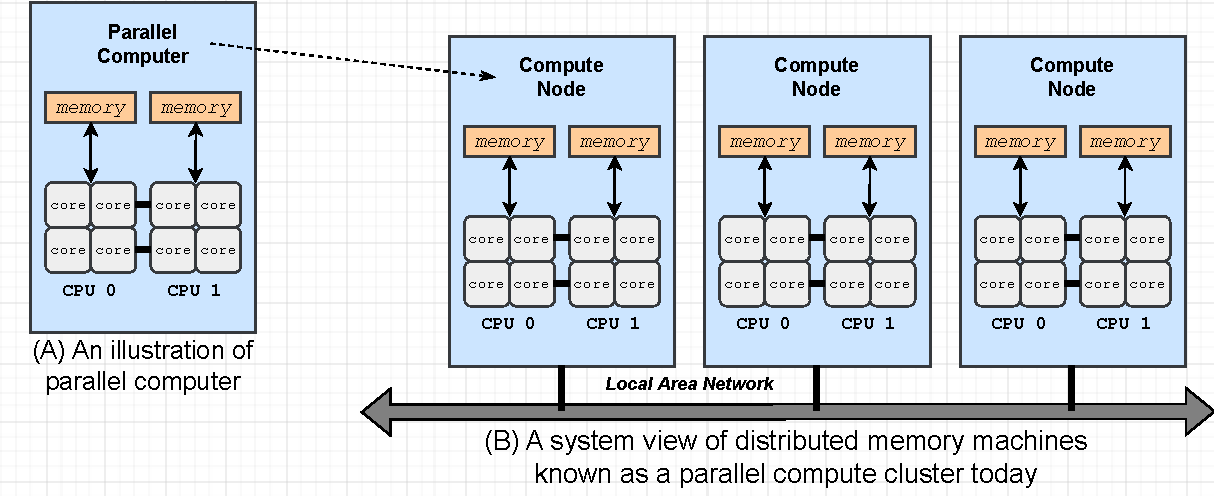
\includegraphics[scale=0.6]{./pictures/preliminaries/preli_parallel_and_distributed_memory_machines.pdf}
	\caption{An example of parallel computers and distributed memory systems know as a parallel compute cluster.}
	\label{fig:preli_parallel_computer_and_cluster}
\end{figure}

\noindent \textbf{Parallel computers:} refers to a computer or a machine with more than one processor (CPU). Sometimes, people imply a CPU as a CPU socket, the physical interface on a motherboard where a CPU is located. In modern computing architectures, a CPU contains multiple cores called single processing units, and each core can execute instructions independently. Each CPU can have its individual memory, where the total memory in a parallel computer is the sum of all individual memories. Figure \ref{fig:preli_parallel_computer_and_cluster} (A) reveals an example of a parallel computer with two CPUs, each with its own memory and containing four cores.\\

Memory access in parallel computers is a complex topic. We can also use the types of memory access to characterize the type of parallel computers. There are mainly two types, shared memory and distributed memory. Shared memory can be noted with all processors accessing the same memory, or a so-called shared address space. Distributed memory can be seen that each CPU has a memory and each refers to a variable on its own memory.\\

From the view of hardware manufactures, the memory architectures of parallel computers are known as
\begin{itemize}
	\item Uniform Memory Access (UMA): all memory locations are accessible to all processors. The access time can be assumed to be identical. A limitation of UMA is the maximum number of processors that can be difficult to expand.
	
	\item Non-Uniform Memory Access (NUMA): each process has a separate memory. This memory architecture can deal with the limit of UMA but leads to a situation where a processor or the cores of a processor access its own memory (local memory) fast and access the other processors' memory (remote memory) slower. Distributed memory implies that a processor cannot directly see another processor's memory. From the programmer's view, there can be a reference to physically and logically distributed memory, which means whether memory is distributed or just appears distributed \cite{victor2010introhpc}. NUMA can be seen as logically and physically distributed, although the distributed nature of NUMA is not apparent to the programmer. Today, most modern computers are made with multicore processors and NUMA architectures.
\end{itemize}

In general, the goal of using parallel computing is to get higher computation performance and access more memory. However, as scientific problems scale up, the complexity of solving them can take a long time to execute on a single computer. Therefore, the idea of parallel compute clusters was built and widely used.\\

\noindent \textbf{Parallel compute clusters:} refers to the architecture used in most supercomputers today. Parallel compute clusters are examples of distributed memory systems. A cluster consists of many computers; in particular, we imply many parallel computers, as explained above. The computers in a cluster are so-called compute nodes. Figure \ref{fig:preli_parallel_computer_and_cluster} (B) demonstrates a parallel compute cluster. All compute nodes can operate as a unified system. Each node connects to another via a local area network (the so-called interconnection network) \cite{baker1999cluster}. The exchange of data or messages between different processors across different nodes is physically distributed memory, where communication overhead might affect the performance of parallel applications. In this thesis, distributed memory indicates the view of memory access in parallel compute clusters. \\

\noindent \textbf{Terminologies}: summarize and emphasize several terminologies based on the explanation above. The following might repeat some notations as well as terms used throughout the thesis.

\begin{itemize}
	\item Cluster: denotes a parallel compute cluster, and is also called an HPC cluster, HPC system, or supercomputer.
	
	\item Node: indicates a compute node in a cluster. Inside a compute node, we have
	\begin{itemize}
		\item Processor or CPU: indicates central processing unit. In computer hardware, a CPU is placed in a CPU socket, which contains mechanical components providing mechanical and electrical connections between a microprocessor and a printed circuit board (PCB). Sometimes, a mentioned CPU socket can also be understood as referring to a CPU.
		\item Core: is single processing unit in a processor. There can be multiple cores inside a processor. Different cores in a node can belong to the same processor or different processors. At the operating system (OS) level, there are
		\begin{itemize}
			\item Process: is an instance of a program. When a process is created and executed, it is defined with its own resources, e.g., memory, file descriptors.
			\item Thread: is an entity within a process. A process can spawn multiple threads inside. While processes are isolated, threads share memory and address space.
		\end{itemize}

		Depending on context switching and mapping algorithm, processes or threads can be mapped dynamically to cores. For performance purposes, a process or thread is often pinned to a specific core in HPC, reducing context switching time. Furthermore, a technology introduced by manufacturer Intel is hyperthreading (Hyper-Threading Technology as HTT or HT) that a single core can run multiple threads. In this case, we call them logical cores in a physical core.
		
	\item Memory: this thesis refers to NUMA architecture in a node (NUMA domain). Each CPU has an individual memory, often called a NUMA node. However, we avoid using NUMA node to ensure no conflict with ``node'' in compute node. We consider the view of memory access in a single node as shared memory. Therefore, it is important to note that
		\begin{itemize}
			\item Shared memory: indicates memory access in a single node.
			\item Distributed memory: indicates memory access across nodes.
		\end{itemize}
	\end{itemize}
	
	\item Communication: implies data or information exchange among processes. These processes can be inside a node or across nodes. To evaluate communication speed, bandwidth is defined as the maximum transmission performance of a network. Generally, bandwidth ($B$) today is measured by megabits, megabytes, or gigabytes per second (Mbps, MBps, or GBps). In HPC networks, communication overhead refers to
	\begin{itemize}
		\item Latency ($\lambda$): the delay time between sending and receiving the header of a message. $\lambda$ can be measured in seconds or milliseconds.
		\item Transmission time or Delay time ($d$): the time for transmitting an entire message between two nodes. Delay ($d$) depends on the size of a message. In the case of no conflict, $d = \lambda + \frac{s}{B}$, where $s$ is the message size. 
	\end{itemize}

\end{itemize}

From the application perspective, users can implement parallel applications using different programming models. The next section introduces general and widespread parallel programming models in common use. Following that, we emphasize our focus on task-based parallel programming models and task-based parallel applications to deal with dynamic load balancing.


% Regarding MPI applications, we might use ranks as an alternative name for processes. Therefore, rank and process can be used interchangeably.
	
%	\item Task: there are different ways to define a task. People may call a task a discrete logical section of computational work. In another context, a task can be a program or a set of instructions executed in sequential or parallel by one or multiple threads/processes. In the thesis's context, we define a parallel program with many tasks.

%	\item Synchronization: denotes the coordination of parallel tasks in real-time. The downsize of synchronization implies waiting for at least one task. Therefore, it can cause a parallel application's wall clock execution time.
%
%	\item Computational Granularity: implies a quantitative or qualitative measure between computation and communication. There are two common terms: \textit{coarse} and \textit{fine}.
%	\begin{itemize}
%		\item Coarse: indicates many computational tasks between communication events.
%		\item Fine: means a small number of computational tasks between communication events.
%	\end{itemize}
%
%	\item Speedup: is a ratio of wallclock execution time between serial execution and parallel execution.
%
%	\item Parallel Overhead: is related to the required execution time, including influence factors such as task start-up time, synchronization, data movement, software overhead, and task termination time.
%
%	\item Scalability: is associated with the ability of a parallel system that can show a proportionate increase in speedup. Several factors, such as hardware, application algorithm, parallel overhead, and application characteristics, can contribute to scalability.

%\textbf{Architectures}: parallel computing systems are mainly designed upon memory models. Almost all machines today revolve around three architectures: shared memory, distributed memory, and hybrid distributed-shared memory.
%\begin{itemize}
%	\item Shared memory machines: is commonly designed with the ability of all processors to access memory like global address space. This architecture has been classified as Uniform Memory Access (UMA) and Non-Uniform Memory Access (NUMA, as mentioned). UMA is  Symmetric Multiprocessor (SMP) with identical processors and equal access time to memory. In contrast, NUMA has a physical link between two or more SMPs. One SMP can access the memory region of another SMP, and they will not have equal access time due to across links.
%	\item Distributed memory machines: often implies a communication overhead via network to link one processor's memory to another. We do not have global address space across all processors because each has its own local memory. Programmers have to define how and when tasks or data are communicated. Importantly, synchronization is essential, and it often belongs to the programmer's responsibility
%	\item Hybrid distributed-shared memory machines: ``hybrid'' refers to the memory model that works on both CPU and graphic processing unit (GPU)/accelerators. There are two main components: shared memory component and distributed memory component. The shared component indicates the connection between CPU and GPU, while the distributed component means the connection between multiple CPU/GPU machines. The current trends show that this computing architecture will be more and more popular in future computing technologies.
%\end{itemize}

%	%---------------------------------
%	\item Distributed memory systems
%	%---------------------------------
%	\begin{itemize}
%		\item Fixed: the number of connections between nodes is fixed. When more processors or nodes are added, they have to share, e.g., Ethernet interconnection.
%		\item Linear: the number of connnections grows linearly when the number of nodes is increased, e.g., mesh-based interconnection.
%		\item Scalable: the number of connections grows as $P\log P$ or even greater, e.g., hypercube interconnection.
%	\end{itemize}
%\end{itemize}

%\input{content/Related-Work}

%\vfill
%\section*{Chapter Summary}
%Chapter~\ref{ch:Motivation} provides the motivation, scopes the problem and derives a requirements' analysis for
%a reference model for \pne management systems for \glspl*{HPC system}.
%Additionally, the related work is presented.
%This presents the problem domain analysis according to the methodical approach of this work (see Sec.~\ref{sec:Intro-Method}).
%
%\begin{figure}[H]%[ht]
%    \centering
%    \resizebox{.98\textwidth}{!}{%
%        \input{pictures/Thesis-Method-Gray/Thesis-Method-Gray2.tikz}
%        }
%        \caption[Method Completion After Chapter 2.]{%
%            Method completion after Chapter 2.}
%            \label{fig:Method-Completion2}
%\end{figure}


% 2.1 Parallel Programming Models
\section{Task-based Parallel Programming Models}
\label{sec:taskbased_prog_models}
\index{FromWS2ReactLB!Parallel Programming Models}
% ---------------------------------
% Example for using \si command
% ---------------------------------
% In the advance from \si{peta\gls*{FLOPS}} to \si{exa\gls*{FLOPS}} performance the issues of \pne present a major hurdle. The associated challenges are identified and tackled by different entities in various ways.

A programming model forms an abstraction layer that connects user applications and parallel computer architectures, leveraging a programming-support library/runtime. Before the advent of task-based parallel programming models, shared and distributed memory models have been used mainly. However, there is no clear boundary of these models. The model design relies on the development of computing and memory architectures, such as multicore, manycore, NUMA architectures. The following introduces conventional models, then details the principle of task-based parallel models.\\

\begin{figure}[t]
  \centering
  \includegraphics[scale=0.485]{./pictures/preliminaries/preli_conventional_parallel_prog_models.pdf}
	\caption{An overview of shared memory and distributed memory programming models along with their hybrid model.}
	\label{fig:preli_conventional_parallel_prog_models}
\end{figure}

\noindent \textbf{Shared Memory Programming Model}: enables processes or threads to share a common address space. In this model, processes or threads can communicate and synchronize by reading/writing directly from/to shared memory locations. The model allows efficient data sharing. Figure \ref{fig:preli_conventional_parallel_prog_models} (A) illustrates a parallel program using shared memory programming with threads. Here, Thread 0, 1, 2 execute the instructions simultaneously, and the data such as array A and array B are shared. Shared memory programming can be characterized by:
\begin{itemize}
	\item Advantage: simple and straightforward to write programs in parallel. Communication between processes/threads is faster and more efficient than other models requiring inter-process communication.
	\item Disadvantage: difficult to manage data locality. There are challenges in dealing with complex synchronization, race conditions. Incorrect management of shared memory locations can lead to bugs. Furthermore, the scalability might be limited in the scope of a single machine.
	\item Implementation: the most common library is POSIX threads (so-called Pthreads) \cite{butenhof1997programming}. Besides that, OpenMP \cite{dagum1998openmp} is an industry-standard library to support shared memory programming, widely used in various operating systems and compilers. 
\end{itemize}

%\item Threads model: denotes parallel programs using threads. A heavy process can spawn multiple ``lightweight'' threads with concurrent execution paths. Besides POSIX standard, there is another popular API named OpenMP , an industry standard that is easy to use with directive-based declaration.
%This might be considered as the simplest parallel programming model, but sharing can raise contention problems such as race conditions, deadlocks. Various mechanisms called locks/semaphores are proposed. The model has some characteristics as follows.
%Besides, as mentioned, several implementations working on distributed memory machines can also work with shared memory, for example, SHMEM \cite{chapman2010introducing}. Therefore, people often refer to shared memory with or without threads.

\noindent \textbf{Distributed Memory Programming Model}: does not have a shared address space. Distributed memory in this thesis points to physically distributed memory systems where compute nodes connect to each other via a network. Note that memory architectures can also be called distributed in a single machine with NUMA architecture. However, it just appears as distributed memory from the programming view. We demonstrate a distributed memory programming example in Figure \ref{fig:preli_conventional_parallel_prog_models} (B), assuming we have two compute nodes, each creates a process to execute parallel application. The only way to exchange information across these nodes is message passing. For example, Process 2 sends a message to Process 1 and vice versa. Distributed programming models can be characterized by:
\begin{itemize}
	\item Advantage: data and information are exchanged explicitly by sending and receiving messages. Programmers can coordinate nodes to execute tasks and share data on large problems. The scalability of this model is well-suited for HPC and large-scale parallel applications.
	\item Disadvantage: communication overhead is challenging in data decomposition and combination. The problem in a distributed memory model is divided into smaller parts, which are distributed over nodes. After execution, their results and required data need to be combined, which may take time and overhead. Load balancing is also a challenge when task distribution is irrelevant to the system performance model.
	\item Implementation: the most popular library is based on the Message Passing Interface (MPI) standard \cite{gropp1996mpich}. MPI supports API and subroutines that users can define data exchange communication explicitly or implicitly. Besides, several libraries that support message passing at higher levels can also be characterized as distributed memory programming models known as Partitioned Global Address Space (PGAS) \cite{dewael2015pgasl}. PGAS provides an abstraction layer for programmers. We may not need to define the communication of data exchange explicitly. In this thesis, we classify the programming models like PGAS as data-parallel programming models.
\end{itemize}

\noindent \textbf{Data Parallel Programming Model}: refers to Partitioned Global Address Space (PGAS) \cite{dewael2015pgasl}. The idea is to achieve a higher level of abstraction from a programmers perspective. Even on shared or distributed memory, it treats address space globally. For example, the global data structure can be split up logically across tasks in distributed memory systems. Data parallel programming can be characterized by:
\begin{itemize}
	\item Advantage: user-friendly from the programming point of view. The model shows considerable benefits on regular data structures like arrays or matrices.
	\item Disadvantage: in some use cases with complicated data structures, this model cannot ensure performance as well as portability, such as data locality references, the distribution of sparse and irregular data objects. These are important issues for evaluating the efficiency of data-parallel programming models.
	\item Implementation: several implementations such as Coarray Fortran \cite{mellor2009new}, UPC \cite{zheng2014upc}, X10 \cite{chrles2005x10}, Chapel \cite{chamberlain2007chapel}.
\end{itemize}

\noindent \textbf{Hybrid Programming Model}: refers to combining more than one programming model. We have mentioned the hybrid model of shared memory and distributed memory programming, such as MPI+X or MPI+OpenMP \cite{rabenseifner2009hybrid} in Chapter \ref{ch:Introduction}. Shared memory programming models such as OpenMP allow users to specify shared memory locations and threads, but the scalability is limited in a single node. Distributed memory programming models such as MPI allow users to specify communication patterns and processes across nodes. A MPI process is denoted as MPI rank. In MPI-based applications, message passing can occur inside a node when we fully create the number of MPI ranks corresponding to the number of cores. Therefore, the hybrid model exploits benefits from both shared memory and distributed memory programming, such as reducing unnecessary MPI communication inside a node, overlapping communication and computation. Technically, a multicore processor within a node only needs to create one MPI process, where this process can spawn multiple threads. One or a few threads take care of MPI communication while the others execute computation tasks. With the trend of heterogenous computing architectures today, this model is the most relevant. Heterogeneous computing architectures are then implemented as CPUs accelerated by graphics processing unit (GPU) architectures \cite{zhang2011gpumodel}, which are widely used in today's HPC clusters and supercomputers \cite{top500list}. Generally, hybrid models can be characterized by:
\begin{itemize}
	\item Advantage: enables overlapping communication and computation and dealing with data locality. This can be applied similarly for CPU-GPU applications in distributed memory systems, where one or a few threads control communication across nodes, the other threads control computation tasks run on CPU or offloaded to GPU.
	\item Disadvantage: traditional parallel applications need to be changed following the hybrid model. This might lead to conflicts if support libraries or frameworks cannot control the mix of multiple processes along with multiple threads. Furthermore, the hybrid programming model such as MPI+OpenMP might also require users' effort to change conventional applications with pure MPI or pure OpenMP.
	\item Implementation: MPI+OpenMP as an example. Besides OpenMP, MPI can also combine with Pthreads for supporting multithreading inside a process.
\end{itemize}

Figure \ref{fig:preli_conventional_parallel_prog_models} (C) shows an example of a hybrid MPI+OpenMP programming model. The illustrated application is executing on two compute nodes ($Node\ 1$ and $Node\ 2$). Each node deploys an MPI process, $Process\ 1$ belonging to $Node\ 1$ and $Process\ 2$ belonging to $Node\ 2$. Each process spawns three OpenMP threads, where $Thread\ 0$ and $Thread\ 1$ execute the main computation parts, while $Thread\ 2$ is dedicated to performing communication.\\

\begin{figure}[t]
  \centering
  \includegraphics[scale=0.65]{./pictures/preliminaries/preli_task-based_prog_model.pdf}
	\caption{An overview of task-based parallel programming model.}
	\label{fig:preli_taskbased_programming_model}
\end{figure}

\noindent \textbf{Task-based Parallel Programming Model}: is a higher abstraction model based on the hybrid programming model. With the previous programming models in general as well as the hybrid model in specific, it is difficult to manage concurrency issues effectively. Furthermore, today's perspective of low-level programming, such as better performance by tightly controlling hardware, has been changed because users have to make an effort to optimize code among computation, communication, and synchronization. For example, synchronization barriers are often declared in shared and distributed memory programming models and require the user's responsibility. This can lead to performance issues, e.g., causing much idle or waiting time, if we do not control the synchronization tightly.\\

Task-based parallel programming models focus on the criteria of user-friendly coding, portability, and well-expressing parallelism.
The idea of task-based models is to separate the part of tasks, that need to be computed, from the part of computing resources in parallel execution. Users can reduce the burden of controlling how tasks are executed, synchronized, or parallelized. Instead, we just need to define what tasks are, their relationship, and whether they are dependent or independent. Dependent tasks can be represented as a graph of tasks, which is a so-called task graph. An interesting case study formulated as a task graph is game engine \cite{regragui2022schedgameengine}, which is studied to explore task scheduling by Regragui et al.\\

Figure \ref{fig:preli_taskbased_programming_model} illustrates an example of task-based parallel programming. From left to right, the application is assumed to be transformed into a set of tasks. Task transformation depends on how we define a task. A task often points to a compute code entry and its data. The way of transforming tasks or porting normal applications into task-based applications is called tasking. In Figure \ref{fig:preli_taskbased_programming_model}, we assume two cases of task transformation: independent and dependent. The dependent tasks can be addressed as a graph. The next step is queuing and scheduling tasks. Assume we have two compute nodes, $Node\ 1$ and $Node\ 2$. Tasks assigned to $Node\ 1$ are queued and scheduled for execution on $Node\ 1$. Similarly, tasks assigned to $Node\ 2$ are queued and scheduled for execution on $Node\ 2$. Following this, executing tasks on each node is controlled by the task-based programming model, which is usually implemented as a library or framework. During execution, the task-based programming model controls mapping tasks to threads for computation; thus, a task-based model is also called a task-based runtime. After computation, the application's working flow is returned to users.\\

In Figure \ref{fig:preli_taskbased_programming_model}, the view of computing resources on $Node\ 1$ and $Node\ 2$ is similar to the hybrid model, where each node contains a process, a process spawns a pool of threads for task execution. However, users only need to define tasks and are relaxed in managing parallelization, communication, concurrency, or synchronization. We characterize task-based models as follows.
\begin{itemize}
	\item Advantage: user-friendly to develop parallel applications. We can simplify parallel applications with tasks and task relationships. It can be easier to control synchronization and concurrence.
	\item Disadvantage: porting applications from conventional to task-based models might lead to performance issues. Besides, defining tasks in some specific applications is sometimes difficult.
	\item Implementation: there are more and more libraries or frameworks developed to support task-based parallel programming, such as StarPU \cite{augonnet2011starpu}, OmpSS \cite{duran2011ompss}, HPX \cite{kaiser2014hpx}, Taskflow C++ \cite{huang2020cpp}, etc. They are developed in different languages like C++, Python.
\end{itemize}

The next section will show how task-based parallel runtimes are categorized and how task-based parallel applications are characterized in terms of performance issues.

%The idea of task-based programming is not new, where tasks are represented independently or dependently as a graph of tasks (the so-called task graph). Task graphs have been used to model and optimize parallel execution since the early history of computers \cite{codd1960multiprogram}. However, people applied this to the whole jobs instead of defining small tasks in a single application. 

%For task-based programming models, users can reduce effort by expressing tasks and their dependencies without specifying synchronization and concurrence.
%Today, many libraries or runtimes already support task-based models, such as OpenMP tasking \cite{ayguade2008design}, HPX \cite{kaiser2014hpx}, Charm++ \cite{acun2014parallel}.

% 2.2 Task-based Parallel Runtimes and Applications
\section{Task-based Parallel Runtimes and Applications}
\label{sec:taskbased_runtimes_apps}
\index{FromWS2ReactLB!Task-based Parallel Runtimes Apps}
Tasks can appear in different contexts. For example, we often use tasks to indicate a code region in shared and distributed memory programming models. However, this definition is loose and not clear to determine where is the task space and which is the task data or task input/output.\\

In task-based parallel programming, tasks are defined more consistently. We define a task by a code entry and its data. The data indicate input, output, or data region that a task can manipulate. When the input/output of a task is associated with other tasks, these tasks are dependent. Porting a normal application into a task-based one can help simplify the parallel execution such a well-expressed parallelism.\\

In terms of execution, a specific implementation of task-based programming models is considered as a library or a framework. This library attempts to separate parallel programs into a pool of tasks and a pool of computing resource units. The pool of computing resource units indicates threads within a process. These two pools imply two levels: application level and system level. From the application level, we can see task-based applications as a black box. From the system level, we can see task-based programming models as runtimes. The runtimes manage tasks and handle performance portability \cite{aumage2021taskportability}. Performance portability means:
\begin{itemize}
	\item Users can simplify parallel applications as tasks alongside their data.
	\item Users can quickly port parallel applications to new and different platforms.
	\item Users can be relaxed in terms of task scheduling, load balancing, and overlapping communication-computation at the side of task-based runtimes.
\end{itemize}

% Note: definition between framework, library, api
% 	+ library: a collection of code (e.g., functions, objects) to perform common tasks. It tends to be stable and bug free. Using appropriate libs can reduce the amount of code that needs for writting the program.
%		+ API (Application Programming Interface): provides some functionality which allows an application to access the available functionality. It exists at many levels including system, library, framework, program.
% 	+ Framework: is a collection of APIs designed to make building of application simpler.
%
%		-------------------
%		- Framework 			-
%		-------------------
%		- Library   			-
%		-------------------
%		- API       			-
%		-------------------

Based on the survey of Thoman et al. \cite{thoman2018taxonomy}, we summarize the main characteristics for classifying task-based parallel programming runtimes. These characteristics refer to application programming interfaces (API) in a given task-based runtime, which can be developed like a library, a language extension, or a language. The classification has four aspects: Architecture, Task System, Task Management, and Engineering. Table \ref{tab:taskbased-apis} summarizes this classification associated with various task-based runtimes and libraries today.

\begin{itemize}
	\item Architecture: highlights the target systems or computer architectures. In detail, the related factors of architecture are further divided into three components.
		\begin{itemize}
			\item Communication model: shared memory, message passing, and an abstraction model called global address space, which is created as a shared memory model for distributed memory systems. These terms are denoted by $smem$, $msg$, $gas$, respecively in Table \ref{tab:taskbased-apis}.
			\item Distributed memory system: the compatibility with distributed memory is explicit, implicit, or no support. The terms of ``implicit'', ``explicit'', ``no support'' are denoted by $i$, $e$, \xmark, respectively.
			\item Heterogeneity: indicates whether tasks can be ported to accelerators or not. The classification is also denoted by explicit, implicit, or no support with $i$, $e$, and \xmark, respectively.
		\end{itemize}
		
	\item Task System: shows how tasks are built and simplified with or without dependencies. The main factors are structure and task partitioning. Furthermore, we can also classify them by result handling and task cancellation.
		\begin{itemize}
			\item Graph structure: the possibilities of representing task dependency include tree ($tree$), acyclic graph ($dag$), arbitrary graph ($graph$), or no dependency.
			\item Task partitioning: indicates whether a task is atomic ($atom$ or \cmark) or can be divisible ($div$ or \xmark).
		\end{itemize}
	
	\item Task Management: is related to task assignment and resource management. Moreover, this characteristic focuses on how tasks are supported for resilience as well as debugging.
		\begin{itemize}
			\item Worker management: indicates whether the worker threads/processes (which execute tasks) are maintained ``explicit'' by users or ``implicit'' (automatically) by the environment.
			\item Work mapping: describes the strategy that tasks are assigned to computing resource units. The possibilities include ``explicit'' mapping or ``implicit'' mapping.
		\end{itemize}
		
	\item Engineering: shows how a task-based programming interface is used or implemented, such as a library ($lib.$), a language extension ($ext.$), or a language ($lang.$).
\end{itemize}

\begin{table}[t]
\centering
\scalebox{0.9}{
\begin{tabular}{|l|lll|ll|ll|l|}
\hline
\multirow{2}{*}{\textbf{APIs}} & \multicolumn{3}{c|}{\textbf{Architecture}} & \multicolumn{2}{c|}{\textbf{Task System}} & \multicolumn{2}{c|}{\textbf{Task Management}} & \multicolumn{1}{c|}{\multirow{2}{*}{\textbf{Engineering}}} \\ \cline{2-8}
		& \multicolumn{1}{l|}{\rotatebox{270}{Communication model }} & \multicolumn{1}{l|}{\rotatebox{270}{Distributed memory}} & \rotatebox{270}{Heterogeneity} & \multicolumn{1}{l|}{\rotatebox{270}{Graph structure}} & \rotatebox{270}{Task partitioning} & \multicolumn{1}{l|}{\rotatebox{270}{Worker management}} & \rotatebox{270}{Work mapping} & \multicolumn{1}{c|}{}                             \\ \hline
	C++ STL \cite{kormanyos2015} & \multicolumn{1}{l|}{smem} & \multicolumn{1}{l|}{\xmark} & \xmark & \multicolumn{1}{l|}{dag} & \xmark & \multicolumn{1}{l|}{\textbf{i}} & \textbf{i/e} & lib. \\ \hline
	TBB \cite{willhalm2008putting} & \multicolumn{1}{l|}{smem} & \multicolumn{1}{l|}{\xmark} & \xmark & \multicolumn{1}{l|}{tree} & \xmark & \multicolumn{1}{l|}{\textbf{i}} & \textbf{i} & lib. \\ \hline
	HPX \cite{kaiser2014hpx} & \multicolumn{1}{l|}{gas} & \multicolumn{1}{l|}{i} & \textbf{e} & \multicolumn{1}{l|}{dag} & \cmark & \multicolumn{1}{l|}{\textbf{i/e}} & \textbf{i/e} & lib. \\ \hline
	Legion \cite{bauer2014legion} & \multicolumn{1}{l|}{gas} & \multicolumn{1}{l|}{i} & \textbf{e} & \multicolumn{1}{l|}{tree} & \cmark & \multicolumn{1}{l|}{\textbf{i}} & \textbf{i/e} & lib. \\ \hline
	PaRSEC \cite{hoque2017dynamic} & \multicolumn{1}{l|}{msg} & \multicolumn{1}{l|}{e} & \textbf{e} & \multicolumn{1}{l|}{dag} & \xmark & \multicolumn{1}{l|}{\textbf{i}} & \textbf{i/e} & lib. \\ \hline
	Chameleon \cite{Klinkenberg2020ChameleonReactLB} & \multicolumn{1}{l|}{msg} & \multicolumn{1}{l|}{e} & \xmark & \multicolumn{1}{l|}{dag} & \cmark & \multicolumn{1}{l|}{\textbf{e}} & \textbf{i/e} & lib. \\ \hline
	Taskflow \cite{huang2020cpp} & \multicolumn{1}{l|}{smem} & \multicolumn{1}{l|}{\xmark} & \textbf{e} & \multicolumn{1}{l|}{dag} & \cmark & \multicolumn{1}{l|}{\textbf{i/e}} & \textbf{i/e} & lib. \\ \hline
	OpenMP \cite{ayguade2008design} & \multicolumn{1}{l|}{smem} & \multicolumn{1}{l|}{\xmark} & \textbf{i} & \multicolumn{1}{l|}{dag} & \xmark & \multicolumn{1}{l|}{\textbf{e}} & \textbf{i} & ext. \\ \hline
	Charm++ \cite{acun2014parallel} & \multicolumn{1}{l|}{gas} & \multicolumn{1}{l|}{\textbf{i}} & \textbf{e} & \multicolumn{1}{l|}{dag} & \cmark & \multicolumn{1}{l|}{\textbf{i}} & \textbf{i/e} & ext. \\ \hline 
	OmpSs \cite{duran2011ompss} & \multicolumn{1}{l|}{smem} & \multicolumn{1}{l|}{\xmark} & \textbf{i} & \multicolumn{1}{l|}{dag} & \xmark & \multicolumn{1}{l|}{\textbf{i}} & \textbf{i} & ext. \\ \hline
	StarPU \cite{augonnet2011starpu} & \multicolumn{1}{l|}{smem} & \multicolumn{1}{l|}{\textbf{e}} & \textbf{e} & \multicolumn{1}{l|}{dag} & \cmark & \multicolumn{1}{l|}{\textbf{i}} & \textbf{i/e} & ext. \\ \hline
	Cilk Plus \cite{robison2012cilk} & \multicolumn{1}{l|}{smem} & \multicolumn{1}{l|}{\xmark} & \xmark & \multicolumn{1}{l|}{tree} & \xmark & \multicolumn{1}{l|}{\textbf{i}} & \textbf{i} & lang. \\ \hline
	X10 \cite{chrles2005x10} & \multicolumn{1}{l|}{gas} & \multicolumn{1}{l|}{\textbf{i}} & \textbf{i} & \multicolumn{1}{l|}{dag} & \cmark & \multicolumn{1}{l|}{\textbf{i}} & \textbf{i/e} & lang. \\ \hline
\end{tabular}}
\caption{An overview of the programming interface characteristics in various task-based parallel programming runtimes.}
\label{tab:taskbased-apis}
\end{table}

% Some relevant issues researched in task-based models might be listed as follows.
%\begin{itemize}
%	\item Continue to improve data locality decisions with more expressive abstractions of tasking.
%	\item Attempt to extend low-level resource management in HPC systems.
%	\item Relax application porting in more realistic use cases.
%	\item Support interoperability and proactive directions in scheduling and balancing tasks/loads.
%\end{itemize}

\clearpage

% ------------------------------------
% About task-based parallel applications
% ------------------------------------

\begin{figure}[t]
	\centering
	\includegraphics[scale=0.725]{./pictures/preliminaries/preli_task-based_app_usecases.pdf}
	\caption{Three examples illustrated as the three use cases of task-based parallel applications.}
	\label{fig:preli_taskbased_apps}
\end{figure}

\noindent There are three common use cases for porting an application to a task-based parallel application. They are known as recursion, complex synchronization, overlapping computation and communication for numerical simulations. These three use cases are illustrated in Figure \ref{fig:preli_taskbased_apps}, including (A) Fibonacci, (B) Cholesky factorization, and (C) Adaptive Mesh Refinement.\\

The task-based version of Fibonacci defines tasks by its compute function (named \texttt{fib(n)}). The input data of tasks is an integer number. All tasks are generated recursively, tasks nested in another task. Using task-based parallel programming, we can facilitate the parallelism in Fibonacci with cut-off strategies as shown in Figure \ref{fig:preli_taskbased_apps} (A).\\

For Cholesky factorization, the difficulty is complex synchronization patterns. Porting Cholesky to a task-based parallel version can improve composability and clarify synchronization patterns. As shown in Figure \ref{fig:preli_taskbased_apps} (B), the program behavior is broken into separate tasks, such as computing factorization (\texttt{fac}), triangular solver (\texttt{tri}), matrix multiplication (\texttt{mat}), update (\texttt{upd}) as well as synchronization.\\

The rest is an example of Adaptive Mesh Refinement shown in Figure \ref{fig:preli_taskbased_apps} (C). It is known as a typical approach of numerical simulations in HPC. Here, tasks are defined by the function of traversing grid/mesh cells (denoted by \texttt{trav}). These tasks are independent, and their input data depends on the constraint parameters of simulation contexts, e.g., earthquake, tsunami. Executing Adaptive Mesh Refinement comprises multiple computation phases interwoven with synchronization phases, also called iterative execution. When running in distributed memory systems, each node executes an assigned part of the given grid. Therefore, there might be communication for exchanging grid information to compute the tasks. Using task-based programming, communication and computation can easily overlap. Especially the isolation between a pool of tasks and a pool of resources helps facilitate a dedicated communication thread by exchanging information during computation. Furthermore, Prat et al. \cite{prat2018taskbasedmdsim} also show the efficiency of task-based parallelism with another example, molecular dynamics (MD) simulations. Their MD implementation is $4.7\times$ faster than the state-of-the-art implementations (LAMMPS \cite{lammps2008mdsim}).\\

\noindent Task-based parallel runtimes help to simplify parallel programming. It is easier to manage tasks and control resources by separate pools. This offers an advantage for solving dynamic load balancing in distributed memory systems. The following section details how load balancing is formulated in task-based parallel applications and related work. 


% 2.3 Load Balancing in Parallel Programs
\section{Related Work}
\label{sec:relatedwork}
\index{FromWS2ReactLB!Related Works}

\subsection{Dynamic Load Balancing} \label{subsec:dlb}

This work revolves around load balancing problems in distributed memory systems. Our target objects are task-based parallel applications, where the main use case is shown in Figure \ref{fig:preli_taskbased_apps} as iterative execution of HPC numerical simulations.\\

In general, load balancing is to treat each process an equal share of the total load \cite{cybenko1989dynamic}. Almost all problem contexts and solutions are broadly categorized into ``static'' and ``dynamic''.\\

``Static'' relies on a $priori$ knowledge of load, implying that the static methods are performed before execution. People assume the given cost models are stable at runtime, which is feasible to generate optimal balancing algorithms. There are three simplified branches of static balancing methods:
\begin{itemize}
	\item Static optimal task distribution
	\item Static optimal thread/process assignment
	\item Approximate or heuristic task scheduling
\end{itemize}

Static load balancing works optimally in ideal systems with a stable performance model. All processors execute tasks at the same speed. We can manipulate tasks, threads, or processes to balance the load. In principle, finding an optimal algorithm of load balancing for more than two processes is studied and addressed as an NP-hard problem \cite{bokhari1981mapping}, \cite{bokhari1988partitioning}. Under certain assumptions about the application behavior or system characteristic, there are several studies about the optimal algorithms for task distribution and thread/process assignment, such as \cite{bokhari1987assignment}, \cite{nicol1996static}. Another direction is heuristic algorithms, which are also common because of their simplicity in implementation \cite{benmohammed1991evallb} \cite{bowen1992assignment}. The advantage of static load balancing is minimizing runtime overhead and is suitable when the execution time of tasks can be estimated before execution. \\

\begin{figure}[t]
	\centering
	\includegraphics[scale=0.7]{./pictures/preliminaries/preli_balance_vs_imbalance_by_perfslow.pdf}
	\caption{Balance vs imbalance in the case of executing tasks on 8 processes.}
	\label{fig:preli_balance_vs_imbalance_by_perfslow}
\end{figure}

% This work distinguishes the optimal distribution algorithms that often focus on a given number of tasks distributed on many processes.
% With the advantage of tasking, tasks and computing resources are isolated, which can be flexible to control mapping, scheduling, and migrating tasks around. The main perspective of this work is based on task-based programming models to show our proactive approach to balancing the load of parallel applications in distributed memory. From a top-down overview, this section summarizes the balancing problems in HPC associated with their constraints. Importantly, we attempt to introduce their related solutions as well as the state-of-the-art directions in this topic. Following that, we lead to the motivation why the thesis focuses on a proactive balancing approach.\\

``Dynamic'' or dynamic load balancing (DLB) is more suitable when load and performance models are unknown or variable at runtime. The cost models might also be varied during execution. For example, unexpected performance slowdown affects the load values of tasks. \\

As introduced in Section \ref{sec:intro_prob_form_motiv}, we summarize again our imbalance context here. Assume that a parallel application is simplified as tasks by a given distribution of $T$ tasks on $P$ processes. Each process is assigned a subset of tasks $T_{i}$, where $i$ indicates the process index, $i \in \{0, ..., P-1\}$. Each task has a load value, $w_{j}$ where $j$ indicates the task index, $j \in T_{i}$. The total load value of a process is determined by the sum of load values associated with the tasks assigned to that process, i.e., $L_{i} = \sum_{j \in T_{i}} w_{j}$. Compared to the balanced case, we highlight the cause of the imbalance case in Figure \ref{fig:preli_balance_vs_imbalance_by_perfslow}, where (A) shows balance with a stable performance model, while (B) shows imbalance caused by performance slowdown in processes $P_{0}$, $P_{1}$, $P_{2}$, $P_{5}$. Each figure is a double-axis chart, in which the left x-axis reveals the execution flow from left to right; the green boxes illustrate tasks. The length of the boxes determines the length of task execution time. The right x-axis demonstrates the execution speed of each process, where the length of horizontal bars determines a low or high speed. Figure \ref{fig:preli_balance_vs_imbalance_by_perfslow} (B) emphasizes that performance might fluctuate during execution, and task migration is the only way to balance the load. Tasks should be migrated between a fast process and a slow process.\\

Regarding the evaluation metric, an imbalance is measured by a ratio calculated by maximum and average load values. In Section \ref{sec:intro_prob_form_motiv}, this ratio is named $R_{imb}$. We can use the total load values like $L_{i}$ to calculate $R_{imb}$, such as $L_{0}$, $L_{1}$, $L_{7}$ shown in Figure \ref{fig:preli_balance_vs_imbalance_by_perfslow} (B). Here, the maximum $L$ is $L_{5}$ (or $L_{2}$), and the average $L$ is named $L_{avg} = \frac{\sum_{i=0}^7 L_{i}}{8}$, where $P=8$ and $R_{imb} = \frac{L_{max}}{L_{avg}} - 1 = \frac{L_{2}}{L_{avg}} - 1$. If each process has multiple threads to execute tasks, $R_{imb}$ can also be calculated by the wallclock execution time per process, for example, $W_{avg} = \frac{\sum_{i=0}^7 W_{i}}{8}$.
\begin{itemize}
	\item If $R_{imb} \approx 0$, there is no imbalance.
	\item If $R_{imb} > 0$, there exists imbalance between the involved processes.
\end{itemize}

Corresponding to the imbalance, two groups of related parameters can directly or indirectly affect load balancing performance. Due to the isolation of computing resources between nodes in distributed memory systems, the only way to balance the load is moving tasks across processes or even across nodes. In the group of indirect parameters, we imply the parameters that affect imbalance level. In the group of direct parameters, we show the parameters that affect the performance of load balancing.\\

\begin{figure}[t]
	\centering
	\includegraphics[scale=0.9]{./pictures/preliminaries/preli_vectorspace_influparams.pdf}
	\caption{Direct and indirect parameters impact the performance of dynamic load balancing.}
	\label{fig:preli_params_vector_space}
\end{figure}

The green arrows of Figure \ref{fig:preli_params_vector_space} show the group of indirect parameters.
\begin{itemize}
	\item \textbf{Num. Processes} ($P$): the number of involved processes. This value might affect process selection algorithms for task migration and number of migrated tasks.
	\item \textbf{Execution Speed} ($S_{P}$): the execution speed of a process. The difference in execution speeds causes imbalance. The number of slow and fast processes affects imbalance level ($R_{imb}$). Notably, $R_{imb}$ can indirectly affect the number of migrated tasks.
	\item \textbf{Task Structure}: task system, where tasks can be dependent or independent, uniform or nonuniform load (determined by the $w$ values of tasks).
\end{itemize}

The blue arrows of Figure \ref{fig:preli_params_vector_space} show the group of direct parameters.
\begin{itemize}
	\item \textbf{Imbalance Ratio} ($R_{imb}$): imbalance level. It might challenge the applied balancing approaches because $R_{imb}$ might be high or low. For example, when $R_{imb}$ is very high, the number of migrated tasks can be large.
	\item \textbf{Num. Migrated Tasks} ($K$): the total number of migrated tasks. The number of migrated tasks at once (or per operation at a time) determines $K$. Therefore, getting an optimal value of $K$ can be seen as a necessary condition, and getting a reasonable number of migrated tasks at once to an adequate process can be seen as a sufficient condition.
	\item \textbf{Task Size}: the data size of a task. This size affects delay time when we migrate tasks. Importantly, the number of migrated tasks is also affected by data size.
	\item \textbf{Communication Overhead} (\texttt{Comm.Overhead}): indicates latency ($\lambda$) and delay time ($d$) in migrating tasks. The value of $d$ relies on the bandwidth ($B$) of a network and message size ($s$) \cite{peterson2021computer}. Communication overhead (\texttt{Comm.Overhead}) is considered as a constraint of performing load balancing in distributed memory systems, which can delay information exchange and task migration. The total load per process is changed when tasks are migrated from one process to another. Hence, the load balancing performance is changed when \texttt{Comm.Overhead} affects task migration. In detail, the definition and calculation of $\lambda$ and $d$ are explained in Section \ref{sec:preliminaries}.
%	\begin{itemize}
%		\item Latency ($\lambda$): the time of communication (between sending and receiving the header of a message).
%		\item Transmission time (delay $d$): the time for transmitting an entire message between two nodes. $d$ depends on the size ($s$) of a message and bandwidth ($B$). $B$ is measured as megabits or megabytes per second. If no conflicts exist, the delay is computed by $d(s) = \lambda + s/B$.
%	\end{itemize}
	\item \textbf{Victim Selection Algorithms}: indicates how we can choose an adequate process for migrating tasks, for example, in the case we have multiple victims. The selection algorithms directly affect how many tasks are migrated and which processes are good candidates.
\end{itemize}

% Additionally, throughput is also a common metric used to evaluate the performance of networks. Throughput is the ratio between message size and delay, in which the maximum throughput, in theory, is considered as the bandwidth.\\

As mentioned in Chapter \ref{ch:Introduction}, the most closely related approach is called ``work stealing'' \cite{Blumofe1999OriginWS}, which is common in shared memory systems. Also, we look upon shared memory systems as the group of load balancing without taking \texttt{Comm.Overhead} into account. The idea is to steal tasks from a busy process when the current process is idle. Many researchers have proposed methods for optimizing work stealing in terms of:

\begin{itemize}
	\item Algorithms: optimize the general strategies for stealing tasks. The algorithms are divided into \textit{nearest neighbor} (iterative) and \textit{global} (direct). The group of \textit{nearest neighbor} relies on successive approximations to a global optimal task distribution, and each balancing operation intends to task migration. These various methods are then categorized into \textit{deterministic} and \textit{stochastic}. On the one hand, \textit{deterministic} methods proceed according to the rules of predefined distribution. On the other hand, \textit{stochastic} methods distribute the tasks based on randomization.
	\begin{itemize}
		\item \textit{Deterministic} methods: diffusion \cite{halstead1980munet} \cite{sullivan1977large}, dimension exchange \cite{ranka1988programming}, and the gradient model \cite{lin1987gradient}. 
		\item \textit{Stochastic} methods: randomized allocation and physical optimization. Randomized allocation is the simplest method in that the victims of stealing tasks are randomly selected \cite{adler1998parallel}. Physical optimization is based on the analogies of parallel computers. These physical methods map a load balancing problem to a physical system and solve the problem using theoretical or experimental analysis by simulation \cite{rudolph1991simple}.
	\end{itemize}
	
	\item Task Selection: refers to algorithms that focus on selecting appropriate tasks to optimize work stealing. This branch of research is often proposed when we are concerned with topology-aware for dynamic load balancing. For instance, Vikranth et al. \cite{vikranth2013topoawarews} introduce a task stealing strategy that dynamically analyzes the topology of the underlying hardware connections for on-chip NUMA multicore processors. Their experiments have shown an average of 1.24$\times$ better performance on NAS\footnote{A small set of programs designed to help evaluate the performance of parallel supercomputers. The benchmark suite has been extended to include new benchmarks for unstructured adaptive meshes, parallel I/O, multi-zone applications, and computational grids.} Parallel Benchmark \cite{nas3benchmark} compared to popular runtimes Cilk and OpenMP.
	
	\item Async. Stealing: refers to algorithms or strategies that support the operations of executing and stealing tasks asynchronously. This branch of research is often proposed to optimize work stealing as well as load balancing for multi-socket multi-core architectures \cite{chen2014laws}, or heterogeneous architectures \cite{kumar2015hetews}.
\end{itemize}
	
Instead of stealing, another idea is explored from the level of controlling compute resources. When we look at the perspective of applications and parallel compute clusters, two levels consist of tasks and compute processing units (denoted by threads/processes). The pool of threads is malleable and can be used to balance the load. Therefore, threads can be dynamically controlled during execution \cite{garcia2009lewi} \cite{hofmeyr2010load}. Other works are proposed by Papin et al. \cite{papin2014dlbpairpot} \cite{papin2021spawn}, inspired by molecular dynamics simulations. The authors propose a load balancer as well as a scheduling tool with NUMA-aware allocations that allows cores to move virtually to balance the load by changing their computing load. Furthermore, some works are done by redistributing the computational power of cores that threads are mapped to \cite{spiegel2006hybrid}, \cite{duran2005automatic}.\\

We give an overview of these research branches on the left side of Figure \ref{fig:preli_relatedwork_tree}. Starting from the root ``Dynamic Load Balancing'', the left side turns to the branch without taking communication overhead into account (\textit{Without \textbf{Comm. Overhead}}). This branch divides most load balancing researches in shared memory systems into a branch of work stealing and a branch of dynamic thread/process mapping. The details of these two branches are the studies explained and mentioned above.\\

The next subsection introduces related works on the right side of Figure \ref{fig:preli_relatedwork_tree} (\textit{With \textbf{Comm. Overhead}}), which implies taking communication overhead into account. We go to the analysis of dynamic load balancing in distributed memory systems.

\begin{figure}[t]
	\centering
	\includegraphics[scale=0.75]{./pictures/preliminaries/preli_dynamiclb_and_relatedwork.pdf}
	\caption{A top-down tree of related work in dynamic load balancing.}
	\label{fig:preli_relatedwork_tree}
\end{figure}

% Which neighbor proceeds to be a victim and how much work for transferring depends on certain rule parameters.
% Work stealing is known as the baseline for dynamic load balancing because moving tasks in distributed memory systems is the only feasible way to balance the load. Especially our context is a given distribution of tasks already set up, and an imbalance happens during execution.

% Here we attempt to introduce our model with the scope of imbalance at runtime under performance slowdown and communication overhead in distributed memory. The model is towards suitable for modern computing architectures as well as parallel programming models, i.e., task-based parallel models.

%\begin{itemize}
%	\item Given that an application has $T$ tasks indexed by (${0, ..., T-1}$) running on $P$ processes also indexed from $0, ..., P-1$. Before execution, tasks are distributed on $P$, where each process will hold a subset of tasks $T_{i}, \forall i \in P$). For example, $T_{0}$ and $T_{1}$ are the sets of assigned tasks to Process $0$ and Process $1$.
%	\item Each task has a wallclock execution time or a so-called load value, $w_{i}$ with $i$ indicate task $i$. All $w$ values of tasks of a process can regulate the total load of that process (named $L$). Regarding to hybrid thread+process execution models, we can further estimate the $L$ values as follows.
%		\begin{itemize}
%			\item In case of traditional models, for example, Process $j$ has only one thread or itself for executing tasks, the total load will be $L_{j} = \sum_{i \in T{j}}w_{i}$. The wallclock execution time in this case is also equal to the total load, $L_{j} = W_{j}$.
%			\item In case of hybrid models, for example, Process $j$ has $\tau$ threads for executing tasks (i.e., MPI+OpenMP), the total load is still estimated by $L_{j} = \sum_{i \in T{j}}w_{i}$. However, the wallclock execution time is calculated by $W_{j} \approx \frac{L_{j}}{\tau}$.
%		\end{itemize}
%\end{itemize}

% Notably, our context is mentioned, such as the cases of performance slowdown, which causes imbalance at runtime. Figure \ref{fig:preli_balance_vs_imb_by_perf_slow} is an illustration of this context, where (A) highlights an ideal case of balance when the execution speed of all processes is the same. (B) highlights an imbalance case when some processes are slowed down. Each figure has two parts: the left one shows tasks in the direction of running (green boxes indicate tasks with their runtime length), and the right one shows the execution/processing speed of each process as their performance model under the horizontal bars (the longer, the larger value). In Figure (A), the performance model is stable; all processes have the same total load ($L_{i}$) and wallclock execution time ($W_{i}$), where $i$ denotes Process $i$. $S_{P_{i}}$ represents the performance model of Process $i$. Figure (B) shows the $S_{P}$ values are different among processes; the longer $S_{P}$ means the execution speed is faster, then tasks take shorter to be done. In this case, $P_{2}$ is the slowest as well as the bottleneck one, leading to the imbalance, as we can see. The completion time is also determined by $P_{2}$ as we see $W_{par}$.

\subsection{Work Stealing in Distributed Memory Systems}

\begin{figure}[t]
	\centering
	\includegraphics[scale=0.65]{./pictures/preliminaries/preli_workstealing_behavior.pdf}
	\caption{An overview of work stealing operations in distributed memory systems.}
	\label{fig:preli_workstealing_operations}
\end{figure}

Work stealing might be limited due to communication in distributed memory systems. The latency and delay of task migration are usually determined as the bottleneck of this limit \cite{dinan2009scalable}. Extended from Figure \ref{fig:intro_motiv_workstealing_vs_reactlb} (A) on Page \pageref{fig:intro_motiv_workstealing_vs_reactlb}, we highlight the operations of work stealing in Figure \ref{fig:preli_workstealing_operations}. Again with the coordinates, the x-axis shows the flow of task execution following time progress, the y-axis shows compute nodes along with two processes per node and multiple threads deployed in a process to execute tasks. In particular, the green rectangles indicate task execution, whereas the yellow one indicates a task being migrated from an original process to a remote one. This task is called a remote task. In Figure \ref{fig:preli_workstealing_operations}, (1) and (2) indicate two main operations of work stealing in distributed memory.\\

The example is kept the same with 8 processes (or 8 MPI ranks) in total. Assume each process spawns 2 threads for executing tasks. The illustrated problem here is addressed by $P=8$, $T=80$ tasks in total, where we suppose each process is assigned equally 10 tasks. As a side note, revolving around load balancing also leads to similar problems, including:
\begin{itemize}
	\item Task distribution/partitioning algorithms: aim to optimize the distribution of $T$ tasks on $P$ processes such that the total load values are equal. Alongside these algorithms, several constraints can be specified. For example, tasks are uniform/nonuniform, $P$ processes are different from execution speed, and the load values $w$ of tasks are deterministic or unknown.
	\item Dynamic task assignment: instead of partitioning tasks, people use a centralized scheduler. In which a master or a task manager is generated. When tasks are created, the master schedules them directly to available processes to maintain balance. This is well performed, but it is hard to conduct large-scale problems because the master can be overloaded if our problem is scaled running up on many nodes in parallel compute clusters.
\end{itemize}

Unlike the algorithms of task partitioning and task assignment, work stealing solves imbalance by moving tasks during execution. Assume the execution in Figure \ref{fig:preli_workstealing_operations} starts at time $t_{0}$. Following the time progress, process $P_{4}$ is recognized as an idle process at time $t_{k}$. With work stealing, process $P_{4}$ sends its idle status around to request for stealing tasks. After receiving the status, assume process $P_{1}$ first accepts that request and process $P_{1}$ accepts process $P_{4}$ to steal its tasks. In detail, the first operations \texttt{(1)} are supposed to take a latency of $\lambda$ because the status information is considered small. However, on the way of stealing tasks, for example, process $P_{4}$ steals a task from process $P_{1}$. This might take more time, and the transmission time refers to a delay of $d$ illustrated as the second operations \texttt{(2)} in Figure \ref{fig:preli_workstealing_operations}, where delay $d$ is dependent on the data size of tasks.\\

One or a few of these stealing operations might be negligible, but many of them might lead to large overheads. In overall, the overhead for stealing a task is shown as $\Delta$, where $\Delta$ is rounded by $\lambda + d$ if we ignore the noise as well as the turn-around message exchange between an idle process and its victim.\\

The turn-around message exchange in this case includes: process $P_{4}$ receives back a confirmation of stealing acceptance from process $P_{1}$. Totally, suppose there are $K$ successful migrated tasks, then the total overhead can be roughly calculated by $K \cdot \Delta = \sum_{i=0}^{K-1}(\lambda + d_{i})$. The value of $d_{i}$ indicates the delay time of migrating task $i$. Related to the load changed between process $P_{1}$ and process $P_{4}$, we can see that process $P_{4}$ adds more load, while process $P_{1}$ subtracts load.\\

% ------------------------------------------------------------
% Clearpage to make the paragraph below involved with the equation
% ------------------------------------------------------------
\clearpage

Equation \ref{eq:new_wsload_p4_p1} gives an example of the total load in process $P_{4}$ and $P_{1}$ after execution. Within the scope of process $P_{4}$, $k_{4}$ denotes the number of tasks received on the side of process $P_{4}$, where $k_{4} \in K$, and $\Delta_{4}$ represents the total overhead of each stealing operation in average. Similarly, $k_{1}$ is the number of tasks that process $P_{1}$ migrates to the others, such as migrating tasks to process $P_{4}$.

\begin{equation} \label{eq:new_wsload_p4_p1}
\begin{split}
	&L_{4} \approx  L_{4} + \sum_{k_{4} \in K} w^{\text{remote}}_{k_{4}} + k_{4} \cdot \Delta_{4} \\
	&L_{1} \approx  L_{1} - \sum_{k_{1} \in K} w^{\text{local}}_{k_{1}}
\end{split}
\end{equation}

Grounded in $K$, its value represents two aspects: the number of migrated tasks is appropriate or not appropriate, and the processes of migrating/receiving tasks are reasonable or not reasonable. Therefore, $K$ is important for work stealing as well as load balancing in general. $K$ is directly or indirectly affected by imbalance level ($R_{imb}$), communication overhead ($\lambda$, $d$), task size ($s$), and work stealing methods. To optimize $K$, several branches of interest (shown in Figure \ref{fig:preli_relatedwork_tree} on Page \pageref{fig:preli_relatedwork_tree}) are highlighted as follows:

\begin{enumerate}[label=(\arabic*)] \label{exp:branch_1_2_3_4}
    \item Victim Selection: similar to shared memory, work stealing in distributed memory is also improved by victim selection algorithms.
    \item Task Selection: indicates an improvement of work stealing in distributed memory by task selection algorithms.
    \item Improve Communication: indicates improving the communication bandwidth or hides the communication latency to improve work stealing in distributed memory.
    \item Async. Stealing: indicates asynchronous work stealing in distributed memory.
\end{enumerate}

In branch (1) and (2), several works attempt to improve the victim and task selection algorithms of stealing tasks. Implicitly, these methods help reduce the number of failed or wrong requests. One proposed solution is from Lifflander et al. \cite{lifflander2012work}, targeting persistence-based imbalance and centralized load balancing. The authors created a local database for each process to collect the exact duration of each task, which helped them determine good victims and estimate the appropriate number of migrated tasks.\\

Menon et al. \cite{menon2012automated} proposed Meta-Balancer towards automating balancing by periodic statistic collection at runtime. The periodic information is then used to calculate imbalance ratio and recommend victim selection. Within victim selection algorithms, there are two criteria of interest:
\begin{itemize}
	\item \textbf{topology-aware}: improving victim selection associated with the topology information of clusters. For example, we have multiple cores in a processor, multiple processors in a node, and multiple nodes in a cluster. The topology information shows how they connect can affect migration overhead when we select a victim or a task for work stealing.
	\item \textbf{optimal-K-aware}: aiming to find $K$ with an optimal or near-optimal algorithm. The inputs require a good estimation of load values to generate a good distribution of $K$.
\end{itemize}

Drebes et al. \cite{drebes2014topology} introduced a mechanism of topology-aware memory allocation that can help work stealing optimizing task placement over NUMA domains. This work analyzed producer-consumer relationships between tasks and promoted short-distance memory accesses during balancing operations. Considering data distribution and inter-node task migration costs is difficult for randomized work-stealing. Barghi et al. \cite{barghi2018work} showed an improved hierarchical scheduling policy: a task-based actor model relying on local topology information. Furthermore, Kumar et al. \cite{kumar2016optimized} also presented two different algorithms to eliminate failed stealing requests. The authors' idea mainly relies on application characteristics to identify potential victims and how many tasks should be migrated.\\

For task selection algorithms, several researchers investigate more about task properties, e.g., task data-driven awareness. Bak et al. \cite{bak2018multi} discussed handling persistent and transient load imbalance. The authors used a relatively infrequent periodic work assignment on cores. Then, they utilize the idle cycles of other cores to execute tasks belonging to the overloaded core. This method provides a fast strategy for data-driven awareness, but it might work only at a node level because the idle cores from other nodes cannot share tasks with the current node. Zafari et al. \cite{zafari2018distributed} and Freitas et al. \cite{freitas2021packsteallb} proposed a technique of low overhead to improve distributed memory work-stealing. First, they use the application workload information to get task characteristics. Second, tasks are better selected to steal from a potential victim. Finally, similar tasks of the same victim are packed to reduce the message size. These works can ensure the criteria for optimizing $K$ based on task properties. Within task selection algorithms, there are also two criteria of interest:
\begin{itemize}
	\item \textbf{data-driven-aware}: investigating task properties, such as data size, input feature or data affinity, to decide a good strategy for task selection.
	\item \textbf{optimal-K-aware}: finding an optimal number of migrated tasks ($K$), such as estimating a fixed chunk size within $K$ or the appropriate number of tasks stolen at once. We deal with this criterion through an adaptive strategy or auto-tuning strategy.
\end{itemize}

\begin{table}[t]
\centering
\scalebox{0.685}{
\begin{tabular}{|l|ll|ll|l|l|}
\hline
\multicolumn{1}{|c|}{\multirow{2}{*}{\textbf{Solutions}}} & \multicolumn{2}{c|}{\textbf{\begin{tabular}[c]{@{}c@{}}Victim Selection \end{tabular}}} & \multicolumn{2}{c|}{\textbf{\begin{tabular}[c]{@{}c@{}}Task Selection \end{tabular}}} & \multicolumn{1}{c|}{\multirow{2}{*}{\textbf{\begin{tabular}[c]{@{}c@{}}Reduce\\ Communication\\ Overhead\end{tabular}}}} & \multicolumn{1}{c|}{\multirow{2}{*}{\textbf{\begin{tabular}[c]{@{}c@{}}Resist\\ Performance\\ Variability\end{tabular}}}} \\ \cline{2-5} \multicolumn{1}{|c|}{} & \multicolumn{1}{c|}{\textbf{topology-aware}} & \multicolumn{1}{c|}{\textbf{optimal-K-aware}} & \multicolumn{1}{c|}{\textbf{\begin{tabular}[c]{@{}c@{}}data-driven-\\aware\end{tabular}}} & \multicolumn{1}{c|}{\textbf{\begin{tabular}[c]{@{}c@{}}optimal-K-aware\end{tabular}}} & \multicolumn{1}{c|}{} & \multicolumn{1}{c|}{} \\ \hline
% victim selection
\cite{lifflander2012work} & \multicolumn{1}{l|}{\cmark} & \cmark & \multicolumn{1}{l|}{\xmark} & \xmark & \xmark & \xmark  \\ \hline
\cite{drebes2014topology} & \multicolumn{1}{l|}{\cmark} & \textbf{-} & \multicolumn{1}{l|}{\cmark} & \cmark & \xmark & \xmark  \\ \hline
\cite{barghi2018work} & \multicolumn{1}{l|}{\cmark} & \xmark & \multicolumn{1}{l|}{\cmark} & \xmark & \xmark & \xmark  \\ \hline

\cite{menon2012automated} & \multicolumn{1}{l|}{\xmark} & \cmark & \multicolumn{1}{l|}{\xmark} & \cmark & \xmark & \xmark  \\ \hline
\cite{kumar2016optimized} & \multicolumn{1}{l|}{\xmark} & \cmark & \multicolumn{1}{l|}{\xmark} & \cmark & \xmark & \xmark  \\ \hline
% task selection
\cite{bak2018multi} & \multicolumn{1}{l|}{\xmark} & \cmark & \multicolumn{1}{l|}{\cmark} & \cmark & \xmark & \xmark  \\ \hline

\cite{zafari2018distributed} & \multicolumn{1}{l|}{\xmark} & \xmark & \multicolumn{1}{l|}{\cmark} & \cmark & \xmark & \xmark  \\ \hline
\cite{freitas2021packsteallb} & \multicolumn{1}{l|}{\xmark} & \xmark & \multicolumn{1}{l|}{\cmark} & \cmark & \xmark & \xmark  \\ \hline
% reducing latency
\cite{dinan2009scalable} & \multicolumn{1}{l|}{\xmark} & \xmark & \multicolumn{1}{l|}{\cmark} & \xmark & \cmark & \xmark  \\ \hline
\cite{menon2013distributed} & \multicolumn{1}{l|}{\xmark} & \cmark & \multicolumn{1}{l|}{\xmark} & \textbf{-} & \cmark & \textbf{-}  \\ \hline
\cite{larkins2019accelerated} & \multicolumn{1}{l|}{\xmark} & \xmark & \multicolumn{1}{l|}{\textbf{-}} & \xmark & \cmark & \xmark  \\ \hline
% resist perf variability
\cite{Klinkenberg2020ChameleonReactLB} & \multicolumn{1}{l|}{\xmark} & \xmark & \multicolumn{1}{l|}{\textbf{-}} & \xmark & \cmark & \cmark  \\ \hline
\cite{Samfass2021ChameleonReactRepLB} & \multicolumn{1}{l|}{\xmark} & \xmark & \multicolumn{1}{l|}{\textbf{-}} & \xmark & \cmark & \cmark  \\ \hline
% thesis solution
\textbf{\textcolor{blue}{Our approach}} & \multicolumn{1}{l|}{\textcolor{blue}\xmark} & \textcolor{blue}\cmark & \multicolumn{1}{l|}{\textcolor{blue}\xmark} & \textcolor{blue}\cmark & \textcolor{blue}\cmark & \textcolor{blue}\cmark  \\ \hline
  
\end{tabular}}
\caption{A comparison table of the state-of-the-art related to the approach proposed in this thesis.}
\label{tab:comparison_table}
\end{table}

For an overview, we summarize these related works along with the mentioned criteria in Table \ref{tab:comparison_table}. There are three marks in the table, where ``\xmark'' denotes ``\textit{not available}'' (``\textit{do not take}'' into account), ``\cmark''  means ``\textit{available}'' (``\textit{take}'' into account), and ``$-$'' indicates ``\textit{not mentioned}''. For example, the first row of Table \ref{tab:comparison_table} shows the work from Lifflander et al. \cite{lifflander2012work}, which presented a hierarchical persistence-based rebalancing algorithm to balance the load, mainly based on statistical data on the duration of each task. From our review, this approach improves the criterion of victim selection through ``topology-aware'' and ``optimal-K-aware'', while the others, such as ``Task Selection'', ``Reduce Communication Overhead'', and ``Resist Performance Variability'', are not presented. Therefore, ``\cmark'' and ``\xmark'' are marked on the corresponding columns, as shown in the first row of Table \ref{tab:comparison_table}. \\

In branch (3) and branch (4), which are explained above on Page \pageref{exp:branch_1_2_3_4} as well as illustrated in Figure \ref{fig:preli_relatedwork_tree} on Page \pageref{fig:preli_relatedwork_tree}, we show the research criterion corresponding to the column of ``Reduce Communication Overhead'' in Table \ref{tab:comparison_table}. Dinan et al. \cite{dinan2009scalable} introduced the design of a scalable runtime system to support work stealing by using PGAS programming models. Their method helps reduce locking on the critical path and reduce task creation overhead. Also, this work allows early aborting to avoid waiting on stale resources. Another study attempted to hide the network latency by aggregating remote memory copy interface \cite{nieplocha1999armci}. Menon et al. \cite{menon2013distributed} proposed an algorithm that uses partial information about global system state to perform balancing, named GrapevineLB. It consists of two stages: propagating global information inspired by an epidemic algorithm \cite{kermack1932contributions} and transferring work units using a randomized algorithm. The method from Menon et al. \cite{menon2013distributed} implicitly hides latency with low overhead. Larkins et al. \cite{larkins2019accelerated} have shown that using a traditional PGAS approach, work stealing requires a sequence of one-sided RDMA communications to complete a steal. Then, the conventional system must locate, identify work, steal it, and update the state. This progress still faces a high latency. Another research direction presents a distributed work-stealing system, which is amenable to acceleration using the Portals 4 \cite{derradji2015bxi} network programming interface \cite{larkins2019accelerated}. They use the Portals 4 primitives in a novel manner that can significantly reduce the overhead of load-balancing operations.

% Regardless, we have constraints on the system stability. We can see different criteria to compare these works in Table \ref{tab:comparison_table}. The branch of victim selection mainly attempted to find an optimal $K$ combined with topology information. Nevertheless, they usually skip task selection awareness and the context of performance slowdown on the system side.

% Similarly, the columns of \textbf{Reducing Latency} and \textbf{Resist Performance Variability} are also based on the survey that many solutions are proposed to improve communication overhead, such as focusing on $\lambda$ and $d$. Resisting performance variability means our solutions are aware or not with the fluctuation of performance model at runtime, e.g., some processes are slowdown and lead to imbalance during execution.  Hence, we will go further analysis following this table. Besides, we cannot show all related solutions in a single table; therefore, the table only shows the selected works as well as the state-of-the-art solutions. Such the proposed solution of Lifflander et al. \cite{lifflander2012work}, the authors are aware at \textbf{Topo-aware} and \textbf{Optimal-K}. 

% \item Reactive Load Balancing by Task Offloading/Migration.
% \item Reactive Load Balancing by Task Replication.

% Corresponding to the number of stolen tasks on the side of $P_{2}$, it will decrease a load amount of $\sum_{k=0}^{K-1}w^{\text{local}}_{k}$. For $P_{3}$, it will add a load amount of remote tasks from $P_{2}$, $\sum_{k=0}^{K-1}w^{\text{remote}}_{k}$. Eventually, the total load of $P_{3}$ has to add: an amount of load from remote tasks and the overhead of transmission time during task migration, such $\Delta$ as mentioned. In principle, with two-sided communication we also have to count an overhead of $\Delta$ for $P_{2}$, but we can address as follows.

% \begin{itemize}
%	\item If the execution model is conventional, the process that executes tasks also has to involve communication. Then, transmission time should be counted for both sides.
%	\item If the execution model is hybrid, one process hosts multiple threads in execution. Then, people can overlap communication and computation. In this case, the $\Delta$ overhead can be ignored on $P_{2}$ because we consider that while tasks are being stolen by $P_{3}$, other threads in $P_{2}$ can still continue to run computation tasks. This model also refers to task-based parallel programming.
% \end{itemize}

% In the way of stealing tasks, the task's data can be heavier, and it takes delay as a transmission time, namely $d$. Herefore, we can imagine that if the values of $\lambda$ and $d$ are large enough in distributed memory, the efficiency of work stealing will be affected. Work stealing scheme is very useful in shared memory, but we can meet a challenge in distributed memory because of communication overhead. This has led to many researches until now with the target of load balancing in distributed memory. We are also based on this challenge to formulate and analyze the problem more visible.

% In the case of dynamic task generation, $T$ would be unknown before execution. We aim to distribute $T$ tasks on $P$ processes (or so-called MPI ranks if MPI API is used). Assuming there are four ranks indexed by $P_{0}$, $P_{1}$, $P_{2}$, $P_{3}$. Each rank is assigned a subset of tasks named $T_{0}$, $T_{1}$, $T_{2}$, $T_{3}$ respectively. One way or another, our solution, related to distribution, task assignment, or load balancing, will focus on how the load per rank is equal for optimal performance. The load per rank is denoted by $L_{i}$, with $i$, $=$, $0$, $1$, $2$, $3$ in this case. The value of $L_{i}$ is basically estimated by the load values of tasks. We point the task load, task runtime, or task wallclock execution time to $w$ as shown. Link to the research directions such as group by group, the target usually resolves around the following directions.

\subsection{Reactive Load Balancing}
\label{subsec:reactlb_relatedwork}

\begin{figure}[t]
	\centering
	\includegraphics[scale=0.65]{./pictures/preliminaries/preli_reactive_lb_behavior.pdf}
	\caption{An overview of reactive load balancing operations in distributed memory systems.}
	\label{fig:preli_reactlb_operations}
\end{figure}

Instead of waiting for an empty queue to steal tasks, an approach called ``reactive load balancing'' is proposed by \cite{Klinkenberg2020ChameleonReactLB}. The target is to resist performance variability or performance slowdown during executing tasks. Reactive load balancing monitors the queue status continuously on each process, then exchanges this information, checks the imbalance ratio periodically, and offloads tasks reactively.\\

Figure \ref{fig:preli_reactlb_operations} shows the operations of reactive load balancing. At time $t_{k}$, it detects a difference between processes in queue length, exceeding an imbalance condition. For example, on the side of process $P_{1}$, which is known as an overloaded process, process $P_{1}$ sorts the process indices by the number of remaining tasks in their queue (called the queue lengths). After that, process $P_{1}$ reactively offloads tasks to a suitable process based on the sorted list, such as process $P_{4}$ in this case.\\

Regarding the focused criterion of reactive load balancing, we show a column of ``Resist Performance Variability'' in Table \ref{tab:comparison_table}, which is illustrated as branch (5) and (6) in Figure \ref{fig:preli_relatedwork_tree} on Page \pageref{fig:preli_relatedwork_tree}. Implementing reactive load balancing also leads to overlapping computation and communication by a dedicated thread. Particularly, a process spawns multiple threads to execute tasks, where one thread is dedicated to performing information exchange and task migration. Therefore, instead of waiting until a process is idle before deciding to steal tasks, reactive load balancing can exploit this dedicated thread to check load imbalance and offload tasks earlier if the speculation of load imbalance is right. This reactive approach is developed with two methods:
\begin{enumerate}
	\item Reactive task offloading
	\item Reactive task replication
\end{enumerate}

In corresponse to an implementation, Klinkenberg et al. \cite{Klinkenberg2020ChameleonReactLB} introduced Chameleon, a task-based parallel framework for distributed memory systems. The framework is developed by using hybrid MPI+OpenMP. One thread within an MPI process is dedicated to repeatedly monitoring the queue length (namely $Tcomm$). When an imbalance condition is met, $Tcomm$ reactively offloads tasks from an overloaded rank (a slow process) to an underloaded rank (a fast process). In the case of high imbalance, the difference in load among ranks might be large; therefore, we might need to offload many tasks periodically. This can lead to being late for reactive task offloading.\\

Following that, Samfass et al. \cite{Samfass2021ChameleonReactRepLB} have proposed reactive task replication. Instead of only offloading tasks, the authors use replication and task-canceling techniques. Several tasks are replicated on certain ranks before execution. This work can significantly resist communication overhead and performance variability on distributed memory; however, it is difficult to ensure an optimization for $K$ due to no prior knowledge, especially when we meet scenarios with high imbalance levels.\\

This work first approaches a performance model to estimate when reactive load balancing is limited. Second, we propose a new approach called a ``proactive load balancing'' approach for further improvement. The last row in Table \ref{tab:comparison_table} shows our approach, and the targeted criteria refer to the columns of ``optimal-K-aware'', ``Reduce Communication Overhead'', and ``Resist Performance Variability''.

% Assume that the imbalance reason is performance slowdown of processing units ($S_{P_{j}}$ indicates the speed of Process $j$). If each process has $\tau$ threads to execute tasks and no solution is applied, the total load of $P_{3}$ and $P_{2}$ are approximately as the baseline (Equation \ref{eq:baseline_load_p3_p2}).

% It means that the given tasks are distributed on different processes before execution. Due to the first constraint of performance variability, the total load on each will be unbalanced, leading to the challenge on-the-fly. There are two solving directions: migrating tasks to balance the global load and re-mapping cores/threads/processes to balance the load. The mapping direction might not work in distributed memory system because it is out of scope for a single node. The task-migrating direction has been studied in terms of work-stealing, and this research is easier to deal with distributed memory. However, communication overhead is the second constraint which can limit the current solutions. In general, we recall the problem definition in detail below,

% Second, as we have noticed the illustration in Figure \ref{fig:preli_simplify_dlbproblem_and_workstealing} (B) that counts transmission time ($d$) as a bottleneck factor to analyze work stealing approaches based on practical experiments. We zoomed in on the operation between $P_{3}$ and $P_{2}$ at time $t_{k}$. The $P_{3}$ queue is empty at time $t$, and an instant message is transmitted to other processes to inform its idle status. $P_{2}$ accepts and allows $P_{3}$ to steal its tasks. Suppose the latency of an instant message takes $\lambda$. In that case, the stealing-task operation takes a delay of $d$, and if we ignore insignificant conflicts, these operations will take an overhead of $\lambda + d$ time units. $d$ depends on message size and bandwidth. The message size is associated with the number of tasks that are migrated at once. Additionally, throughout execution, work-stealing is uncertain progress on the number of balancing operations. For example, if $P_{3}$ performs $K$ stealing operations with $P_{2}$.


%\vfill
%\section*{Chapter Summary}
%Chapter~\ref{ch:Motivation} provides the motivation, scopes the problem and derives a requirements' analysis for
%a reference model for \pne management systems for \glspl*{HPC system}.
%Additionally, the related work is presented.
%This presents the problem domain analysis according to the methodical approach of this work (see Sec.~\ref{sec:Intro-Method}).
%
%\begin{figure}[H]%[ht]
%    \centering
%    \resizebox{.98\textwidth}{!}{%
%        \input{pictures/Thesis-Method-Gray/Thesis-Method-Gray2.tikz}
%        }
%        \caption[Method Completion After Chapter 2.]{%
%            Method completion after Chapter 2.}
%            \label{fig:Method-Completion2}
%\end{figure}

\chapter{Performance Modeling and Analysis}
\label{ch:perfmodel}
\index{PerfModel!Performance Modeling}
\chaptertoc
\noindent

Generally, work-stealing or reactive load balancing make decisions based on the current execution status at runtime. Their decisions take balancing operation and task migration into account. Balancing operations denote checking imbalance status and exchanging information, while task migration denotes moving tasks from one process to another. These can affect the overall performance. Therefore, it is difficult to determine efficiency as well as performance of balancing decisions before running applications. We address this with a performance model.\\

Regarding the previous works, several performance models for work stealing have been proposed, such as \cite{gast2021analysis}, \cite{tchiboukdjian2010tighter}, \cite{hayat2004dyntimemodelws}. The authors use discrete-time models to address the behavior of work stealing, mainly focusing on the constraints of communication latency when tasks are migrated. In their work, the latency is considered a constant, and all tasks have the same overhead in migration. However, we show that tasks can be different in type and data size in terms of HPC as well as task-based parallel applications. Therefore, communication latency alone cannot model balancing behavior very well in practice, and these models are not suitable in our context. To analyze how the previous models are built, we do not go into detail in this chapter because work stealing has passive behavior from the view of load balancing operations, and it is also extensively analyzed with the existing models mentioned above. Therefore, we summarize one of the most related models in Appendix \ref{App_A:Perf_Model}.\\

In constrast, we introduce a new performance model, mainly focusing on the behaviors of reactive load balancing. We assume a given imbalance context along with the overhead of balancing operations and task migration, where the given imbalance context is already mentioned in Subsection \ref{subsec:dlb}. The overhead is bounded by two metrics, latency ($\lambda$) and delay time ($d$). In detail, the input and output of our model can be simplified as follows.
\begin{itemize}
	\item The main influence inputs include the number of involved processes, number of tasks in total, number of slowdown processes, slowdown factors of corresponding processes, and the overhead for balancing operations as well as task migration (delay time).
	\item The output indicates the performance of modeled and simulated cases in execution time, number of local and migrated (offloaded) tasks on each process.
\end{itemize}

The model is leveraged to design a simulator, where its output can be used to analyze the bound of dynamic load balancing approaches among different scenarios.\\

An overview of this chapter is as follows: Section \ref{sec:NewModel-ReactLB} presents the performance model concerning reactive load balancing, followed by an introduction to the associated simulator and model evaluation in Section \ref{sec:Model-Simulation-Evaluation}. Additionally, Section \ref{sec:Idea-Proactive-LB} highlights the idea of proactive load balancing, which is grounded in our performance model.

\section{A Proposed Model for Reactive Load Balancing in HPC}
\label{sec:NewModel-ReactLB}
\index{PerfModel!A New Performance Model in HPC}

For modeling the performance of dynamic load balancing, we need to understand the behavior associated with balancing operations. For this, we rely on experiments and profiling information to build the model. To stay consistent with the example in Figure \ref{fig:preli_reactlb_operations} on Page \pageref{fig:preli_reactlb_operations}, we highlight the same illustration for reactive balancing behavior in Figure \ref{fig:perfmodel_reactlb_deterministic_estimation}, but we emphasize in detail the steps when task offloading is performed.\\

Figure \ref{fig:perfmodel_reactlb_deterministic_estimation} can be considered as a profiled information of $8$ processes. The y-axis shows $8$ involved processes ($P = 8$), while the x-axis shows execution progress over time steps (time units) from $0$ until termination. In Figure \ref{fig:perfmodel_reactlb_deterministic_estimation}, before tasks are executed, we assume there is a given distribution of $5$ tasks on each process (formulated by $T_{i} = 5$). The performance of each process is expected to be stable, and total load value is balanced. However, the execution speed of processes $P_{4}$, $P_{5}$, $P_{6}$, $P_{7}$ is slowed down, leading to an imbalance at runtime as Figure \ref{fig:perfmodel_reactlb_deterministic_estimation} reveals. With reactive load balancing, each process is deploying a dedicated thread, \texttt{Tcomm}, which is denoted by the dashed line, and the small triangles on each line illustrate reactive operations. For example, at time $t_{6}$ and time $t_{8}$, tasks from the slower processes are offloaded to the faster processes. In terms of two objective factors affecting the decisions of task offloading, we have:
\begin{itemize}
	\item Imbalance level: points to the effect of slowdown on the imbalance ratio.
	\item Reasonable task migration: points to the effect of balancing approach and overhead in balancing operations \& task migration on the offloading decision.
\end{itemize}

\begin{figure}[t]
  \centering
  \includegraphics[scale=0.65]{./pictures/perf_analysis_model/perf_illustration_reactlb_behavior_for_perf_model.pdf}
	\caption{An illustration about the analysis of reactive load balancing based on deterministic estimation.}
	\label{fig:perfmodel_reactlb_deterministic_estimation}
\end{figure}

Following the slowdown affecting execution speed, we formulate the speed of corresponding processes such as speed $S_{P_{0}}$, $S_{P_{1}}$, $S_{P_{2}}$, ..., $S_{P_{7}}$. The total load value of each processes is formulated by load $L_{0}$, $L_{1}$, $L_{2}$, ..., $L_{7}$. In the case of balance, all speed values and their total load values are approximately similar. In the case of imbalance, some speed values are affected by a slowdown factor which we denote by $Slow_{i}$. If $Slow_{i} < 1.0$, it can make the execution speed of process $P_{i}$ slower. For example, the expected speed of process $P_{i}$ is $S_{P_{i}} = 1.0$ (can be simplified as $1$ task/time unit). When it is slowed down by $50\%$ ($\times 0.5$), the execution speed would be $0.5$ task/time unit. Otherwise, if $Slow = 1.0$, the execution speed is not changed. For mapping slowdown to the execution time of a task, assuming a time unit is in seconds, then the execution of a task takes one second ($1s$) if the speed $S_{P_{i}}$ is $1.0$ task/second. If $Slow_{i} = 0.5$ affects the speed $S_{P_{i}}$, that task needs $2s$ to be finished.\\

In a specific context, when we can analyze the impact of slowdown factor on imbalance levels by keeping a given distribution of tasks and a number of involved processes, then varying slowdown factor as well as the number of slowdown processes. For changing the $Slow_{i}$ values, we can formulate its impact on speed $S_{P_{i}}$ and load $L_{i}$ by Equation \ref{eq:slowdown_impact_speed_and_L}.

\begin{equation} \label{eq:slowdown_impact_speed_and_L}
\begin{split}
	Slow_{i} & \overset{impact}{\rightarrow} S_{P_{i}}: S_{P_{i}} \times Slow_{i} \\
	Slow_{i}' = \frac{1}{Slow_{i}} & \overset{impact}{\rightarrow} L_{i}: L_{i} \times Slow_{i}'
\end{split}
\end{equation}

In Equation \ref{eq:slowdown_impact_speed_and_L}, $Slow_{i}$ affects directly execution speed, and the value of $S_{P_{i}}$ can be decreased. $Slow_{i}'$ affects directly the total load value at the end; therefore, the value of $L_{i}$ can be increased. Taking the case in Figure \ref{fig:perfmodel_reactlb_deterministic_estimation} for instance, we assume the total load values of all processes are multiplied with an array of $Slow_{i}'$ values. Then, the slowdown at runtime makes them unbalanced and $R_{imb}$ is calculated along with $Slow_{i}'$. Note that load $L_{i}$ without performance slowdown are expected equally; therefore, we can assume that load $L_{0}$ $\approx$ $L_{1}$ $\approx ... $ $L_{7}$ and $\approx$ $L$. In average, the total load values and imbalance ratio can be calculated by Equation \ref{eq:unexpected_imb_8_ranks}.

\begin{equation} \label{eq:unexpected_imb_8_ranks}
\begin{split}
	L_{max} &= \text{max}(L_{0} \times Slow_{0}', ..., L_{7} \times Slow_{7}') \\
	L_{avg} &= L \times \frac{Slow_{0}' + ... + Slow_{7}'}{P}, \text{where } L \approx L_{0} \approx ... \approx L_{7}) \\
	R_{imb} &= \frac{L \times Slow_{max}'}{L \times \frac{Slow_{0}' + ... + Slow_{7}'}{P}} - 1\\
	        &= \frac{P \times Slow_{max}'}{\sum_{i=0}^{P-1} Slow_{i}'} - 1
\end{split}
\end{equation}

The following estimation analyzes two common cases of slowdown effects.\\

\begin{figure}[t]
  \centering
  \includegraphics[scale=0.625]{./pictures/perf_analysis_model/perf_heatmap_slowdown_impact.pdf}
	\caption{The impact of slowdown values on load imbalance ratios.}
	\label{fig:heatmap_slowdown_impact}
\end{figure}

\noindent \textbf{Case 1:} Slowdown remains constant during execution, and this happens on some processes, which are called slowdown processes. The slowdown values among processes can be different. However, to easily show the slowdown effect changing over its values and over the number of involved processes, Figure \ref{fig:heatmap_slowdown_impact} highlights an estimation by two heatmaps, where one on the left shows the heatmap color of imbalance ratio ($R_{imb}$) and one on the right shows the color of standard deviation ($std$). Each figure is labeled on the horizontal axis with the number of slowdown processes (such as $num.p.1$, $num.p.2$, ..., $num.p.8$), and on the vertical axis with the factor of slowdown (such as $2\times$, $3\times$, ..., $9\times$). The experiments in Figure \ref{fig:heatmap_slowdown_impact} are stayed with $8$ processes. As an example, $num.p.1$ indicates that one of $8$ processes is slowed down, while $2\times$ indicates the slowdown factor in that process is $2$ times compared to the stable processes. Depending on the color of the heatmap, we determine an imbalance ratio corresponding to a standard deviation. For example, in the case of $num.p.1$ and $2\times$, the imbalance ratio is $0.8$, corresponding to a standard deviation of $8.3$. The value of standard deviation indicates load dispersion between different processes.\\

\begin{figure}[t]
  \centering
  \includegraphics[scale=0.45]{./pictures/perf_analysis_model/perf_analysis_deterministic_model_imb_cases.pdf}
	\caption{Three imbalance scenarios when only one process is slowed down.}
	\label{fig:three_imb_situations_with_one_slow}
\end{figure}

As can be seen, bad situations occur when slowdown cases happen only in a few processors/cores corresponding to the mapped processes or threads. The worst in this example is when one process is significantly slowed down. Figure \ref{fig:three_imb_situations_with_one_slow} highlights three imbalance scenarios with $R_{imb}$ $=$ $2.0$, $3.0$, $4.0$ (named accordingly Scenario 2.0, Scenario 3.0, Scenario 4.0), where only process $P_{7}$ is slowed down. If tasks are migrated to balance the load, only process $P_{7}$ should offload tasks to others.\\

\noindent \textbf{Case 2:} Slowdown is unpredictable, where $Slow_{i}$ is varied during execution. Assume that the execution example is still stayed with $8$ processes as in Figure \ref{fig:perfmodel_reactlb_deterministic_estimation}, we perform the execution running over $100$ iterations, where the slowdown values are randomized over each iteration. Figure \ref{fig:randomized_slowdown} shows an estimation of Case 2 with both lines: imbalance ratio ($R_{imb}$) and standard deviation ($std$). The x-coordinate denotes the indices of iterations; the left and right y-coordinates denote imbalance ratio and standard deviation respectively. If the uncertainty of slowdown is high, this leads to a challenge in load prediction and dynamic load balancing. Particularly, it is difficult to propose a good strategy for migrating tasks.\\

\begin{figure}[t]
  \centering
  \includegraphics[scale=0.45]{./pictures/perf_analysis_model/perf_double_line_random_slowdown.pdf}
	\caption{Randomized slowdown and unpredictable imbalance ratios over 100-iterations execution.}
	\label{fig:randomized_slowdown}
\end{figure}

In practice, Case 1 and Case 2 might be overlapped except when the fluctuation level of Case 2 is too high. Case 2 usually happens when our computing resources are over-subscribed by sharing between different programs simultaneously. Otherwise, Case 1 occurs more often in parallel compute clusters because of the inherent variation of chip design today, such as variation in power and temperature of the chips. Acun et al. \cite{acun2016variturboboost} have shown similar experiments like Case 1 caused by the variation among processors on the Turbo Boost-enabled supercomputers (an execution time difference of up to $16\%$). The other works from \cite{weisbach2018hwvariation} \cite{tuncer2019onlinediagvar} have introduced the methods and tools to characterize hardware performance variation, even reproduce performance variations for research purposes \cite{ates2019hpas}. In addition, not only CPUs, similar analyzes are also performed on current GPU architectures \cite{yoshida2022perfvargpu}.\\

%The estimation of these two cases shows how much slowdown can impact the level of load imbalance.\\ 

Following a given imbalance level, the next subsection introduces how the overhead in balancing operation and task migration can affect the decision of task offloading. Typically, we show an estimation of the maximum number of tasks that need to be exchanged to balance the load in a specific situation.

% ----------------------------------------------------
% Deterministic Estimation in average
% ----------------------------------------------------
\subsection{Deterministic Estimation} \label{subsec:deterministic_estimation}

Deterministic estimation aims at calculating on average for how many tasks can be offloaded. For example, we have a given imbalance ratio, a number of involved processes which we know overloaded and underloaded processes. Then, according to the overhead of task migration, we can estimate how many tasks should be migrated. The model for deterministic estimation provides an overview in advance about how task migration is limited in a specific case and in a specific system.\\

% ---------------------------------
% insert an inline figure here
% ---------------------------------
\begin{figure}[t]
  \centering
	\includegraphics[scale=0.8]{./pictures/perf_analysis_model/perf_inline_fig_Li_and_Tcomm.pdf}
	\caption{Three main operations driven by reactive load balancing and total load value afterward.}
	\label{fig:detailed_Tcomm_operations_and_L}
\end{figure}

Before a task is migrated, there are three main operations driven by the reactive load balancing approach, including monitoring execution status, exchanging status, and offloading tasks. These operations are performed by $Tcomm$ at runtime and shown as $T_{\text{monitor}}$, $T_{\text{info\_exchange}}$, and $T_{\text{offload}}$ in Figure \ref{fig:detailed_Tcomm_operations_and_L}. The line of $Tcomm_{i}$ illustrates balancing operations according to process $P_{i}$. Because these three operations cause the most overhead that we count for an impact on reactive load balancing; therefore, we name $T_{\text{monitor}}$ to indicate the time of monitoring operation, $T_{\text{info\_exchange}}$ for the time of current execution status (queue status) exchange, and $T_{\text{offload}}$ for the time of task offloading. Following that, tasks might be migrated or not migrated over time progress. We imply that the value of $T_{\text{monitor}}$, $T_{\text{info\_exchange}}$, $T_{\text{offload}}$ might be varied during execution, depending on a given time and data size of migrated tasks.\\

In Figure \ref{fig:detailed_Tcomm_operations_and_L}, we also highlight the line of $L_{i}$ to denote the final load value of the corresponding process $P_{i}$. Load $L_{i}$ is a sum of the wallclock execution time values of tasks, including local and remote tasks. Local tasks (green rectangles) are associated with the load values, while remote tasks (yellow rectangles) are related to the remote load values, where remote tasks indicate the tasks received from the other processes. Overall, the operations and load values shown in Figure \ref{fig:detailed_Tcomm_operations_and_L} are formulated in Equation \ref{eq:form_L_and_Tcomm}.

\begin{equation} \label{eq:form_L_and_Tcomm}
	\begin{cases}
		Tcomm_{i} = T_{\text{monitor}} + T_{\text{info\_exchange}} + T_{\text{offload}} \\
		L_{i} = \sum_{j \in T^{'}_{i}} w_{j}^{\text{local}} \pm \sum_{k=0}^{k_{i}} w_{k}^{\text{remote}}
	\end{cases}
\end{equation}

The number of local tasks of the original process might not be the same as before execution if we perform reactive load balancing. Therefore, in $\sum_{j \in T^{'}_{i}} w_{j}^{\text{local}}$, $T_{i}^{'}$ is the new set of local tasks belonging to process $P_{i}$, value $w$ with ``$\text{local}$'' indicates the wallclock execution time of local tasks. In $\sum_{k=0}^{k_{i}} w_{k}^{\text{remote}}$, ``$\text{remote}$'' indicate remote tasks. The value of $k_{i}$ represents the total number of tasks offloaded to process $P_{i}$. If process $P_{i}$ is the one offloading tasks, the sign will be negative ($-$) for $\sum_{k=0}^{k_{i}} w_{k}^{\text{remote}}$. With all migrated tasks, we use $K$ to denote the total number between all involved processes. For example, with the number of $P$ processes in total, $K$ $=$ $k_{0}$ $+$ $k_{1}$ $+$ $k_{2}$ $+$ $...$ $+$ $k_{P-1}$, where obviously if a process does not receive remote tasks, then the corresponding $k_{i}$ value is zero. The main idea of deterministic estimation is to estimate $K$ in general.\\

There are two bounds estimated, average bound and maximum bound. The average bound relies on the average load of accumulative overloaded and underloaded values, while the maximum bound relies on the maximum and minimum load values of corresponding processes.\\

\noindent \textbf{Average Bound:} revolves around the difference of total load values among processes to calculate overloaded and underloaded values. We assume that the total overloaded value must fill the gap between average and underloaded values.

\begin{itemize}
	\item Theoretically, the ideal balance is average load value ($L_{avg} = \text{average}(L_{i}), \forall i \in P$).
	\item The sum of overloaded values should be equal to the sum of underloaded values, $\sum L_{\text{overloaded}} = \sum L_{\text{underloaded}}$, where
			\begin{equation} \label{eq:L_over_under_load}
				\begin{cases}
					\sum L_{\text{overloaded}}  &= \sum_{i \in P} (L_{i} - L_{avg}) \mid L_{i} > L_{avg} \\
					\sum L_{\text{underloaded}} &= \sum_{i \in P} (L_{avg} - L_{i}) \mid L_{i} < L_{avg}
				\end{cases}
			\end{equation}
	\item To balance the gap between $\sum L_{\text{overloaded}}$ and $\sum L_{\text{underloaded}}$, suppose $K$ tasks are migrated.
\end{itemize}

\noindent $K$ tasks are offloaded to the number of underloaded processes denoted by $M$. Following $M$, the number of overloaded processes is $P-M$. Alternatively, we use $P_{underloaded}$ to indicate the number of underloaded processes and $P_{overloaded}$ for the number of overloaded processes, where $P_{overloaded} = P-M$. If the sum of data size of $K$ tasks is denoted by $S_{\text{transfer}}$ and the sum of delay time values for offloading $K$ tasks is $D$, then we can estimate how much $K$ is bounded. This bound is under the constraints: a given latency ($\lambda$) and an average bandwidth ($\overline{B}$). In detail, $S_{\text{transfer}} = \sum_{i \in K} s_{i}$, and $D = \sum_{i \in K} d_{i}$, where $s_{i}$ is the data size of task $i$ and $d_{i}$ is the delay time calculated by $\lambda + \frac{s_{i}}{B_{i}}$; $B_{i}$ is the bandwidth at the time task $i$ is offloaded.\\
			
Simply put of $\overline{s}$ as the average data size for each task, the total delay time of offloading $K$ tasks should not exceed the ratio between $\sum L_{\text{overloaded}}$ and $M$. This is considered as a gap for filling the underloaded load. Equation \ref{eq:average_bound} shows the bound of $K$ limited by this ratio, implying the total overloaded value sharing across $M$ underloaded processes.

\begin{equation} \label{eq:average_bound}
	\begin{cases}
		K \times (\lambda + \frac{\overline{s}}{\overline{B}}) &\leq \frac{\sum L_{overloaded}}{M} \\
		\Leftrightarrow K   &\leq \frac{\sum L_{overloaded}}{(\lambda + \frac{\overline{s}}{\overline{B}}) \times M} \\
		\Leftrightarrow K   &\leq \frac{\sum L_{overloaded}}{\overline{d} \times M}, \text{where } \overline{d} \text{ is the average delay time per task migration}
	\end{cases}
\end{equation}

\noindent Based on the estimation model in Equation \ref{eq:average_bound}, we show an illustration of how it works with the latency and bandwidth information from real HPC clusters. The example is kept the same with $8$ processes. For a specific imbalance scenario, we assume there are two slowdown processes. The slowdown factor is set $5\times$ slower than normal processes, and $R_{imb}$ is about $1.5$. \\

\begin{figure}[t]
  \centering
  \includegraphics[scale=0.65]{./pictures/perf_analysis_model/perf_analysis_avg_bound_principle_case_1.5_two_sld_procs.pdf}
	\caption{An illustration of deterministic estimation on average.}
	\label{fig:explain_avg_bound_for_situation_1}
\end{figure}

This scenario is illustrated in Figure \ref{fig:explain_avg_bound_for_situation_1}. The chart on the left side shows $8$ processes from $P_{0}$ to $P_{7}$ along with their total load values. The $L_{avg}$ value is determined by the dashed line, \textit{ideal balanced}. The chart on the right side highlights the total overloaded value of process $P_{0}$ and process $P_{1}$, which is fairly shared to $6$ underloaded processes, $M=6$. Hence, we can estimate how much time and how many tasks ($K$) are limited for migration. The scenario here represents the number of overloaded processes smaller than the number of underloaded processes, $P_{\text{overloaded}} < P_{\text{underloaded}}$.\\

% --------------------------------------------------------
\newpage
% --------------------------------------------------------

Expanding this scenario, we emphasize two more scenarios that are summarized as follows.

\begin{itemize}
	\item Scenario 1: is explained above and shown in Figure \ref{fig:explain_avg_bound_for_situation_1}. The slowdown factor is $5\times$, the number of slowed down processes is $2$, and $R_{imb} = 1.5$. This scenario shows the number of overloaded processes smaller than the number of underloaded processes, $P_{\text{overloaded}} < P_{\text{underloaded}}$.
	\item Scenario 2: the slowdown factor is also $5\times$, the number of slowed down processes is $4$, $R_{imb} = 0.7$, and $P_{\text{overloaded}} = P_{\text{underloaded}}$.
	\item Scenario 3: the slowdown factor is set $\approx 8\times$, the number of slowed down processes is $6$, $R_{imb} = 0.3$, and $P_{\text{overloaded}} > P_{\text{underloaded}}$.
\end{itemize}

The corresponding latency and bandwidth information is collected from three different HPC clusters. We use the average $\lambda$ and $\overline{B}$ measured from CoolMUC2\footnote{https://doku.lrz.de/display/PUBLIC/CoolMUC-2 \label{footnote:lrz_coolmuc}}, SuperMUC-NG\footnote{https://doku.lrz.de/display/PUBLIC/SuperMUC-NG \label{footnote:lrz_sng}}, and BEAST\footnote{https://www.lrz.de/presse/ereignisse/2020-11-06\_BEAST/ \label{footnote:lrz_beast}} at Leibniz Supercomputing Centre (LRZ). These systems are also used to perform experiments in the following sections. CoolMUC2 has 28-way Intel Haswell-based nodes and an FDR14 Infiniband interconnect. SuperMUC-NG features Intel Skylake compute nodes with 48 cores per dual-socket, using Intel OmniPath interconnection. In BEAST system, the compute nodes are connected via a higher interconnect bandwidth, HDR 200Gb/s InfiniBand.\\

\begin{figure}[t]
  \centering
  \includegraphics[scale=0.4375]{./pictures/perf_analysis_model/perf_k_offload_tasks_vs_delay_avg_bound.pdf}
	\caption{Estimation of $K$ offloaded tasks on average under the constraints of delay time, imbalance level, task data size, and the number of slowdown processes in task migration.}
	\label{fig:k_estimation_avg_bound}
\end{figure}

The average latency $\lambda$ and bandwidth $\overline{B}$ of CoolMUC2 (\texttt{coolmuc2}), SuperMUC-NG (\texttt{sng}), and BEAST system (\texttt{beast}) are shown in Figure \ref{fig:k_estimation_avg_bound} (A), measured by OSU Benchmark \cite{panda2021mvapich}. The benchmark is run on each cluster with two nodes, and the basic communication interface is MPI point-to-point. The x-axis shows message sizes from 128 bytes to 256 MB that can account for the data size of tasks during migration. The left y-axis shows bandwidth in $MB/s$, while the right y-axis shows latency in $\mu$s. As a result, BEAST has the best communication performance, while CoolMUC2 is the worst due to different interconnection technologies. \\

In Figure \ref{fig:k_estimation_avg_bound} (B), (C), (D), we show the results of $K$ estimation associated with the mentioned scenarios $1$, $2$, $3$. Following the x-axis, we show the task sizes from $400$ KB to $78919$ KB (almost $80$ MB), which are enough to highlight the trend of $K$ estimation and to represent the data sizes of each task in common task-based parallel applications. The y-axis shows the $K$ values, representing the maximum number of tasks that we can offload under the constraints of $\sum L_{\text{overloaded}}$, $\lambda$, and $M$. In Figure \ref{fig:k_estimation_avg_bound} (B), $R_{imb}$ is $1.5$, and two processes are slowed down. The total overloaded value is from process $P_{0}$ and process $P_{1}$, where we share this amount of load over $6$ victim processes. We highlight that the migration time of tasks should not exceed the shared value shown as the constraint segment over migration time in Figure \ref{fig:explain_avg_bound_for_situation_1}.\\

Similarly, Figure \ref{fig:k_estimation_avg_bound} (C) and (D) show that $K$ is decreased when the data size of tasks increases. The value of $K$ still reaches thousands tasks if we offload the tasks continuously, in particular with the size $\approx$ $80$ MB. This shows that communication overhead for task migration in distributed memory might not be the most influential factor. There might be some impacts from the other factors in balancing operations before a task can be migrated. Besides that, $K$ estimated in this bound relies on the average of accumulative overloaded and underloaded values. In the following paragraph, $K$ estimation is conducted in the bound of maximum overloaded and minimum underloaded values, which might stretch the constraint segment of migration time and $K$ may be more than the average bound. \\

\begin{figure}[t]
  \centering
  \includegraphics[scale=0.65]{./pictures/perf_analysis_model/perf_analysis_minmax_bound_principle_case_1.5_two_sld_procs.pdf}
	\caption{An illustration of deterministic estimation on min-max load values.}
	\label{fig:explain_minmax_bound_for_situation_1}
\end{figure}

\noindent \textbf{Min-Max Bound:} simply revolves around the maximum (max) and minimum (min) load values of corresponding processes. Min-max implies the longest way to offload tasks between the most overloaded and the most underloaded processes. Their difference can represent the effect of delay time in task migration.\\

Figure \ref{fig:explain_minmax_bound_for_situation_1} illustrates estimating $K$ based on the most overloaded and underloaded process. The longest way is between process $P_{0}$ and process $P_{7}$, which dominates the most time progress for offloading tasks. Then, we cut a half of the load difference to share each other. The min-max bound of estimating $K$ is summarized as follows.

\begin{itemize}
	\item The difference between the min and max load values is denoted by $\Delta_{max-min} = L_{max} - L_{min}$.
	\item Based on $\Delta_{max-min}$, we estimate $K$ as the number of offloaded tasks. Similarly, the assumption about data size in migrating tasks is kept the same as average bound.
	\item  The bound of $K$ is calculated by
\end{itemize}

\begin{equation} \label{eq:minmax_bound}
	\begin{cases}
		K \times (\lambda + \frac{\overline{s}}{\overline{B}}) &\leq \frac{\Delta_{max-min}}{2} \\
		\Leftrightarrow K  &\leq \frac{\Delta_{max-min}}{2 \times (\lambda + \frac{\overline{s}}{\overline{B}})} \\
		\Leftrightarrow K  &\leq \frac{\Delta_{max-min} \times \overline{B}}{2 \times (\lambda \times \overline{B} + \overline{s})}
	\end{cases}
\end{equation}

\begin{figure}[t]
  \centering
  \includegraphics[scale=0.4375]{./pictures/perf_analysis_model/perf_k_offload_tasks_minmax_bound.pdf}
	\caption{The estimation of $K$ offloaded tasks under the constraints of delay, imbalance level, and task size with the bound of min-max load difference.}
	\label{fig:k_estimation_minmax_bound}
\end{figure}

The results of $K$ estimation are revealed in Figure \ref{fig:k_estimation_minmax_bound}. With the given latency and delay time on three corresponding clusters, the bound of $K$ is higher than the average bound. Likewise, $K$ is still high if we continuously perform offloading tasks during execution.\\

In practice, most analyses and hypotheses suggest that the impact of communication overhead on task migration contributes to slow work stealing as well as reactive load balancing. However, we show that task migration overhead is not only the most influential factor if we perform offloading tasks continuously. These estimations motivate a more in-depth analysis between task migration overhead and balancing operation overhead. The overhead of balancing operations includes the time of monitoring load, exchanging information, and calculating imbalance ratio before we decide to offload a task. The following subsection will show how they impact task offloading decisions.

% On the side of dedicated threads, $Tcomm_{i}$ is bounded by the bottleneck process with the maximum load. With $T_{\text{offload}}$ we can estimate the number of offloaded tasks ($K$) as an upper bound for $\sum_{k=0}^{K} w_{k}^{\text{remote}}$.

% The idea is to see, in general, how many tasks can be offloaded and how much balance we can improve with the given information. Following this, we briefly recall the context in this thesis alongside. The problem gives $T$ tasks in total distributed on $P$ processes. After a distribution, each process is assigned a set of tasks, $T_{i}$ for process $i$. Corresponding to $T_{i}$, the total load of each process is $L_{i}$. To facilitate modeling, we define each task belonging to a set $T_{i}$ with a weight of execution time $w_{j}, \forall j \in T_{i}$. In the case of non-interference during execution, the total load per process is $L_{i} = \sum_{j \in T_{i}} w_{j}$.\\

%As we can see, the context of unexpected imbalance looks simple. However, many factors can make it difficult to work at runtime, e.g., the level of ($R_{imb}$), the number of underloaded or overloaded processes, task data in migration, delay time. Step by step, the deterministic model estimates the performance as follows,
%\begin{enumerate}[label=\arabic*)]
%	\item Given $P$ processes, $T$ tasks in total.
%	\item Following a given distribution, each process holds a set $T_{i}$ tasks corresponding to a total load value $L_{i}$, where $\forall i \in P$.
%	\item For performance slowdown at runtime, $L_{max}$, $L_{min}$, $L_{avg}$ are defined as the maximum, minimum, and average load respectively. The imbalance ratio is calculated by $R_{imb} = \frac{L_{max}}{L_{avg}} - 1$, where $L_{max}$ is considered to define the makespan or completion time.
%	\item Without load balancing, the performance model on each process is $L_{i} = \sum_{j \in T_{i}} w_{j}$. The $L_{i}$ value indicates the load of local tasks belonging to the original process.
%	\item With load balancing, the communication thread ($Tcomm_{i}$) runs along with the other execution threads to monitor load and offload tasks. It partially overlaps communication \& computation. Therefore, we also count it inside the model. The average load value ($L_{avg}$) is concerned as an optimal value of balance. Reactively, tasks from the \textit{overloaded} rank (who has load $> L_{avg}$) are offloaded to the corresponding \textit{underloaded} rank (who has load $< L_{avg}$). Following that, we define the model below.

%			Inside $Tcomm_{i}$, we spend time or so-called overhead for monitoring load/execution speed ($T_{\text{monitor}}$), task offloading ($T_{\text{offload}}$), and monitored information exchange ($T_{\text{info\_exchange}}$). The inline figure shows why we have these terms in the model. The idea comes from the behavior of reactive task offloading or even work stealing. Before a task is migrated, we have to perform several operations, e.g., check the status, share information, and calculate the imbalance condition. They also take time to manage and might lead to late decision-making. Each process has a dedicated $Tcomm_{i}$, which runs along with the main execution. Therefore, $L_{i}$ will be affected when task offloading happens or imbalance conditions meet. Besides, these reactive operations occur repeatedly and dynamically that might show: $T_{\text{monitor}}$, $T_{\text{info\_exchange}}$, $T_{\text{offload}}$ slots are interleaved. The task offloading is unlikely to satisfy the condition to occur continuously.
%\end{enumerate}

%However, the imbalance problem might happen at runtime because of performance slowdown on some processors. For applying reactive load balancing, one dedicated thread per process will run asynchronously with the other execution threads. To model this behavior, we assume discrete execution time regulated by steps such as a time unit.
%
%The communication in HPC systems is challenging to predict how the variability changes. A part of this is due to the physical and virtual distance between nodes in large-scale distributed computing systems. Communication and task transfer activity among them cannot be assumed instantaneous. Thus, the information that a particular node has about other nodes at any time is dated and may not accurately represent the current state of the other nodes.\\
%
%The previous section shows a related performance model for work stealing and latency. The authors highlight how the latency can impact an upper bound of optimizing makespan. Nevertheless, there are still further problems with delay time in practice. Besides, we also need further analysis in modern architectures and new parallel programming paradigms. In detail, we address some opinions to motivate our proposed performance model as follows.
%\begin{itemize}
%	\item The existing models focus on latency which is considered as a constant time between sending and receiving the head of a message. This might imply that the migration time of tasks will be the same, not completely reflected in practice. Because we consider task migration time to be affected by latency, bandwidth, and message size at a time. If there are no conflicts, the transmission time (delay $d$) can be calculated by $d = \lambda + \frac{s}{B}$, where $d$ is delay, $\lambda$ is latency, $s$ and $B$ are message size, network bandwidth.
%	\item In terms of modern architectures and current programming models such as task-based paradigms, a process can have multiple execution threads, and one can be dedicated to communication. This paradigm can overlap communication and computation overhead. The dedicated thread can reduce time delay and perform asynchronously while other threads execute tasks. However, its behavior might be incorrect just due to the time delay in deciding the victim and tasks for offloading.
%\end{itemize}
%
%The above opinions generally motivate us to a performance model for work stealing or reactive load balancing approaches with delay time. ``Reactive'' means that we do not need to wait for the idle processes, and tasks will be considered for migration in advance. Therefore, we call reactively offload tasks from a slow process to a fast one asynchronously if an imbalance condition meets. The reactive idea can work in a distributed memory system. This section will mainly focus on reactive fashion and introduce a new model to analyze it. The model's target is to estimate an upper bound of task offloading under the input constraints of imbalance level, number of task distribution, and delay in task offloading. Figure \ref{fig:perfmodel_reactlb_behavior} shows again the illustration of reactive load balancing with task offloading behaviors.\\
%
%\begin{itemize}
%	\item Each process has a dedicated thread that monitors execution speed and offloads tasks around when the imbalance condition is met.
%	\begin{itemize}
%		\item Execution speed monitoring: this information depends on how we define it. Traditionally, we count the number of remaining tasks per queue to get the status of each process (or so-called MPI rank). The values reflect $T_{i}(t)$ at time $t$.
%		\item Imbalance condition: we can also rely on $T_{i}(t)$ at a time to calculate $R_{imb}$ if there is no prior knowledge about load.
%	\end{itemize}
%	\item Number of offloaded tasks at a time: without prior knowledge, this value can be set based on a specific strategy. For a safe threshold, it should be one task at once. Therefore, $O_{ij}(t) = 1$ indicates that Process $i$ offloads $1$ task to $j$ at time $t$.
%	\item $Tcomm$ should terminate after the bottleneck process (which holds $W_{par}$ or the makespan) finishes.
%\end{itemize}
%
%To ease modeling, we approach two ways of model formulation. One is a deterministic model based on the assumption about the given distribution of tasks over processes without time progress. The other is a discrete-time model, including a decreased function of the queue length over time on each process.

% ----------------------------------------------------------
% Remarked questions or emaphasized hypothesis/opinions
% ----------------------------------------------------------
%\begin{shaded}
%	\noindent How performance slowdown impact imbalance ratio?
%\end{shaded}

% ----------------------------------------------------------
% Remarked questions or emaphasized hypothesis/opinions
% ----------------------------------------------------------
%\begin{shaded}
%	\noindent How does the average bound work with real system information?
%\end{shaded}

% ----------------------------------------------------
% Discrete Time Model in detail
% ----------------------------------------------------
\subsection{Discrete Time Model} \label{subsec:discrete_time_model}

The idea of discrete-time models is to break execution time progress into time steps. In our work, we aim to model the behaviors of reactive load balancing based on queue length over time steps. There are time variables and non-time variables. The values of non-time variables will jump from one value to another depending on how time moves along. The queue length of each process is denoted by $Q_{i}(t)$, where $i$ means process $P_{i}$. The queue length is decreased over a certain number of time steps indicated by $\Delta t$. With task offloading, the queue of a process might receive tasks or also send tasks to others. In principle, the queue length status is changed during execution, mainly following three operations shown in Figure \ref{fig:detailed_Tcomm_operations_and_L} on Page \pageref{fig:detailed_Tcomm_operations_and_L}. To be intuitive, we illustrate these operations through process $P_{i}$ and process $P_{j}$ in Figure \ref{fig:anatomy_react_events}.\\

\begin{figure}[t]
  \centering
  \includegraphics[scale=0.65]{./pictures/perf_analysis_model/perf_discrete_time_model.pdf}
	\caption{An anatomy of reactive load balancing events over discrete time steps.}
	\label{fig:anatomy_react_events}
\end{figure}

The y-axis shows each process with the label of total load values ($L_{i}$, $L_{j}$) and dedicated communication threads ($Tcomm_{i}$, $Tcomm_{j}$). The x-axis points to the execution progress over time steps, where we can see reactive balancing operations on $Tcomm$, for example, task execution, actions on each queue such as enqueuing tasks, offloading tasks. A task offloaded from its original queue (\texttt{local}) to another is called a remote task (\texttt{remote}). Our model is presented as follows (in Equation \ref{eq:react_model}).

\begin{equation} \label{eq:react_model}
	\begin{cases}
		& Q_{i}(t + \Delta t) = Q_{i}(t) - \mu_{i}(t, t+\Delta t) - \sum_{i \neq j} O_{ij}(t) + \sum_{j \neq i} O_{ji}(t -d_{ji}) \\ 
		& C_{i}(t + \Delta t) = \frac{Q_{max} - Q_{min}}{Q_{max}}, C_{i}(t + + \Delta t) > \text{const}(R_{imb}) \\
		& M_{i}(t + \Delta t) = m_{i}(t, t+\Delta t) + b_{i}(t - \lambda) \\
		& Tc_{i}(t + \Delta t) = Tc_{i}(t) + \Delta(t)
	\end{cases}
\end{equation}

The parameters of the model are driven by:

\begin{itemize}
	\item $Q_{i}(t + \Delta t)$: indicates the queue length status varied over a number of $\Delta t$ time steps. Alternatively, we can say that $t + \Delta t$ addresses the changes of queue $Q_{i}$ of process $P_{i}$ in the interval $(t, \Delta t]$. In response to $Q_{i}$ at $t + \Delta t$, the status at the previous step ($t$) is affected by $\mu_{i}(t, t+\Delta t)$ (task execution rate), $\sum_{i \neq j} O_{ij}(t)$ (the number of offloaded tasks from process $P_{i}$ to another, i.e., process $P_{j}$), and $\sum_{j \neq i} O_{ji}(t - d_{ji})$ (the number of remote tasks that process $P_{i}$ received from another, i.e., process $P_{j}$).
	
	\item $\mu_{i}(t, t+\Delta t)$: represents how many tasks are executed in a period of $\Delta t$. For instance, there could be 2, 3, ... tasks finished.
	
	\item $\sum_{i \neq j} O_{ij}(t)$: indicates the number of offloaded tasks from process $P_{i}$ to $P_{j}$, leading its sign negative. $\sum_{j \neq i} O_{ji}(t - d_{ji})$ indicates the number of remote tasks received from process $P_{j}$. Additionally, sending tasks from process $P_{i}$ to process $P_{j}$ is performed asynchronously by the dedicated thread, and during migration, the other threads still execute local tasks. Therefore, we do not count delay time for sending tasks. In contrast, receiving tasks at the side of process $P_{i}$ from process $P_{j}$ affects task execution on process $P_{i}$ if the delay time is taken into account. This is why we need the term of $d_{ji}$ in $\sum_{j \neq i} O_{ji}(t - d_{ji})$, and its sign is positive.
	
	\item $C_{i}(t + \Delta t)$: models when the imbalance condition is checked and met. Notably, the values of $\sum_{i \neq j} O_{ij}(t)$ and $\sum_{j \neq i} O_{ji}(t - d_{ji})$ depend on when an imbalance is detected and when reactive load balancing takes decision. Corresponding to the strategy of reactive task offloading, an imbalance condition is met when the queue length ratio is satisfied with a given constant of $R_{imb}$. The returned value of $C_{i}(t + \Delta t)$ at a time is $0$ or $1$, which means ``balanced'' or ``unbalanced''.
	
	\item $M_{i}(t + \Delta t)$: models the operations of monitoring load and exchanging load. Each process needs load information to calculate $C_{i}(t + \Delta t)$. The current length of queues represents the load information here. Therefore, $M_{i}(t + \Delta t)$ is used to model the action of monitoring and exchanging load, denoted by $m_{i}(t, t+\Delta t)$ and $b_{i}(t - \lambda)$ respectively. Unlike the data size of tasks, each action of exchanging information is modeled with latency because the size of load information is supposed to be small as sending and receiving the header of a message.
	
	\item $Tc_{i}(t + \Delta t)$: is considered as the time clock and represents the dedicated thread, $Tcomm$. In this model, we use $Tc_{i}$ to indicate clocking (counting time steps).
	
\end{itemize}

\noindent To illustrate how the model in Equation \ref{eq:react_model} works, we reuse the example illustrated in Figure \ref{fig:anatomy_react_events}. Following the operations of $Tcomm$, their notations on the right side show the corresponding parameters of the model. Different colors distinguish different operations. For example, the blue boxes illustrate monitoring load modeled by $m_{i}(t, t+\Delta t)$, the violet boxes illustrate load information exchange ($b_{i}(t - \lambda)$ ), and the orange ones illustrate offloading tasks under the condition of $C_{i}(t + \Delta t)$.\\

Starting at time $t = 0$, we assume $5$ tasks per process. The execution speed on process $P_{j}$ is slower than process $P_{i}$, $\mu_{i} = 2 \mu_{j}$, leading to an imbalance.
\begin{itemize}
	\item At $t=10$, we have $Q_{i} = 4 - 1 - 0 + 0$, $Q_{j} = 4 - 0 - 0 + 0$, $M_{i} = M_{j} = Tc_{i} = Tc_{j} = 10$, where $M_{i}$ and $M_{j}$ just have the overhead of monitoring load ($m_{i}$, $m_{j}$). 
	\item At $t=20$, we have $Q_{i} = 3 - 1 - 0 + 0$, $Q_{j} = 4 - 1 - 0 + 0$. With the current status at $t = 20$, Process $j$ meets the imbalance condition. Then, it exchanges this information at $t = 21$, and one task is offloaded reactively at $t = 23$.
\end{itemize}

In practice, delay time depends on the data size of tasks; therefore, offloading different tasks might have different delays. Besides, the values of latency ($\lambda$) and delay time ($d$) might fluctuate at runtime. For example, the offloaded task from process $P_{j}$ to process $P_{i}$ is started asynchronously at $t=23$; then it arrives on the side of process $P_{i}$ at $t=33$ if we assume delay $d_{ji}$ takes $10$ time steps. Simultanously, $d_{ji}$ might be varied in practice such as $12$, $13$, etc. Our discrete-time model is intended to simulate reactive load balancing in particular and dynamic load balancing behaviors in general. The following section will show how we design a simulator and evaluate it.

%Technically, the runtimes support distributed memory. The program has multiple processes; each spawns multiple threads for executing tasks\footnote{Basically, we consider the model of $P$ involved processes, not the number of compute nodes. Because a compute note might have multiple processes, depending on NUMA domain. Usually, there are two or four processes (so-called MPI ranks) per node.}. One thread is dedicated to performing communication ($Tcomm$). The model of each process will be formulated by the decrease of its queue length, $Q_{i}(t)$, over time steps ($\Delta t$). $Tcomm$ runs asynchronous with the main execution threads; therefore, we consider it as a time clock in this model. However, the $Tcomm$ actions are involved, and they affect the queue length. The model is detailed as follows: each variable points to the current time step and implies the change with the previous step by $\Delta t$.

\section{Model Simulation and Evaluation}
\label{sec:Model-Simulation-Evaluation}
\index{PerfModel!Model Simulation Evaluation}

\begin{figure}[t]
  \centering
  \includegraphics[scale=0.625]{./pictures/perf_analysis_model/perf_modularized_components_for_simulation_design.pdf}
	\caption{Modularized components for a simulator design following the performance model of reactive load balancing.}
	\label{fig:react_lb_sim_design}
\end{figure}

From the proposed model, this section introduces how we map its parameters to design a simulator. Figure \ref{fig:react_lb_sim_design} shows five modules corresponding to five components from left to right, including \texttt{Task Module}, \texttt{Simulator Engine}, \texttt{Balancer}, \texttt{Migrator}, and \texttt{Profiler}. The role of each module is addressed as follows.

\begin{itemize}
	\item \texttt{Task Module}: to define a task with its properties, e.g., ID, load value (or wallclock execution time, $w$), data size ($s$), local process, remote process (if a task is migrated), start time, end time, and migration time (if yes).
	
	\item \texttt{Simulator Engine}: the core of the simulator. There are three modules inside the engine, including \texttt{Queuing module}, \texttt{Task execution module}, and \texttt{Clocking module}. Clocking starts after the engine is triggered to run. It will end counting after all tasks are finished. Queuing controls task distribution and task dequeuing. In detail, each process has two types of queues, a local queue for executing local tasks and a remote queue for executing remote tasks. Task execution module manages the execution of tasks with timing, i.e., start time, execution time, and end time of a task.
	
	\item \texttt{Balancer}: the module for triggering load balancing operations. We emulate dynamic load balancing by revoking this module at every time step to make sure the condition of imbalance is checked. Therefore, if the ratio between clocking and runtime units is infinitesimal, \texttt{Balancer} can show an execution more realistic.
	
	\item \texttt{Migrator}: decides task migration based on the results of \texttt{Balancer}. This module takes care of migration time, delay, and arrival time of tasks as well as when they are executed on remote side.
	
	\item \texttt{Profiler}: performs statistics and visualization for profiling an execution by simulator.
\end{itemize}

Associated with the modularized design in Figure \ref{fig:react_lb_sim_design}, we present how the workflow of the simulator runs. The actions of all modules are linked together and controlled through each time clock (or time step). First, the simulator inputs include:
\begin{itemize}
	\item The number of tasks in total ($T$).
	\item The number of processes ($P$) with a given distribution of $T$ on $P$ processes, indicating the number of tasks on each process ($T_{i}$).
	\item The slowdown information, for example, the number of slowed down processes and how is the slowdown factor compared to the normal case ($Slow_{i}$). This value indicates execution speed ($S_{P_{i}}$) per process. Assume we have a baseline is $1.0$ tasks/time unit. Plus slowdown, it could be slowed down as $0.5$ or $0.25$ tasks/time unit.
	\item Overhead information, in balancing operation and task migration, indicate latency ($\lambda$) and bandwidth ($B$) to calculate delay time. For generalization, we denote the overhead information by two types, balancing overhead ($O_{balancing}$) and task migration overhead ($d$). $O_{balancing}$ consists of monitoring and exchanging information, $m_{i}(t, t+\Delta t)$ and $b_{i}(t - \lambda)$ respectively. $d$ represents delay time when tasks are migrated. With the data size of each task, $d$ regulates the arrival time of a migrated task.
\end{itemize}

\begin{figure}[t]
  \centering
  \includegraphics[scale=0.55]{./pictures/perf_analysis_model/perf_simulation_flow.pdf}
	\caption{Workflow of the simulation.}
	\label{fig:react_lb_simulator_flow}
\end{figure}

Figure \ref{fig:react_lb_simulator_flow} addresses the workflow of the simulator. The starting point opens a while loop (shown as \texttt{Start Simulatior}) with the conditions: queue length is not empty, or some tasks are being executed. If yes, the clock is ticked to simulate our scenario. ``Tick'' or ``ticking'' indicates counting time steps in the simulator. Next, we load \texttt{Balancer} denoted by a sub-flow (\texttt{Balancing Flow}). In detail, we check imbalance ratio and calculate whether tasks are offloaded or not. After that, we update all the queues if some tasks are offloaded or even if nothing is changed. The simulation engine will then load the task execution flow (\texttt{Task Execution Flow}). We prioritize remote tasks being executed first and local tasks afterward. This intends to make the simulation with the same reactive load balancing strategy from the original work proposed by Klinkenberg et al. \cite{Klinkenberg2020ChameleonReactLB}. After \texttt{Task Execution Flow}, all task properties, e.g., end-time, runtime, are updated. Typically, these properties are forwarded to \texttt{Load Value Update} to keep tracking the total load values of each process. In general, the loop repeats and ends if there are no more tasks for execution. The following subsection will explain the implementation of our simulation design as a reference simulator.

\subsection{Simulator Implementation}
\label{subsec:Simulator-Implementation}

\begin{figure}[t]
  \centering
  \includegraphics[scale=0.7]{./pictures/perf_analysis_model/perf_simulator_comm_diagram.pdf}
	\caption{A communication diagram of dynamic load balancing simulation.}
	\label{fig:simulator_comm_diagram}
\end{figure}

\begin{figure}[t]
  \centering
  \includegraphics[scale=0.65]{./pictures/perf_analysis_model/perf_simulator_class_diagram.pdf}
	\caption{A class diagram of dynamic load balancing simulator.}
	\label{fig:simulator_class_diagram}
\end{figure}

A communication diagram and a class diagram are used to present the simulator implementation. The communication diagram shown in Figure \ref{fig:react_lb_sim_design} explains how the simulator modules communicate with each other, while the class diagram shows at a more detailed level how classes and objects are defined in the implementation. Intuitively, we show the communication and class diagrams in Figure \ref{fig:simulator_comm_diagram} and Figure \ref{fig:simulator_class_diagram}, respectively.

% --------------------------------------------
\newpage
% --------------------------------------------

The communication diagram is depicted with three main blocks: \texttt{Simulator Engine}, \texttt{Interaction 1}, and \texttt{Interaction 2}. Block \texttt{Simulator Engine} highlights the simulator input standing for the constraints of imbalance context (\texttt{{imbalance context}}). Then, it is followed by the sub-block - \texttt{Module Communication}, including \textbf{Clocking}, \textbf{Queuing}, and \textbf{Task Executor} that indicate the corresponding modules explained in Figure \ref{fig:react_lb_sim_design}. At the bottom, block \texttt{Interaction 1} contains the modules, \textbf{Balancer} and \textbf{Migrator}. On the right corner, Block \texttt{Interaction 2} contains the module, \textbf{Profiler}.\\

Initially, the input is declared by the parameters, such as $T$, $P$, slowdown information, and overhead information that are mentioned in the previous sub-section. From here, the communication of all modules in block \texttt{Simulator Engine} with the other modules in block \texttt{Interaction 1} and \texttt{Interaction 2} can be described by four main actions:
\begin{enumerate}
	\item \texttt{queue\_setup()}
	\item \texttt{check\_queue()}
	\item \texttt{check\_exe\_tasks()}
	\item \texttt{increase\_clock()}
\end{enumerate}

These actions are highlighted in blue in Figure \ref{fig:simulator_comm_diagram}, and their order is also considered as the simulation workflow.\\

\texttt{queue\_setup()} distributes tasks over the local queue of each process. Tasks are then queued and executed locally or remotely, managed by module \textbf{Queuing}. Users can adjust the setup of each queue to simulate a specific imbalance scenario.\\
	
\texttt{check\_queue()} follows by each time step from module \textbf{Clocking}, where \textbf{Clocking} accounts for ticking or counting time steps. With time units in \textbf{Clocking}, their value can be configured by a ratio between the number of time steps and the amount of time that a task is executed (task execution time). Thereby, when task migration and balancing operation overhead are set by several time units, the configured ratio can reflect the proportion of overhead over task execution time. For example, suppose task execution time is in seconds and time steps are counted in milliseconds; the ratio will be $1:1000$. If the overhead of task migration is assumed to be a few milliseconds, then the simulation engine can emulate this more realistically. There are two sub-actions inside \texttt{check\_queue()}, including \texttt{check\_Rimb()} and \texttt{offload\_task()}. If an imbalance condition is satisfied, tasks are offloaded depending on our offloading strategies. The action of task offloading is modularized as an interaction region (\texttt{Interaction 1}) where we can modify balancing algorithms and task offloading strategies.\\
	
\texttt{check\_exe\_tasks()} is a connection between \textbf{Queuing} and \textbf{Task Executor}. \textbf{Task Executor} takes tasks from the queues and simulates the execution of tasks in parallel. At a time step, all queues are checked. Tasks are executed slowly or quickly depending on the values of $S_{P_{i}}$ and $Slow_{i}$ factors that we set up, where $i$ indicates process $P_{i}$.\\
	
\texttt{increase\_clock()} simply checks and increases the time step value. The interaction region \\ (\texttt{Interaction 2}) is shown here to indicate module \textbf{Profiler}. \textbf{Profiler} supports profiling and visualizing task-by-task execution.\\

Building upon the communication diagram, we define several classes in response to the abovementioned modules. Figure \ref{fig:simulator_class_diagram} shows the class diagram, where each class is illustrated with some corresponding properties and methods. In detail, we can see classes and interfaces revealed as a reference implementation, namely \textbf{Task}, \textbf{SimulatorEngine}, \textbf{Clocking}, \textbf{Queuing}, \textbf{TaskExecutor}, \textbf{Balancer}, \textbf{Migrator}, and \textbf{Profiler}.\\

Class \textbf{Task} needs relevant properties to manage a task, such as a unique id (\texttt{tid}), wallclock execution time (\texttt{dur}), and other attributes related to time, i.e., start time (\texttt{sta\_time}), end time (\texttt{end\_time}), migrated/offloaded time (\texttt{mig\_time}). Behind the properties, there are relevant methods to setting or getting the corresponding values, e.g., \texttt{set\_time(st, et)} to set start and end time of a task, \texttt{set\_mig\_time(mt)} to set migrated time if a task is selected for offloading.\\

The main interface is \texttt{SimulatorEngine}, which has an aggregation link to class \texttt{Task}. Inside \texttt{SimulatorEngine}, we have three methods, including \texttt{init\_simulation()}, \texttt{simulate\_par\_execution()}, and \texttt{update\_load()}. \texttt{SimulatorEngine} exists a composition link with the other interfaces, \texttt{Clocking}, \texttt{Queuing}, and \texttt{TaskExecutor}. Besides that, the other association links in \texttt{SimulatorEngine} are connecting to the classes, \texttt{Balancer}, \texttt{Migrator}, and \texttt{Profiler}.\\

\texttt{Balancer} aims to check all the queue's status over time steps (by the method \texttt{check\_queue\_status()}), which is used to calculate imbalance ratio. If $R_{imb}$ is satisfied a given threshold (condition), then \texttt{calculate\_task\_to\_offload()} is invoked to decide offloading tasks.\\

Associated with \texttt{Migrator}, our implementation goes into the methods of \texttt{select\_task\_to\_offload()}, \texttt{offload\_task()}, \texttt{estimate\_new\_task\_runtime()} to perform task offloading. Within this class, the properties, called \texttt{mig\_time} and \texttt{arr\_time}, are updated to fit the specification about balancing operation overhead and task migration overhead. Optionally, class \texttt{Profiler} is defined to support profiling and visualizing the execution behavior of the simulator.

\subsection{Example Simulator Run}
\label{subsec:Simulator-Run-Example}

This sub-section provides an illustrative example of running the simulator. We re-use the the imbalance scenario in Figure \ref{fig:k_estimation_avg_bound} (B) on Page \pageref{fig:k_estimation_avg_bound}, Scenario $1$. In particular, the simulation example is configured by applying reactive load balancing. Scenario $1$ is set up $8$ processes, $R_{imb} = 1.5$. There are two processes slowed down by the scale of $5 \times$. Assuming the simulation configuration for baseline processes is an execution rate of $1.0\ \text{tasks/time unit}$, while the two slow processes execute tasks with a rate of $0.2\ \text{tasks/time unit}$. We configure time units in milliseconds and task execution in seconds. The ratio between task execution time and balancing time step is $1:1000$. To provide a more realistic simulation, we make some assumptions about the runtime of local tasks and remote tasks as follows.
\begin{itemize}
	\item For a remote task offloaded from a slow process to a fast one, its execution time is considered a half decrease compared to running on the original process. The reason is the constraint of performance slowdown on the original process.
	\item For a remote task offloaded from a fast process to a slow one, its execution time on the side of slow processes is slow as the local tasks.
	\item For a remote task offloaded from fast-to-fast or slow-to-slow, its execution time is assumed not to be changed.
\end{itemize}

\begin{figure}[t]
  \centering
  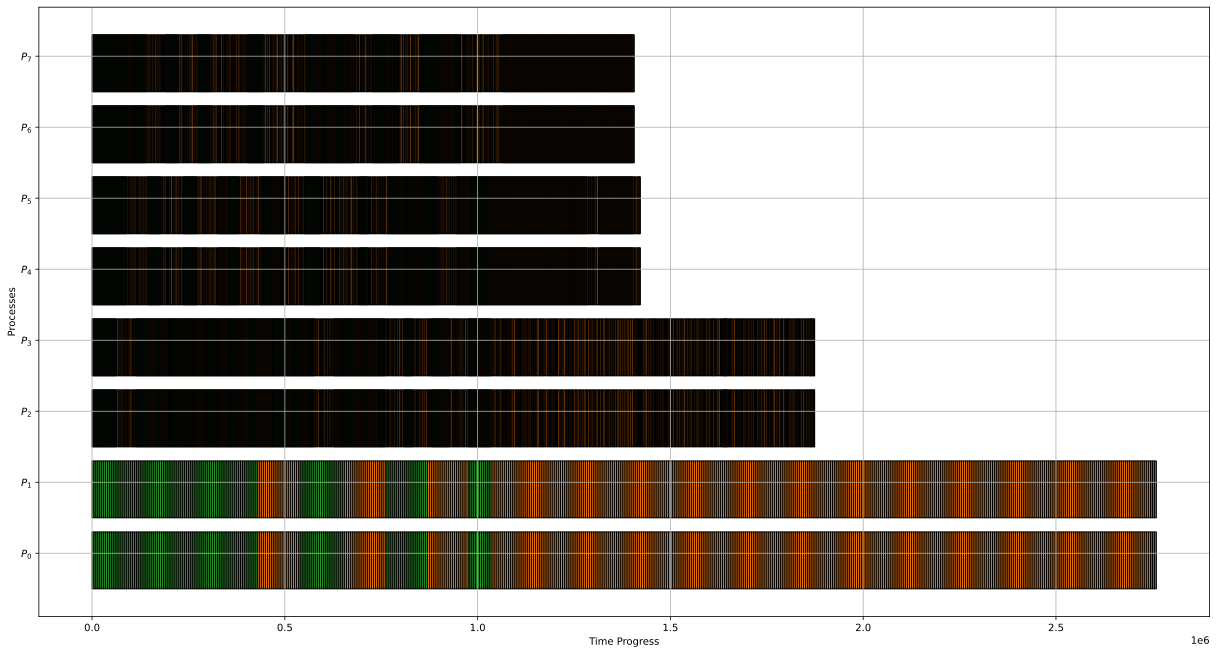
\includegraphics[scale=0.36]{./pictures/perf_analysis_model/perf_model_simulate_react_lb_1000_tasks_per_rank.pdf}
	\caption{An example simulation run with reactive load balancing in the scenario of $8$ processes, $1000$ tasks/process.}
	\label{fig:react_lb_simulation_1000_tasks_per_rank_example}
\end{figure}

Following the time steps and actions simulated for Scenario $1$, the module \texttt{Profiler} of our simulator can record the information, such as when tasks are queued and started execution, migration, termination, to profile the behavior of reactive load balancing. Typically, Figure \ref{fig:react_lb_simulation_1000_tasks_per_rank_example} depicts the profiled task execution over time progress by the simulator. The x-axis indicates time progress, while the y-axis indicates $8$ processes in this simulation scenario. We configure $8000$ tasks in total and $1000$ tasks/process as a given distribution. Process $P_{0}$ and process $P_{1}$ are the slowdown processes. With the given scale of $5 \times$ slower than normal, one task is executed in $5$ seconds. Without load balancing, the total load of process $P_{0}$ and $P_{1}$ would be $5000$s. Through applying reactive load balancing, we can see that the completion time is reduced to around $2700$s.\\

In Figure \ref{fig:react_lb_simulation_1000_tasks_per_rank_example}, a range of ``green'' slots indicates local task execution, while ``orange'' indicates remote task execution. Such an example simulator run, we simply configure the overhead information, consisting of:
\begin{itemize}
	\item Balancing operation overhead (named $O_{\text{balancing}}$): $20$ms occupied $2\%$ of task execution time unit. This means a task is executed in $1$s ($1000$ms), then balancing operations at once take $20$ms. As mentioned in Subsection \ref{subsec:discrete_time_model}, $O_{\text{balancing}}$ accounts for the time of monitoring ($m_{i}(t, t+\Delta t)$) and exchaning load information ($b_{i}(t - \lambda)$).
	\item Task migration overhead (represented by delay time $d$): $10$ms occupied $1\%$ of the task execution time unit.
\end{itemize}

As we can see in Figure \ref{fig:react_lb_simulation_1000_tasks_per_rank_example}, reactive task migration is sometimes incorrect because process $P_{0}$ and $P_{1}$ are known as overloaded processes but they still receive remote tasks. This also happens in a real execution with certain cases of high imbalance alongside many tasks per process and small execution time per task In Figure \ref{fig:react_lb_simulation_1000_tasks_per_rank_example} with the processes $P_{2}$, $...$, $P_{7}$, the area of local tasks is tight and overlaps together; therefore, we might not see clear local task execution. With process $P_{0}$ and $P_{1}$, the area of remote tasks is marked such incorrect task offloading at several time slots.\\

The following subsection provides further details about the evaluation of our simulator. We intend to show the impact between balancing operation overhead and task migration overhead. Notably, we address why reactive load balancing is late at runtime in distributed memory systems.

% We have these constraints to declaring imbalance context based on the number of involved processes ($P$), tasks ($T$), the scale of slowdowns such as $20\%$, $30\%$, or $50\%$, ..., then the number of processes being slow. The last input is the execution rate which denotes how many tasks can be done per time unit, or we can say how the throughput of execution (tasks/time unit) is.\\

% Below the \texttt{Simulation Engine spec.} region is an iteraction region, including \texttt{Balancer} and \texttt{Migrator}. Each time clocking, the balancer will check the queue's status for imbalance ratio ($R_{imb}$). If $R_{imb}$ meets the requirement of offloading tasks, it will signal \texttt{Migrator} for further actions to offloading tasks. Additionally, there is the second interaction region named \texttt{Profiler}. Before a time clock is closed, we can trigger the profiler to trace and record data for visualizing the simulation of our execution with dynamic load balancing. As we can see, the diagram extends the design in Figure \ref{fig:react_lb_simulator} to a communication diagram in more detail. Following the action arrows, we can determine the working flow from the points of simulation view. For example, after getting the imbalance context, we start with \texttt{queue\_setup()}, and \texttt{Clocking} is managed to proceed. Then, the behavior contineou by checking the queues (\texttt{check\_queue()}), ... until the termination of a loop (at \texttt{4.} \texttt{increase} \texttt{\_clock()}).\\

\subsection{Simulator Evaluation}
\label{subsec:Simulator-Evaluation}

\subsubsection{Example without load balancing}
\label{subsubsec:eval-sim-example-no-lb}

The simulation scenario in this subsection is similar to the previous example of Figure \ref{fig:react_lb_simulation_1000_tasks_per_rank_example}. However, we reduce the total number of tasks to reduce simulation time, where each process holds $100$ tasks. The imbalance ratio is also configured $R_{imb} = 1.5$, $P = 8$ processes, and below is an input sample for configuring the simulator.

\begin{lstlisting}[language=Python, caption={Input sample for the baseline simulation.}, label={lst:sim_input_sample}]
	num_process: 8
	num_tasks:   800
	slowdown:    0.2 # the scale of slowdown
	num_sld_processes: 2 # the number of slowed processes
	bandwidth: 1485 MB/s # bandwidth value for calculating delay
	exe_rate: 1.0 task/s # the execution rate
\end{lstlisting}
\hfill

\begin{figure}[t]
  \centering
  \includegraphics[scale=0.65]{./pictures/poc_implementation/poc_visualize_baseline_case_8_processes.pdf}
	\caption{Visualization of the baseline simulation without load balancing.}
	\label{fig:simulator_baseline_case}
\end{figure}

This input is used to simulate the baseline without load balancing. Technically, module \texttt{Balancer} is deactivated in this case. Therefore, there are no values for balancing operation overhead and task migration overhead. With time steps in milliseconds (ms), the clock is counted one by one at a time. In normal processes, the execution rate is $1.0$ task/s, and the total load value of each is ideally $100$s. In slowdown processes, the execution rate is $0.2$, where we simply set process $P_{0}$ and $P_{1}$ as the slow processes. Executing each task in process $P_{0}$ and $P_{1}$ takes $5$s. The completion time without load balancing is $500$s in total. Figure \ref{fig:simulator_baseline_case} shows the simulated baseline. The x- and y-axis also point to the time progress and the load-value bars of $8$ processes. Green boxes denote the executed tasks that are clearly seen at process $P_{0}$ and process $P_{1}$. The load values on other processes are smaller compared to process $P_{0}$ and $P_{1}$ due to many overlapped tasks. Hence, we might see task execution on their sides black (not clearly green as expected).\\

The following is a detailed statistic output from our simulator (Listing \ref{lst:sim_output_sample}). First, the configuration information (under the block \texttt{Configuration}) is summarized. Second, under the block \texttt{Executed Tasks}, the output summarizes the number of local and remote tasks executed on each process. Then, the blocks \texttt{Total Load} and \texttt{Statistic} summarize the total load values of processes and the corresponding maximum, minimum, average load values, resulting in the imbalance ratio. Overall, the detailed output and profiled data can be directed to a \texttt{csv}-format file.

\begin{lstlisting}[language=Python, caption={The output of the baseline simulation.}, label={lst:sim_output_sample}]
-------------------------------------------
Configuration
-------------------------------------------
   + num. processes:     8
   + num. tasks:       800
   + slowdown:         0.2
   + num. sld.procs:     2
   + bandwidth:      1485.0 (MB/s)
   + exe_rate:         1.0 (task/s)
-------------------------------------------

-------------------------------------------
Summary: Executed Tasks
-------------------------------------------
	 + P[0]: num.local_tasks=  100, num.remote_tasks=    0
	 + P[1]: num.local_tasks=  100, num.remote_tasks=    0
	 + P[2]: num.local_tasks=  100, num.remote_tasks=    0
	 + P[3]: num.local_tasks=  100, num.remote_tasks=    0
	 + P[4]: num.local_tasks=  100, num.remote_tasks=    0
	 + P[5]: num.local_tasks=  100, num.remote_tasks=    0
	 + P[6]: num.local_tasks=  100, num.remote_tasks=    0
	 + P[7]: num.local_tasks=  100, num.remote_tasks=    0
-------------------------------------------

-------------------------------------------
Summary: Total Load
-------------------------------------------
   + P[0]: local_load= 500.00(s), remot_load=   0.00(s)
   + P[1]: local_load= 500.00(s), remot_load=   0.00(s)
   + P[2]: local_load= 100.00(s), remot_load=   0.00(s)
   + P[3]: local_load= 100.00(s), remot_load=   0.00(s)
   + P[4]: local_load= 100.00(s), remot_load=   0.00(s)
   + P[5]: local_load= 100.00(s), remot_load=   0.00(s)
   + P[6]: local_load= 100.00(s), remot_load=   0.00(s)
   + P[7]: local_load= 100.00(s), remot_load=   0.00(s)
-------------------------------------------

-------------------------------------------
Statistic
-------------------------------------------
max. load:   500.0
min. load:   100.0
avg. load:   200.0
R_imb:         1.5
sum. overloaded_load:    600.0
sum. underloaded_load:   600.0
-------------------------------------------
Write profiled queue data to: ./poc_visualize_baseline_case_8_procs_output.csv
-------------------------------------------
\end{lstlisting}
\hfill

\subsubsection{Example with reactive load balancing}
\label{subsubsec:eval-sim-example-reactlb}

In the case of applying reactive load balancing, we activate \texttt{Balancer} and configure the values for balancing operation overhead and task migration overhead. With a simulation trial, we initially set the balancing overhead, $O_{\text{balancing}} = 1.0$ms, and delay time, $d=1.0$ms. Compared to the execution time unit of a task in second, we highlight that balancing overhead and delay time occupy $0.1\%$.\\

\begin{figure}[t]
  \centering
  \includegraphics[scale=0.65]{./pictures/poc_implementation/poc_visualize_reactlb_O1_d1_8_processes.pdf}
	\caption{Visualiztion of reactive load balancing case of simulation with $O_{\text{balancing}} = 1.0$ms and $d=1$ms.}
	\label{fig:simulator_reactlb_O1_d1_case}
\end{figure}

Figure \ref{fig:simulator_reactlb_O1_d1_case} shows the visualization of the simulation with reactive load balancing, where $O_{\text{balancing}} = 1.0$ms and $d = 1.0$ms. The x- and y-axis shows time progress and processes executing tasks, where ``green'' and ``orange'' slots indicate local can remote tasks. Overall, the completion time is reduced. The simulated operations of reactive task offloading with $O_{\text{balancing}}$ and $d$ are acted as follows.
\begin{itemize}
	\item Suppose at a time $t_{k}$, module \texttt{Balancer} detects an imbalance and tasks from process $P_{0}$ are then offloaded to process $P_{7}$ as an example. However, the tasks are proceeded in the queue for offloading at time $t_{k} + 1$ because of $O_{\text{balancing}} = 1.0$.
	\item Similarly, assuming tasks from process $P_{0}$ are decided to offload to process $P_{7}$ at $t_{k}$. However, these tasks arrive at process $P_{7}$ at time $t_{k} + 1$ because of $d = 1.0$.
\end{itemize}

In the simulator, module \texttt{Clocking} controls the ticking procedure of time steps. We can adjust this procedure to simulate the execution of dynamic load balancing similar to running in practice. Listing \ref{lst:sim_output_reactlb_O1_d1} shows the output sample of this simulated scenario. The output format is equivalent to Listing \ref{lst:sim_output_sample}, but we skip the part of \texttt{Configuration}. As a result, the summary under block \texttt{Executed Tasks} highlights the number of remote tasks from process $P_{2}$ to $P_{7}$. In response to the number of remote tasks, block \texttt{Total Load} indicates the total load values of remote tasks, proving that reactive load balancing works. In the end, the completion time is improved significantly $\approx 165.0$ms, and $R_{imb}$ is almost $0.0$.

\begin{lstlisting}[language=Python, caption={The simulation output of reactive load balancing with $O_{\text{balancing}} = 1.0$ms, $d=1$ms}, label={lst:sim_output_reactlb_O1_d1}]
-------------------------------------------
Configuration
-------------------------------------------
   ...
-------------------------------------------

-------------------------------------------
Summary: Executed Tasks
-------------------------------------------
	 + P[0]: num.local_tasks=   33, num.remote_tasks=    0
	 + P[1]: num.local_tasks=   33, num.remote_tasks=    0
	 + P[2]: num.local_tasks=   82, num.remote_tasks=   38
	 + P[3]: num.local_tasks=   82, num.remote_tasks=   38
	 + P[4]: num.local_tasks=   81, num.remote_tasks=   42
	 + P[5]: num.local_tasks=   81, num.remote_tasks=   42
	 + P[6]: num.local_tasks=   76, num.remote_tasks=   48
	 + P[7]: num.local_tasks=   76, num.remote_tasks=   48
-------------------------------------------
	
-------------------------------------------
Summary: Total Load
-------------------------------------------
   + P[0]: local_load= 165.00(s), remot_load=   0.00(s)
   + P[1]: local_load= 165.00(s), remot_load=   0.00(s)
   + P[2]: local_load=  82.00(s), remot_load=  72.50(s)
   + P[3]: local_load=  82.00(s), remot_load=  72.50(s)
   + P[4]: local_load=  81.00(s), remot_load=  75.00(s)
   + P[5]: local_load=  81.00(s), remot_load=  75.00(s)
   + P[6]: local_load=  76.00(s), remot_load=  81.00(s)
   + P[7]: local_load=  76.00(s), remot_load=  81.00(s)
-------------------------------------------

-------------------------------------------
Statistic:
-------------------------------------------
max. load:   165.0
min. load:   154.5
avg. load:   158.1
R_imb:         0.0
sum. overloaded_load:     13.8
sum. underloaded_load:    13.8
-------------------------------------------
Write profiled queue data to: ./profiled_queues_reactlb_O1_d1.csv
-------------------------------------------
\end{lstlisting}

\subsubsection{Experiments with the simulator}
\label{subsubsec:eval-sim-experiments-reactlb}

\begin{figure}[t]
\centering
\subfloat[Subfigure1][Reactive LB with $O_{\text{balancing}}$ $=2$ms and $d=2$ms]{
\includegraphics[scale=0.525]{./pictures/poc_implementation/poc_visualize_reactlb_O2_d2_8_processes.pdf}
\label{sfig:reactlb_O2_d2}}
\subfloat[Subfigure2][Reactive LB with $O_{\text{balancing}}$ $=5$ms and $d=2$ms]{
\includegraphics[scale=0.525]{./pictures/poc_implementation/poc_visualize_reactlb_O5_d2_8_processes.pdf}
\label{sfig:reactlb_O5_d2}}
\qquad
\subfloat[Subfigure3][Reactive LB with $O_{\text{balancing}}$ $=10$ms and $d=2$ms]{
\includegraphics[scale=0.525]{./pictures/poc_implementation/poc_visualize_reactlb_O10_d2_8_processes.pdf}
\label{sfig:reactlb_O10_d2}}
\subfloat[Subfigure4][Reactive LB with $O_{\text{balancing}}$ $=20$ms and $d=2$ms]{
\includegraphics[scale=0.525]{./pictures/poc_implementation/poc_visualize_reactlb_O20_d2_8_processes.pdf}
\label{sfig:reactlb_O20_d2}}
\caption{A visualization of reactive load balancing with increased balancing overhead and delay.}
\label{fig:simulator_reactlb_increased_Ovaried_d2}
\end{figure}

To see the effects of balancing overhead, we try to increase $O_{\text{balancing}}$ first from $2$, $5$, $10$, to $20$ms, corresponding to the occupation of $0.2\%$, $0.5\%$, $1.0\%$, $2.0\%$ over task execution time unit, while $d = 2$ is kept constantly. Figure \ref{fig:simulator_reactlb_increased_Ovaried_d2} shows these tests in the visualization of reactive load balancing (denoted by Reactive LB). Compared to the baseline (in Figure \ref{fig:simulator_baseline_case} on Page \pageref{fig:simulator_baseline_case}) and the initial imbalance scenario (in Figure \ref{fig:simulator_reactlb_O1_d1_case} on Page \pageref{fig:simulator_reactlb_O1_d1_case} with $O_{\text{balancing}}$ $=1$ms, $d=1$ms), Figure \ref{fig:simulator_reactlb_increased_Ovaried_d2} highlights the impact of balancing operation overhead. Not only delay time, load balancing operations in monitoring, exchanging load information/queue status, and calculating imbalance conditions can also significantly affect overall performance. $O_{\text{balancing}}$ is sensitive when almost all dynamic load balancing methods decide on many continuous actions and task migrations. For instance, the balancing decisions start getting worse when $O_{\text{balancing}}$ occupies $0.5\%$ over task execution time unit.\\

\begin{figure}[t]
\centering
\subfloat[Subfigure1][Reactive LB in that keep $O_{\text{balancing}}=2$ constantly and vary $d$]{
\includegraphics[scale=0.4]{./pictures/perf_analysis_model/perf_model_queue_decrease_delay_impact_OB2.pdf}
\label{sfig:reactlb_O2_dvaried}} \\

\subfloat[Subfigure2][Reactive LB in that keep $O_{\text{balancing}}=5$ constantly and vary $d$]{
\includegraphics[scale=0.4]{./pictures/perf_analysis_model/perf_model_queue_decrease_delay_impact_OB5.pdf}
\label{sfig:reactlb_O5_dvaried}} \\

\subfloat[Subfigure3][Reactive LB in that vary $O_{\text{balancing}}$ and keep $d=2$ constantly]{
\includegraphics[scale=0.4]{./pictures/perf_analysis_model/perf_model_queue_decrease_blancing_impact_d2.pdf}
\label{sfig:reactlb_Ovaried_d2}}

\caption{Evaluation of the queue length convergence when varying task migration overhead (delay) and balancing operation overhead.}
\label{fig:evaluation_Obalancing_effects}
\end{figure}

For another evaluation, we keep $O_{\text{balancing}}$ as a constant and vary $d$ to see the impact of task migration overhead, Figure \ref{fig:evaluation_Obalancing_effects} shows two experiments conducted, one in Figure \ref{sfig:reactlb_O2_dvaried} showing $O_{\text{balancing}}=2$ and $d$ is ranged from $0.1\%$ to $2\%$; one in Figure \ref{sfig:reactlb_O5_dvaried} showing $O_{\text{balancing}}=5$ and $d$ is ranged from $0.1\%$ to $2\%$. The imbalance scenario is stayed similar to the previous tests. In both figures, the x-axis indicates the progress of queues changed over time steps (in ms); the y-axis indicates the queue length as the number of remaining tasks over time steps.\\

Generally, all the queues are converged into $0$ at the end after the execution is finished. However, the slope of different queue lines might be different because some processes are slowed down and execute tasks slower. Note that these experiments with the simulator are applied reactive load balancing, and the final results show the load balancing performance. Typically, the slope in these figures represents how efficient the performance is. The last queue converged at shorter time steps determines a better performance. The balancing operation overhead is still trivial with $O_{\text{balancing}}=2$. We can see that increasing $d$ does not affect the convergence speed much. However, with $O_{\text{balancing}}=5$, delay $d$ here is more sensitive, and the convergence of queues gets impacted. Following this, if we compare with the experiments visualized in Figure \ref{fig:simulator_reactlb_increased_Ovaried_d2} (on Page \pageref{fig:simulator_reactlb_increased_Ovaried_d2}) when $d$ is constant and $O_{\text{balancing}}$ is varied, Figure \ref{sfig:reactlb_Ovaried_d2} emphasizes in detail these scenarios with the convergence of queue lengths. For a slightly change of $O_{\text{balancing}}$, the load balancing performance is significantly affected.



\section{Towards Proactive Idea in Dynamic Load Balancing and Co-scheduling Tasks}
\label{sec:Idea-Proactive-LB}
\index{PerfModel!A Proactive Idea for Load Balancing}

The previous section highlights that task migration overhead in distributed memory systems is not the only primary influence factor. Instead, balancing operation overhead can also affect our performance. The balancing operations consist of monitoring queue information or status, calculating imbalance, exchanging status information, and making decisions on task migration. The overhead of each operation might be small and trivial. However, when they are performed numerously and continuously, the decisions of task migration can be significantly impacted. Eventually, the performance of load balancing is affected overall.\\

This subsection emphasizes three representative pillars that lead to wrong decision-making for reactive load balancing in particular and dynamic load balancing in general. Figure \ref{fig:three_pillars_reactlb} shows these pillars from left to right, including:
\begin{itemize}
	\item The first pillar implies the factors of imbalance reason (in our context, slowdown is mentioned and denoted by $S_{P}$) and imbalance level ($R_{imb}$).
	\item The second pillar is related to the overhead of load monitoring ($m$) and information exchanging ($b$).
	\item The third pillar is the overhead of task offloading, indicating the delay time ($d$) when tasks are migrated.
\end{itemize}

\begin{figure}[t]
  \centering
  \includegraphics[scale=0.55]{./pictures/perf_analysis_model/perf_three_pillars_of_react_lb.pdf}
	\caption{Three pillars of factors might challenge reactive load balancing.}
	\label{fig:three_pillars_reactlb}
\end{figure}

Concretely, the first pillar implies imbalance context related to performance slowdown, leading to high or low imbalance levels. The second pillar is overhead in the middle, revolving around balancing operations. At runtime, all dynamic load balancing methods perform seemingly random operations before a task can be migrated. The last pillar is about overhead and decision-making for task offloading as well as task migration. If the second pillar takes a small overhead, then decisions in the third pillar can be made faster. When tasks are decided to migrate, the main overhead is delay time $d$, which $d$ is large or small, depending on the data size of tasks, latency, and network bandwidth. We describe the interaction between these pillars as follows.
\begin{itemize}
	\item If $R_{imb}$ is high, the imbalance condition might be detected in high frequency. Then, task offloading decisions are made many times.
	\item To know how many tasks and where to offload tasks, there are different ways to make decisions associated with the first pillar.
	\begin{itemize}
		\item For safety, exactly one task should be moved at one point in time. However, this might lead to many monitoring, checking, and exchanging load information operations. Simultaneously, the big enough values of $d$ can make these points challenging because it can take time to finish the exchanging operations before a task is decided for migration.
		\item To reduce the number of migration procedures, several tasks can be moved at once. However, deciding how many tasks are appropriate without prior knowledge is difficult.
	\end{itemize}
\end{itemize}

We can see that ``reactive'' load balancing implies taking actions reactively based on the most current status. This also means that we cannot plan to decide how many tasks should be migrated at a time adaptively. Besides, there is no information about which process could be a potential victim. When balancing operation and task migration produce a certain overhead, the decisions of reactive load balancing can be late and incorrect.\\

In general, we highlight that the challenge of dynamic load balancing is to obtain prior knowledge about load information. Assuming that we can predict load information or generate knowledge about load information at runtime, we can drive load balancing better. This thesis motivates an idea: How can we perform load balancing more proactively at runtime? ``Proactive'' implies that we can calculate how bad the imbalance is at a current state and how many tasks should be migrated at once. Consequently, we propose a proactive load balancing approach that enables to characterize task execution, learn load information, and predict imbalance. This is considered a better prognostication compared to the reactive load balancing approach. From idea to practice, our proactive approach is developed by the following technical questions:
\begin{itemize}
	\item Can we use a dedicated thread to obtain load values at runtime?
	\item Can we leverage the profiled information of several first iterations (or previous iterations) to generate the load knowledge?
	\item Can we change from reactive to more proactive task offloading between iterations?
\end{itemize}

For most of the use cases in HPC, iterative applications or simulation frameworks can benefit from our approach. Their behaviors are divided into multiple execution phases (so-called iterations). With a large simulation use case, a program can be run with many iterations, and an adaptive approach for load balancing is essential. Therefore, our proactive idea can be relevant to make load balancing more adaptive. The following chapter will show in detail how we design the idea.

% Taking a look at the condition for task offloading, it relies on setting an imbalance threshold and the availability of tasks at a time.

%\section{Related Models for Work Stealing}
\label{sec:Refer-Model-WS}
\index{PerfModel!Related Models for Work Stealing}

\begin{figure}[t]
  \centering
  \includegraphics[scale=0.8]{./pictures/perf_analysis_model/perf_analysis_related_model_without_latency.pdf}
	\caption{An illustration of work-stealing without latency concern.}
	\label{fig:perfmodel_relatedmodelwithoutlatency}
\end{figure}

As mentioned, we illustrate again an example of work stealing behaviors in Figure \ref{fig:perfmodel_relatedmodelwithoutlatency}, but this case is without latency concern. This model is commonly known in shared memory systems. The idea is that idle processes will try to steal tasks from other busy processes. Communication is assumed very fast to send and receive tasks immediately. As we can see, the x-axis shows the execution progress by time, along with four processes indexed from 0 to 3. The triangles represent stealing operations at a time. This is an ideal case for load balancing when the time to send and receive tasks is almost instantaneous.\\

To demystify the related models and our proposed model in the next sections, we attempt to merge some related terminologies as well as notations so that they are consistent in this thesis. For example, the total number of tasks is reused and named $T$, distributed on $P$ processes before execution. Table \ref{tab:mapped_notation_table} will show in detail the other related notations. Such the concern, each process in $P$ after a given distribution of $T$ tasks will hold a subset of $T_{i}$ tasks. In some related works, they used $w_{i}$ to indicate the number of tasks at process $i$  \cite{tchiboukdjian2013decentralized}. Thereby, we try to make it consistent with us by using $T_{i}$ as the number of tasks in process $i$. In the following sections, there might be some additional terms about the queue information, and $Q_{i}$ is used to denote the queue status, and they still refer to the values of the number of tasks. Mapping them to the time progress, this may have the field of time $(t)$ following. For instance, $T_{i}(t)$ means the number of tasks in process $i$ at time $t$, or $T(t)$ without $i$ means the total number of tasks (including all processes) at time $t$. The text might re-mention these notations in some specific paragraphs when we want to show further explanation.\\

\begin{table}[t]
\centering
\begin{tabular}{|l|p{2cm}|p{5cm}|p{4.5cm}|}
\hline
\textbf{No.} & \textbf{Notations} & \textbf{Description} & \textbf{Note}        \\ \hline
1  & $T$          & the number of tasks indexed $\left \{0,...,(T-1) \right \}$ & In some other related works, people used $W$ instead of $T$   \\ \hline
2  & $P$					& the number of processes, $\left \{0,...,(P-1) \right \}$    & Other works might use $m$ identical processors instead of $P$ \\ \hline
3  & $T_{i}$			& the set of assigned tasks in Process $i$                    & Other works might use $w_{i}$ instead of $T_{i}$              \\ \hline
4  & $L_{i}$			& the total load of Process $i$                               &                                             \\ \hline
5  & $w_{i}$			& the wallclock execution time of a task, i.e., task $i$      &                                             \\ \hline
6  & $W_{i}$ 			& the wallclock execution time of Process $i$                 &                                             \\ \hline
7  & $S_{P_{i}}$	& processing speed (performance model) of Process $i$         &                                             \\ \hline
8  & $Slow_{i}$		& slowdown coefficient of Process $i$ at runtime              &                                             \\ \hline
9  & $W_{par}$		& the total wallclock execution time (makespan)               & Also called completion time ($C$)           \\ \hline
10 & $R_{imb}$		& imbalance ratio                                             &                                             \\ \hline
11 & $\lambda$		& communication or network latency                            &                                             \\ \hline
12 & $d$					& delay or transmission time                                  &                                             \\ \hline
13 & $B$					& network bandwidth                                           &                                             \\ \hline
14 & $O_{ij}(t)$	& the number of offloaded tasks from Process $i$ to $j$       & The authors in \cite{tchiboukdjian2010tighter} used $R(t)$ as the number of task requests in global after time $t$ \\ \hline
\end{tabular}
\caption{Used notations in the thesis comparing to the notations from related works.}
\label{tab:mapped_notation_table}
\end{table}

The main purpose of performance modeling is to show an upper bound of balancing efficiency with how many tasks can be migrated. Extended from an original work \cite{Blumofe1999OriginWS}, Tchiboukdjian et al. have proposed a good model for work-stealing without latency since 2010 \cite{tchiboukdjian2010tighter} \cite{tchiboukdjian2013decentralized}. In this section, we attempt to summarize their reference models. The first is mentioned as work stealing model without communication latency \cite{tchiboukdjian2010tighter} \cite{tchiboukdjian2013decentralized}. The second is timely analyzed by \cite{gast2021analysis} in 2021, also work stealing but with latency variable.\\

In \cite{tchiboukdjian2013decentralized}, Tchiboukdjian et al. considered a parallel platform with $P$ processes. At time $t$, $T_{i}(t)$ represents the amount of works\footnote{At this point, works are considered as tasks in our context. Therefore, they might be used interchangeably.} on process $i$. Compared to $t=0$, $T_{i}(t)$ will be decreased by time progress. For example, at $t=0$ the workload is just distributed on each process, $T_{i}(t_{0}) = 100$ means holding 100 tasks before running. Then, at $t=10$ assume that 10 tasks have been done on process $i$, and $T_{i}(t_{10})$ would be $90$ such the remaining tasks. We can take Figure \ref{fig:perfmodel_relatedmodelwithoutlatency} as an example, at $t=10$ process $3$ has done 10 tasks and its queue remains 90 tasks, $T_{0}(t_{10}) = 90$. In constract, process $2$ is faster and it has done all tasks at $t=10$, therefore, $T_{2}(t_{10}) = 0$.\\

Therefore, the execution behavior will be simplified as follows,
\begin{itemize}
	\item when $T_{i}(t) > 0$, processor $i$ is active and execute tasks, $T_{i}(t+1) \leq T_{i}(t)$.
	\item when $T_{i}(t) = 0$, processor $i$ is idle and intends to steal tasks from a random processor $j$.
\end{itemize}

\noindent \textbf{A Tight Analysis of Work Stealing \cite{tchiboukdjian2010tighter,tchiboukdjian2013decentralized}}\\

If work stealing is applied, some tasks are moved around, then $T_{i}(t)$ will increase or decrease, depending on how many steal requests and tasks are performed at a time. Tchiboukdjian et al. \cite{tchiboukdjian2010tighter} \cite{tchiboukdjian2013decentralized} assumed that between time $t$ and $t+1$, there are $P - \alpha(t)$ steal requests, $P$ is the total number of processes and $\alpha(t)$ denotes the number of active processes, $\alpha(t) \in [0, m]$. When $\alpha(t)=0$, it means all queues are empty as well as the execution is complete. Corresponding to the sucess steal requests, process $j$ will transfer an amount of work to $i$ and $T_{i}(t+1) + T_{j}(t+1) \leq T_{j}(t)$. Similar to when $\alpha(t)=0$, the execution will terminate if $\forall i \in P, T_{i}(t) = 0$. At time $t$, the total number of tasks on all processes is denoted by $T(t) = \sum_{i=1}^{P}T_{i}(t)$. After that, process $2$ will steal some tasks from the others to help share the load. The triangle shows stealing operations, and there is obviously stealing overhead in practice. However, we show this related model with an assumption about no latency, in which the use cases might be considered in shared memory.\\

In the baseline without work-stealing, the total execution time depends on the process with a maximum load, $C_{max} = max_{i \in P} T_i(t_0)$, so-called makespan or critical path. When we use work stealing, $C_{max}$ can be reduced. Therefore, the main question of work stealing model is:
\begin{shaded}
	\noindent What is the upper bound of makespan when work stealing is applied?
\end{shaded}

The work has proposed a potential function $\Phi (t)$ to model the performance of work stealing through studying the potential decrease. Assuming that tasks are unit independent, $\Phi (t)$ is defined by
\begin{equation} \label{eq:phi_defi}
	\Phi(t) = \sum_{i=1}^{P} (T_{i}(t) - \frac{T(t)}{P})^{2} = \sum_{i=1}^{P} T_{i}(t)^{2} - \frac{T(t)^2}{P}
\end{equation}
where, the potential represents the load unbalance of execution. For example, as expected at time $t$ the average load among $P$ processes is $\frac{T(t)}{P}$. Then, if we sum the difference values between each process's load value at $t$ and the average value, the result shows how much load difference is. \\

Therefore, the decrease of $\Phi (t)$ depends on the number of steal requests and execution scenario. The above has mentioned an estimated formular for the number of steal requests ($P - \alpha(t)$). $\alpha(t)$ is a complicated random process that chooses the number of active processors at each step. Such an expectation in work-stealing, the more work requests it creates, the more the potential will decrease. The performance analysis model is performed in three steps:
\begin{enumerate}
	\item Define $\Phi (t)$.
	\item Compute the expected decrease of $\Phi (t)$ between step $t$ and $t+1$, $\Delta \Phi (t) \overset{def}{=} \Phi (t) - \Phi (t+1)$. However, at a specific time $t$, how can we estimate the decrease? To this end, the authors define another term, named $\delta_{i}^{k}(t)$, to compute the expected decrease,
	\begin{equation} \label{eq:expect_decrease}
		\sum_{i=1}^{P} \sum_{k=0}^{P-1} E [\delta_{i}^{k}|i\ \textrm{receives}\ k\ \textrm{requests}]P\left \{ i\ \textrm{receives}\ k\ \textrm{requests} \right \}
	\end{equation}
	
	, where the first sum goes through all $P$ processes and the second sum goes from $0$ to $(P-2)$ as the maximum requests a process can get at a time. $E[X|Y]$ denotes the expectation of $X$ knowing $Y$. Applying this to the example in Figure \ref{fig:perfmodel_relatedmodelwithlatency} we have
	
	\begin{equation}
		E[\Delta \Phi (t)] = \sum_{i=0}^{3} \sum_{k=0}^{3} E [\delta_{i}^{k}|i\ \textrm{receives}\ k\ \textrm{requests}]P\left \{ i\ \textrm{receives}\ k \textrm{requests} \right \}
	\end{equation}

	Following that, the authors showed that there exists a function called $h(\alpha) \in (0;1]$ such that $E[\Delta \Phi (t)|\Phi (t) = \Phi,\alpha(t) = \alpha] \geq h(\alpha) \Phi$.
	
	\item This work obtained a bound on the expected number of steal requests $E[R]$ ($R$ is the number of steal requests), and the expected makespan $E[C_{max}]$ can be further obtained from $E[R]$.
\end{enumerate}

This work concluded that the expected number of steal requests $R$ until $\Phi(t) \leq 1$ is bounded by $E[R] \leq \lambda \cdot P \cdot log_{2} \Phi(0)$, where $\lambda$ in this case is $max_{1 \leq \alpha \leq P-1} \frac{P-\alpha}{-P \cdot log_{2}(1-h(\alpha))}$ and $\Phi(0)$ is the potential at $t=0$. At the end, the expected value of $C_{max}$ will be bounded by 
\begin{equation}
	E[C_{max}] \leq \frac{T}{P} + \frac{2}{1-\log_{2}(1+\frac{1}{\epsilon})} \log_{2}W + 1
\end{equation}

Before \cite{tchiboukdjian2010tighter,tchiboukdjian2013decentralized}, some previous works also attempted to find an upper bound. One of the original studies from Blumofe and Leiserson \cite{Blumofe1999OriginWS} showed that the efficiency of work-stealing is bounded by $E(C_{max}) \leq \frac{T}{P} + O(D)$, where $D$ is the length of the critical path in the case of dependent tasks (represented as a graph). The analysis is further improved by \cite{arora2001thread} using potential functions. The authors used an amortization argument based on a potential function that decreases as the work-stealing algorithm processes. The idea is to divide the execution into phases and show that the potential decreases by at least a constant fraction with a constant probability. For the case of varying the speed of $P$ processors or heterogeneous processors, Bender and Rabin \cite{bender2002online} provided a new analysis of an old scheduling algorithm called \textit{maximum utilization scheduler}. The authors showed a given context for $P$ processors with speed $\pi_{i}$ steps/time. These studies are constrained in a context of only one source of tasks that could not easily model the basic case of independent tasks, and communication overhead is not explicitly counted.\\

\noindent \textbf{A Tighter Analysis of Work Stealing with Latency \cite{gast2021analysis}} \\

For modeling with communication latency, people are rarely concerned explicitly in work-stealing models. In 2021, Nicolas Gast et al. \cite{gast2021analysis} proposed a new analysis model on how communication latency impacts stealing operations in terms of task-parallel applications. The model has been created for distributed memory clusters with $P$ identical processors. Latency value is denoted by $\lambda$. The authors inherited from their previous work \cite{tchiboukdjian2013decentralized} and aimed at an upper bound for the expected makespan.\\

We investigate this related work in more detail which motivates us to propose a new model. From one of the previous studies \cite{tchiboukdjian2013decentralized}, the authors also make a consistent assumption about work-stealing algorithms in general:
\begin{itemize}
	\item The total number of processes is defined as $P$ identical processors.
	\item $T_{i}(t)$ denotes the amount of tasks on processor $i$ at time $t$, and the total tasks at $t$ would be $T(t) = \sum_{i=1}^{P}T_{i}(t)$. 
	\item A task corresponds to one unit of execution time.
	\item Latency: all communication take $\lambda \in N$ time unit.
	\item Single Task Transfer: a processor can send some tasks to at most one processor at a time.
	\item Steal Threshold: if the victim has less than $\lambda$ task units to execute, the stealing request will be failed.
	\item Task to be stolen: the victim sends to the thief half of its tasks at a time. For example, the total tasks of process $i$ at time $t$ is $T_{i}(t) = \frac{T_{i}(t-1) - 1}{2}$.
\end{itemize}

\begin{figure}[t]
  \centering
  \includegraphics[scale=0.8]{./pictures/perf_analysis_model/perf_analysis_related_model_with_latency.pdf}
	\caption{An illustration of work-stealing with latency effect.}
	\label{fig:perfmodel_relatedmodelwithlatency}
\end{figure}

Figure \ref{fig:perfmodel_relatedmodelwithlatency} demonstrates a scenario of work stealing with latency. The x-axis represents the time progress of execution with four involved processes. Process $2$ is assumed idle and sends a steal request to process $3$. Since process $3$ accepts, task is sent from $3$ to $2$. We name $\lambda$ as the latency, and one stealing action takes a round-trip time $2\lambda$. This occurs similarly between process $1$ and $0$.\\

As the round-trip time of $2\lambda$ and the total amount of tasks $T$ on $P$ processes, we can drive to a straightforward bound of makespan as \ref{eq:straight_cmax}.
\begin{equation} \label{eq:straight_cmax}
\begin{split}
	P \cdot & C_{max} \leq T + 2\lambda \cdot \#{\textrm{task requests}} \\
	\Leftrightarrow \ & C_{max} \leq \frac{T}{P} + 2\lambda \cdot \frac{\#{\textrm{task requests}}}{P}
\end{split}
\end{equation}

However, to be closer to an optimal bound, this work approached a potential function bounding on the number of work-stealing requests\footnote{Work-stealing requests mean the number of requests for stealing tasks in our context. Therefore, it is also called $\#{\textrm{task requests}}$ shown in Equation \ref{eq:straight_cmax} or steal requests}. The authors reconsidered the time division as periods of duration $\lambda$ to analyze the impact of latency. To not abuse notations, we use $T_{i}(k)$ and $s_{i}(k)$ to denote the current number of tasks and the number of stolen tasks from process $i$ at time $k$; then the quantities will be $T_{i}(k\lambda)$, $s_{i}(k\lambda)$. In the interval $(\lambda (k-1), \lambda k]$, the total number of incoming work-stealing requests is defined by $r(k) = \sum_{i=1}^{\lambda} R((k-1)\lambda + i)$, where $0 \leq r(k) \geq P$. The probability, that a process receives $\geq 1$ requests in the interval $(\lambda (k-1), \lambda k]$, is $q(r(k))$.\\

Nicolas Gast et al. \cite{gast2021analysis} showed the analysis of the potential decrease, which is defined in Equation \ref{eq:potfunc_latency} at time-step $k\lambda$.
\begin{equation} \label{eq:potfunc_latency}
\begin{split}
	\Phi(k) = 1 + \frac{1}{\lambda^2} \sum_{i=1}^{P} (T_{i}(k)^2 + 2s_{i}(k)^2)
\end{split}
\end{equation}

where, $\Phi(k)$ gets through all processes $\in P$, $T_{i}(k)$ and $s_{i}(k)$ represents the number of remaining tasks as well as the number of stolen tasks in process $i$ at time $k$. Let $\Phi(0)$ be the potential at time $t_{0}$ and $\tau$ be the first time step at which the potential reaches $1$. Then, the authors proved that the number of incoming steal requests until $\tau$, $R = \sum_{k=0}^{\tau = 1} r(k)$ satisfies:
\begin{equation} \label{eq:exp_prob_R_latency}
\begin{split}
	& E[R] \leq P \gamma \log_{2} \Phi(0) \\
	& \mathbb{P}[R \leq P \gamma (\log_{2} \Phi(0) + x)] \leq 2^{-x}
\end{split}
\end{equation}

In which, $E[R]$ is the expected number of total incoming steal requests and $\mathbb{P}$ indicates the probability when $R \leq P \gamma (\log_{2} \Phi(0) + x)$, and $\gamma$ is a constant such that $\gamma < 4.03$. Applying to $C_{max}$, the study concluded as Equation \ref{eq:exp_prob_Cmax_latency} shows.

\begin{equation} \label{eq:exp_prob_Cmax_latency}
\begin{split}
	& E[C_{max}] \leq \frac{T}{P} + 4\lambda\gamma\log_{2} \frac{P}{\lambda} + 2\lambda\gamma \\
	& \mathbb{P}[C_{max} \geq \frac{T}{P} + 4\lambda\gamma\log_{2} \frac{P}{\lambda} + x] \leq 2^{\frac{-x}{2\lambda\gamma}}
\end{split}
\end{equation}


\paragraph{Further discussion:}
The mentioned models above are relevant in terms of work stealing with or without latency. However, latency $\lambda$ is a constant, and the number of steal requests must contribute relatively, such as task execution time. These constraints might be limited by the cases in that task data sizes are different or transmission time considerably impacts the efficiency of stealing operations in practice. In contrast, this thesis analyzes the performance in a different direction. We introduce a proposed model associated with transmission time or delay time. The delay happens when tasks are migrated in distributed memory. First, the delay values depend on the size of task data in movement and the current status of interconnection, e.g., latency, bandwidth. Second, we figure out that this challenge can lead to other impacts on the decision time of taking stealing or balancing actions. This is a reason causing too late to balancing load in distributed memory. Next, we will discuss about a proposed model with delay time when tasks are migrated.


%\section{Model Evaluation}
\label{sec:Model-Evaluation}
\index{PerfModel!Model Evaluation}

This section introduces the experiments with our simulator to show when reactive load balancing can be late sometimes, leading to late decisions in offloading tasks. Our evaluation metric for this case is the decrease in queue length. Each process, in general, has a global queue of tasks. The execution threads per process get tasks from the queue for execution. Therefore, the queue length will be decreased toward $0$ over time steps, where the slowest process with queue length converging to $0$ determines the completion time of our application.\\

To be again consistent with the addressed example in the previous sections, we configure the simulation with $8$ ranks. Each rank here keeps $100$ tasks\footnote{To get the simulation results faster, we have reduced the number of tasks to $100$, compared to the one of $1000$ tasks in Figure \ref{fig:react_lb_simulation_1000_tasks_per_rank_example}.} at the beginning. Two of $8$ ranks are $5\times$ slower than normal, and the normal execution rate is $1$ tasks/second. This means the two slowdown ranks take $5$s to complete a task, while the others take $1$s for a task. In case of no load balancing, the completion time is $500$s because the two bottleneck ranks take $5$s/task. $R_{imb}$ is about $1.5$, clock timing is counted in one-by-one step, in which each step is $1$ms. Alongside, there are two variables varied in the experiments:
\begin{itemize}
	\item Balancing overhead ($O_{\text{balancing}}$): the values are varied such as $1, 2, 5, ...$, accounting for $0.1\%$, $0.2\%$, $0.5\%$ of overhead. 
	\item Delay time in task migration ($d$): its values are also varied such as $1, 2, 5, ...$, and also accounting for $0.1\%$, $0.2\%$, $0.5\%$ of overhead. 
\end{itemize}

\noindent \textbf{Vary delay ($d$) and keep balancing overhead ($O_{\text{balancing}}$) stable}\\
\noindent In this set of simulations, we vary the values of $d$ in a range of $[$ $0.1\%$, $0.2\%$, $0.5\%$, $1\%$, $2\%$ $]$, and keep the values of $O_{\text{balancing}}$ as a constant. \\

\begin{figure}[t]
  \centering
  \includegraphics[scale=0.45]{./pictures/perf_analysis_model/perf_model_queue_decrease_delay_impact_OB2.pdf}
	\caption{A simulation case to show the impact of delay time ($d$) with keeping the overhead of balancing operations as a constant of $0.2\%$.}
	\label{fig:react_lb_sim_delay_impact_Obal_2}
\end{figure}

Figure \ref{fig:react_lb_sim_delay_impact_Obal_2} shows a simulation experiment with the varied values of delay ($d$), while we keep the value of balancing overhead as a constant of $0.2\%$. Note that the percentage means the ratio with task runtime unit. Here the runtime is in seconds, and the values of $d$ or $O_{\text{balancing}}$ are in milliseconds. Therefore, $O_{\text{balancing}}$, in this case, takes $2$ms, occupying $0.2\%$ of a task runtime unit. As the figure shows, there are $8$ processes, where each line indicates the decrease or the convergence of its queue to $0$ over the execution time progress (on the x-axis). The y-axis shows the queue length values. At the very beginning, the queue length of all processes is the same, $100$ tasks. Following execution and reactive load balancing, they tend to decrease steadily but might sometimes increase if receiving tasks from a remote process. There are five plots from left to right, illustrating the simulation when $d$ is varied from $0.1\%$ to $2\%$. The time that the last process goes to $0$ also highlights the completion time. Figure \ref{fig:react_lb_sim_delay_impact_Obal_2} shows that the increasing values of $d$ do not highly change the completion time in this case. Such a baseline, if we do not apply any load balancing methods, the completion time will be $500k$. Therefore, the simulating case in Figure \ref{fig:react_lb_sim_delay_impact_Obal_2} shows that reactive load balancing is significantly useful.\\

\begin{figure}[t]
  \centering
  \includegraphics[scale=0.45]{./pictures/perf_analysis_model/perf_model_queue_decrease_delay_impact_OB5.pdf}
	\caption{A simulation case to show the impact of delay time ($d$) with keeping the overhead of balancing operations as a constant of $0.5\%$.}
	\label{fig:react_lb_sim_delay_impact_Obal_5}
\end{figure}

Next, we try to increase the balancing overhead a little more by $0.5\%$. Figure \ref{fig:react_lb_sim_delay_impact_Obal_5} shows the simulations with $O_{\text{balancing}}=5$. Some queues initially receive tasks from $P0$ and $P1$, for example, $P7$. This is why the $P7$ queue length is larger than $100$ tasks at that moment. In the end, the completion time is still slightly improved ($< 500$k ms) rather than the baseline. However, this simulating case shows that the overhead of balancing operations can greatly impact the time when task offloading is decided to take action. Even though the strategy of reactive load balancing can perform task migration earlier, it is still challenging during decision-making. In the next simulation scenarios, we keep $d$ as a constant and vary the value of $O_{\text{balancing}}$.\\

\noindent \textbf{Vary balancing overhead ($O_{\text{balancing}}$) and keep delay ($d$) stable}\\
\noindent In this set of simulations, we vary the values of $O_{\text{balancing}}$ in a range of $[$ $0.1\%$, $0.2\%$, $0.5\%$, $1\%$, $2\%$ $]$, and keep the values of $d$ as a constant.\\

\begin{figure}[t]
  \centering
  \includegraphics[scale=0.45]{./pictures/perf_analysis_model/perf_model_queue_decrease_blancing_impact_d2.pdf}
	\caption{A simulation case to show the impact of balancing-operations overhead ($O_{\text{balancing}}$) with keeping the delay time as a constant of $0.2\%$.}
	\label{fig:react_lb_sim_Obalancing_impact_d_2}
\end{figure}

Figure \ref{fig:react_lb_sim_Obalancing_impact_d_2} shows the simulation experiments with the varied values of $O_{\text{balancing}}$, while we keep $d$ as a constant of $2$ ms. As the results, the low overhead of $O_{\text{balancing}}$ is not a problem with load balancing. After $O_{\text{balancing}} \geq 0.5$, the performance get worse. In detail, the queue of $P1$ (one of the slowdown processes) converges to $0$ slow. Besides, it also get wrong task offloading. Instead of offloading tasks, it receives tasks from other processes when the offloading decision are performed incorrectly. There are two reasons for this:
\begin{itemize}
	\item Proceeding long before tasks are migrated: this means that slow processes have tried to offload as many tasks as possible at the beginning to fast processes, but it does not take immediately to proceed further for migration. Then, after a certain period, the queue of slow processes is less than the queue of fast processes, and tasks from the fast side are decided to offload to the slow side.
	\item Proceeding long before tasks are received: similar to proceed tasks for migrating, if the receiving sides proceed slowly, the tasks being on the offloading way are received late. Then, the monitored information of queues might not be correct, leading to wrong decision of task migration.
\end{itemize}

\begin{figure}[t]
  \centering
  \includegraphics[scale=0.45]{./pictures/perf_analysis_model/perf_model_queue_decrease_blancing_impact_d5.pdf}
	\caption{A simulation case to show the impact of balancing-operations overhead ($O_{\text{balancing}}$) with keeping the delay time as a constant of $0.5\%$.}
	\label{fig:react_lb_sim_Obalancing_impact_d_5}
\end{figure}

Therefore, Figure \ref{fig:react_lb_sim_Obalancing_impact_d_2} reveals that the case of $O_{\text{balancing}} = 1.0$ or $O_{\text{balancing}} = 2.0$ is even worse than the baseline, even the imbalance ratio can be slightly lower but the completion time is not better. This situation is more emphasized when we continue increasing the value of $d$ to $5$ ms. Figure \ref{fig:react_lb_sim_Obalancing_impact_d_5} demonstrates the results with $d = 5$. The trend of balancing-operations impact still keeps similar.\\

\noindent \textbf{Randomize delay ($d$) and balancing overhead ($O_{\text{balancing}}$)}\\
\noindent In this set of simulations, we randomize both values of $d$ and $O_{\text{balancing}}$ in the range of $[$ $0.1\%$, $0.2\%$, ..., $5\%$ $]$. Additionally, we perform the simulations as an iterative execution. This means that we repeat the simulation over iterations. Along with the randomized values of $d$ or $O_{\text{balancing}}$, each simulation iteration can have different values of them.

% Chapter \ref{ch:perfmodel}
% Our work looks at a higher level of task migration when the task data can be affected by transmission time or delay ($d$). The idea is to understand how impacts dynamic balancing operations under a certain imbalance level and a delay when tasks are migrated.
% $d$ at a time depends on latency and bandwidth. Transmission time or delay is the time of transmitting an entire message between two compute nodes. If there are no conflicts, the delay can be computed by $d(S) = \lambda + S/B$, where $S$ denotes the message size, $\lambda$ is the constant latency, and $B$ is the network bandwidth. Indeed, the message size depends on how tasks are simplified, which could be task argument or output data. Our model supports building a simulator, which gets the initial task distribution and related communication constraints as input.\\

%Delay is calculated by the latency and bandwidth at a period plus the size of migrated tasks. Hence, the delay time can more or less affect the load balance performance. In detail, we aim to clarify step by step the following ideas,
%\begin{itemize}
%	\item Analyze related models of work stealing with and without communication latency.
%	\item Introduce a proposed model with delay time in task migration. This model can be used to analyze work stealing and reactive task offloading.
%	\item Introduce a corresponding simulator to investigate the bound of these existing solutions and constraints as mentioned
%	\item Explain further the idea of proactive load balancing.
%\end{itemize}
\chapter{A Proactive Approach for Dynamic Load Balancing}
\label{ch:PADLB}
\index{PADLB!Proactive Approach for Load Balancing}
\chaptertoc
\noindent

This chapter discusses our proactive approach for dynamic load balancing. The goal is ``\textit{more information, better load balancing}''. Almost all static load balancing methods assume to have load information or related information to generate a cost model. Thereby, task migration and task distribution rely on prior knowledge to solve balancing. In dynamic load balancing, we do not rely on prior knowledge. Task migration is mainly based on the most current execution status at runtime, such as queue length and execution speed on each process. However, current status information is insufficient, implying that approaches like work stealing or reactive load balancing are seemingly based on speculation. Obviously, speculative balancing operations can be right or wrong for a given period.\\

\section{Overview}
\label{sec:PADLB-Overview}

In our proactive approach, we exploit influence factors related to execution status to predict and provide knowledge of task execution time. The knowledge based on load prediction helps to estimate the level of imbalance. We calculate the number of appropriate tasks and potential processes for task offloading. Benefiting from modern computer architectures and task-based programming models, the approach extends reactive load balancing by employing a dedicated thread for:

\begin{itemize}
	\item Supporting task and system characterization instead of only monitoring queue length.
	\item Using the characterization information to predict load values at runtime. Instead of missing the prior knowledge before running applications, we can generate new knowledge based on predicted load values, e.g., $w$, $L$.
	\item Adapting the prediction knowledge to guide task offloading. We calculate the load difference, the number of tasks, and potential process candidates for better offloading tasks.
\end{itemize}

Our approach is implemented towards a proactive scheme of load balancing, which facilitates different task offloading methods. To be intuitive, Figure \ref{fig:padlb_proact_scheme} shows how this scheme works. The x-coordinate again shows the time progress, while the y-coordinate shows process $P_{i}$ spawning two threads for executing tasks and one dedicated thread for performing load balancing. This thread fits today's modern computing architectures with the increasing number of cores, where one core can be left off to run the dedicated thread (denoted by $T_{comm}$). In practice, our scheme can be deployed through hybrid MPI+OpenMP, which is mostly exploited in various task-based parallel programming models.\\

\begin{figure}[t]
	\centering
	\includegraphics[scale=0.7]{./pictures/padlb_approach/padlb_proact_scheme.pdf}
	\caption{A proactive scheme for task offloading to solve dynamic load balancing in general.}
	\label{fig:padlb_proact_scheme}
\end{figure}

In Figure \ref{fig:padlb_proact_scheme}, we suppose that process $P_{i}$ contains two threads, $Thr_{0}$ and $Thr_{1}$, for executing tasks and one dedicated thread, $Tcomm_{i}$, for communication as well as proactive load balancing. Assuming the execution is iterative, which indicates $Iteration_{0}$, then $Iteration_{1}$, and so on. Different from reactive load balancing, $Tcomm_{i}$ in our approach is driven to perform:

\begin{itemize}
	\item Mainly keeping communication overlapped with computation.
	\item Characterizing task feature and system information along with the corresponding load values, such as $w$, $L$, core frequency, etc.
	\item Training a load prediction model at runtime.
	\item Offloading tasks proactively.
\end{itemize}

%\begin{figure}[t]
%  \centering
%  \includegraphics[scale=0.625]{./pictures/padlb_approach/padlb_three_branches_proact_strategies.pdf}
%	\caption{Three branches of task offloading strategies for proactive load balancing approach.}
%	\label{fig:three_branches_proact_strategies}
%\end{figure}

The above operations are what $Tcomm$ can perform separately from the other threads to facilitate load balancing. Furthermore, we can adapt these operations to specific application and system domains. The following sections show different task offloading methods based on our proactive balancing scheme. Specifically, we show two task offloading methods and one extension for co-scheduling tasks across multiple applications, including:

\begin{itemize}
	\item Method 1: feedback task offloading. We introduce method 1 in Section \ref{sec:PADLB-FeedbackLB}.
	\item Method 2: ML-based task offloading, where ``ML-based'' indicates a machine learning based model for online load prediction. Method 2 is described in Section \ref{sec:PADLB-MLbasedTaskOffload}
	\item Extension: co-scheduling tasks across multiple applications. We address this extension in Section \ref{sec:PADLB-CoschedulingTask}.
\end{itemize}

% The load value of each task or each process can be predicted on-the-fly. We use the prediction results to generate an adaptive algorithm for proactive task offloading.

% The extension from proactive load balancing: co-scheduling tasks across multiple applications. ``\textit{Co-scheduling}'' in load balancing also indicates migrating tasks from process to process. However, the scope of co-scheduling tasks here is across multiple applications, and task migration might be between different processes from different applications.

% After an iteration, it will share the information about the prediction, and each process can know the load status before a new iteration starts. Hence, each can plan to balance the load in advance.
 
% Section 4.0 different proactive strategies
%\section{More Information More Balancing Strategies}
\label{sec:PADLB-proactstrategies}
\index{PADLB!Proactive Strategies}

We focus on the perspective of ``\textit{more information more balancing strategies}''. Almost all static load balancing solutions have to assume that they know about load, the number of tasks, or specific information about applications beforehand. After that, the problem can be formulated and solved by optimal algorithms. The optimal solutions also resolve the output: how many tasks are partitioned and which processes/MPI ranks are. We do not have this information ready at runtime for dynamic balancing problems. What we can have is usually queue length status and execution speed. The balancing strategies have to decide which tasks are migrated, from which rank to which rank. We know little about the execution speed based on the number of remaining tasks in queues per rank or even per machine. All in all, the outcome of almost balancing solutions resolves around:
\begin{enumerate}
	\item Which process shares tasks to which process?
	\item And, how many tasks should be migrated at a time?
\end{enumerate}

Differing from work stealing or reactive load balancing, we introduce a new scheme to perform load balancing more proactive. The approach enables task characterization and load prediction at runtime. We then use the prediction to provide the missing knowledge about load at runtime and guide task offloading. Therefore, as mentioned above, we have partial load information to calculate well (1) and (2). Additionally, we can generate different strategies for task offloading.\\

The context in this work is not static or a master-slave scheduling model\footnote{Where, tasks are generated automatically or nested during execution}. Our context is a given distribution of tasks in distributed memory machines. The approach is described as the runtime scheme shown in Figure \ref{fig:padlb_proact_scheme}. We leave one core off to run a dedicated thread along with other execution threads\footnote{Or so-called main threads to execute tasks of the parallel program.}. From the runtime point of view, we can see that our programs are performed with multiple processes or MPI ranks in distributed memory. In which each process spawns multiple threads to execute tasks, and each thread is pinned to one core. Notably, one dedicated thread is pinned to the last core to perform proactive load balancing. For modern computing architectures today, we have many sockets (even GPU as accelerators) in a single machine; a socket has many cores for parallel processing. At the operating system level, one process can spawn as many threads as recommended to fit the maximum number of physical cores per socket. Therefore, this scheme still fits reasonably to modern computing architectures today, even in the future.\\

%While the load balance is expected before running the applications, another challenge could be caused at the system side when some machines/processes can slow down. The unexpected situation needs actions at runtime and faces the challenge of moving tasks around to regain the balance as expected. Suppose there is no prior knowledge to redistribute the tasks. In that case, people have to use work-stealing ideas in principle, and the delay of stealing time on distributed memory is the challenge. Therefore, the approach in this thesis could be described in the inline figure below.\\

\begin{figure}[t]
	\centering
	\includegraphics[scale=0.7]{./pictures/padlb_approach/padlb_proact_scheme.pdf}
	\caption{A proactive scheme for task offloading to solve dynamic load balancing in general.}
	\label{fig:padlb_proact_scheme}
\end{figure}

Figure \ref{fig:padlb_proact_scheme} shows our scheme at the level of one process running on one CPU socket. $T0$ and $T1$ illustrate the main execution threads for performing tasks. $Tcomm_{i}$ is the dedicated thread in this process. The x-axis shows the direction of execution time progress. Assume we have iterative execution such as $Iteration_{0}$ - the first execution phase, and so on ( $Iteration_{...}$). Compared to reactive load balancing, our approach extends $Tcomm_{i}$ to have the following properties as shown in Figure \ref{fig:padlb_proact_scheme}:

\begin{itemize}
	\item Because of leaving one core off anyway, $Tcomm$ run asynchronously and plays a role as an assistant for overlapping communication and computation.
	\item $Tcomm$ performs load monitoring, task characterizing, or even system information profiling.
	\item Generating load prediction model on-the-fly.
	\item Provide proactive task offloading to balance the load when necessary.
\end{itemize}

\begin{figure}[t]
  \centering
  \includegraphics[scale=0.625]{./pictures/padlb_approach/padlb_three_branches_proact_strategies.pdf}
	\caption{Three branches of task offloading strategies for proactive load balancing approach.}
	\label{fig:three_branches_proact_strategies}
\end{figure}

The above properties are what $Tcomm$ can be enabled to do at runtime because it is managed separately from the other threads. Furthermore, we can define it adaptively in application-specific or system-specific domains. This scheme motivates us the idea of one approach toward different task offloading strategies to balance the load. Concretely, we can combine or adjust these properties to make different strategies. We show three strategies in this work as Figure \ref{fig:three_branches_proact_strategies} shows.\\

The first branch is feedback task offloading. The idea behind it is considered as an improved variant of reactive approaches. In terms of iterative applications, the first iteration is still applied reactive balancing operations. Tasks are offloaded from a slow process to a fast one during execution. Unlike the original approach, after the first iteration, we use $Tcomm$ to generate a statistic about local tasks, offloaded tasks, and total load per rank. We can summarize the total load and offloading information over iterations based on the statistic. Following that, a priority function for task offloading is created to tune which process has higher priority for migrating tasks simultaneously. The main purpose is to collect feedback and improve the next iterations. Over time, we can adjust the balancing operations to be more proactive and better in the next iterations. \\

The second branch is ML-based task offloading for load balancing, where ``\textit{ML-based}'' is considered as an online load prediction module. The load value of each task or each process can be predicted on-the-fly, and we use this information to build an adaptive algorithm for balancing. The idea of this branch is to use runtime profiled data to learn runtime values. This is useful in providing knowledge for a balancing strategy. \\

The last branch is co-scheduling tasks for load balancing, where ``\textit{co-scheduling}'' means process-by-process can talk to each other. To be extended, we can think about co-scheduling tasks across multiple applications as an outlook. $Tcomm$ will be the contact person between two or more processes. After an iteration, it will share the information about the prediction, and each process can know the load status before a new iteration starts. Hence, each can plan to balance the load in advance.

%
%\paragraph{Formulation of Influence Parameters}
%\label{PADLB-formulation}
%
%Sed mi sem, commodo et enim a, molestie rutrum nisl. Aliquam sit amet bibendum dui. Nam finibus tempus augue at pretium. Curabitur condimentum magna leo, eu bibendum tellus congue id. Aliquam tempor sed lectus a venenatis. Ut ornare nunc sit amet urna maximus maximus. Nunc tincidunt ex at metus sagittis convallis sit amet ac mi. In luctus nunc sem, a facilisis justo luctus vel. Cras ultricies ex ut quam elementum, sed pharetra ligula tristique. Maecenas fringilla sodales magna quis iaculis. Pellentesque id libero imperdiet, vehicula libero in, fermentum est. Mauris imperdiet risus sit amet hendrerit vestibulum. Curabitur tincidunt enim dui, non auctor leo fringilla vitae. Donec in tellus vitae eros sollicitudin blandit a id neque. Curabitur ante nibh, cursus ut aliquet ultricies, ultricies eget velit. Proin massa ex, scelerisque at tincidunt ac, porta non nibh.


% Section 4.1 feedback load balancing
\section{Feedback Task Offloading}
\label{sec:PADLB-FeedbackLB}
\index{PADLB!Feedback Task Offloading}

The idea behind feedback is an improvement of reactive approach. Applying to iterative applications, the first iteration is kept doing with reactive load balancing. Tasks are offloaded from a slow process to a fast one during execution. After the first iteration, we use $Tcomm$ to generate a statistic on each process about the number of executed tasks in local and remote processes, the total load values of local and remote tasks. The statistic shows how good balancing in the first iteration is. Then, we use this statistic to interpolate the load difference among processes that support an estimation for which processes are overloaded and underloaded. From here, a priority function for task offloading is generated as feedback to drive proactive task offloading in the next iterations.\\

\begin{figure}[t]
	\centering
	\includegraphics[scale=0.65]{./pictures/padlb_approach/padlb_feedback_lb_idea.pdf}
	\caption{An overview of feedback task offloading through the operations of $Tcomm$.}
	\label{fig:padlb_feedback_task_offloading}
\end{figure}

Figure \ref{fig:padlb_feedback_task_offloading} presents the design of $Tcomm$ to perform feedback task offloading. Again with the coordinates, the x-axis indicates execution time progress. Vertically, we illustrate process $P_{i}$, where its two main threads ($Thr_{0}$, $Thr_{1}$) are shown with executing tasks, $Tcomm_{i}$ with balancing operations. In the first iteration ($Iteration_{0}$), the operations of reactive load balancing are performed the same. For instance, we can see the small rectangles with three different colors. Each rectangle represents an operation in reactive load balancing, where blue is monitoring execution (i.e., queue length), orange is exchanging the status, and yellow is offloading tasks. These operations are repeated until $Iteration_{0}$ is terminated. From here, the arrow at the last rectangle on $Tcomm_{i}$ points to a statistic for feedback.\\

A crucial question is what information is needed for feedback. In this method, we collect the information regarding the efficiency of the first iteration, including:

\begin{itemize}
	\item The number of local and remote tasks executed in a process.
	\item The number of offloaded tasks.
	\item The total load values of local and remote tasks.
	\item The $R_{imb}$ ratio and speed up after reactive load balancing in the first iteration.
\end{itemize}

\begin{algorithm}[t]
\caption{Feedback Task Offloading} \label{alg:feedback_task_offloading}
	\setstretch{1.25}		% for the spacing between lines
	\DontPrintSemicolon % for not showing the semicolon of an empty line command
	\SetNoFillComment		% to align the comment position
	\SetKwInOut{KwIN}{Input}
	\SetKwInOut{KwOUT}{Output}
	\SetKwInOut{KwRET}{Return}
	
	\SetKwFunction{FBba}{feedback\_balancing}
	\SetKwFunction{ASer}{assert}
	\SetKwFunction{EVal}{evaluate}

	% --------------------------------------------
	\; % intended for an empty line as spacing
  % --------------------------------------------
  \KwIN{Array $L^{\text{local}}$\texttt{[]}, $L^{\text{remote}}$\texttt{[]}, $N^{\text{local}}$\texttt{[]}, $N^{\text{remote}}$\texttt{[]}, each has P elements. Where, $L^{\text{local}}\texttt{[i]}$ is local load value; \\
  		$L^{\text{remote}}\texttt{[i]}$ is remote load value; \\
  		$N^{\text{local}}\texttt{[i]}$ is the number of local tasks; and \\
  		$N^{\text{remote}}\texttt{[i]}$ is the number of remote tasks in process $P_{i}$}
  \KwOUT{Array $D_{\text{reference}}\texttt{[]}$: a reference distribution of priorities}
  % --------------------------------------------
	\; % intended for an empty line as spacing
  % --------------------------------------------
  \SetKwProg{Fn}{Procedure}{:}{}
  \Fn{\FBba{\texttt{Array} $L^{\text{local}}$, $L^{\text{remote}}$, $N^{\text{local}}$, $N^{\text{remote}}$}}{
  	\tcc{Check the input}
  	\nl \ASer{$L^{\text{local}}$, $L^{\text{remote}}$, $N^{\text{local}}$, $N^{\text{remote}}$} \\
  	\nl \ASer{$\texttt{flag}_{\text{feedback}}$} \\
		% --------------------------------------------
		\; % intended for an empty line as spacing
		% --------------------------------------------
  	\tcc{Summarize statistic}
		\nl \texttt{Array} $L$ $\leftarrow$ $L^{\text{local}}$ $+$ $L^{\text{remote}}$  \\
		\nl $L_{max}$, $L_{avg}$ $\leftarrow$ maximum and average load based on Array $L$ \\
		\nl $R_{imb}$ $\leftarrow$ calculate imbalance ratio in overall \\
		\nl \EVal{$R_{imb}$} \tcp*[l]{evaluate the efficiency of reactive load balancing in the first/previous iteration}
		% --------------------------------------------
		\; % intended for an empty line as spacing
		% --------------------------------------------
		\tcc{Interpolate the original load values and local tasks based on average}
		\nl \For{$i \leftarrow 0$ \KwTo \texttt{P-1}}{
				\nl $\hat{L}\texttt{[i]}$, $\hat{w}^{\text{local}}\texttt{[i]}$ $\leftarrow$ based on $L^{\text{local}}\texttt{[i]}$, $N^{\text{local}}\texttt{[i]}$ \\
				\nl $\hat{w}^{\text{remote}}\texttt{[i]}$ $\leftarrow$ based on $L^{\text{remote}}\texttt{[i]}$, $N^{\text{remote}}\texttt{[i]}$ \\
		}
		\nl $\hat{L}_{max}$, $\hat{L}_{avg}$ $\leftarrow$ maximum and average load based on \texttt{Array} $\hat{L}$ \\
		\nl $\hat{R}_{imb}$ $\leftarrow$ calculated by $\hat{L}_{max}$, $\hat{L}_{avg}$ \\
		\nl $D_{\text{reference}}$ $\leftarrow$ a reference distribution of priorities if $\hat{R}_{imb}$ $\geq$ $\texttt{Threshold}_{\texttt{imb}}$ \\
		
%		\nl \If{$\hat{R}_{imb} \geq \texttt{Threshold}_{\texttt{imb}}$}{
%				\nl $D_{\text{reference}}[]$ $\leftarrow$ a reference distribution of priorities \\
%		}

		\nl \KwRET{$D_{\text{reference}}$}
  }
  
  % --------------------------------------------
	%\; % intended for an empty line as spacing
  % --------------------------------------------
	%\SetKwProg{Fn}{Procedure}{:}{}
  %\Fn{\FCoo{\texttt{Array} $\texttt{IDLE}^{'}$}}{
  	%\tcc{Check runtime information}
		%\nl $pid$ $\leftarrow$ check process id \\
		%\nl $B$ $\leftarrow$ check average bandwidth information for task migration \\
			
		% --------------------------------------------
		%\; % intended for an empty line as spacing
		% --------------------------------------------
		%\KwRET{$P_{\texttt{victim}}$, $\texttt{num}_{\texttt{offload}}$}
  %}
\end{algorithm}

In case the current iteration is not the first iteration (\texttt{Iteration 0}), feedback requests the iteration called the \textit{previous} iteration. Generally, Algorithm \ref{alg:feedback_task_offloading} shows how the feedback information works on each process. The feedback includes recorded information about the local, remote load, number of local tasks, and number of remote tasks denoted by $L^{\text{local}}$\texttt{[]}, $L^{\text{remote}}$\texttt{[]}, $N^{\text{local}}$\texttt{[]}, $N^{\text{remote}}$ \texttt{[]} respectively. The output is an array of priorities corresponding to each process. The priority gives each a reference number that says offloading tasks (if $> 0$) or receiving tasks (if $< 0$). Their values suggest a reference limit for how many tasks we should offload or receive in a process. These input/output arrays have $P$ elements alluding to the number of involved processes.\\

(1) Procedure \texttt{feedback\_balancing()} checks the input arrays. Then, it is ensured to run only one time every iteration by the flag $\texttt{flag}_{\text{feedback}}$, except for the first iteration of collecting data to give feedback.\\

(2) We summarize a statistic about how good reactive load balancing is performed in the first/previous iteration.\\

The total load value ($L$) per process is calculated by the sum of local and remote load, $L^{\text{local}}$ $+$ $L^{\text{remote}}$. After distributing the values $L$, $L^{\text{local}}$, $L^{\text{remote}}$ around, each process calculates $L_{max}$, $L_{avg}$ that are used to check the imbalance ratio $R_{imb}$. By evaluating $R_{imb}$, we can determine the efficiency of reactive load balancing in the first/previous iteration.\\

(3) The procedure interpolates information about the original load value and task execution time of each process based on average, denoted by $\hat{L}\texttt{[i]}$, $\hat{w}^{\text{local}}\texttt{[i]}$. Also, if the current process executed remote tasks, the corresponding $\hat{w}^{\text{remote}}\texttt{[i]}$ is also estimated. Benefit from $\hat{L}$, we estimate information about $\hat{L}_{max}$, $\hat{L}_{avg}$ $\hat{R}_{imb}$ to check how load difference among processes if reactive load balancing is not applied. Eventually, the difference of $\hat{L}$ and $\hat{L}_{avg}$ associated with $\hat{w}^{\text{local}}\texttt{[i]}$ and $\hat{w}^{\text{remote}}\texttt{[i]}$ supports generating an array of priorities, $D_{\text{reference}}$. As a result, we interpolate the number of tasks that should be offloaded/received to fill the gap between $\hat{L}$ and $\hat{L}_{avg}$. For example, process $P_{i}$ has $D_{\text{reference}}\texttt{[i]} = 99$ that says it should be an offloader, and a reference limit is $99$ tasks.\\

An obvious advantage in feedback task offloading is determining which process is a potential victim for offloading tasks and which is receiving tasks. Another advantage is that we can refer to a limit of how many tasks should be offloaded. These points can drive task offloading in subsequent iterations better.

%In detail, we still rely on the operations of reactive load balancing. However, after each execution phase, we review the progress and use statistics to give feedback for offloading tasks in the next iterations. This can leverage the offloading operations to be more proactive about which processes can potentially be victims. \\

%As we can see in Figure \ref{fig:padlb_feedback_load_balancing}, the first iteration remains reactive task offloading operations. $Tcomm_{i}$ repeatedly monitors each process's queue status, exchanges that information around, and offloads tasks reactively if the imbalance ratio meets. After that, all task offloading data will be recorded for analysis. We make statistics about:




% Section 4.2 ml-based task offloading for LB
\section{ML-based Task Offloading}
\label{sec:PADLB-MLbasedTaskOffload}
\index{PADLB!ML-based Task Offloading}

% ----------------------------------------------------
% Requirement and Design
% ----------------------------------------------------
\subsection{Reprequisite and Design} \label{subsec:ml-based-design}

\begin{figure}[t]
	\centering
	\includegraphics[scale=0.65]{./pictures/padlb_approach/padlb_mlbased_lb_idea.pdf}
	\caption{An overview of ML-based task offloading through the corresponding operations running on $Tcomm$.}
	\label{fig:padlb_mlbased_taskoffload_scheme}
\end{figure}

In feedback task offloading, we use the statistic of executed local/remote tasks after one iteration to give feedback for the next iteration. Task offloading in the upcoming iterations can be performed proactively. When system performance changes significantly or the total load values of processes vary greatly over iterations, this method can be inefficient because the feedback after one iteration might be wrong in the next iteration. In addition, the statistical information after one iteration is finished still lacks coherence with relevant factors on the system side. Therefore, we developed another method using machine learning based on the features of both sides, application and system, for online load prediction.\\

We show that the ML-based idea is feasible because many use cases in HPC are numerical simulations. The program behaviors are iterative execution, where the number of tasks and their arguments are repeated over iterations. The execution phases are also repeated until termination. Therefore, one iteration passed can give useful information for the next iteration. ML-based task offloading method exploits the dedicated thread to combine three main stages:
\begin{itemize}
	\item task characterization
	\item load prediction
	\item proactive task offloading
\end{itemize}

Figure \ref{fig:padlb_mlbased_taskoffload_scheme} shows the design of this method, considered as a reference implementation scheme in practice. For keeping a consistent overview similar to the feedback task offloading method in Figure \ref{fig:padlb_feedback_task_offloading} on Page \pageref{fig:padlb_feedback_task_offloading}, the x-axis shows execution time progress, process $P_{i}$ is illustrated with two threads for executing tasks ($Thr_{0}$, $Thr_{1}$), and $Tcomm_{i}$ is isolated to perform: 

\begin{enumerate}
	\item \texttt{characterizng task}: indicated by red rectangle. We characterize the input arguments of tasks when they are created. Besides that, system information is profiled. We profile CPU core frequency (but not limited to other performance counters that might influence the execution time of tasks, $w$) as a relevant factor on the system side. To define which features are profiled, we can configure them before the application is executed.
	\item \texttt{monitoring load}: indicated by blue rectangle. We record the wallclock execution time ($w$) of each task and the total load ($L$) of each process after an iteration is finished.
	\item \texttt{collecting data}: indicated by grey rectangle. We generate a dataset for training machine learning models based on the characterized and monitored information.
	\item \texttt{training prediction model}: indicated by purple rectangle. After the dataset is generated, $Tcomm$ is triggered to train a prediction model. When the model is successfully trained, it is loaded to predict the load values of tasks/processes for the next iterations.
	\item \texttt{proactive task offloading}: indicated by yellow rectangle. We employ a proactive algorithm for guiding task offloading. Tasks can be offloaded early when the next iterations get started.
\end{enumerate}

Regarding the input and output layers of our prediction model, we formulate their properties as follows.

\begin{itemize}
	\item Prediction Input: In cases of predicting $w$, the input must be the features that we can collect before a task is run, and these features have to reflect the values of task execution time. If the input can only be collected after the termination of tasks, it is irrelevant to apply machine learning at runtime. In cases of predicting $L$, one way can be using the prediction of $w$ values to calculate $L$. Another can use the $L$ values in previous iterations to train and predict $L$ for the next iterations.
	
	\item Prediction Output: is task wallclock execution time ($w$) or total load value of a process after an iteration is done ($L$). $L$ is estimated by the sum of $w$ values of a process. Therefore, $w$ and $L$ can interpolate each other depending on the characteristics of tasks.
\end{itemize}

To be intuitive, Figure \ref{fig:ml_based_workingflow} demonstrates step-by-step the above operations. The demonstration is described with two processes, process $P_{0}$ and process $P_{1}$ following the vertical coordinate. The x-coordinate indicates execution time progress over iterations, such as $Iteration\ 0$, ..., $Iteration\ k$, $Iteration\ k+1$. Assume each process has two threads for executing tasks (so-called two \textit{worker} threads, $Thr_{0}$ and $Thr_{1}$), and the dedicated thread denoted by $Tcomm$. The behavior is an iterative execution, where the number of iterations in a realistic HPC use case might be thousands. This implies a possibility that we can employ ML-based load prediction after a few iterations at the beginning and then apply for proactive task offloading.\\

\begin{figure}[t]
  \centering
  \includegraphics[scale=0.825]{./pictures/padlb_approach/padlb_mlbased_lb_workingflow.pdf}
	\caption{Working flow of ML-based task offloading at runtime.}
	\label{fig:ml_based_workingflow}
\end{figure}

In Figure \ref{fig:ml_based_workingflow}, ``green'' boxes on the rows of threads $Thr_{0}$, $Thr_{1}$ indicate executing local tasks, while ``yellow'' boxes indicate remote tasks. The operations of $Tcomm$ are illustrated by the boxes with different colors, representing different operations when they are performed. Iterations are increasingly indexed by $0$, ..., $k$, $k+1$, and so on. On the rows of $Tcomm$, the operations of characterizing tasks, monitoring load, and collecting data are performed from $Iteration\ 0$ to $Iteration\ k$. These iterations are left for preparing a dataset before training a prediction model. The number of iterations left to generate a dataset might differ depending on user applications. When the dataset is generated, we can see that the operation of training the model is triggered on each process. After training, the model is loaded to predict the load values of the next iterations. Given $Iteration\ k+1$, the model is loaded when it is just getting started. Thereby, we adapt the predicted load results to guide proactive task offloading. Corresponding to the annotation in Figure \ref{fig:ml_based_workingflow}, the boxes with different colors link to the following operations.

\begin{itemize}
	\item \texttt{char\_task} (red): characterizing task. This depends on what we want to characterize. Our case focuses on the input arguments of tasks. Besides, some performance counters, which are enabled to check before a task is executed, can also be involved in \texttt{char\_task}. Therefore, Figure \ref{fig:ml_based_workingflow} shows that \texttt{char\_task} is triggered after tasks are created or before tasks are executed.
	\item \texttt{mon\_load} (blue): monitoring load. We aim at recording the load values ($w$) after tasks are done. This operation can be triggered after executing tasks.
	\item \texttt{collect\_data} (grey): collecting data. This indicates the monitored load values that we use to generate a dataset for training.
	\item \texttt{train\_model} (magenta): training model. When the dataset is generated, \texttt{train\_model} is called. The trained models are mainly regression types to predict load values; however, a custom model is also relevant if we can obtain a good prediction.
	\item \texttt{load\_model} (purple): loading model. This denotes when the model is trained, it is loaded to predict the load values of the next iterations.
	\item \texttt{proact\_off} (orange): proactive task offloading. This annotation indicates that we have prediction results, we can load them to guide proactive task offloading.
\end{itemize}

Concurrently with the other worker threads, $Tcomm$ performs these operations asynchronously. Except when the main execution of worker threads stops, $Tcomm$ is finished. In general, there are some requirements for ML-based task offloading, including:

\begin{itemize}
	\item The operations invoked inside $Tcomm$ should be modularized and callable. Furthermore, they are able to be pre-defined by users. The reason is that online prediction with machine learning cannot be fixed. For different use cases, users might understand their applications better.
	\item Task characterization (\texttt{char\_task}) should be selected with influence features, depending on the application use case. This can affect the overhead of the modules such as \texttt{collect\_data}, \texttt{train\_model}. Compared to prediction problems in other fields, such as computer vision \cite{sebe2006mlincv}, NLP \cite{deng2018dlinnlp}, we have to keep prediction models in load balancing context small and simple due to the scope of available input features.
	\item The ML-based prediction models should be lightweight to avoid overhead in training and loading the models. Regarding accuracy, we do not need a very high result because load balancing is better when relying on the difference in load between different processes.
\end{itemize}

Our use case is iterative, which is especially relevant when applying machine learning to predict execution time over iterations. Furthermore, the input features are not only from the user application side but also from the system side, which can extend to topology information, bandwidth, and memory access pattern. However, to adapt this method to different use cases, we need to answer three questions:
\begin{itemize}
	\item Which input features and how much data are generally relevant?
	\item Which machine learning model is suitable?
	\item Which way can the learning parameters change at runtime?
\end{itemize}

With machine learning, the answer cannot be ``\textit{generalized}'' because prediction and machine learning models cannot be fixed. It should be served on domain-specific applications that we can change and adapt flexibly. The following subsections will clarify our argument through two examples in practice.

% ----------------------------------------------------
% Online Load Prediction Module
% ----------------------------------------------------
\subsection{Online Load Prediction} \label{subsec:online-load-prediction}

The main perspective of ML-based task offloading is that a users' application is considered as a black box. A task is defined by a code region and its data. The code refers to a computation kernel. Users do not need to make an effort to optimize how tasks are executed in parallel. After an execution phase is complete, the programs' flow and task results are given back to the users' control side.\\

During task execution, this is reasonable for predicting load values within a task-based programming model. Particularly, the dedicated thread on each process is suitable to launch a lightweight machine-learning model. Prediction with supervised learning needs input features and output labels to train. To this end, we formulate the input, output, and model using the following parameters:

\begin{itemize}
	\item $IN_{app}$: input features associated with task characterization, e.g., task arguments, data size, code region. We recommend some pre-observation about the task features before choosing which features are influential.
	\item $IN_{sys}$: input features associated with system characterization, i.e., performance counters. We recommend factors that affect execution time, such as core frequency (a min-max range of frequencies), memory access patterns, and cache hit/miss when executing tasks.
	\item $OUT$: output labels. In our context, labels are simplified as the execution time of tasks ($w$) or total load of processes ($L$).
	\item $MODEL$: machine learning algorithms, e.g., linear regression. We use regression algorithms to predict load value because regression is suitable for prediction problems with continuous numerical values. However, other relevant algorithms are also reasonable for specific applications.
\end{itemize}

To illustrate the usage of our online prediction model, we show two examples: matrix multiplication (denoted by \texttt{MxM}) and Sam(oa)$^2$ \cite{Meister2016AMRSamoa}. \texttt{MxM} is a micro-benchmark used to ease the reproducibility of almost all experiments. In \texttt{MxM}, a task is defined by a \texttt{MxM} compute kernel. The input arguments include matrix \texttt{A}, \texttt{B}, and matrix \texttt{C} is the output argument. Sam(oa)$^2$ is an adaptive mesh refinement framework used for oceanic HPC applications/simulations. The design of this framework is based on the numerical analysis of space-filling curves.\\

%\noindent \textbf{A. \texttt{MxM} as an example}\\
\subsubsection{Example: \texttt{MxM} matrix multiplication}
\label{subsubsec:mxm-online-prediction}

On the side of users, the input arguments of a task are matrices, and their sizes can impact the task execution time ($w$). Therefore, we configure the model inputs as matrix size, core frequency, and the model output as task execution time. The matrix size can be collected right after a task is created, and core frequency can also be quickly checked from the system call of operating system. Assuming that each process holds a number of $T_{i}$ tasks ($i$ denotes process $P_{i}$) and we have $P$ processes in total; then, a dataset for training online load prediction can be formatted as the following.

{\small
\begin{align*}
&\textbf{Input}	&	&	&	&	&\textbf{Output} \\
   ---&---		&                ---&----				&									&		&------	\\
	&IN_{app}   &                &IN_{sys}      &                 &   &OUT    \\
   ---&---		&                ---&----				&									&		&------	\\
m_{0} &= 256	&		\text{feq}_{0}	&= 1185.6		&		\rightarrow		&		&w_{0}	\\
m_{1} &= 128	&		\text{feq}_{1}	&=  800.1		&		\rightarrow		&		&w_{1}	\\
m_{2}	&= 512	&		\text{feq}_{2}	&=  900.9		&		\rightarrow		&		&w_{2}	\\
m_{4}	&= 100	&		\text{feq}_{4}	&= 1800.0		&		\rightarrow		&		&w_{4}	\\
m_{3}	&= 256	&		\text{feq}_{3}	&= 1361.8		&		\rightarrow		&		&w_{3}	\\
\cdot\cdot\cdot & & \cdot\cdot\cdot & & & &  \cdot\cdot\cdot 
\end{align*}
}%

With $IN_{app}$, $m_{j}$ represents a matrix size corresponding to a task (task $j$) in a process. The notation $j$ in this case means that suppose process $P_{i}$ has a number of $T_{i}$ tasks, then task $j$ belongs to $T_{i}$ ($j$ simply points to a task index or ID). The value of $m_{j}$ can be normalized as the number of elements or the volume in memory. Here, we use the number of elements, such as $256$ for a matrix of $256 \times 256$ elements. Similarly, with $IN_{sys}$, $\text{feq}_{j}$ represents the core frequency checked before a task is scheduled to execution, where $j$ also points to a corresponding task. The value of $\text{feq}_{j}$ is roughly available to characterize before executing a task. We cannot make sure $100\%$ that $\text{feq}_{j}$ can accurately reflect a task's load value. However, this system feature can relate to the runtime before and after a task is executed. Additionally, $\text{feq}_{j}$ can represent how we combine application and system features to predict the load. In a process, we might have many tasks that explain the input layer indexed by $0$, $1$, $2$, etc. With $OUT$, we show a corresponding execution time of a task, namely $w_{0}$, $w_{1}$, etc.\\

%\noindent \textbf{B. Sam(oa)$^2$ as an example}\\
\subsubsection{Example: Sam(oa)$^2$}
\label{subsubsec:samoa-online-prediction}

Sam(oa)$^2$ is an adaptive mesh refinement framework developed for oceanic HPC applications. The use cases of Sam(oa)$^2$ include tsunami, earthquake, or environmental simulations. Therefore, we use Sam(oa)$^2$ as a real iterative application for experiments in our work. In Sam(oa)$^2$, this framework utilizes a concept of grid sections where each section is processed by a single thread \cite{Meister2016AMRSamoa}. A traversed section is an independent computation unit, which is defined as a task. Following the canonical approach of cutting the grid into parts of uniform load, tasks per process are uniform. A set of tasks belonging to different processes might not correspond to the same load. Sam(oa)$^2$ supports hybrid MPI+OpenMP programming models. Hence, we can port its application into a task-based parallel application, where each process assigned tasks refers to MPI ranks\footnote{``Rank'' and ``process'' are used interchangeably in the following sections.}. An MPI rank supports multiple OpenMP threads to execute tasks.\\

By characterizing Sam(oa)$^2$, we observe that predicting the $w$ value of each task in a process is not very useful to estimate load imbalance. The tasks are uniform, and their $w$ values (wallclock execution time) are alike in the same iteration. Notably, the total load values ($L$) per process are changed over iterations, and $L$ can be predicted based on a chain of $L$ values in the previous iterations. This example shows how we can adjust the influence features to predict the load values depending on application characterization.\\

For input data layer, we use the total load value of an iteration ($L^{I}_{i}$), where $L^{I}_{i}$ denotes the load of process $P_{i}$ in iteration $I$. The dimension of input features depends on how many complete iterations we want to specify. For instance, if we take $4$ complete iterations and assume the current iteration as a prediction target is $I$, then the array of input features includes $L^{I-4}_{i}$, $L^{I-3}_{i}$, $L^{I-2}_{i}$, $L^{I-1}_{i}$, where $L^{I}_{i}$ is the prediction output. To trace back the $w$ values of each task from the predicted $L^{I}_{i}$, the estimation can be based on the average of $w$ through $L$ and the number of assigned tasks per process because tasks are known with uniform load following the characterization of Sam(oa)$^2$.\\

The following samples show a layout of the dataset with two processes, process $P_{0}$ and process $P_{1}$. We keep the $L$ values of $4$ complete iterations to generate a sample dataset.

{\small
\begin{align*}
\textbf{Dataset on } &\textbf{process $P_{0}$} \\
   ---&---	      	\\
&\textbf{Input}	& &	&	& & & & &	&\textbf{Output} \\
   ---&---  & & & &	& & & & &------	\\
	&IN_{app} & & & & & & & & &OUT    \\
   ---&---  & &	& & & & & & &------	\\
L^{0}_{0} &=0.029  &  L^{1}_{0} &=0.062  &  L^{2}_{0} &=0.040  &  L^{3}_{0} &=0.070	& \rightarrow &	 &L^{4}_{0} =0.035  \\
L^{1}_{0} &=0.062  &  L^{2}_{0} &=0.035  &  L^{3}_{0} &=0.070  &  L^{4}_{0} &=0.035	& \rightarrow &	 &L^{5}_{0} =0.062  \\
L^{2}_{0} &=0.035  &  L^{3}_{0} &=0.070  &  L^{4}_{0} &=0.035  &  L^{5}_{0} &=0.062	& \rightarrow &	 &L^{6}_{0} =0.035  \\
L^{3}_{0} &=0.070  &  L^{4}_{0} &=0.035  &  L^{5}_{0} &=0.062  &  L^{6}_{0} &=0.035	& \rightarrow &	 &L^{7}_{0} =0.070  \\
L^{4}_{0} &=0.035  &  L^{5}_{0} &=0.062  &  L^{6}_{0} &=0.035  &  L^{7}_{0} &=0.070	& \rightarrow &	 &L^{8}_{0} =0.035  \\
L^{5}_{0} &=0.062  &  L^{6}_{0} &=0.035  &  L^{7}_{0} &=0.070  &  L^{8}_{0} &=0.035	& \rightarrow &	 &L^{9}_{0} =0.062  \\
\cdot\cdot\cdot & & \cdot\cdot\cdot & & \cdot\cdot\cdot & & \cdot\cdot\cdot & & & & \cdot\cdot\cdot              
\end{align*}
}%

{\small
\begin{align*}
\textbf{Dataset on } &\textbf{process $P_{1}$} \\
   ---&---	      	\\
&\textbf{Input}	& &	&	& & & & &	&\textbf{Output} \\
   ---&---  & & & &	& & & & &------	\\
	&IN_{app} & & & & & & & & &OUT    \\
   ---&---  & &	& & & & & & &------	\\
L^{0}_{1} &=0.030  &  L^{1}_{1} &=0.072  &  L^{2}_{1} &=0.036  &  L^{3}_{1} &=0.062	& \rightarrow &	 &L^{4}_{1} =0.036  \\
L^{1}_{1} &=0.072  &  L^{2}_{1} &=0.036  &  L^{3}_{1} &=0.062  &  L^{4}_{1} &=0.036	& \rightarrow &	 &L^{5}_{1} =0.061  \\
L^{2}_{1} &=0.036  &  L^{3}_{1} &=0.062  &  L^{4}_{1} &=0.036  &  L^{5}_{1} &=0.061	& \rightarrow &	 &L^{6}_{1} =0.036  \\
L^{3}_{1} &=0.062  &  L^{4}_{1} &=0.036  &  L^{5}_{1} &=0.061  &  L^{6}_{1} &=0.036	& \rightarrow &	 &L^{7}_{1} =0.070  \\
L^{4}_{1} &=0.036  &  L^{5}_{1} &=0.061  &  L^{6}_{1} &=0.036  &  L^{7}_{1} &=0.070	& \rightarrow &	 &L^{8}_{1} =0.035  \\
L^{5}_{1} &=0.061  &  L^{6}_{1} &=0.036  &  L^{7}_{1} &=0.070  &  L^{8}_{1} &=0.035	& \rightarrow &	 &L^{9}_{1} =0.064  \\
\cdot\cdot\cdot & & \cdot\cdot\cdot & & \cdot\cdot\cdot & & \cdot\cdot\cdot & & & & \cdot\cdot\cdot 
\end{align*}
}%

In process $P_{0}$, the dataset is normalized until iteration $9$. We do not need to use the profiled features from the system side in this example, such as core frequency, because the total load value in an iteration can be predicted based on the previous iterations. We exploit four previous iterations; therefore, there are four parameters in the input layer, i.e., the $L$ values of iteration $0$, $1$, $2$, $3$. These are denoted by $L_{0}$, $L_{1}$, $L_{2}$, $L_{3}$, representing $IN_{app}$. The output layer, $OUT$, points to the $L$ value of iteration $4$ shown as the first row in the dataset. Similarly, proceeding further until iteration $9$, we have a dataset including $6$ rows of input and output features. Likewise, we have the same dataset layout with process $P_{1}$.\\

After training, each process has its own prediction model. Before the next iterations begin, these models are loaded in advance at $Tcomm$ and predict the total load values.\\

To guide proactive task offloading, prediction results on each process need to be exchanged. After that, each can adapt these predicted values to a proactive task offloading algorithm introduced in the next subsection.\\

\begin{table}[b]
\caption{The input-output features for training a load prediction model in \texttt{MxM} and Sam(oa)$^2$.}
\centering
\scalebox{0.9}{
\begin{tabular}{|m{0.7cm}|m{1.5cm}|m{2.2cm}|m{2.2cm}|m{2.2cm}|m{2.2cm}|}
\hline
\textbf{No.} & \textbf{App.}  & \textbf{Task} & \textbf{$IN_{app}$} & \textbf{$IN_{sys}$} & \textbf{$OUT$} \\ \hline
\textbf{1}   & \texttt{MxM} & \texttt{MxM} kernel & matrix sizes & core freq (Hz) & load/task ($w$) \\ \hline
\textbf{2}   & Sam(oa)$^2$ & grid traversal & previous $L_{i}$ & $\emptyset$ & next $L_{i}$ \\ \hline
\end{tabular}}
\vspace{-1.0em}
\label{tab:dataset_mxm_samoa}
\end{table}

For an overview, we summarize the input and output parameters of both examples, \texttt{MxM} and Sam(oa)$^2$ in Table \ref{tab:dataset_mxm_samoa}. The overview emphasizes that our load prediction model relies on the influence features we can obtain to configure prediction models. Therefore, different applications might need different configurations before running.\\

\begin{figure}[t]
  \centering
  \includegraphics[scale=0.7]{./pictures/padlb_approach/padlb_ml_algorithms.pdf}
	\caption{Machine learning regression models and algorithms that can be applied in \texttt{MxM} and Sam(oa)$^2$.}
	\label{fig:ml_reg_algorithms}
\end{figure}

Regarding what is prepared to train an online prediction model, Figure \ref{fig:ml_reg_algorithms} shows the flow from input to output. In the middle, we highlight possible machine learning models ($MODEL$) that can be applied to predict the target. These are machine learning regression algorithms \cite{james2013introml}, e.g., Linear, Ridge, Bayesian, LARS regression, etc. Figure \ref{fig:ml_reg_algorithms} (A) shows the models for \texttt{MxM}, and (B) for Sam(oa)$^2$. \\

Technically, these algorithms are lightweight to implement. With the requirements of load prediction at runtime, they are simple to customize. Besides that, the main point of load prediction for balancing problems is not how a predicted value of $L$ or $w$ is highly accurate, while we mainly focus on how the imbalance between processes along with an acceptable accuracy.

% ----------------------------------------------------
% ML-based Proactive Task Offloading Algorithms
% ----------------------------------------------------
\subsection{Proactive Task Offloading Algorithm} \label{subsec:proact-offload-algorithm}

After loading the prediction, the prediction output is transferred to the algorithm, which is used to guide task offloading. We call it ``proactive task offloading'' algorithm. The prediction results are simplified for the algorithm's input. In general, the input and output include:

\begin{itemize}
	\item \texttt{Input}: includes array \texttt{L} and array \texttt{N}. Array \texttt{L} is the predicted load values of processes, which can be specified as $[$ $L_{0}$, $...$, $L_{P-1}$ $]$. Array \texttt{N} is the number of assigned tasks on each process, depending on a distribution of tasks before execution. The length of array \texttt{L} and \texttt{N} is the number of involved processes, $P$. Each process has array \texttt{L} after it exchanges the predicted load value ($L_{i}$) with the others. Following that, we can calculate imbalance ratio ($R_{imb}$).
	
	\item \texttt{Output}: is the reference number of how many tasks should be offloaded on each process. Obviously, if a process is underloaded, its reference number of offloaded tasks is zero. If this reference number is $> 0$, the corresponding process should offload tasks proactively.
\end{itemize}

% In addition, we can extract the load of each task ($w$) directly or indirectly based on the prediction model. Suppose $w$ is a prediction target, $w$ is obviously available and can infer $L$. Otherwise, if $L$ is a prediction target, $w$ can be estimated on an average with a given number of tasks.

\begin{algorithm}[t]
\caption{Proactive Task Offloading} \label{alg:proact_offload}
	\setstretch{1.25} % for the spacing between lines
	\DontPrintSemicolon % for not showing the semicolon of an empty line command
	\SetNoFillComment % to align the comment position
  \SetKwFunction{ABS}{ABS}
  \SetKwFunction{ASSERT}{ASSERT}
  % \SetKw{Break}{break}
  % \SetKw{Off}{OFF}
  \SetKwInOut{KwIN}{Input}
  \SetKwInOut{KwOUT}{Output}
	% --------------------------------------------
	\; % intended for an empty line as spacing
  % --------------------------------------------
  \KwIN{Array \texttt{L}, \texttt{N}, where each element \texttt{L[i]}, \texttt{N[i]} indicates the predicted load value and the number of assigned tasks on process \texttt{$P_{i}$}.}
  \KwOUT{Table \texttt{TB} is a 2D array, which can be represented as a matrix. The size of \texttt{TB} is \texttt{P}$\times$\texttt{P}. Each element indicates the number of tasks that a process should offload.}
  % --------------------------------------------
	\; % intended for an empty line as spacing
  % --------------------------------------------
  \nl New Array $\hat{\texttt{L}} \leftarrow$ Sort \texttt{L} by the load values \\
  
  \nl $\texttt{L}_{avg}$ $\leftarrow \sum_{i=0}^{\texttt{P}-1}\frac{\texttt{L}[i]}{\texttt{P}}$ \tcp*[l]{Estimate the average load value}
  
  \nl New Array \texttt{R}; \texttt{TB} \tcp*[l]{\texttt{R} has \texttt{P} elements denoting the total load of remote tasks per rank, \texttt{TB} has \texttt{P}$\times$\texttt{P} elements as mentioned} % \scriptsize for smaller font

  \nl \For{$i \leftarrow 0$ \KwTo \texttt{P-1}}{
  		\nl \If{$\hat{\texttt{L}}[i] < \texttt{L}_{avg}$}{
      		\nl $\Delta_{under} \leftarrow \texttt{L}_{avg} - \hat{\texttt{L}}[i]$ \tcp*[l]{Calculate the load value under average}
					\nl \For{$j \leftarrow \texttt{P-1}$ \KwTo $0$}{
							\nl \If{$\hat{\texttt{L}}[j] > \texttt{L}_{avg}$}{
									\nl $\Delta_{over} \leftarrow \hat{\texttt{L}}[j] - \texttt{L}_{avg}$ \tcp*[l]{Calculate the load value over average}
									\nl $\hat{w} \leftarrow$ Estimate the load per task and \ASSERT($\Delta_{over} \geq \hat{w}$)\\
									\nl \eIf{$\Delta_{over} \geq \Delta_{under}$}{
										\nl $\texttt{N}_{\texttt{off}}, \texttt{L}_{\texttt{off}} \leftarrow$ Estimate the number of tasks to offload and the amount of load for these remote tasks by $\hat{w}, \Delta_{under}$ \\
									  }{
										\nl $\texttt{N}_{\texttt{off}}, \texttt{L}_{\texttt{off}} \leftarrow$ Estimate the number of tasks to offload and the amount of load for these remote tasks by $\hat{w}, \Delta_{over}$ \\
									}
									\nl \texttt{Update} $\Delta_{under}$, $\hat{\texttt{L}}$ at the index $i$ and $j$ based on $\texttt{N}_{\texttt{off}}$, $\texttt{L}_{\texttt{off}}$ \\
									\nl \texttt{Update} $\texttt{N}[j]$, $\texttt{R}[j]$; \texttt{TB} at the index $(i,j)$, $(j,i)$, $(j,j)$ \\
									\nl \texttt{Break} if \ABS($\Delta_{under}, \texttt{L}_{avg}$) $< \hat{w}$
							}
					}
  		}
  }
  \nl \KwRet{\texttt{TB}}   
\end{algorithm}

Algorithm \ref{alg:proact_offload} shows the proactive task offloading algorithm. As mentioned above, array \texttt{L} and array \texttt{N} contain the predicted load values of processes\footnote{``Process'' and ``rank'' might be used interchangeably to describe the text in Algorithm \ref{alg:proact_offload}} and the given number of assigned tasks per process. The length of each array is \texttt{P}, where \texttt{P} is the number of involved processes. For the output, this algorithm generates a result named \texttt{TB}, which can be addressed as a 2D array (a table, or a matrix) to record the following values.
\begin{itemize}
	\item The number of remaining tasks in original processes.
	\item The number of offloaded tasks from the original process to others.
	\item The indices of each element in \texttt{TB} indicate which process should offload tasks to which process.
\end{itemize}

Step-by-step, we create a new array $\hat{\texttt{L}}$ at Line $1$ to store the sorted load values of array \texttt{L}, and calculate the average load value ($\texttt{L}_{avg}$) based on $\sum_{i=0}^{\texttt{P}-1}\frac{\texttt{L}[i]}{\texttt{P}}$ at Line $2$. The average is considered an optimal balanced value. To track the amount of load that receives from the offloaded tasks, Algorithm \ref{alg:proact_offload} allocates array \texttt{R}. We call this amount of load remote load values, and each element of array \texttt{R} is the remote load value of a corresponding process.\\

To track the number of tasks, array \texttt{TB} records the number of local tasks (remaining tasks in an original process) and remote tasks (offloaded tasks to other processes if yes). We use \texttt{TB} as a tracking or recording table that we can technically implement it as a matrix. The size of \texttt{TB} is \texttt{P}$\times$\texttt{P}. However, we just need the upper or lower triangle part, where its diagonal represents the number of local tasks, and the others indicate the number of offloaded tasks. For example, if the value of \texttt{TB[i,j]} $> 0$ ($i \neq j$), process $P_{i}$ should offload a number of \texttt{TB[i,j]} tasks to process $P_{j}$.\\

In detail, Algorithm \ref{alg:proact_offload} is described by two main loops. The outer loop processes each victim. Note that ``victim'' here indicates the process which receives offloaded tasks from the others, while ``offloader'' indicates the process which migrates tasks. Compared to the average load value, a victim is underloaded ($\hat{\texttt{L}}[i] < \texttt{L}_{avg}$), while an offloader is overloaded ($\hat{\texttt{L}}[i] > \texttt{L}_{avg}$). Typically, the underloaded value between process $P_{i}$ and $\texttt{L}_{avg}$ is calculated at Line $6$, named $\Delta_{under}$. This implies that process $P_{i}$ needs to be filled with a load of $\Delta_{under}$ to balance the load. The inner loop goes backward for each offloader. The overloaded load ($\Delta_{over}$) between process $P_{j}$ and $\texttt{L}_{avg}$ is then calculated at Line $9$.\\

To compute the number of tasks for offloading, we need to know the load value $w$ of each task. With an online load prediction model, if our prediction target is the load $w$, then the value $w$ of each task is obviously available. Otherwise, if our prediction target is the total load $L$ of each process, then the value $w$ can be estimated as an average between $L$ and the given number of assigned tasks per process. Therefore, we call $\hat{w}$ an estimated load value of each task (Line $10$ in Algorithm \ref{alg:proact_offload}). This depends on application characteristics to estimate $w$ and also depends on user configuration before execution.\\

Afterward, the number of offloaded tasks ($\texttt{N}_{\texttt{off}}$) and the total offloaded load ($\texttt{L}_{\texttt{off}}$) are calculated. We cannot fix the calculation of $\texttt{N}_{\texttt{off}}$. Instead, our algorithm shows that $\texttt{N}_{\texttt{off}}$ offers several possibilities to calculate. This should be tuned in a proper way because we know load information at runtime relying on the load prediction model. Basically, we can divide $\Delta_{under}$ by the task execution time, $w$, to estimate $\texttt{N}_{\texttt{off}}$, and simultaneously multiply it with a coefficiency. The coefficiency implies that there are some scenarios that we have to consider for tuning the calculation of $\texttt{N}_{\texttt{off}}$ and $\texttt{L}_{\texttt{off}}$. For example:
\begin{itemize}
	\item Scenario 1: the imbalance is caused by performance slowdown in some processes, where the number of assigned tasks on each process is the same, while the load values $w$ of tasks differ, depending on where the tasks are executed. Following that, the values of $\texttt{N}_{\texttt{off}}$ and $\texttt{L}_{\texttt{off}}$ after calculation need to be adjusted, e.g., $2\%$, $5\%$, or $7\%$ more because the tasks on the original process moving to the remote process can be performed faster.

	\item Scenario 2: the execution speed of all processes is stable. The difference in task distribution causes imbalance. Then, the value of $\texttt{N}_{\texttt{off}}$ can be calculated by $\Delta_{under}$ and the predicted value $w$.
\end{itemize}

In further steps of the algorithm, the values of $\Delta_{under}$, $\hat{\texttt{L}}$, \texttt{N}, \texttt{R}, \texttt{TB} will be updated at the corresponding indices. At line $16$, the absolute values between $\Delta_{under}$ and $\texttt{L}_{avg}$ are compared with $\hat{w}$ to check whether or not the current offloader has enough tasks to fill up a load of $\Delta_{under}$. If not, we will go for another candidate (another offloader). In terms of complexity, if we have \texttt{P} processes in total, where \texttt{Q} is the number of victims, \texttt{P-Q} will be the number of offloaders; then the algorithm takes $O$\texttt{(Q(P-Q))} steps. Our implementation is published and described in detail on a GitHub repository, referring to this link at footnote\footnote{\label{notechamtool}https://github.com/chameleon-hpc/chameleon-apps/tree/master/tools/tool\_load\_prediction}.

%\noindent \textbf{A. An example with \texttt{MxM}} \\
\subsubsection{Example: \texttt{MxM} matrix multiplication}
\label{subsubsec:mxm-applied-proactlb}

\noindent To demonstrate the algorithm, we use the example of the \texttt{MxM} matrix multiplication again. For reproducibility purposes, we artificially generate the imbalance of \texttt{MxM} by distributing different numbers of tasks on different processes. The execution speed of all processes is kept stable, and all tasks have uniform load (similar load). The level of imbalance here can be easily varied by the number of tasks per process, intending to create a specific imbalance scenario. Particularly, we assume having $8$ MPI processes. The example in this sub-section is shown with an imbalance ratio of $\approx 4.0$. We distribute the number of tasks on each rank before execution, such as $T_{0}=800$, $T_{1}=100$, $T_{2}=50$, $T_{3}=50$, $T_{4}=50$, $T_{5}=50$, $T_{6}=90$, $T_{7}=90$. A task is defined by a compute kernel of \texttt{MxM}, and the program execution is set iteratively by $5$ iterations in total. The first iteration is left to predict the load values. In the following steps, we assume that the prediction results per process are already obtained and available to input the algorithm.\\

\begin{figure}[t]
  \centering
  \includegraphics[scale=0.475]{./pictures/padlb_approach/padlb_proact_taskoffload_mxm_example.pdf}
	\caption{An example of applying the proactive task offloading algorithm on \texttt{MxM} matrix multiplication.}
	\label{fig:example_proact_offload_mxm}
\end{figure}

Figure \ref{fig:example_proact_offload_mxm} illustrates the initialization step (denoted by \texttt{(1)}), first loop (denoted by \texttt{(2)}) and last loop (denoted by \texttt{End algorithm}) of Algorithm \ref{alg:proact_offload} to visualize how we can calculate the recommended number of tasks for offloading. From left to right are three columns of the illustrated arrays, each representing a working step.\\

The initialization step \texttt{(1)} is shown in the first column. From here, the input is shown with array \texttt{L} and array \texttt{N}. Array \texttt{L} contains the local load values of each process, which are predicted and exchanged from the prediction module. Array \texttt{N} contains the given numbers of assigned tasks on each process. Here, process $P_{0}$ is the most overloaded process with a total execution time of $18.4$, and process $P_{1}$ occupies the second position. Corresponding to the number of assigned tasks, process $P_{0}$ has the largest number of tasks ($800$), and its load stands the biggest value. In the first stage, array \texttt{L} is sorted by the load values and named $\hat{\texttt{L}}$. With $\hat{\texttt{L}}$, we create another array \texttt{R} to keep tracking the remote load when tasks are migrated around from one process to another. Their local load values will be changed alongside their remote load values. Table \texttt{TB} tracks the number of local and remote tasks, where the diagonal line accounts for the local tasks. The upper triangle part of \texttt{TB} (cells are shaded grey) accounts for the number of remote tasks that should be offloaded. This example shows one of the extreme imbalance cases, where we have one overloaded process, and it has to migrate tasks to other processes for balancing.\\

In the second step \texttt{(2)}, the outer loop of Algorithm \ref{alg:proact_offload} is processed. We traverse the first victim, process $P_{5}$. At this time, the $P_{5}$'s predicted load is $1.22$. Compared to the average load ($\approx 3.84$), process $P_{5}$ needs around a load of $2.62$ to be balanced. Then, we go to the inner loop, traversing the first offloader, which has the load value $L$ $>$ $\texttt{L}_{avg}$. Obviously, process $P_{0}$ is an appropriate offloader, so we can calculate how much overloaded it holds compared to the average load. At this time, we estimate that process $P_{0}$ has enough tasks to offload to process $P_{5}$, and a load of $\approx 2.62$ is equivalent to $113$ tasks from process $P_{0}$. Afterward, the arrays such as \texttt{L}, \texttt{N}, \texttt{R}, and \texttt{TB} are updated. As Figure \ref{fig:example_proact_offload_mxm} shows, \texttt{TB} is updated at the indices $[0,0]$, $[5,5]$, and $[0,5]$, where the element $\texttt{TB}[0,5]$ highlights the number of tasks that we should offload from process $P_{0}$ to $P_{5}$.\\

Ultimately, in the last step (\texttt{End algorithm}), we see a fully updated \texttt{TB}. This case has only process $P_{0}$ changing local tasks and local load, while the others only receive remote tasks. The results suggest offloading tasks earlier at the beginning of the upcoming iteration. For instance, process $P_{0}$ should offload $64$ tasks to $P_{1}$, $96$ to $P_{2}$, and so on. The ML-based task offloading method shows that we can proactively offload tasks early with a guided plan. When we have prediction results, Algorithm \ref{alg:proact_offload} is applied the same step-by-step. Therefore, we do not need to show another example of how this algorithm works for Sam(oa)$^2$.

%\noindent \textbf{B. Task Migration Strategies} \\
\subsubsection{Task Migration Strategies}
\label{subsubsec:migration-strategies}

Following the output of Algorithm \ref{alg:proact_offload}, we can refer to how many tasks should be offloaded as well as migrated from which process to which potential victim proactively. While ``reactive'' is based on the most current status to react immediately to migrating tasks, we can anticipate a relative plan for migrating tasks with respect to ``proactive''. Based on the result of the example shown in Figure \ref{fig:example_proact_offload_mxm}, we know that process $P_{0}$ should offload $64$ tasks to process $P_{1}$, $96$ to process $P_{2}$ at the beginning when a new iteration starts executing tasks. Following this point, the questions are: Which process should migrate the tasks first? And how should we migrate the tasks according to a reference number such as $64$, $96$? Therefore, with the ML-based task offloading method, we can also define a better task migration strategy.\\

\begin{figure}[t]
  \centering
  \includegraphics[scale=0.7]{./pictures/padlb_approach/padlb_migration_strategies.pdf}
	\caption{Two related strategies for task migration.}
	\label{fig:two_migration_strategies}
\end{figure}

In Figure \ref{fig:two_migration_strategies}, we propose two task migration strategies in the context of ML-based task offloading. These two migration strategies can be useful if one process sends tasks to multiple victims. Specifically, we call them:
\begin{itemize}
	\item round-robin task offloading
	\item packed-tasks offloading
\end{itemize}

Round-robin sends task by task; for example, we know that process $P_{0}$ needs to offload $64$ tasks to process $P_{1}$, $96$ tasks to process $P_{2}$, etc. Then, the round-robin strategy will take the $1^{st}$ task to $P_{1}$, the $2^{nd}$ task to $P_{2}$, and repeat the progress until all tasks are sent.\\

In contrast, packed-tasks offloading encodes all $64$ tasks, which are planned to be sent to process $P_{1}$, as a package and sends the package at once. After that, we continue to encode $96$ tasks, send the whole package to process $P_{2}$ at once, and so on.

% To be extended, we can think about applying topology information of HPC systems to drive task migration better.


% Section 4.3 coscheduling task for LB
\section{Extension: Co-scheduling Tasks across Multiple Applications}
\label{sec:PADLB-CoschedulingTask}
\index{PADLB!Co-scheduling Tasks for Load Balancing}

\begin{algorithm}[t]
\caption{Proactive Co-scheduling Tasks} \label{alg:proact_coschedule_task}
	\setstretch{1.25}		% for the spacing between lines
	\DontPrintSemicolon % for not showing the semicolon of an empty line command
	\SetNoFillComment		% to align the comment position
	\SetKwInOut{KwIN}{Input}
	\SetKwInOut{KwOUT}{Output}
	\SetKwInOut{KwRET}{Return}
	
	\SetKwFunction{FEst}{estimate\_IDLE}
	\SetKwFunction{FCoo}{proact\_coordinate\_TASK}
	\SetKwFunction{ASer}{assert}
	\SetKwFunction{CHec}{check}
	\SetKwFunction{DSis}{distribute}
	\SetKwFunction{REcv}{receive}
	\SetKwFunction{SEnd}{send}
	\SetKwFunction{OFfl}{offload}
	% --------------------------------------------
	\; % intended for an empty line as spacing
  % --------------------------------------------
  \KwIN{Array of involved processes, P elements in range [$P_{10}$, $P_{11}$, ..., $P_{ij}$], where $i$ indicates application index, $j$ is the process index in that corresponding application.}
  \KwOUT{$\texttt{IDLE}^{'}$: Array of sorted idle time corresponding to the process indices; \\
  				$P_{\texttt{victim}}$: Process victims for offloading tasks; \\
  				$\texttt{num}_{\texttt{offload}}$: The number of tasks for offloading at a point in time.}
  % --------------------------------------------
	\; % intended for an empty line as spacing
  % --------------------------------------------
  \SetKwProg{Fn}{Procedure}{:}{}
  \Fn{\FEst{\texttt{Array} $P[]$}}{
  	\tcc{Get load prediction}
  	\nl $pid$ $\leftarrow$ check process id \\
  	\nl $L_{pid}^{'}$ $\leftarrow$ get load prediction \\
		% --------------------------------------------
		% \; % intended for an empty line as spacing
		% --------------------------------------------
  	\tcc{Exchange load prediction}
		\nl Array $L^{'}$ $\leftarrow$ get predicted load values of other processes \\
		\nl $L^{'}_{max}$ $\leftarrow$ maximum load \\
		\nl Array $\texttt{IDLE}$ $\leftarrow$ estimating idle slots based on $L^{'}_{max}$ \\
		\nl $\texttt{IDLE}^{'}$ $\leftarrow$ sorting the array $\texttt{IDLE}$ \\
		% --------------------------------------------
		% \; % intended for an empty line as spacing
		% --------------------------------------------
		\KwRET{$\texttt{IDLE}^{'}$}
  }
  
  % --------------------------------------------
	\; % intended for an empty line as spacing
  % --------------------------------------------
	\SetKwProg{Fn}{Procedure}{:}{}
  \Fn{\FCoo{\texttt{Array} $\texttt{IDLE}^{'}$}}{
  	\tcc{Check runtime information}
		\nl $pid$ $\leftarrow$ check process id \\
		\nl $B$ $\leftarrow$ check average bandwidth information for task migration \\
		
		\tcc{At the side of idle processes}
		\nl \eIf{\CHec{$\texttt{idle}$}}
		{
			\nl \DSis{$\texttt{IDLE}_{pid}$, $B_{pid}$, $Q_{pid}$} \tcp*[l]{share idle info around}
		
		}{
		\tcc{At the side of busy processes}
			\nl \If{\REcv{$\texttt{idle}$}}{
					\nl Assign $pid_{\texttt{idle}}$, $pid_{\texttt{busy}}$ \\
					\nl \ASer{$\texttt{diff}_{Q_{pid}}$ $>$ $\alpha$} \tcp*[l]{$\alpha$ is a constant limiting the minimum number of remaining tasks that we can make co-scheduling with other processes}
					\nl $\texttt{max}_{\texttt{offload}}$ $\leftarrow$ $\frac{\texttt{IDLE}_{pid_{idle}} \times \bar{B}}{\texttt{data\_size}/task}$ \\
					\nl $\texttt{num}_{\texttt{offload}}$ $\leftarrow$ $\frac{\texttt{IDLE}_{pid_{\texttt{idle}}}}{w^{'}_{pid_{\texttt{busy}}}}$ \\
					\nl \ASer{$\texttt{num}_{\texttt{offload}}$ $<$ $\texttt{max}_{\texttt{offload}}$ and $Q_{pid_{\texttt{busy}}}$} \\
					\nl \SEnd{$\texttt{request}[\texttt{num}_{\texttt{offload}}$, $Q_{pid_{\texttt{busy}}}]$} \\
			}
			
			\nl \If{\REcv{$\texttt{confirm}$}}{ \tcp*[l]{offload tasks afterward if we receive an acceptance}
					\nl \OFfl{$\texttt{num}_{\texttt{offload}}$}
			}
		}				
		% --------------------------------------------
		% \; % intended for an empty line as spacing
		% --------------------------------------------
		\KwRET{$P_{\texttt{victim}}$, $\texttt{num}_{\texttt{offload}}$}
  }
\end{algorithm}

This section introduces an extension based on our proactive load balancing approach, ``co-scheduling tasks across multiple applications,'' which is considered a method for balancing the load not only within an application but multiple applications. $Tcomm$ is still dedicated to handling task migration, but the scope is extended to multiple applications running simultaneously. The principle is mainly migrating tasks from one process to another, but we perform on different applications. Therefore, this method refers to be called ``co-scheduling'' tasks.\\

$Tcomm$ plays the role of a communication channel, where one process in a program\footnote{A program implies that an application is launched at runtime.} can share information with another process running in another program. Following that, the imbalance in a single application can now share the load not only among its processes, but also the other involved applications. There are three main stages:

\begin{enumerate}
	\item Task characterization and load prediction: $Tcomm$ is also deployed to characterize tasks and predict their load values. This stage provides a knowledge to estimate how many tasks we can migrate.
	
	\item Idle slot selection: We can detect idle slots in the application based on task characteristics and load prediction. This phase helps estimate how long a task will take and how much idle time can be suitable for task migration.
	
	\item Prediction exchange and task migration: $Tcomm$ exchanges the prediction information between processes among different applications. If there is an acceptance for sharing tasks, we migrate several tasks from a busy process of the current program to a process with idle slots of the other program.
\end{enumerate}

To enable these stages for co-scheduling tasks, (1) tasks need to be migratable among processes on both sides of involved applications. This implies that different applications need to be enabled for sending or receiving tasks in terms of configuration in advance. If one application meets idle slots, it is feasible to migrate tasks across applications. (2) Our method might not be relevant for task-based applications that feature dynamic task creation because we do not know how many tasks are created before execution.\\

We describe the method and its steps in Algorithm \ref{alg:proact_coschedule_task}. The input is an array of process indices of involved applications [$P_{10}$, $P_{11}$, ..., $P_{ij}$], where $i$ indicates the index of application, $j$ indicates the index of process belonging to that application. The expected outputs include an idle-time array of processes sorted by the idle values ($\texttt{IDLE}^{'}$), process victims ($P_{\texttt{victim}}$) for migrating tasks, and the estimated number of tasks for migrating at once ($\texttt{num}_{\texttt{offload}}$). We clarify the method with two procedures in Algorithm \ref{alg:proact_coschedule_task}:
\begin{itemize}
	\item \texttt{estimate\_IDLE()}
	\item \texttt{proact\_coordinate\_TASK()}
\end{itemize}

First, the procedure \texttt{estimate\_IDLE()} indicates the stage of online load prediction and idle-time estimation. We assume the prediction result is already available at this function. The data collection techniques and training models are similar to the procedure mentioned in Section \ref{sec:PADLB-MLbasedTaskOffload}. $Tcomm$ is triggered to train a prediction model asynchronously while other threads are executing tasks. From here, we just need to load the trained model. Therefore, the procedure shows the predicted load values of the current process ($pid$) at Line $2$. Afterward, we share this value with other processes in the original and other applications to estimate idle time. This mainly intends for different types of tasks. For example, we distinguish computation tasks and communication/IO tasks, where communication/IO tasks are just waiting for communication procedures. Then, we can fill the waiting gaps with tasks from other processes or from other applications. Following the exchange of predicted values, each process will have a list of predicted loads of other processes in its application. We can calculate the average value of idle time based on the maximum predicted load value, resulting in an array $\texttt{IDLE}$. After sorting $\texttt{IDLE}$, we have a new array, $\texttt{IDLE}^{'}$. The purpose of $\texttt{IDLE}^{'}$ is to conduct a general estimation of idle time per process, enabling estimation of how many tasks should be shared if possible. The values of $\texttt{IDLE}^{'}$ are the input for the next procedure.\\

\begin{figure}[t]
	\centering
	\includegraphics[scale=0.8]{./pictures/padlb_approach/padlb_coscheduling_idea_and_first_usecase.pdf}
	\caption{Co-scheduling strategy and the first use between two CPU applications.}
	\label{fig:proact_coschedule_task_and_first_usecase}
\end{figure}

Second, the procedure \texttt{proact\_coordinate\_TASK()} denotes how tasks are migrated to co-scheduling among the involved processes across different applications. There are two sides to the corresponding operations: one side of processes having idle slots and one side of processes being busy. At Line $9$, $10$, when an idle slot is detected, this information is distributed by the function \texttt{distribute()}. Otherwise, a process checks for receiving idle status from the others. If the idle status is received, a busy process can request offloading tasks (ranging from Line $11$ to $17$). Following that, the busy process waits for a confirmation to proceed with further task offloading if the number of expected tasks and idle slot is matched (indicated by Line $18$, $19$).\\

More intuitively, Figure \ref{fig:proact_coschedule_task_and_first_usecase} demonstrates the operations of Algorithm \ref{alg:proact_coschedule_task}. From top to bottom, we can loosely see three blocks denoted by \textbf{Applications}, \textbf{Task Characterization} \& \textbf{Load Prediction}, and \textbf{Runtime} \& \textbf{Coscheduling Tasks}. The scenario in this figure also illustrates the first use case of our co-scheduling method. In detail, each block is described as follows.

\begin{itemize}
	\item \textbf{Applications}: Two task-based applications are shown in the row of \textbf{Applications}, \texttt{App.1} and \texttt{App.2}. We assume that their tasks include compute tasks and IO/communication tasks. IO/communication tasks are considered idle slots because they are not compute-intensive but waiting for IO/communication. The CPU cores processing these tasks are idle for a period and can be switched to other compute tasks.
	\item \textbf{Task Characterization} \& \textbf{Load Prediction}: We address the stage of profiling tasks and predicting their load values. As illustrated, we give two processes per application; each process spawns multiple threads for executing tasks. Their IDs are indexed by the notation $P_{ij}$, where $i$ and $j$ indicate the index of application and process as mentioned above, e.g., $P_{10}$ indicates process $P_{0}$ belonging to application $1$. Suppose the prediction's results are ready; we have the predicted values of total load ($L^{'}_{ij}$), execution time per task ($w^{'}_{ij}$), and the idle time ($\texttt{IDLE}_{ij}$). For instance, application $1$ is shown with $L^{'}_{10}$, $L^{'}_{11}$, $w^{'}_{10}$, $w^{'}_{11}$, $\texttt{IDLE}_{10}$, and $\texttt{IDLE}_{11}$.
	\item \textbf{Runtime} \& \textbf{Coscheduling Tasks}: We show the illustrated events corresponding to the steps of procedure \texttt{proact\_coordinate\_TASK()} in Algorithm \ref{alg:proact_coschedule_task}. In this use case, \texttt{App.1} has idle slots, \texttt{App.2} is busier with more compute tasks. At the operations \circled{1}, \circled{2}, processes $P_{11}$ and $P_{10}$ of \texttt{App.1} distribute information about their idle status. In principle, after shaking-hand steps to reach an acceptance, process $P_{21}$ and $P_{20}$ of \texttt{App.2} migrates tasks to \texttt{App.1} to take advantage of the idle slots of \texttt{App.1} (shown as the operations \circled{3}, \circled{4}).
\end{itemize}

\begin{figure}[t]
	\centering
	\includegraphics[scale=0.95]{./pictures/padlb_approach/padlb_coscheduling_protocol.pdf}
	\caption{A co-scheduling protocol for exchanging tasks with idle slots.}
	\label{fig:proact_coschedule_protocol}
\end{figure}

The operations \circled{1}, \circled{2}, \circled{3}, \circled{4} are detailed in Figure \ref{fig:proact_coschedule_protocol}. We have hand-shaking steps before tasks are offloaded. To ease the coordination between the processes of two applications, we distribute idle status associated with its estimated value, bandwidth information ($B$), and the current status of the queue. Bandwidth $B$ can be measured in advance and averaged gradually from the information exchange of previous steps. We attach it to calculate transmission time before offloading tasks. Furthermore, we need information about the current queue length to check how many remaining tasks there are and the queue lengths between the idle and busy processes. For example, $P_{11}$ distributes a message of $\texttt{IDLE}_{11}$, $B_{11}$, $Q_{11}$ at operation \circled{1}. On the side receiving idle status, the arrived information is checked first with the difference in queue length to ensure that there are still available tasks for migration. Then, we calculate a suitable number of tasks that should be offloaded from the busy process based on $\texttt{IDLE}$. The calculated amount of tasks should not exceed the capability of average bandwidth $B$ through a ratio, $\frac{\texttt{IDLE}\times B}{\texttt{data\_size}/task}$. Thereby, we can calculate how many tasks should fit the gap. For example, $P_{21}$ sends a request to match with $P_{11}$ at $1.1$ after calculating the number of available tasks. If $P_{11}$ agrees, it sends a confirmation message at $1.2$, and tasks are offloaded afterward. The selected victim for co-scheduling tasks during an idle period is ranked and prioritized from the sorted array of $\texttt{IDLE}^{'}$.\\

Several realistic HPC applications can represent the use case shown in Figure \ref{fig:proact_coschedule_task_and_first_usecase}. They have become more popular with large-scale simulations, such as environment issue simulations. More importantly, these applications must run with various scenarios and long-term tuning of the parameters for an optimal performance setup in HPC clusters. Hence, the idea of co-scheduling tasks in this method can be beneficial when one program has available idle slots, which are long enough to be replaced by tasks from another program. Our method can make both programs efficient and achieve better computing resource utilization. \\

For today's aspects with ML/DL applications, we illustrate another use case in Figure \ref{fig:proact_coschedule_second_usecase}. The x-axis shows time progress, while the y-axis highlights each application's processes and GPU region. The top is application $1$ (\texttt{App.1}), and the bottom is application 2 (\texttt{App.2}). Vertically, the process labels imply tasks executing on the CPU side (\texttt{CPU compute task}), while the GPU labels imply tasks executing on the GPU side (\texttt{GPU compute task}), and the blocks with dashed borders indicate idle slots. The main idea for applying our method to this use case includes:
\begin{itemize}
	\item An application has two types of tasks, \texttt{CPU compute task} and \texttt{GPU compute task}. Assuming when GPU tasks on an application are running, the CPU side is idle.
	\item When the CPU side of an application is idle, CPU tasks from another application can be migrated to fill the idle slots.
\end{itemize}

This use case becomes more familiar with heterogeneous architectures, i.e., CPU-GPU. In Figure \ref{fig:proact_coschedule_second_usecase}, we assume a distributed memory system of CPU-GPU nodes. We can share tasks during idle slots if tasks are well-defined.\\

% As illustrated in Figure \ref{fig:proact_coschedule_second_usecase}, there are also two applications, but tasks include CPU-GPU tasks and idle slots for waiting data movement between both sides.  Similarly, tasks from the busy side are migrated to the idle side with an estimation of communication overhead. \\

\begin{figure}[t]
	\centering
	\includegraphics[scale=0.85]{./pictures/padlb_approach/padlb_coscheduling_second_usecase.pdf}
	\caption{The second use case of proactive coscheduling tasks.}
	\label{fig:proact_coschedule_second_usecase}
\end{figure}

In the following chapters, we will show the implementation of our two methods and this extension. Significantly, with this extension for co-scheduling tasks, we cannot interfere with the execution of jobs in HPC clusters due to permission. Therefore, the experiments are emulated by defining different tasks in an executable, representing multiple applications that run simultaneously. Different tasks from different applications are in the same executable. For example, there is a whole job executing on $4$ compute nodes, where two nodes will host the first application with its tasks, and the remaining nodes will host the second application. In such a submitted job, the two applications run simultaneously, enabling MPI to provide the same communication environment between them.

% One advantage of task-based applications is an abstraction of task definition, which points to the code and data. Therefore, it is feasible to profile the characteristics of tasks, e.g., inputs, outputs, that we can combine with system information, e.g., core frequencies, performance counters, to predict the load values. 




% While the load balance is expected before running the applications, another challenge could be caused at the system side when some machines/processes can slow down. The unexpected situation needs actions at runtime and faces the challenge of moving tasks around to regain the balance as expected. Suppose there is no prior knowledge to redistribute the tasks. In that case, people have to use work-stealing ideas in principle, and the delay of stealing time on distributed memory is the challenge. Therefore, the approach in this thesis could be described in the inline figure below.\\

% What we can have is usually queue length status and execution speed. The balancing strategies have to decide which tasks are migrated, from which rank to which rank. We know little about the execution speed based on the number of remaining tasks in queues per rank or even per machine. All in all, the outcome of almost balancing solutions resolves around:

%In general, we introduce one proactive approach, which can provide different load-balancing strategies at runtime. The more information we have at runtime, the better strategies we can perform for dynamic load balancing.

%\begin{enumerate}
%	\item Which process shares tasks to which process?
%	\item And, how many tasks should be migrated at a time?
%\end{enumerate}

% We then use the prediction to provide the missing knowledge about load at runtime and guide task offloading. Therefore, as mentioned above, we have partial load information to calculate well (1) and (2). Additionally, we can generate different strategies for task offloading.\\

%From the runtime point of view, we can see that our programs are performed with multiple processes or MPI ranks in distributed memory. In which each process spawns multiple threads to execute tasks, and each thread is pinned to one core. Notably, one dedicated thread is pinned to the last core to perform proactive load balancing. For modern computing architectures today, we have many sockets (even GPU as accelerators) in a single machine; a socket has many cores for parallel processing. At the operating system level, one process can spawn as many threads as recommended to fit the maximum number of physical cores per socket.
\chapter{Proof of Concepts}
\label{ch:PoC}
\chaptertoc
\index{PoC!Proof of Concepts}

\noindent

This chapter shows the implementation of our proactive load balancing approach. The implementation is built upon a task-based parallel framework named Chameleon \cite{Klinkenberg2020ChameleonReactLB}, which supports task-based applications running on shared and distributed memory. In our proactive load balancing approach, integrating an online load prediction model cannot be fixed in a specific application. Besides that, proactive task offloading methods are intended to be customized on the user side. Therefore, we design the implementation as a plugin tool upon Chameleon. Users can be flexible to adjust prediction model and task migration strategy before execution, even load balancing algorithm. This chapter is outlined as the following:
\begin{enumerate}
	\item We describe the Chameleon framework in Section \ref{sec:PoC-Chameleon}.
	\item We present our implementation designed as a plugin tool upon Chameleon in Section \ref{sec:cham_proactlb_tool}.
	\item We show an example of putting Chameleon and the plugin tool together in Section \ref{sec:cham_proactlb_example}.
\end{enumerate}

% We show two frameworks, namely Chameleon \cite{Klinkenberg2020ChameleonReactLB} and Taskflow C++ \cite{huang2020cpp}. Chameleon is a task-based parallel programming framework supporting HPC applications in terms of shared and distributed memory. Taskflow C++ is developed to help quickly write parallel and heterogeneous task programs at a single node.

%\input{content/PoC-Simulator}

\section{Chameleon Framework}
\label{sec:PoC-Chameleon}
\index{PoC!Chameleon}

Chameleon is implemented in C++ based on hybrid MPI+OpenMP. In an MPI process, we can deploy multiple OpenMP threads for executing tasks and a dedicated thread (called $Tcomm$) for overlapping communication \& computation. $Tcomm$ is deployed using POSIX thread (\texttt{pthread}). Task-based parallel applications with Chameleon can run efficiently on shared and distributed memory systems. We mainly use $Tcomm$ to deploy our proactive load balancing approach, where our implementation can be called a proactive load balancing tool (or proactive LB tool for short).\\

%The mechanism and design of this implementation are described as follows:
%\begin{itemize}
%	\item First, the Chameleon framework is introduced in Subsection \ref{subsec:chameleon}.
%	\item Second, we present the design and how our balancing tool is integrated with Chameleon.
%	\item Finally, we show an example of how they are put together in practice.
%\end{itemize}

Note that in Chameleon itself, this framework already provides the reactive load balancing approach. As explained in Chapter \ref{ch:wstoreactlb}, Section \ref{sec:relatedwork}, reactive load balancing follows a push-oriented mechanism, where tasks are offloaded from overloaded to underloaded processes. In other words, we can say that tasks are offloaded from a slow to a fast process. This is different from a pull-oriented mechanism in work stealing.\\

The Chameleon framework is described through its task system and how tasks are managed, as the following subsections:
\begin{enumerate}
	\item Migratable task definition: explains the structure of tasks defined by task properties and relevant methods in terms of implementation. For task migration at runtime, tasks must be migratable. Therefore, this subsection will show the definition of a migratable task in Chameleon.
	\item Task execution and communication thread: explains the structure and implementation of the task manager in Chameleon. This implies the mechanism by which tasks are scheduled and mapped to resources for execution. Importantly, this subsection introduces an overview of the dedicated thread for communication and task migration. 
\end{enumerate}

%\noindent \textbf{A. Migratable task definition}\\

\subsection{Migratable task definition}
\label{subsec:migratable_task}

\begin{figure}[t]
	\centering
	\includegraphics[scale=0.725]{./pictures/poc_implementation/poc_chameleon_class_and_comm_diagram.pdf}
	\caption{A combined communication diagram between the task class and main APIs of the Chameleon runtime.}
	\label{fig:poc_chameleon_class_comm_diagram}
\end{figure}

The implementation of Chameleon is a custom \texttt{libomptarget} plugin in LLVM OpenMP runtime \cite{llvm2013omp}. Hence, Chameleon enables declaring a task using directives, such as \texttt{\#pragma omp target}. For the data environment of tasks, we can use the clause \texttt{map} to specify. When a task is created, the compiler will manage appropriate calls, referring to the task entry function (code) and its data environment (data). Properties in implementation represent the code and data in a task.\\

Figure \ref{fig:poc_chameleon_class_comm_diagram} shows a definition of class \texttt{cham\_migratable\_task\_t} associated with the task properties, defining a task in Chameleon. This class is shown on the left side, detailing some essential attributes and a constructor function (named \texttt{cham\_migratable\_task\_t()}). On the right side, we illustrate the link between the initialization of a task and the main API functions in Chameleon.\\

Each task has a unique ID (\texttt{task\_id}, type \texttt{int32\_t}). When a task is migrated to another process, its ID stays the same for simply distinguishing between local and remote tasks. The following are some other important properties:
\begin{itemize}
	\item \texttt{arg\_num}: indicates the number of input arguments belonging to a task.
	\item \texttt{arg\_hst\_pointers}: indicates a vector of pointers that refers to the arguments of a task. Following this, there are related properties, such as argument sizes (\texttt{arg\_sizes}), argument types (\texttt{arg\_types}).
	\item \texttt{arg\_tgt\_pointers}: points to the remote side or remote process where a task will be executed if it is migrated.
\end{itemize}

When a task is offloaded onto a remote side, the same hybrid binary of the task is executed. Besides that, we address each task by an offset from the start of the loaded library to the corresponding task entry function. It is used to determine the correct entry point on a remote MPI process.\\

The class \texttt{cham\_migratable\_task\_t} allows us to pack and migrate tasks from one process to another. In practice, tasks can be generated by \texttt{create\_migratable\_task()}. The working flow of a task-based application written by Chameleon follows the main API functions shown in Figure \ref{fig:poc_chameleon_class_comm_diagram}, including:
\begin{itemize}
	\item \texttt{chameleon\_init()}: initializes Chameleon.
	\item \texttt{create\_migratable\_task()}: creates migratable tasks. Users specify tasks and the number of tasks.
	\item \texttt{chameleon\_distributed\_taskwait()}: distributes and executes tasks. The scale of computing resources, such as the number of compute nodes, processes, and threads per process, is configured by users.
	\item \texttt{chameleon\_finalize()}: finalizes the execution by Chameleon.
\end{itemize}

Behind these functions, tasks are managed to run in parallel (even on shared or distributed memory systems). From the side of users, we can consider applications as black boxes. Chameleon takes control of task execution. After that, the application flow is given back to users. The next subsection will explain the execution of tasks in Chameleon.

% task execution, communication thread, and reactive load balancing
%\begin{shaded}
%	\noindent \textbf{Task execution, communication thread, and reactive load balancing}
%\end{shaded}

%\noindent \textbf{B. Task execution, communication thread, and reactive load balancing}\\

\subsection{Task execution and communication thread}
\label{subsec:task-exe-Tcomm}

Like other task-based programming models, task execution in Chameleon is hierarchical. After tasks are created and distributed across processes, each will manage the execution of assigned tasks through its threads. Chameleon distinguishes OpenMP threads for executing tasks (called execution threads or worker threads) and a dedicated POSIX thread for communication between processes (named $Tcomm$). When imbalance occurs at runtime, the dedicated thread can migrate tasks to balance the load.\\

To ensure the execution of all local and remote tasks are synchronized, Chameleon requires a global synchronization barrier. Therefore, all communication between processes has to reach the synchronization barrier. In a process, all execution threads are triggered when \texttt{chameleon\_distributed\_taskwait()} is invoked. The dedicated thread is triggered when reactive load balancing is enabled. After tasks are assigned to each process, they are queued before scheduling to execution. There are two types of task queues: one queue of local tasks and one queue of remote tasks. The framework prioritizes the execution of remote tasks before working on local tasks because the original process might request the remote side to send back the results of their tasks.

Regarding the progress of execution threads and $Tcomm$, they are desbribed as follows:
\begin{itemize}
	\item The execution threads are created by OpenMP runtime, while $Tcomm$ is created by a POSIX thread ($pthread$). When $Tcomm$ is enabled, it monitors load status and exchanges the status continuously. The load status accounts for execution speed. In particular, Chameleon uses the queue length that indicats the number of remaining tasks. This determines which process is slow, which is fast, and imbalance ratio to make decisions for reactive load balancing.
	\item When an imbalance is detected, the operations performed on $Tcomm$ include:
		\begin{itemize}
			\item Select a victim to migrate tasks (offload tasks).
			\item Decide the number of tasks for migrating at once, where this number can be safely set one task at a time, or users can adjust it.
			\item Enable to receive back the results of migrated tasks.
			\item Stop or cancel all communication progress when the execution of tasks reaches synchronization barriers.
		\end{itemize}
\end{itemize}

\begin{figure}[t]
	\centering
	\includegraphics[scale=0.7]{./pictures/poc_implementation/poc_chameleon_and_commthread.pdf}
	\caption{Chameleon runtime with the dedicated thread for overlapping communication and computation.}
	\label{fig:poc_chameleon_commthread}
\end{figure}

Figure \ref{fig:poc_chameleon_commthread} illustrates the overview of processes and threads created in Chameleon. Horizontally, suppose we launch $P$ processes indexed from $0$ to $P-1$. One process is mapped to one CPU socket, where a CPU has multiple cores. The execution threads in a process are pinned to these cores, where the last core is off for running the dedicated thread $Tcomm$. In Figure \ref{fig:poc_chameleon_commthread}, we highlight execution threads with blue background, while $Tcomm$ with yellow background. A compute node in HPC clusters today often has two CPU sockets. Hence, to facilitate the execution of Chameleon with full cores, we can deploy two processes per node, and all threads map to all cores per a CPU socket.\\

For our proactive load balancing scheme, we can exploit $Tcomm$ to perform task characterization and load prediction, instead of only monitoring load. After training a prediction model, $Tcomm$ provides prediction knowledge about load values and distributes the values. Benefiting from predicted load values, we estimate which process is a potential victim and how many tasks should be migrated at a time. The implementation of our approach is designed as a plugin tool (refers to a callback tool like the OpenMP Tool interface \cite{eichenberger2013omptool}). $Tcomm$ will manage callback functions declared in the tool, allowing users to predefine events and functions needed for proactive load balancing. The next subsection shows our implementation as a Chameleon plugin tool.

% During execution, $Tcomm$ enables monitoring load, exchanging information, and offloading tasks.

\section{Proactive Load Balancing as a Plugin Tool} \label{sec:cham_proactlb_tool}

Users can interfere with the Chameleon operations via callback events that are designed similarly to the OpenMP Tool interface (OMPT)\cite{eichenberger2013omptool} \cite{supinski2022omptechreport}. Note that the term ``tool'' here indicates a callback tool used to interfere with the primary operations in Chameleon. Users can define the tool, so we sometimes call it as a plugin or user-defined tool. The idea is to implement the tool outside the main library to support different purposes, such as profiling tasks, load prediction, and load balancing algorithms. Therefore, we can create different tools. \\

Chameleon is developed with callback signatures and specific data types to define callback functions and their parameters in the tool. For the returned values of the callback functions, we can yield them to input the API functions in Chameleon. The tool can be initialized by linking and loading directly into Chameleon. \\

Figure \ref{fig:poc_chamtool_flowchart} shows a flowchart to explain how a callback tool is loaded and executed alongside the Chameleon framework. This flowchart refers to the OpenMP Tool scheme, where the Chameleon runtime is similar to the OpenMP runtime. During execution, the Chameleon runtime will examine the \texttt{tool-var} ICV\footnote{Internal control variables (ICVs) that control the behavior of the runtime. ICV stores information such as the address of the compiled tool externally.} as one of the first initialization steps. If the \texttt{tool-var} value is \texttt{null} or \texttt{disabled}, Chameleon will continue without checking the tool's presence, and the tool interface will be disabled (so-called \texttt{inactive}). Otherwise, if the tool interface is \texttt{active}, then change to \texttt{Pending} and \texttt{Find next tool}. If Chameleon finds the tool, it calls \texttt{cham\_start\_tool}. At this stage, there are two options to define \texttt{cham\_start\_tool}:
\begin{itemize}
	\item By statically linking the definition of \texttt{cham\_start\_tool} into Chameleon.
	\item By introducing a dynamic-linked library that includes the definitions of \texttt{cham\_start\_tool} into the application's address space.
\end{itemize}

We apply the second option with the illustration shown in Figure \ref{fig:poc_chamtool_flowchart}. Our definition of the tool is separate and shown as the interruptable region. The region shows \texttt{tool.h} and \texttt{tool.cpp}, where we define a data structure for profiled-tasks information (\texttt{prof\_task\_info\_t}). With \texttt{prof\_task\_info\_t}, we highlight some major properties such as \texttt{ttid} (task ID for tracking tasks at the tool side), \texttt{num\_args} (the number of input arguments in a task), and other time parameters like \texttt{que\_time} (when a task is queued), \texttt{sta\_time} (when a task is scheduled to execute), \texttt{end\_time} (when a task is finished), \texttt{mig\_time} (when a task is migrated to another process), \texttt{exe\_time} (task execution time which can be calculated by \texttt{sta\_time} and \texttt{end\_time}), \texttt{core\_freq} (the profiled information about core frequency where a task is assigned). The frequency can be measured directly before a task is executed. Explicitly, we present some primary methods in the tool that are invoked to characterizing tasks, training and loading prediction models. For example,
\begin{itemize}
	\item \texttt{on\_cham\_callback\_task\_create()}: is called after tasks are created. Thus, the tasks' features, including arguments and input data sizes, can be characterized.
	\item \texttt{on\_cham\_callback\_get\_task\_wallclock\_time()}: is called after tasks are finished. We can record \texttt{end\_time} and calculate \texttt{exe\_time}.
	\item \texttt{on\_cham\_callback\_train\_prediction\_model()}: is called to define a prediction model with input and output layers. The model is trained to predict the load values based on what we hint to characterize. In iterative applications, this callback can be triggered after several finished iterations. For example, we can configure a certain number of iterations before execution, such as 5, 10 iterations, to collect data and train a prediction model.
	\item \texttt{on\_cham\_callback\_load\_prediction\_model()}: is called to load a trained model. This callback is triggered after the return of \texttt{on\_cham\_callback\_train\_prediction\_model()} is available.
	\item Additional callback functions can be defined and added by users.
\end{itemize}

\begin{figure}[t]
	\centering
	\includegraphics[scale=0.525]{./pictures/poc_implementation/poc_chamtool_flowchart.pdf}
	\caption{A flowchart and class linking to show how a plugin tool is loaded.}
	\label{fig:poc_chamtool_flowchart}
\end{figure}

In the case without online training, a pre-trained model for predicting load can be trained from the historical data. Then, we load it directly by the tool. The mechanism of this callback tool is intended to be flexible for developing different load balancing methods.

\section{Task-based Parallel Application as a Black Box} \label{sec:cham_proactlb_example}

As an example, we also use the synthetic \texttt{MxM} matrix multiplication to explain how the plugin tool and Chameleon work together. \texttt{MxM} is reproducible to conduct different imbalance scenarios. The tasks are defined by \texttt{MxM} compute kernels, indicating the function of calculating dense matrix multiplication $C = A \times B$. The input arguments include matrix $A$ and matrix $B$, while the output is matrix $C$, where their sizes reflect the wallclock execution time of tasks. We reveal a snippet code of \texttt{MxM} to introduce writing a task-based application with Chameleon \cite{Klinkenberg2020ChameleonReactLB}.

\begin{lstlisting}[language=C++, caption={A snippet code for implementing \texttt{MxM} compute tasks in Chameleon}, label={lst:cham_mxm_code}]
// MxM compute kernel defined as task
void mxm_kernel(double *A, double *, double *C, int mat_size);	
	
// Main function
inf main(int argc, char *argv[])
{
	// Chameleon, MPI initialization and matrix allocation, ...
	int N = matrix_size;

	// define tasks
	#pragma omp parallel
	{
		#pragma omp for nowait
		for (int i = 0; i < num_tasks; i++){
			double *A = matrices_a[i];
			double *B = matrices_b[i];
			double *C = matrices_c[i];
			
			#if USE_OPENMP_TARGET_CONSTRUCT // OpenMP target approach
				# pragma omp target map(tofrom: C[0: N*N]) map(to: A[0: N*N], B[0: N*N])
				mxm_kernel(A, B, C, N);

			#else // Chameleon API approach
				map_data_entry_t *args = new map_data_entry_t[4];
				args[0] = chameleon_map_data_entry_create(A,
												N*N*sizeof(double),
												MAPTYPE_INPUT);
				args[1] = chameleon_map_data_entry_create(B,
												N*N*sizeof(double),
												MAPTYPE_INPUT);
				args[2] = chameleon_map_data_entry_create(C,
												N*N*sizeof(double),
												MAPTYPE_OUTPUT);
				args[3] = chameleon_map_data_entry_create(lit_size,
												sizeof(void *),
												MAPTYPE_INPUT|MAPTYPE_LITERAL);
				cham_migratable_task_t * cur_task =
												chameleon_create_task((void *)& mxm_kernel, 4, args);
				chameleon_add_task(cur_task);
			#endif
		}
		
	// trigger task execution and reactive load balancing in the background
	chameleon_distributed_taskwait();
	}

	// Chameleon, MPI finalization and clean up ...
	...
}
\end{lstlisting}
\hfill

\begin{figure}[b]
	\centering
	\includegraphics[scale=0.7]{./pictures/poc_implementation/poc_sequence_diagram_chamtool.pdf}
	\caption{A sequence diagram of runtime behaviors between applications, Chameleon, and tool.}
	\label{fig:poc_chamtool_sequence_diagram}
\end{figure}

Listing \ref{lst:cham_mxm_code} shows a snippet code example of defining \texttt{MxM} compute tasks. The task code entry points to the function \texttt{mxm\_kernel()}, where the inputs of a task include four arguments, i.e., matrix $A$, $B$, $C$, and \texttt{lit\_size}. Argument \texttt{lit\_size} implies the literal size of matrices. Following here, tasks are generated by the function \texttt{chameleon\_create\_task()} and queued by \texttt{chameleon\_add\_task()}. To execute tasks, we call \texttt{chameleon\_distributed\_taskwait()}. This function implicitly performs task execution in parallel.\\

Figure \ref{fig:poc_chamtool_sequence_diagram} presents the interaction workflow between the application, Chameleon, and tool. The workflow has three columns: Task-based Applications, Chameleon Runtime, and User-defined Tools. Corresponding to the snippet code of \texttt{MxM}, the side of application starts with initializing Chameleon (shown as arrow \texttt{init\_chameleon}), then creating tasks (arrow \texttt{create\_tasks}), executing them (arrow \texttt{execute\_tasks}), and finalizing Chameleon (arrow \texttt{finalize\_chameleon}). At the side of Chameleon during execution, it controls running tasks in the middle. If the tool is enabled (shown as arrow \texttt{init\_chameleon\_tool}), its callback events are triggered for characterizing tasks with input arguments (arrow \texttt{cb\_characterize\_tasks}), task execution time (arrow \texttt{cb\_get\_task\_wallclock\_time}). Then, the prediction model is trained afterward (arrow \texttt{cb\_train\_prediction\_models}). After training, the prediction knowledge is obtained, and we can transfer predicted load information back to the Chameleon runtime for further proactive load balancing methods.

%In the synthetic \texttt{MxM} example, we can generate different imbalance scenarios as follows.
%\begin{itemize}
%	\item Configure a given distribution of tasks to simply create an imbalance scenario. For example, in such a high imbalance $R_{imb} \approx 4.0$, tasks are defined uniform load; one process has $800$ tasks, one with $100$, four with $50$, and two with $90$ tasks.
%	\item Configure noise to emulate the performance slowdown. For example, with $R_{imb} \approx 1.5$, each process can be assigned the same number of tasks, $100$, as a given distribution. Two processes are set up with the noise to make it execute tasks slower.
%\end{itemize}

% The first reason is addressed as the behavior of iterative applications; machine learning is a good fit to learn what is changed and iterative over time. The second one is the standardization of machine learning techniques, such as diverse models as well as third-party library support. Therefore, the combination of application features and system features can help to predict the adaptive load values accompanying changes at runtime. In our approach, this can work with the tool as follows.

% Without any objection to static cost models to estimate the load values of tasks; however, we apply ML-based prediction models in our approach.

% With system features as core frequencies, we can normalize them as another input feature for prediction models. To feed the proactive task offload algorithm, we need predicted load results. To have the predicted load ready, we need to define machine learning prediction models in the tool.

\begin{lstlisting}[language=C++, caption={A snippet code for implementing a prediction model in the callback tool with Chameleon.}, label={lst:cham_mxm_prediction_tool_code}]

// ----------------------------------------
// tool.cpp
// ----------------------------------------
static bool
on_cham_t_callback_train_prediction_model(int32_t iter, int prediction_mode)
{
    bool is_trained = false;
    int rank = cham_t_get_rank_info()->comm_rank;

    // Mode: prediction by time-series features
    if (prediction_mode == TIME_SERIES_DAT){
        ...
    }
    // Mode: prediction by task-characterization features
    else if (prediction_mode == TASK_FEATURES){
    		// call the defined model
        is_trained = online_mlpack_training_task_features(profiled_task_list, iter);
    }
    else {
    		...
    }

    return is_trained;
}

// ----------------------------------------
// tool.h
// ----------------------------------------
bool online_mlpack_training_task_features(prof_task_list_t& tasklist_ref, int iter)
{
    // get the data of profiled tasks
    int num_tasks = tasklist_ref.ntasks_per_rank*(iter);

    // normalize and generate a dataset for training
    // declare size of dataset
    int n_rows_X = 1;
    int n_cols_X = num_tasks;
    int n_rows_Y = 1;
    int n_cols_Y = n_cols_X;

		// tranform input features
    arma::mat trainX(n_rows_X, n_cols_X);
    arma::mat trainY(n_rows_Y, n_cols_Y);
    for (int i = 0; i < num_tasks; i++){
        trainX.col(i) = tasklist_ref.task_list[i]->args_list[0];
        trainY.col(i) = tasklist_ref.task_list[i]->exe_time;
        ...
    }


    // declare and apply linear regression as the prediction model
    mlpack::regression::LinearRegression lr_pred_model(trainX, trainY);

    ...
}
\end{lstlisting}
\hfill

We refer to Listing \ref{lst:cham_mxm_prediction_tool_code} to show an implementation example of the callback tool. It is also a snippet code example defining a prediction module for \texttt{MxM} matrix multiplication tasks. Regarding \texttt{MxM}, suppose the example is run with $8$ processes in total. We can simply create imbalance scenarios by two options:
\begin{itemize}
	\item Imbalance caused by a given task distribution: For example, such a high imbalance scenario $R_{imb} \approx 4.0$, tasks are uniform load. One process has $800$ tasks, one with $100$ tasks, four with $50$ tasks, and two with $90$ tasks.
	\item Imbalance caused by performance slowdown: For example, we can configure noise to emulate the performance slowdown. Suppose $R_{imb} \approx 1.5$, each process can be assigned the same number of tasks ($100$ tasks). Two processes are set up with the noise to make the execution slower.
\end{itemize}

The implementation example of the tool is mainly overviewed, referring to two callback functions:
\begin{itemize}
	\item \texttt{on\_cham\_t\_callback\_train\_prediction\_model()}: suppose it is specified in file \texttt{tool.cpp}.
	\item \texttt{online\_mlpack\_training\_task\_features()}: suppose it is specified in file \texttt{tool.h}.
\end{itemize}

The function \texttt{on\_cham\_t\_callback\_train\_prediction\_model()} indicates the callback event triggered to train a pre-defined model. Depending on the users' configuration, we can specify a time when this callback is triggered. Here, we set this callback to start after the first iteration is finished. As one of the arguments, \texttt{prediction\_mode} indicates that the way of generating a dataset for training here can be defined by time-series fashion or by direct task features. In \texttt{MxM}, we use direct task features because the matrix size influences MxM execution time.\\

The function \texttt{online\_mlpack\_training\_task\_features()} indicates where users can define prediction models. There are two arguments: \texttt{tasklist\_ref} and \texttt{iter}, where \texttt{iter} is to check when or which iteration the model should be training. \texttt{tasklist\_ref} indicates the profiled task list, in which we store the recorded information about input features (matrix sizes) of all tasks up to the current iteration. From line $37$ to line $47$, we extract these input features and synthesize the dataset. The input feature points to an argument array of tasks, i.e., matrix sizes (\texttt{args\_list[0]}). The output label, in this case, is \texttt{exe\_time}  wallclock execution time $w$ of tasks. Afterward, the model is triggered to be trained. \\

The API used to implement our machine learning model is inherited from the third-party libraries: Armadillo \cite{anderson2016armadillo} \cite{sanderson2018userfriend} for data preprocessing and mlpack C++ \cite{curtin2013mlpack} \cite{curtin2023mlpack4} for machine learning models. Here, we use linear regression to predict the load of each \texttt{MxM} task. When our prediction model is trained, it can be loaded by other callback events to predict the load values of tasks for the next execution phases. Ultimately, prediction results will be input for the proactive task offloading algorithm shown in Subsection \ref{subsec:proact-offload-algorithm} on Page \pageref{subsec:proact-offload-algorithm}.\\

Today, machine learning support libraries have become more popular, and we do not need to implement them from scratch. Mlpack C++ \cite{curtin2023mlpack4} is an example that we can adjust the baseline model to fit our case. As we consider machine learning a tool for learning and providing prediction knowledge, we use it for dynamic load balancing and hinge our approach into different task offloading methods.\\

\newpage

\begin{figure}[t]
	\centering
	\includegraphics[scale=0.5125]{./pictures/poc_implementation/poc_visualize_trace_proactlb_off2.pdf}
	\caption{A visualization of Chameleon and the callback tool based on Intel Trace Analyzer and Collector.}
	\label{fig:poc_visualize_chamtool_trace_itac}
\end{figure}

Figure \ref{fig:poc_visualize_chamtool_trace_itac} shows a visualization of running Chameleon and our callback tool through most of the main operations profiled during execution. The visualization is conducted by Intel Trace Analyze and Collector (ITAC) \cite{wrinn2004mpiitac}. Due to the trace's scale and its overhead, this experiment is only a small test with $4$ MPI processes. The area with colors shows execution progress following the horizontal axis. On the left side, we can see processes labeled by $P0$, $...$, $P3$, the notations of task execution through colors, and the profiled information in the box at the bottom left corner. The experiment is shown over $5$ iterations, denoted by Iteration $0$, ... , Iteration $4$.\\

Each process has two threads denoted by $T0$ and $T1$, where one execution thread is created by OpenMP and one dedicated thread by POSIX thread. For example, Process $P0$ has $T0$ and $T1$, where $T0$ is the execution thread and $T1$ is $Tcomm$, as shown In Figure \ref{fig:poc_visualize_chamtool_trace_itac}. The green region indicates local tasks during execution, while the yellow one indicates remote tasks that are offloaded and executed on the remote side. In the first iteration, we can see that $P0$ is the bottleneck process with the most overloaded value without load balancing. During this iteration, $Tcomm$ on each process characterizes task features and records the load value per task. At the beginning of Iteration $1$, we mark a traced event called ``\texttt{prepare\_taskarr\_off2}'' to denote that the dataset is ready for training a prediction model after Iteration $0$. This callback event highlights the loaded prediction model for the upcoming iterations. Following that, in Iteration $1$, $2$, $3$, $4$, remote tasks are visualized with the execution on underloaded processes, and the imbalance is seen as significantly reduced.

%
\section{Taskflow C++ Framework and Proactive-LB Tool}
\label{sec:PoC-Taskflow_plus_ProactLBTool}
\index{PoC!Taskflow C++ and Proactive-LB Tool}

This section shows another reference implementation when integrating our proactive-LB tool into Taskflow C++. Taskflow is also a task-based parallel programming framework.


\chapter{Evaluation}
\label{ch:Evaluation}
\chaptertoc
\noindent

Chapter $6$ describes performance evaluation and experiments, comparing our load balancing methods based on the proactive approach with the existing balancing methods. The metrics for evaluation include imbalance ratio and speedup in completion time. We evaluate the speedup by the ratio between baseline (no balancing) and applied methods, such as work stealing, reactive task offloading, proactive task offloading. In detail, this chapter is outlined by
\begin{enumerate}
	\item Presenting the environmental setup in Section \ref{sec:environmental_experiments}.
	\item Presenting the evaluation of online load prediction that provides knowledge for proactive task offloading methods, in Section \ref{sec:online_prediction_evaluation}.
	\item Presenting the comparison results between our methods and the existing methods in Section \ref{sec:evaluate_proact_lb}.
	\item Presenting the evaluation of co-scheduling tasks across multiple applications in Section \ref{sec:evalulate_coschedule_tasks}, which is considered as an extension based on our proactive load balancing approach.
\end{enumerate}

These experiments are performed in three different HPC clusters using synthetic micro-benchmarks and a realistic HPC application. 

\section{Environmental Experiments} \label{sec:environmental_experiments}

We configure and perform experiments on three different HPC systems at the Leibniz Supercomputing Centre (LRZ), namely CoolMUC2, SuperMUC-NG and BEAST. The overview of these systems is already mentioned in Chapter \ref{ch:perfmodel} on Page \pageref{footnote:lrz_coolmuc}. However, to give a detailed specification of hardware and software stack, we present Table \ref{tab:exp_system_env}, describing more information such as processor type, the number of CPU sockets (\# sockets), number of cores per socket (\# core per socket), memory volume, and the maximum bandwidth (Max. bandwidth - $B$) measured by using the OSU benchmark \cite{panda2021mvapich}.\\

\begin{table}[t]
\centering
\caption{The specification of systems for runing experiments.}
\scalebox{0.95}{
\begin{tabular}{|m{4.1cm}|m{2.8cm}|m{3.0cm}|m{4.0cm}|}
\hline
\textbf{Specification} & \textbf{CoolMUC2} & \textbf{SuperMUC-NG} & \textbf{BEAST}       \\ \hline
Processor              & Intel Xeon E5-2697 v3 \@ 2.60GHz & Intel Skylake Xeon Platinum 8174 \@ 2.40GHz & featured with different processors, e.g., AMD Rome EPYC 7742, ARM ThunderX2, Fujitsu A64FX, Intel CooperLake \\ \hline
\# sockets             & 2  &  2  & 2(AMD), 2(ARM), 1(A64FX), 4(Intel)     \\ \hline
\# cores per socket    & 14 &  28 & 64(AMD), 32(ARM), 48(A64FX), 24(Intel) \\ \hline
Memory  & 64 &  96 (thin nodes), 768 (fat nodes) & 512(AMD), 512(ARM), 32(A64FX), 768(Intel)    \\ \hline
Network Infrastructure & FDR14 Infiniband & OmniPath 100Gb/s & HDR InfiniBand 200Gb/s                          \\ \hline
Max. bandwidth (B) (measured with OSU Benchmark \cite{panda2021mvapich}) & 6.52 GB/s & 12.07 GB/s & 22.03 GB/s \\ \hline
Operating System (OS) & SLES15 SP1 Linux & Suse Linux (SLES) & Suse SLES (AMD, Intel nodes), CentOS 8 (ARM, A64FX nodes)     \\ \hline
\end{tabular}}
\label{tab:exp_system_env}
\end{table}

The main difference between these systems is the interconnection, distinct by different technologies. CoolMUC2 uses FDR14 Infiniband, an older technology with a bandwidth of $\approx$ $6.52$ GB/s. SuperMUC-NG is higher with $12.07$ GB/s, and BEAST is a better system featured with a new Infiniband technology $\approx$ $22.03$ GB/s. Especially in the BEAST system, it has different types of computing architectures, featuring two nodes of AMD processors (Rome EPYC 7742), two nodes of ARM ThunderX2, eight nodes or a so-called small cluster with Fujitsu A64FX, and two nodes of Intel CooperLake CPU. However, we do not use all of the nodes on BEAST, only selecting several nodes with the same architectures to run the experiments.

% -----------------------------------------------------
\newpage
% -----------------------------------------------------

Regarding micro-benchmarks, we use the following kernels to define tasks.
\begin{itemize}
	\item \texttt{MxM}: matrix multiplication, which is mentioned as an example for our illustration in the previous chapters. A task is defined by a matrix multiplication compute kernel.
	\item \texttt{Nbody}: N-body simulation, which is a simulation of a dynamical system of particles. Tasks in \texttt{Nbody} are defined by different compute kernels, such as Nbody solver and force calculation.
	\item \texttt{Jacobi:} Jacobi solver, which refers to the Jacobi method in numerical linear algebra. The compute kernels in the Jacobi solver define tasks.
\end{itemize}

Regarding the realistic use case, we use Sam(oa)$^2$ \cite{Meister2016AMRSamoa} as introduced in Chapter \ref{ch:PADLB}, Page \pageref{subsubsec:samoa-online-prediction}. Sam(oa)$^2$ is a simulation framework developed through the concept of Space-filling curves and Adaptive Mesh Refinement for Oceanic Applications in HPC. This framework features hybrid MPI+OpenMP parallelization based on the Sierpinski order. The Sam(oa)$^2$ authors focus on providing a dynamically adaptive solver for 2D Partial Differential Equations (PDEs).\\

In terms of scientific simulation, there are two popular scenarios using Sam(oa)$^2$: 
\begin{itemize}
	\item simulating multiphase flow in porous media.
	\item simulating environmental issues, such as tsunami wave propagation and earthquake, based on solving shallow water equations.
\end{itemize}

In our experiments, we deploy Sam(oa)$^2$ as a real use case, simulating related oceanic problems such as tsunami wave propagation, oscillating lake. The design of Sam(oa)$^2$ aims at memory efficiency, where the complexity of the stack\&stream approach is hidden while providing flexibility for multiple discretization methods. There are different variants of Sam(oa)$^2$ researched for a certain optimization purpose. In this thesis, we refer to using a new optimized version called ADER-DG \cite{rannabauer2018samoaaderdg} because it is said to be optimized with the application of the ADER Discontinuous Galerkin method for simulating tsunamis. Similar to Sam(oa)$^2$, there are several libraries and frameworks, e.g., Peano \cite{bungartz2010peano}, PDELab in DUNE \cite{blatt2007dune}.\\

Related to task definition and execution, the Sam(oa)$^2$ framework employs the workflow of traversing grid. The grid is sub-partitioned into sections. All sections are distributed in distributed memory systems over multiple processes. With task-based parallel programming models, threads in a process are execution units that traverse these sections. Traversing a section is considered as a computational task. These computations are characterized as independent tasks in Chameleon. Before execution, the canonical approach in Sam(oa)$^2$ itself divides the whole grid into equal parts over processes. Following that, tasks within a process are uniform or equal load, but the tasks from different processes might not have the same load values. Furthermore, Sam(oa)$^2$ already has several balancing techniques built in the framework relying on its cost models. However, our context is assumed to encounter performance slowdown; therefore, this leads to a new imbalance at runtime.

\section{Online Load Prediction Evaluation} \label{sec:online_prediction_evaluation}

This section shows an evaluation of our online load prediction scheme described in Subsection \ref{subsec:ml-based-design}. The experiments consist of \texttt{MxM} matrix multiplication and Sam(oa)$^2$. For the evaluation, we specify two criteria:
\begin{itemize}
	\item Accuracy: the accuracy of prediction models. The metric accounting for accuracy is loss, which alludes to the difference between real and predicted values.
	\item Overhead: the overhead of training and inferencing prediction models. The unit accounting for overhead is time in microseconds, milliseconds, or seconds, depending on the length of completion time.
\end{itemize}

There are different metrics to calculate the loss in machine learning \cite{naser2021errormetricsml}. We use the following loss metrics:
\begin{itemize}
	\item MAE: Mean Absolute Error. MAE calculates the absolute difference between actual and predicted values.
	\item MSE: Mean Squared Error. MSE calculates the squared difference between actual and predicted values.
	\item RMSE: Root Mean Squared Error. RMSE is a simple square root of MSE.
	\item R2score: R Squared. R2score is a metric that explains the performance of prediction models, calculating how much a regression line is better than a mean line in prediction.
\end{itemize}

For the overhead of training and inferencing, we compare the application completion time with the training and inferencing times. This overhead is important because if its value is too high, not only the load balancing module is affected but also the execution of our application.\\

Our evaluation is divided into two groups of experiments, detailed in the following subsections.
\begin{enumerate} \label{enum:exp_vayring}
	\item Varying the scale parameters: the number of compute nodes and the number of threads per process. This group of experiments aims at the feasibility of applying machine learning in online load prediction by evaluating the accuracy. Simultaneously, we show that the accuracy and cost of training and loading the prediction model, are not greatly affected when increasing the computational scale.
	\item Varying the machine learning algorithms: Linear Regression, Ridge, Bayesian, and LARS (Least Angle Regression (Stage-wise/laSso)). These algorithms are classified as regression algorithms in machine learning \cite{bonaccorso2017mlalgorithms}. This group of experiments focuses not on accuracy but on flexibility in user-defined prediction models. We show that load prediction models can change based on users and specific applications. Thereby, in this group, we highlight that flexibility in applying different machine learning algorithms is feasible. Simultaneously, accuracy can be guaranteed when we understand our applications as well as prediction models.
\end{enumerate}

%\noindent \textbf{A. Varying scales of nodes and threads per process}\\
\subsection{Varying the scale parameters: the number of compute nodes and the number of threads per process}
\label{subsec:exp_loadpred_variedscales}

We perform three experiments that revolve around adjusting the number of compute nodes and the number of threads per process. These experiments include:
\begin{itemize}
	\item Experiment 1: is performed with \texttt{MxM} matrix multiplication, where we vary the number of compute nodes from 2 to 64. This experiment is performed on CoolMUC2, and the results are shown in Table \ref{tab:exp_online_pred_overhead_node_scale}. It is configured by the same number of tasks assigned to each process. To increase objectivity, we randomize the argument size of tasks, resulting in randomized wallclock execution time.  
	\item Experiment 2: is also performed with \texttt{MxM}, but we vary the number of threads per process. This experiment is performed with two nodes on the BEAST system because BEAST has AMD nodes featuring a multicore architecture with 64 physical cores per processor. This allows deploying multiple threads in a process. The experiment results are shown in Table \ref{tab:exp_online_pred_overhead_thread_scale}.
	\item Experiment 3: is performed with the realistic application, Sam(oa)$^2$, where we run Sam(oa)$^2$ to simulate oscillating lake over $100$ time steps (iterations). This experiment is used to evaluate the accuracy of online load prediction in a real use case. We again vary the number of compute nodes, and the results are shown in Figure \ref{fig:online_pred_results_samoa}.
\end{itemize}

In addition, the experiments with \texttt{MxM} can be reproduced with different imbalance scenarios through the number of assigned tasks per process and task data size. However, to evaluate load prediction, we only focus on the load of tasks and configure the same number of tasks per process, where task argument size is randomized to create randomized load values.\\

\begin{table}[t]
\centering
\caption{Evaluation of online load prediction for \texttt{MxM} matrix multiplication over the scale of compute nodes.}
\scalebox{0.95}{
\begin{tabular}{|m{1.8cm}|m{2.8cm}|m{2.6cm}|m{2.6cm}|}
\hline
\textbf{Node scales} & \textbf{avg(MSE loss)} & \textbf{training time (ms)} & \textbf{inference time (ms)} \\ \hline
2										 &  0.00059  &  458.209  &  0.1357    \\ \hline
4										 &  0.00038  &  478.609  &  0.1406    \\ \hline
8										 &  0.02888  &  502.514  &  0.1432    \\ \hline
16									 &  0.00470  &  320.179  &  0.1518    \\ \hline
32									 &  0.00618  &  277.506  &  0.1492    \\ \hline
64									 &  0.02130  &  346.579  &  0.1613    \\ \hline
\end{tabular}}
\label{tab:exp_online_pred_overhead_node_scale}
\end{table}

Table \ref{tab:exp_online_pred_overhead_node_scale} shows the prediction results of Experiment 1. It has four columns, where the compute node scale is shown in the column ``Node scales'', varied from $2$ to $64$ nodes. Accordingly, the next columns ``avg(MSE loss)'', ``training time'', and ``inference time'' show the results of loss values calculated by MSE, overhead by training time, and inferencing time in milliseconds.\\

On CoolMUC2, each node is deployed $2$ MPI processes. Each process spawns $13$ OpenMP threads to execute tasks and $1$ thread (pthread) to dedicate communication ($Tcomm$). Given a distribution of tasks, we assign $200$ tasks on each process. For the prediction model in this case, we use the task's argument sizes and CPU core frequencies for the input layer. Task wallclock execution time is configured for the output label. Note that the core frequencies of compute nodes on CoolMUC2 are safely configured ``fixedly''; therefore, they do not influence the prediction model. In this case, only matrix sizes affect the model's accuracy. Regarding the machine learning algorithm, $Tcomm$ is configured to use linear regression to train the prediction model. The results of Experiment 1 in Table \ref{tab:exp_online_pred_overhead_node_scale} show that:
\begin{itemize}
	\item The loss values over different node scales remain low and stable (around $\approx 0.02$). This highlights the feasibility of predicting load during execution, especially supporting load balancing.
	\item The training and inferencing time are also low and stable. The maximum training overhead is $\approx 500$ms, and the inferencing overhead is under $1$ms.
\end{itemize}
  
In our approach, the operations of $Tcomm$ are separate from the others; therefore, the overhead of deploying machine learning keeps little change over different experiments. Particularly, over node scales, we can see that training and inferencing time remain approximately. In fact, the cost of training might be a trouble if the dataset is large and complex. However, regarding online load prediction, we need to select influence factors that can be satisfied to help training. Therefore, we show that the number of parameters suitable for predicting load is not many, and a lightweight machine learning model to predict the load at runtime is possible.\\

\begin{table}[t]
\centering
\caption{Evaluation of online load prediction for \texttt{MxM} over the scale of threads per process.}
\scalebox{0.95}{
\begin{tabular}{|m{2.2cm}|m{2.2cm}|m{2.8cm}|m{2.7cm}|m{2.7cm}|}
\hline
\textbf{\#threads per process} & \textbf{real $R_{imb}$} & \textbf{predicted $R_{imb}$} & \textbf{training time (ms)} & \textbf{inference time (ms)} \\ \hline
2										 &  0.0311  &  0.0108  &  18.156   &  0.0257    \\ \hline
4										 &  0.2706  &  0.3863  &  18.218   &  0.0103    \\ \hline
8										 &  0.5384  &  0.5079  &  19.804   &  0.0215    \\ \hline
16									 &  0.3502  &  0.2298  &  19.793   &  0.0199    \\ \hline
32									 &  0.5815  &  0.5442  &  19.807   &  0.0192    \\ \hline
64									 &  0.4245  &  0.3111  &  20.951   &  0.0229    \\ \hline
\end{tabular}}
\label{tab:exp_online_pred_overhead_thread_scale}
\end{table}

Table \ref{tab:exp_online_pred_overhead_thread_scale} shows the results of Experiment 2, varying the number of task-execution threads per process. It has five columns, where the first column indicates the number of threads, ``\#threads per process''. The next columns show ``real $R_{imb}$'', ``predicted $R_{imb}$'', ``training time'', and ``inference time'' respectively. The real $R_{imb}$ values are calculated by the real (observed) total load values of processes, while the predicted $R_{imb}$ values are calculated by the predicted total load values of processes. Notably, this experiment presents the load prediction of each task ($w$) in \texttt{MxM}; therefore, the predicted total load values per process can be calculated by summing up all values $w$ that belong to a process. The results of Experiment 2 in Table \ref{tab:exp_online_pred_overhead_thread_scale} highlight that:

\begin{itemize}
	\item The difference between real and predicted $R_{imb}$ is low and optimistic, except for the case with the smallest scale, $2$ threads per process. This is because the real imbalance ratio is already too small. Other cases show again the feasibility of online load prediction over changing the number of threads executing tasks.
	\item The training and inferencing time on BEAST are smaller and more stable than in Experiment 1 (on CoolMUC2). This is partly from executing on BEAST; the core frequencies are not fixed, and the prediction model has an input parameter of core frequencies, which increases the accuracy of the machine learning model.
\end{itemize}

Overall, $Tcomm$ is asynchronously run with the other execution threads. Its overhead does not impact system-level configuration, e.g., node or thread scales. In terms of prediction accuracy, we show that considering influence features for online load prediction should be revised by users. Depending on a definition of tasks, users can define influence features better.\\

\begin{figure}[t]
\centering
\includegraphics[scale=0.475]{./pictures/evaluation/eval_loss_and_realvspred_comparison_R28_R31.pdf}
\caption{Evaluation of online load prediction on Sam(oa)$^2$ when simulating oscillating lake.}
%\vspace{-1.0em}
\label{fig:online_pred_results_samoa}
\end{figure}

Figure \ref{fig:online_pred_results_samoa} shows the results of Experiment 3, running Sam(oa)$^2$ over $100$ time steps (iterations or iter for short). This experiment is performed on CoolMUC2, where the number of compute nodes is varied from $2$ to $16$. Unlike \texttt{MxM}, the predicted load of each process is based on the load value in previous iterations. We use $20$ first iterations for generating the dataset, then $Tcomm$ on each process trains the model afterward. The trained model is loaded at the $21^{st}$ iteration. Figure \ref{fig:online_pred_results_samoa} has two plots, where the left one shows a box plot of MSE loss values over different scales of compute nodes, and the right one illustrates the comparison between real and predicted load values in the case of $16$ nodes. In Figure \ref{fig:online_pred_results_samoa} (left), the x-axis indicates the labels of node scale, while the y-axis indicates MSE values. In Figure \ref{fig:online_pred_results_samoa} (right), the x-axis indicates the iteration indices from $0$ to $99$, and the y-axis indicates the process labels along with the load values in seconds. The results in this experiment highlight that:
\begin{itemize}
	\item MSE loss again shows the feasibility when we predict the load values at runtime by a different prediction model. Particularly, it relies on the load in the previous iterations. The smaller loss determines a better prediction.
	\item The comparison between real and predicted load values emphasizes the applicability of machine learning when training prediction models at runtime. The iterations indexed from $0$ to $19$ are used to generate the dataset, in which we see the predicted values are zero. The results in Figure \ref{fig:online_pred_results_samoa} (right) correspond to the $16$-nodes scale, where each node is deployed $2$ processes, and we have $32$ processes in total. This figure only shows the results of $4$ in $32$ processes, i.e., $P_{28}$,  $P_{29}$,  $P_{30}$,  $P_{31}$, because the results of other processes are similar. Thus, it is not necessary to illustrate them all. Besides that, the presented results of $4$ processes also fit better with Figure \ref{fig:online_pred_results_samoa} on the left. Starting from iteration $20$, the total load values of processes are predicted. The blue line denotes observed values (real values), while the orange line shows predicted values.
\end{itemize}

These results show a positive outcome in general. Besides that, we conclude that the major point of load balancing is the load difference between the involved processes. Therefore, a very high-accuracy prediction is not a challenge; instead, we can rely on the load difference among processes to guide load balancing. Unlike several problems in computer vision or natural language processing, the high-accuracy prediction models are expected. In our context, the experiments above show that using load prediction results at runtime to balance the load is feasible.

% \noindent \textbf{Feasible to change machine learning algorithms and augment dataset to re-train the models} \\

%\noindent \textbf{B. Changing machine learning algorithms}\\
\subsection{Varying the machine learning algorithms}
\label{subsec:exp_change_mlalgs}

\begin{table}[t]
\caption{The evaluation of load prediction using different machine learning regression algorithms.}
\centering
\scalebox{0.9}{
\begin{tabular}{|l|llll|}
\hline
                    & \multicolumn{4}{l|}{\textbf{\texttt{MxM} Matrix Multiplication}}                                            \\ \hline
\textbf{Loss}       & \multicolumn{1}{l|}{\textbf{MAE}} & \multicolumn{1}{l|}{\textbf{MSE}} & \multicolumn{1}{l|}{\textbf{RMSE}} & \textbf{R2score} \\ \hline
Linear Regression   & \multicolumn{1}{l|}{0.23947} & \multicolumn{1}{l|}{0.12241} & \multicolumn{1}{l|}{0.34001} & 0.68828 \\ \hline
Ridge Regression    & \multicolumn{1}{l|}{0.23916} & \multicolumn{1}{l|}{0.12242} & \multicolumn{1}{l|}{0.33997} & 0.68828 \\ \hline
Bayesian Regression & \multicolumn{1}{l|}{0.26755} & \multicolumn{1}{l|}{0.14175} & \multicolumn{1}{l|}{0.36823} & 0.68828 \\ \hline
LARS                & \multicolumn{1}{l|}{0.26745} & \multicolumn{1}{l|}{0.14175} & \multicolumn{1}{l|}{0.36823} & 0.68828 \\ \hline
                    & \multicolumn{4}{l|}{\textbf{Sam(oa)$^{2}$}}                                                        \\ \hline
Linear Regression   & \multicolumn{1}{l|}{0.00179} & \multicolumn{1}{l|}{0.00001} & \multicolumn{1}{l|}{0.00251} & 0.96883 \\ \hline
Ridge Regression    & \multicolumn{1}{l|}{0.01027} & \multicolumn{1}{l|}{0.00011} & \multicolumn{1}{l|}{0.01052} & 0.96812 \\ \hline
Bayesian Regression & \multicolumn{1}{l|}{0.00166} & \multicolumn{1}{l|}{0.00001} & \multicolumn{1}{l|}{0.00279} & 0.96125 \\ \hline
LARS                & \multicolumn{1}{l|}{0.04791} & \multicolumn{1}{l|}{0.00248} & \multicolumn{1}{l|}{0.04980} & 0.96231 \\ \hline
\end{tabular}}
\label{tab:loss_regmodels_compare}
\end{table}

We perform two experiments to evaluate the possibility of changing prediction algorithms, one with \texttt{MxM} matrix multiplication and one with Sam(oa)$^2$. Generally, using machine learning to predict load depends on input features and algorithms. It is difficult to decide how much data is adequate enough to determine the training configuration. Therefore, the experiments in this subsection again refer to user-defined prediction models. We can flexibly adjust the learning algorithms that do not affect the execution of our application. Our approach is implemented as a plugin tool upon a task-based framework/library, which facilitates user-defined prediction models.\\

Table \ref{tab:loss_regmodels_compare} shows the loss evaluation by applying different regression algorithms, including Linear Regression, Ridge, Bayesian, and LARS (Least Angle Regression (Stage-wise/laSso)) as mentioned on Page \pageref{enum:exp_vayring}. These algorithms are used because they are suitable for prediction problems with continuous output values instead of classification problems. The average loss values are calculated by MAE, MSE, RMSE, and R2scores \cite{naser2021errormetricsml}. The first column in Table \ref{tab:loss_regmodels_compare} indicates the algorithms, followed by the result columns of MAE, MSE, RMSE, and R2scores. The results of both \texttt{MxM} and Sam(oa)$^2$ highlight positive results, with low loss values. For the case of large-scale applications, it is feasible to use $Tcomm$ for augmenting the dataset and re-training the models at runtime. Then, we can improve the prediction accuracy. The next experiments show the evaluation when adapting prediction outputs to support dynamic load balancing in our proactive approach.

\section{Evaluation of Proactive Load Balancing} \label{sec:evaluate_proact_lb}

We present two groups of experiments to compare our proactive load balancing approach with the previous approaches. In particular, there are three proposed methods within our approach, including feedback task offloading (\texttt{proact\_fb}), proactive task offloading with the task migration strategy $1$ (\texttt{proact\_off1}), and proactive task offloading with the task migration strategy $2$ (\texttt{proact\_off2}). All methods are explained below and summarized in Table \ref{tab:compare_methods}.
\begin{itemize}
    \item \texttt{baseline}: no load balancing. Applications might have default pre-partitioning algorithms for task distribution and load balancing.
    \item \texttt{random\_ws}: randomized work stealing. 
    \item \texttt{react\_off}: reactive task offloading, which refers to the default method of reactive load balancing approach.
    \item \texttt{react\_rep}: reactive task replication, which is a variant of \texttt{react\_off} in that we replicate the tasks reactively instead of migrating tasks.
    \item \texttt{react\_off\_rep}: a combination of reactive task offloading and replicating, which is another variant of \texttt{react\_off}.
    \item \texttt{proact\_fb}: feedback task offloading, which is a method of our proactive load balancing approach based on the statistic of load balancing in a previous execution phase.
    \item \texttt{proact\_off1}: proactive task offloading with a task migration strategy called round-robin.
    \item \texttt{proact\_off2}: proactive task offloading with a task migration strategy called packed-tasks.
\end{itemize}

\begin{table}[t]
\centering
\caption{The overview of different load balancing methods in comparison.}
%\footnotesize
\scalebox{0.95}{
\begin{tabular}{m{0.8cm}|m{2.4cm}|m{9.0cm}}
\hline
\textbf{No.} & \textbf{Method} & \textbf{Description} \\ \hline
\textbf{1}   & \texttt{baseline} & No load balancing.\\ \hline
\textbf{2}   & \texttt{random\_ws} & Randomized work stealing.\\ \hline
\textbf{3}   & \texttt{react\_off} & Reactive task offloading only.\\ \hline
\textbf{4}   & \texttt{react\_rep} & A-priori speculative task replication only. \\ \hline
\textbf{5}   & \texttt{react\_off\_rep} & Mixed reactive task offloading and replication.\\ \hline
\textbf{6}   & \texttt{proact\_fb} & Proactive load balancing with feedback task offloading. \\ \hline
\textbf{7}   & \texttt{proact\_off1} & Proactive load balancing with round-robind task offloading.\\ \hline
\textbf{8}   & \texttt{proact\_off2} & Proactive load balancing with packed-tasks offloading. \\ \hline
\end{tabular}}
%\vspace{-1.0em}
\label{tab:compare_methods}
\end{table}

The evaluation metrics include imbalance ratio and speedup. A smaller imbalance ratio is better, while a larger speedup is better. The speedup value is calculated by the ratio between the completion time of baseline (no load balancing) and the completion time of applied load balancing methods. The two groups of experiments are overviewed as follows.
\begin{itemize}
	\item Group 1: experiments again with \texttt{MxM} matrix multiplication on three different HPC systems, CoolMUC2, SuperMUC-NG, and BEAST. \texttt{MxM} is executed with different imbalance scenarios. We analyze and present the results of Group 1 in Subsection \ref{subsec:exp_eval_lb_mxm}.
	\item Group 2: experiments with Sam(oa)$^2$ on CoolMUC2, SuperMUC-NG, and BEAST. The imbalance is derived from the simulated use cases in Sam(oa)$^2$ and the scale of compute nodes or processes used. We analyze and present the results of Group 2 in Subsection \ref{subsec:exp_eval_lb_samoa}.
\end{itemize}

\begin{figure}[t]
  \centering
  \includegraphics[scale=0.675]{./pictures/evaluation/eval_artificial_benchmark_mxm.pdf}
	\caption{A comparison of different load balancing methods on \texttt{MxM} through imbalance ratio and speedup.}
	\label{fig:eval_mxm_benchmarks}
\end{figure}

%\noindent \textbf{A. Experiments with synthetic micro-benchmark, \texttt{MxM}} \\
\subsection{Experiments with \texttt{MxM} matrix multiplication}
\label{subsec:exp_eval_lb_mxm}

The synthetic \texttt{MxM} is reproducible, where a task is defined by an \texttt{MxM} compute kernel. Given the tasks are independent and have uniform load if the matrix sizes are configured the same. We create different imbalance scenarios by varying the number of \texttt{MxM} compute tasks per MPI process as a given distribution. There are $4$ cases generated from no imbalance to high imbalance ratios (\texttt{Imb.0} - \texttt{Imb.3}). Due to permission on the systems CoolMUC2 and SuperMUC-NG at LRZ, we cannot adjust the core frequency to emulate performance slowdown, and the frequency is configured at a fixed level. Thereby, matrix sizes are the input parameters that mainly affect the accuracy of online load prediction on these two systems. Core frequency values fluctuate in the BEAST system, so the load prediction model still works with the input features of both application and system. For each run, \texttt{MxM} is set up $5$ iterations as $5$ execution phases of computing tasks, where the first iteration is used for load prediction, and the remaining iterations are used to evaluate load balancing methods.\\

The experimental results are presented in Figure \ref{fig:eval_mxm_benchmarks}. There are two rows of results corresponding to the sub-figures (sub-images), where the first row denotes imbalance ratios, the second row denotes speedup. From left to right, each sub-figure shows the corresponding results of each system, including CoolMUC2, SuperMUC-NG, and BEAST. Regarding the coordinates, the x-axis indicates imbalance scenarios in response to \texttt{Imb.0}, \texttt{Imb.1}, \texttt{Imb.2}, \texttt{Imb.3}, while the y-axis indicates the evaluation values, imbalance ratio or speedup.\\

For evaluating imbalance ratios, we can see that the reactive load balancing methods \texttt{react\_off} and \texttt{react\_off\_rep} are competitive. However, these methods show that the imbalance can still be improved with a high imbalance scenario such as \texttt{Imb.3}. For example, the values of $R_{imb}$ in this case are still high on CoolMUC2, $\approx$ 1.7 with \texttt{random\_ws}, 1.5 - 1.1 with \texttt{react\_off} and \texttt{react\_off\_rep}. With our approach, the proactive load balancing methods \texttt{proact\_fb}, \texttt{proact\_off1}, and \texttt{proact\_off2} reduce the case \texttt{Imb.3} under $0.6$. On SuperMUC-NG and the BEAST system, the overhead of load balancing and task migration is mitigated by better computation speed and interconnection network compared to CoolMUC2. This is beneficial for a compute-bound microbenchmark like \texttt{MxM}. Especially, the results in BEAST show that the reactive load balancing methods are still robust.\\

Corresponding to the imbalance ratio results, we show the speedup results on the second row of Figure \ref{fig:eval_mxm_benchmarks}. The three proactive load balancing methods gain an improvement in CoolMUC2 $1.2\times$ speedup compared to \texttt{react\_off} and $1.4\times$ to \texttt{random\_ws} in average;  $1.64\times$ speedup compared to \texttt{react\_off} and $1.97\times$ to \texttt{random\_ws} in maximum. In SuperMUC-NG, we do not gain much improvement in average, where the methods \texttt{proact\_fb}, \texttt{proact\_off1}, and \texttt{proact\_off2} only get $1.2\times$ compared to \texttt{random\_ws}, and approximate the speedup of reactive methods. Similarly, in the BEAST system, the performance of proactive methods also approximates the reactive methods. Reactive load balancing still shows resistance for different imbalance scenarios on BEAST.\\

%\begin{minipage}[t]{0.5\textwidth}
%%\centering
%%\caption{Case 2: Imbalance Ratio (\texttt{imb.2}}
%\captionof{table}{Case 2: Imbalance Ratio (\texttt{imb.2})}
%\label{tab:imb2_overhead_info}
%\scalebox{0.5}{
%\begin{tabular}{|l|l|l|l|}
%\hline
%\multicolumn{1}{|c|}{\textbf{AVERAGE}}   & \textbf{COOLMUC2} & \textbf{SUPERMUC-NG} & \textbf{BEAST-system} \\ \hline
%\textbf{$\sum$(\#migrated tasks) over ranks}      & 965.20    &  1017.60   & 1179.60     \\ \hline
%%\textbf{migration throughput (\texttt{tasks/s})}  & 182.580   &  243.150   & 233.637    \\ \hline
%\textbf{\#balancing calculation calls}            & 47965.85  &  10755.78  & 202010.57   \\ \hline
%\textbf{cost/balancing calculation ($\mu$s)}      & 0.313387  &  0.314263  & 0.126097    \\ \hline
%\end{tabular}}
%\end{minipage}
%\begin{minipage}[t]{0.5\textwidth}
%%\centering
%\captionof{table}{Case 3: Imbalance Ratio (\texttt{imb.3})}
%\label{tab:imb3_overhead_info}
%\scalebox{0.5}{
%\begin{tabular}{|l|l|l|l|}
%\hline
%\multicolumn{1}{|c|}{\textbf{AVERAGE}}   & \textbf{COOLMUC2} & \textbf{SUPERMUC-NG} & \textbf{BEAST-system} \\ \hline
%\textbf{$\sum$(\#migrated tasks) over ranks}      & 592.00   & 566.80    & 709.40     \\ \hline
%%\textbf{migration throughput (\texttt{tasks/s})}  & 140.396  & 200.841   & 170.027    \\ \hline
%\textbf{\#balancing calculation calls}            & 10534.00 & 3201.38   & 37528.60   \\ \hline
%\textbf{cost/balancing calculation ($\mu$s)}      & 0.403371 & 0.309864  & 0.129224   \\ \hline
%\end{tabular}}
%\end{minipage}

\begin{table}[t]
\centering
\caption{Scenario 2: Imbalance Ratio (\texttt{imb.2})}
\label{tab:imb2_overhead_info}
\scalebox{0.775}{
\begin{tabular}{|l|l|l|l|}
\hline
\multicolumn{1}{|c|}{\textbf{AVERAGE}}   & \textbf{COOLMUC2} & \textbf{SUPERMUC-NG} & \textbf{BEAST-system} \\ \hline
\textbf{$\sum$(\#migrated tasks) over ranks}      & 965.20    &  1017.60   & 1179.60     \\ \hline
%\textbf{migration throughput (\texttt{tasks/s})}  & 182.580   &  243.150   & 233.637    \\ \hline
\textbf{\#balancing calculation calls}            & 47965.85  &  10755.78  & 202010.57   \\ \hline
\textbf{cost/balancing calculation ($\mu$s)}      & 0.313387  &  0.314263  & 0.126097    \\ \hline
\end{tabular}}
\end{table}

\begin{table}[t]
\centering
\caption{Scenario 3: Imbalance Ratio (\texttt{imb.3})}
\label{tab:imb3_overhead_info}
\scalebox{0.775}{
\begin{tabular}{|l|l|l|l|}
\hline
\multicolumn{1}{|c|}{\textbf{AVERAGE}}   & \textbf{COOLMUC2} & \textbf{SUPERMUC-NG} & \textbf{BEAST-system} \\ \hline
\textbf{$\sum$(\#migrated tasks) over processes}      & 592.00   & 566.80    & 709.40     \\ \hline
%\textbf{migration throughput (\texttt{tasks/s})}  & 140.396  & 200.841   & 170.027    \\ \hline
\textbf{\#balancing calculation calls}            & 10534.00 & 3201.38   & 37528.60   \\ \hline
\textbf{cost/balancing calculation ($\mu$s)}      & 0.403371 & 0.309864  & 0.129224   \\ \hline
\end{tabular}}
\end{table}

To explain how the reactive methods are still robust on BEAST, we present the profiled data of balancing operations. This is the detailed information of \texttt{react\_off} (which denotes reactive task offloading and the best reactive method in the experiments above) in the cases \texttt{imb.2} and \texttt{imb.3}, shown in Table \ref{tab:imb2_overhead_info} and Table \ref{tab:imb3_overhead_info} respectively. Each table has four columns, where the first column highlights three profiled information as explained below. The remaining columns are the profiled information that \texttt{react\_off} is run on the corresponding systems, CoolMUC2, SuperMUC-NG, and BEAST.
\begin{itemize}
	\item $\sum$(\#migrated tasks) over processes: the average sum of how many tasks are migrated. This value gives an overview of the number of tasks moved around processes.
	\item \#balancing calculation calls: the average number of reactive balancing calculation calls. This value denotes the operations for checking queue status and calculating imbalance conditions performed by $Tcomm$.
	\item cost/balancing calculation ($\mu$s): the average cost per balancing calculation call in microseconds ($\mu$s). This value denotes the overhead of running the operation that calculates imbalance ratios and detect an imbalance.
\end{itemize}

These three values are first calculated by average over the number of iterations, then second by average over the number of processes. A large or small number of $\sum$(\#migrated tasks) over processes does not mainly indicate good or bad migration because there could be some wrong task migration at an incorrect reactive decision. However, this value can show the availability and capability of each system in migrating tasks. With \#balancing calculation calls, a larger number shows $Tcomm$ works more active in checking imbalance status. \\

As the results in both Table \ref{tab:imb2_overhead_info} and Table \ref{tab:imb3_overhead_info}, we can see that the balancing cost on BEAST is $\approx 2\times$ - $3\times$ lower than on SuperMUC-NG and CoolMUC2. The number of migrated tasks is also higher. The BEAST system has benefited from the migration throughput as well as the lower cost of balancing operations. $Tcomm$ is more reactive; therefore, even in the case of wrong task migration, it can migrate tasks back around. Furthermore, the interconnection network on BEAST is more stable because this system is used as a testbed. On SuperMUC-NG and CoolMUC2, a job running can be affected by other jobs using the same interconnection in the same rack.

%\noindent \textbf{B. Experiments with realistic application, Sam(oa)$^2$} \\
\subsection{Experiments with Sam(oa)$^2$}
\label{subsec:exp_eval_lb_samoa}

\begin{figure}[t]
  \centering
  \includegraphics[scale=0.675]{./pictures/evaluation/eval_realistic_usecase_samoa_osc.pdf}
	\caption{Comparison of different load balancing methods on Sam(oa)$^2$ simulating the scenario of oscillating lake.}
	\label{fig:eval_samoa_osc}
\end{figure}

Sam(oa)$^2$ is set up by running a 100 time-steps simulation. The simulation scenario is again oscillating lake, where tasks are defined by traversing sections (like cells in the grid) that we have explained in Chapter \ref{ch:PADLB}, Section \ref{sec:PADLB-MLbasedTaskOffload} on Page \pageref{subsubsec:samoa-online-prediction}. The load of tasks in a process can be changed dynamically due to the adaptive mesh refinement algorithm \cite{rannabauer2018samoaaderdg}, which is related to wetting, drying, and the limiter applied to several mesh cells. We use standard configurations, where tasks are fine-grained, and the number of tasks per process depends on simulation scenario scale, i.e., the number of sections per mesh region. \\

In Sam(oa)$^2$, there are several parameters\footnote{https://github.com/meistero/Samoa} to set up a simulation scenario, e.g., the number of sections (\texttt{sections}), number of threads (\texttt{threads}), number of nodes (\texttt{nodes}), number of iterations (\texttt{nmax}), boundary size (\texttt{boundary\_size}), etc. On the side of a task-based programming framework, application is considered as a black box. Hence, we are simly concerned with the parameters in Sam(oa)$^2$ that define tasks and affect imbalance with the scale of execution. Such the default configuration, we set up \texttt{sections} $=16$, \texttt{threads} $=13$, \texttt{nodes} $=32$, \texttt{nmax} $=50$. In detail,
\begin{itemize}
	\item \texttt{sections}: the number of sections created and executed within a thread.
	\item \texttt{threads}: the number of threads spawn in a process. Multiplying \texttt{threads} with \texttt{sections} determines the number of tasks defined and assigned to a process. For example, here we have $13$ $\times$ $16$ = $208$ tasks per process.
	\item \texttt{nodes}: the number of compute nodes that are required and allocated on HPC clusters. If we multiply the number of tasks per process with \texttt{nodes}, the total number of tasks is $208$ $\times$ $32$ $=$ $6656$ tasks in total.
	\item \texttt{nmax}: the number of time steps that run the simulation. Depending on a simulated scenario and algorithm used in Sam(oa)$^2$, this value can regulate the number of actual iterations run in practice, e.g., $2$ $\times$ \texttt{nmax} is the number of actual iterations. Therefore, this case has $100$ iterations.
\end{itemize}

By characterizing the behavior of Sam(oa)$^2$, we observe that the load of tasks is uniform, and task distribution is fine-grained. Nonetheless, the load values can be susceptible to numerical algorithms. The load value per task is not large but prone to fluctuations. Therefore, many tasks per node can be affected by fluctuations in system performance slowdown, leading to an imbalance.\\

For the evaluation, we vary the number of processes on each system with two MPI processes per node, and each process uses full cores of a CPU socket. The experiments can show scalability and adaptation in various methods, especially with different interconnection networks on three systems. Similar to the format of Figure \ref{fig:eval_mxm_benchmarks} in the previous subsection, the experimental results are shown in Figure \ref{fig:eval_samoa_osc}. There are also two rows showing the results. The first row points to imbalance ratio, while the second row points to speedup. Each sub-figure has the x-axis showing the scale of processes used to run the experiment, while the y-axis shows the imbalance and speedup values.\\

Overall, the reactive and proactive load balancing methods perform better than work stealing. With reactive load balancing, \texttt{react\_off} is shown as the best method in most of the cases, while (\texttt{react\_rep}) is worse because of the cost of speculative task replication. Nevertheless, their combination \texttt{react\_off\_rep} could help the cases from $16$ processes (MPI ranks) on CoolMUC2 and BEAST. Based on profiling the execution behavior of \texttt{react\_rep}, we notice that the speculative task replication strategy has difficulty dealing with the imbalance of consecutive underloaded processes. For instance, without prior knowledge, we have to fix a certain number of replicated tasks and the process victim for replication.\\

With our proactive approach, we use online prediction to provide load information guiding task offloading. The methods \texttt{proact\_fb}, \texttt{proact\_off1}, and \texttt{proact\_off2} show an improvement in the high imbalance cases ($\geq 8$ processes), where \texttt{proact\_fb} and \texttt{proact\_off1} are competitive. The benefit that makes our methods better is predicted load information at runtime. This helps reduce the number of wrong task migration decisions. Simultaneously, we can better estimate the appropriate number of tasks and potential processes for migration.\\

Especially on CoolMUC2 and SuperMUC-NG, \texttt{proact\_fb} and \texttt{proact\_off1} achieve the best performance. Differing from the results of \texttt{MxM}, we gain the best performance with \texttt{proact\_fb} and \texttt{proact\_off1} on SuperMUC-NG. In particular, the performance gain is $1.2\times$ speedup compared to \texttt{react\_off} and $2.3\times$ to \texttt{random\_ws} in average; $1.7\times$ speedup compared to \texttt{react\_off} and $3.9\times$ to \texttt{random\_ws} in maximum. On CoolMUC2, Sam(oa)$^2$ with our methods gains around $1.2\times$ speedup compared to \texttt{react\_off} and $1.4\times$ to \texttt{random\_ws} in average; $1.3\times$ speedup compared to \texttt{react\_off} and $1.6\times$ to \texttt{random\_ws} in maximum. Similar to the results of \texttt{MxM}, the performance improvement of proactive load balancing on BEAST is insignificant and approximates the reactive methods.\\

With two proactive task offloading methods, \texttt{proact\_off2} has some delay for encoding a set of tasks when the data is large. Therefore, if an overloaded rank has multiple victims, the second victim must wait longer to proceed the first one.\\

In principle, proactive task offloading must depend on the accuracy of load prediction models. However, the features characterized by an online scheme at runtime can reflect the execution behavior adaptively. Besides, our expected accuracy of prediction models does not need to be too high, which means an acceptable result to estimate the load difference among processes is enough for load balancing. Therefore, the proactive load balancing scheme is feasible to perform proactive task offloading. 

% To be extended, we can combine reactive and proactive approaches to improve each other.

% In maximum, we gain  $\approx 1.1\times$ to \texttt{react\_off}. The reactive approaches on SuperMUC-NG and BEAST still work well in this case.\\
% They have applied the same proactive scheme for predicting load and balancing algorithms but different migration strategies. All compared methods are addressed in Table \ref{tab:compare_methods}.
% It indicates that the $W_{par}$ and waiting-time values between ranks are low.

\section{Evaluation of Co-scheduling Tasks across Multiple Applications} \label{sec:evalulate_coschedule_tasks}

As addressed in Chapter \ref{ch:PADLB}, Section \ref{sec:PADLB-CoschedulingTask}, the experiments of co-scheduling tasks across multiple applications have to be emulated on HPC systems. We define different tasks of different applications in the same executable to emulate multiple runs simultaneously. There are three experiments to show the applicability and performance of our co-scheduling extension.
\begin{itemize}
	\item Experiment 1: aims to show the feasibility of co-scheduling tasks across two applications. We use two types of \texttt{MxM} compute tasks accounting for two \texttt{MxM} applications. The results are shown in Table \ref{tab:coschedule_two_apps}.
	\item Experiment 2: aims to vary the proportion of idle slots between two applications. This experiment can show the advantage when tasks from one application can be co-scheduled to another, corresponding to the idle proportion. We also use two types of \texttt{MxM} compute tasks accounting for two different \texttt{MxM} applications. The results are shown in Figure \ref{fig:eval_coschedule_varied_idles}.
	\item Experiment 3: aims to show the benefit of co-scheduling tasks across different microbenchmarks, including \texttt{MxM}, Cholesky, Jacobi, and Nbody. The results of this experiment are shown in Figure \ref{fig:eval_coschedule_multi_apps}
\end{itemize}

\begin{table}[t]
\caption{An experiment of co-scheduling tasks across two applications under randomized task generation and imbalance ratios.}
\label{tab:coschedule_two_apps}
\scalebox{0.925}{
\begin{tabular}{|l|ll|l|l|l|l|l|}
\hline
\multirow{2}{*}{\textbf{Imb.Case}} & \multicolumn{2}{c|}{\textbf{\#tasks}} & \multirow{2}{*}{\textbf{\#shared tasks}} & \multirow{2}{*}{\textbf{$C_{max}$}} & \multirow{2}{*}{\textbf{$C^{'}_{max}$}} & \multirow{2}{*}{\textbf{Overhead}} & \multirow{2}{*}{\textbf{Speedup}} \\ \cline{2-3}
     & \multicolumn{1}{l|}{\textbf{App.1}} & \textbf{App.2} &  &  &  &  &   \\ \hline
 C1-$R_{imb} = 0.06$ & \multicolumn{1}{l|}{ 58}  &   51  &   3  & 21.935 & 17.253 &  8.46\%  & 1.27$\times$ \\ \hline
 C2-$R_{imb} = 0.38$ & \multicolumn{1}{l|}{100}  &   45  &  27  & 37.799 & 22.924 &  8.27\%  & 1.65$\times$ \\ \hline
 C3-$R_{imb} = 0.04$ & \multicolumn{1}{l|}{105}  &  113  &   4  & 42.982 & 34.286 &  7.99\%  & 1.25$\times$ \\ \hline
 C4-$R_{imb} = 0.29$ & \multicolumn{1}{l|}{121}  &   66  &  27  & 46.601 & 29.483 &  8.43\%  & 1.58$\times$ \\ \hline
 C5-$R_{imb} = 0.51$ & \multicolumn{1}{l|}{140}  &   46  &  47  & 52.522 & 29.259 &  8.38\%  & 1.79$\times$ \\ \hline
 C6-$R_{imb} = 0.27$ & \multicolumn{1}{l|}{154}  &   89  &  32  & 57.976 & 38.180 &  8.38\%  & 1.52$\times$ \\ \hline
 C7-$R_{imb} = 0.31$ & \multicolumn{1}{l|}{190}  &  101  &  44  & 72.711 & 43.701 &  9.36\%  & 1.66$\times$ \\ \hline
\end{tabular}}
\end{table}

In Experiment 1, a given imbalance scenario is set up before two applications run, where one is intended to configure fewer compute tasks but more idle slots, while one has more compute tasks. The number and data size of tasks are randomized to generate non-uniform load and random imbalance levels. Table \ref{tab:coschedule_two_apps} details the experiment results with eight columns. The first column indicates the label of imbalance cases, marked from C1 to C7 and associated with the values of $R_{imb}$. The second and third columns show the number of tasks that are randomly created on each application, ``$App.1$'' and ``$App.2$''. For example, in case C1, $App.1$ has $58$ tasks, while $App.2$ has $51$ tasks, $R_{imb}$ is $0.06$. The column ``\#shared tasks'' indicates the number of tasks that are co-scheduled across $App.1$ and $App.2$ to make them both improve the performance. Following that, the remaining columns show the evaluation metrics in:
\begin{itemize}
	\item $C_{max}$: the completion time without co-scheduling tasks. This value is measured by the maximum completion time between $App.1$ and $App.2$.
	\item $C^{'}_{max}$: the completion time with co-scheduling tasks. Similarly, this value is also measured by the maximum completion time between $App.1$ and $App.2$.
	\item Overhead: the consumped time is measured when the co-scheduler is triggered and spent time to take action on task migration.
	\item Speedup: the ratio between $C_{max}$ and $C^{'}_{max}$.
\end{itemize}

By applying co-scheduling tasks, the overloaded application sends an estimated number of tasks to another application. Note that task input arguments are sent from the side of the original processes in $App.1$, while only task results are sent back when the execution is done on the remote side, $App.2$. As a result, Table \ref{tab:coschedule_two_apps} shows an improvement with the values $C^{'}_{max}$ compared to $C_{max}$. Between $App.1$ and $App.2$, the application with idle slots can be filled up by compute tasks received from the other application.\\

Regarding the overhead, our approach shows that the cost is under $10\%$ in this case, compared to the completion time of applications. With the isolated $Tcomm$, co-scheduling tasks across two applications is feasible. $Tcomm$ is asynchronously managed; therefore, we can overlap communication with computation, and the overhead has a small impact on other threads. The speedup columns show positive results, particularly in the high imbalance cases such as C4, C5, C7. Generally, these test cases are considered as reproducible test cases for co-scheduling tasks between two applications. When one is busier with more compute tasks, the other can share available tasks.\\


\begin{figure}[t]
  \centering
  \includegraphics[scale=0.45]{./pictures/evaluation/eval_coschedule_2apps_varied_idles.pdf}
	\caption{An experiment of co-scheduling tasks across two applications under varied idle slots.}
	\label{fig:eval_coschedule_varied_idles}
\end{figure}

\begin{figure}[t]
  \centering
  \includegraphics[scale=0.425]{./pictures/evaluation/eval_coschedule_multi_apps.pdf}
	\caption{An experiment of co-scheduling tasks across different applications.}
	\label{fig:eval_coschedule_multi_apps}
\end{figure}

In Experiment 2, we still use two types of \texttt{MxM} compute tasks accounting for two \texttt{MxM} applications running simultaneously. One application has I/O tasks representing idle slots, where we can vary the length of idle slots. This experiment evaluates how many tasks can be migrated to fill the idle slots for co-scheduling. Furthermore, it shows how much improvement we can obtain. The results are shown in Figure \ref{fig:eval_coschedule_varied_idles} with two figures: one on the left indicates the experiments without co-scheduling, and one on the right indicates the experiments with co-scheduling. In each figure, the x-axis shows the proportion of idle slots over the completion time, from $\approx 10\%$ to $\approx 30\%$. The y-axis is a double axis, where the left one denotes application execution time or completion time, the right one denotes CPU usage efficiency (in percentage $\%$). The CPU usage efficiency is calculated by $E = \frac{\sum CPU_{\texttt{compute\_time}}}{C_{max} \times \texttt{num\_cores}}$, where the sum means all computation time measured by all CPU cores, $C_{max}$ is the completion time in parallel, and $\texttt{num\_cores}$ is the number of used CPU cores.\\

Principally, the ideal CPU utilization efficiency is $100\%$, but we cannot reach this maximum due to idle slots. Therefore, co-scheduling tasks can reduce idle slots in $App.1$ and increase the CPU usage efficiency in $App.2$. In Figure \ref{fig:eval_coschedule_varied_idles} (left), the area of idle in $App.1$ is marked with the color in grey. In Figure \ref{fig:eval_coschedule_varied_idles} (right), we can see that this area of $App.1$ is filled with the execution time of migrated tasks from App.2 (denoted by \texttt{coordinated tasks}). Corresponding to the length of idle slots, the number of offloaded tasks is estimated by the proposed algorithm in Chapter \ref{ch:PADLB}, Section \ref{sec:PADLB-CoschedulingTask}. \\

In Experiment 3, we perform co-scheduling on different micro-benchmarks representing tasks from different applications. The results are shown in Figure \ref{fig:eval_coschedule_multi_apps} also with two figures, where one on the left side indicates the experiments without co-scheduling, while one on the right side indicates the experiments with co-scheduling. Each figure highlights two cases, a case with two applications (\texttt{MxM} and Jacobi) and a case with four applications running simultaneously (\texttt{MxM}, Jacobi, Cholesky, and Nbody). The x-axis of each figure denotes the case labels associated with the number of involved applications. Similar to Figure \ref{fig:eval_coschedule_varied_idles}, the y-axis (left) denotes completion time in seconds ($C_{max}$), while the y-axis (right) denotes CPU usage efficiency in $\%$. The length of stacked bars in Figure \ref{fig:eval_coschedule_multi_apps} shows the length of $C_{max}$, where the grey area with stripes indicates the accumulated time of idle slots. The yellow area indicates execution time occupied by another application's remote tasks (migrated tasks). The value of line charts indicates CPU usage efficiency (higher is the better), following the y-axis on the right side. \\

Note that the results in both figures are the average results collected by at least $5$ times runs per experiment. Thereby, the height of stacked bars corresponding to the cases of without and with co-scheduling cannot be $100\%$ equal due to noise at system and runtime. As a result, the applications with more compute tasks can share computation slots with the others, e.g., tasks in \texttt{MxM} and Cholesky are shared to coordinate with tasks in Jacobi and Nbody. The idle slots are replaced with remote task execution. After execution, the results of remote tasks are sent back to the processes of the original applications. The line chart in this experiment shows an average of $5\%$ in CPU usage efficiency compared to the cases without co-scheduling tasks.\\

Our co-scheduling method can work with task-based parallel applications when we know a given distribution of tasks before execution. In the case, if tasks are generated dynamically and unpredictably, this co-scheduling method might have some risks. Due to abnormal behaviors, automatic task generation makes it difficult to manage the movement of tasks among different applications. Nevertheless, our work shows that emerging task-based parallel models can facilitate parallel execution via task abstraction. With the co-scheduling scheme, we can support portability in
\begin{itemize}
	\item Predicting idle slots as well as task execution time.
	\item Offloading tasks proactively from a busy process to an idle one, following a co-scheduling algorithm.
	\item Getting benefits in hiding idle and increasing computing resource usage by exploiting the repeated behaviors of scientific simulations in HPC.
\end{itemize}

% In detail, only the task's arguments are sent forward to the idle side, and the busy side gets back their results after the execution of remote tasks is done.\\

%\vfill
%\section*{Chapter Summary}
%\label{sec:Eval-Summary}
%
%Chapter~\ref{ch:Evaluation} provides a brief evaluation and self assessment of
%the work at hand.
%This is achieved by providing a summary for the assessment of the requirements
%for an \pne management system of Chapter~\ref{ch:Motivation} for the developed \gls*{OIEPrefmodel}
%(presented in full in  App.~\ref{sec:Eval-Requirements}).
%
%This is followed by a discussion on the limited fulfillment of a selection of
%requirements, presented in Section~\ref{sec:Eval-Comparison}.
%The chapter is complemented with a short discussion on use-cases in
%Section~\ref{sec:Eval-Discussion}.
%The chapter (supplemented by App.~\ref{App:Ass}) forms the first part of the
%last step of the thesis method the \textit{evaluation and evolution}, which is
%continued in the future work discussion of Chapter~\ref{ch:Future}.
%\begin{figure}[H]
%    \centering
%    \resizebox{.98\textwidth}{!}{%
%        %%define
\def\radius{6cm}

\begin{tikzpicture}

\node[draw=white]()at(-9.2,-5.0){};
\node[draw=white]()at(-9.2,+5.0){};
\node[draw=white]()at(+9.2,-5.0){};
\node[draw=white]()at(+9.2,+5.0){};

%LEFT
\draw[draw=black,fill=white,line width=4.2pt,->,>=stealth] ([shift=(220:3.2cm)]-2.9,0) arc (218: 95:3.2cm);
\draw[draw=black,line width=4.2pt,->,>=stealth] ([shift=( 90:3.2cm)]-2.9,0) arc ( 90:  0:3.2cm);
\draw[draw=lightgray,line width=4.2pt,->,>=stealth] ([shift=(355:3.2cm)]-2.9,0) arc (355:232:3.2cm);
\draw[loosely dotted,draw=black,line width=4.2pt,-,>=stealth] ([shift=(355:3.2cm)]-2.9,0) arc (355:293.5:3.2cm);


%Eintritt
\draw[line width=4.2pt,<-,>=stealth] ([shift=( 225:3.2cm)]-2.9,0)++(-0.15cm,-0.1cm)
arc (385:375:2cm)
arc (385:270:0.5cm);

%LABELs
\node[left,align=right](PDRM-label)at(-5.4,-3.0){Problem definition};
\node[left=0.1cm of PDRM-label,circle, black, draw](a) {1};
\node[text=black,right,align=left](PARM-label)at(-5.875,-0.0){Problem domain\\analysis};
\node[draw=black,left=0.40cm of PARM-label,circle, black, draw](b) {2};
\node[text=black,left,align=right](KRM-label) at(-0.8,+2.0){Reference model\\construction};
\node[draw=black,left=0.1cm of KRM-label,circle, black, draw](c) {3};
\node[text=black,left,align=left](ERM-label) at(-0.65,-2.20){Evaluation and\\evolution};
\node[draw=black,left=0.1cm of ERM-label,circle, black, draw](d) {4};

\draw[draw=black,decoration={brace,mirror,raise=5pt,amplitude=14pt},decorate]
  (-6.0,-3.8) -- node[below=20pt] {Reference model building} (-0.2,-3.8);


%RIGHT
\draw[draw=black,line width=4.2pt,->,>=stealth] ([shift=( 95:3.2cm)]+2.9,0) arc ( 95:180:3.2cm);
\draw[draw=black,line width=4.2pt,->,>=stealth] ([shift=(185:3.2cm)]+2.9,0) arc (185:310:3.2cm);
\draw[draw=black,line width=4.2pt,->,>=stealth] ([shift=(-45:3.2cm)]+2.9,0) arc (-45: 70:3.2cm);

%Eintritt
\draw[draw=black,line width=4.2pt,<-,>=stealth] ([shift=( 93:3.2cm)]+2.9,0)++(0,0.1cm) arc (270:340: 1.2cm);
%Austritt
\draw[draw=black,line width=4.2pt,->,>=stealth] ([shift=( 72:3.2cm)]+2.9,0)++(0,0.1cm) arc (200:100:0.5cm) arc (100:90:3.2cm);
%Fill the white spot in the out arrow!
\filldraw[black] (4.55,3.840) circle (2pt) node[]{};

%LABELs
\node[text=black,left,align=left](SPD-label)at(+3.4,+4.0){HPC system specific\\problem description};
\node[draw=black,left=0.1cm of SPD-label,circle, black, draw](a) {a};
%\node[text=black,right,align=left](SR-label)at(+0.8,+2.0){Requirements\\identification};
%\node[draw=black,right=0.1cm of SR-label,circle, black, draw](b) {b};
\node[text=black,right,align=left](SR-label)at(+1.6,+2.0){Identification of\\requirements};
\node[draw=black,left=0.1cm of SR-label,circle, black, draw](b) {b};
\node[text=black,right,align=right](SMS-label)at(+0.575,-2.15){Reference model- \\/ Architecture-\\ selection};
\node[draw=black,right=0.1cm of SMS-label,circle, black, draw](c) {c};
\node[text=black,left,align=right](SMC-label)at(+5.9,-0.0){Architecture\\construction\\/ -adaptation};
\node[draw=black,right=0.40cm of SMC-label,circle, black, draw](d) {d};
\node[text=black,right,align=left](SSM-label)at(+4.9,+3.825){Specific architecture};
\node[draw=black,right=0.1cm of SSM-label,circle, black, draw](e) {e};

\draw[text=black,draw=black,decoration={brace,mirror,raise=5pt,amplitude=14pt},decorate]
  (0.2,-3.8) -- node[below=20pt] {Application of the reference model} (6.0,-3.8);


\end{tikzpicture}

%    }
%    \caption[Method Completion After Chapter 5.]{%
%        Method completion after Chapter 5.}
%    \label{fig:Method-Completion5}
%\end{figure}

\chapter{Conclusions and Future Work}
\label{ch:ConclusionFutureWork}

% --------------------------------------------------------
% Restating to the thesis
% --------------------------------------------------------

Load balancing is a classic problem in HPC, which largely depends on a specific context and an imbalance cause. Our work focuses on the imbalance of task-based parallel applications when running in distributed memory systems. \\

The context can be determined when our application has a number of compute tasks assigned to typical execution units called processes. With today's multicore computing architectures and task-based parallel programming models, a process can be mapped to a multicore processor, in which we can create multiple threads mapped to cores where tasks are executed.\\

Regarding the imbalance, the main cause is performance slowdown that occurs on some processes, causing a slower execution than usual. Moving tasks from slow to fast processes is the only way to balance the load. However, the challenge is communication overhead since task migration is costly. This requires an appropriate approach to migrate as many tasks as appropriate from/to a potential process.\\

% --------------------------------------------------------
% Summarize key points
% --------------------------------------------------------

Through the research process, we obtained some key points:
\begin{itemize}
	\item The classic approach suitable for our context is work stealing, which is widely studied in shared memory systems. However, communication in distributed memory systems hinders this approach because stealing a task can be time-consuming. Therefore, communication overhead can limit the number of tasks that can be stolen.
	
	\item An improvement of work stealing in distributed memory is reactive load balancing, which is a state-of-the-art approach. Reactive load balancing leverages task-based programming models and multicore architectures to perform reactive task migration. Unlike the pull-oriented mechanism of work stealing, the reactive approach uses a dedicated thread in each process to continuously check the execution status. Following that, we can speculatively detect an imbalance earlier, and tasks can be migrated earlier. However, this approach is quite risky in the case of high imbalance because reactive task migration is only based on the most current execution status at a time and is quite speculative. The number of times migrating incorrect tasks can occur frequently in some cases, such as when the number of tasks is large and the load difference is high.
	
	\item The factors affecting dynamic load balancing include both application and system characteristics. In particular, an application can be characterized through the number of tasks, execution scale (e.g., the number of compute nodes and processes), data size of tasks. The system's characteristics include communication overhead, performance variability.
	
	\item Both work stealing and reactive load balancing can be slow at runtime due to their characteristics. For instance, work stealing starts stealing tasks when one of the processes is idle, while reactive load balancing operations are quite speculative.
	
	\item An important point about dynamic load balancing in general and about our context in particular is the lack of load information. This is understandable since most current approaches are based on little information, such as the execution status inferred from the queue length of each process.
\end{itemize}

% --------------------------------------------------------
% Highlight implications and contributions
% --------------------------------------------------------

The key points above motivate our contributions, including:
\begin{enumerate}
	\item A new performance model: We show that an appropriate performance model is essential to analyze the operations and limitations of the current approaches.
	\item A new proactive load balancing approach: We show a new idea called ``proactive load balancing'', where the load knowledge can be generated at runtime through online load prediction.
\end{enumerate}

Our model is based on discrete-time modeling towards simulating reactive load balancing behavior through the operations, such as monitoring execution status, exchanging status, checking imbalance, and offloading tasks. These are continuously and spontaneously performed at runtime. To facilitate analyzing the performance model, we combine:
\begin{itemize}
	\item the operations of monitoring, exchanging, and checking into a balancing cost parameter, which implies an average cost of balancing operations.
	\item the operations of offloading tasks into a task migration cost parameter, which is affected by delay time in distributed memory.
\end{itemize}

Most previous performance models typically focus on the task migration cost parameter because transmission time in distributed memory systems is high. However, our proposed model shows that the cost of balancing operations also keeps a high impact. Although each operation costs insignificantly, a large number of operations can produce a large impact. When the number of tasks and the imbalance are high, these balancing operations lead to large delays before a task can be migrated.\\

Work stealing and reactive load balancing work without prior knowledge at runtime; hence, the balancing operations are performed continuously and repeatedly. Only relying on the execution status at a certain time to decide task migration is not enough. This perspective motivates our proactive approach. The load prediction helps determine imbalance levels, which processes are overloaded and underloaded. Following that, we can better estimate the number of tasks that should be migrated. We confirm the benefits of proactive load balancing through two methods:
\begin{itemize}
	\item Feedback task offloading
	\item ML-based task offloading
\end{itemize}

Our implementation is designed as a plugin tool of a task-based programming framework named Chameleon. Through the experiments on microbenchmarks and a real application called Sam(oa)$^2$, we show a speedup improvement on average between $1.7\times$ - $3.5\times$ in significant imbalance cases.\\

Furthermore, our approach supports a new idea: co-scheduling tasks across multiple applications. The scope of scheduling tasks is not only in a single application but also in multiple applications running simultaneously. We can share tasks across multiple applications to make them better in using resources and balancing load.\\

Nevertheless, our work has limitations related to the proposed performance model and the proactive load balancing approach. This implies future research directions that are shown in the following part.\\

% --------------------------------------------------------
% Limitations and Future Works
% --------------------------------------------------------
% \noindent \textbf{Future Work} \\

\begin{figure}[ht]
  \centering
  \includegraphics[scale=0.85]{./pictures/future_work/future_work_overview.pdf}
	\caption{An overview of future work for further research directions.}
	\label{fig:future_work_overview}
\end{figure}

In the future, the following potential work can be considered. Figure \ref{fig:future_work_overview} shows seven research directions based on two branches:

\begin{itemize}
	\item Extending the performance model: Our model revolves around the influence parameters, including the number of tasks ($T$), processes ($P$), performance slowdown factor ($Slow$), execution speed of a process ($S_{P}$), overhead in balancing operations ($O_{\text{balancing}}$), and delay time in task migration ($d$). However, other factors and aspects should be oriented in the future, following the sub-branches (1), (2), (3).
	\item Extending the proactive load balancing approach: Our approach exploits one core in a multicore processor to dedicate a thread for communication and load balancing. When this thread can be used to perform different things at runtime, such as load prediction and communication between different applications running at the same time, then we can improve it following the sub-branches (4), (5), (6), (7).
\end{itemize}

The details of each sub-branch are as follows:

% -------------------------------------------------
% Branch 1: theory side with a performance model
% -------------------------------------------------

\begin{enumerate}[label=(\arabic*)]
	\item Task-based applications with dependencies: implies a graph of tasks. Assuming the edges in the graph represent waiting time (weight) among tasks, the effect of these weights is challenging task migration for dynamic load balancing.
	\item System with heterogeneous architectures: implies the problem of modeling heterogeneous tasks and different communication overhead in task migration.
	\item Using probability to estimate the limit of task migration in reactive and proactive load balancing: implies a mathematical proof based on probability to analyze the limit of task migration.

% -------------------------------------------------
% Branch 2: proactive load balancing
% -------------------------------------------------

%\begin{enumerate}[label=(\arabic*)]
%	\setcounter{enumi}{3}
	\item Generative model for online load prediction: indicates a generative model for predicting load automatically. A generative model can reduce user's effort in guiding and collecting influence features at runtime.
	\item Re-feeding and re-training prediction model at runtime: indicates the methods that we can use to perform auto-feeding and auto-training for online load prediction.
	\item Proactive load balancing + topology information: indicates an integration of topology information with proactive task offloading. ``Proactive'' provides an appropriate number of tasks and processes to perform task migration. However, if the knowledge of hardware topology can support information about which process is fast in communication, then we can improve migration strategies further.
	\item Portability for co-scheduling tasks across multiple applications: indicates a generalized protocol in distributed memory systems, which supports enabling co-scheduling tasks in a simplified method.
\end{enumerate}

% --------------------------------------------------------
% Ending on a strong note
% --------------------------------------------------------

All in all, we conclude that optimizing dynamic load balancing in distributed systems requires consideration between strategy and time. Strategy concerns passive and active, operations and their cost, while time is associated with tasks and the cost of migrating tasks. With current computing architectures and new programming models, such as task-based programming, our approach shows feasibility and efficiency. In particular, we leverage machine learning as a load-balancing support tool. For a long-term vision, this work is compatible with automatic tuning as well as automatic scheduling for high-performance applications based on human rules and policies.

% We conclude two observations around dynamic load balancing with task-based parallel applications that are deployed on distributed memory systems. First, a specific context characterized from both application and system determines load balancing performance, including the number of tasks, the scale of processes/nodes, the data size of tasks, and the characteristics of distributed memory, such as communication overhead and performance variability. Second, the traditional and current approaches, i.e., work stealing and reactive load balancing, may be too late in terms of migrating tasks for load balancing.\\

% The behavior of work stealing is considered passive because tasks are stolen from a busy process only when existing an idle process. Stealing operations can be delayed and missed due to latency and transmission time. The current approach known as an improvement is reactive load balancing, in which we attempt to offload tasks earlier instead of stealing. The idea is based on execution scheme of task-based programming models, where we separate the control between tasks and computing resources (denoted by executing-tasks threads per process). Tasks are scheduled into a pool of threads, in which one thread is dedicated ($Tcomm$) to perform load balancing. In reactive load balancing, $Tcomm$ is deployed to monitor the execution speed of each process and exchange this information around. Based on the information, we can determine slow processes, fast processes, and offload tasks earlier. However, we observe that the reactive approach might take late as well as incorrect decisions in high imbalance scenarios.\\

% This thesis first contributes a performance model to analyze the limit of reactive load balancing. We classify two types of overhead before a task is offloaded, one by balancing operations in general and one by task migration delay. With balancing operations, the overhead of each might be trivial, but reactive approach (or even work stealing) do not perform only a few of them at runtime. Therefore, many operations of reactive load balancing can be limited due to speculative decisions in offloading tasks. Especially, the most current status driving the decision of reactive task offloading is insufficient. Our model formulates and addresses this limit through different influence parameters such as the number of tasks ($T$), processes ($P$), imbalance ratio ($R_{imb}$), performance slowdown factor ($Slow$), latency ($\lambda$), and task migration delay ($d$). \\

% Following that, we second contribute a new approach called proactive load balancing. The approach is developed toward proactive task offloading methods upon a task-based programming model. We exploit $Tcomm$ to generate knowledge about runtime load values instead of only speculatively monitoring the queue length to decide offloading tasks. In our approach, $Tcomm$ is dedicated to task characterization, online load prediction, and proactive task offloading. With load information at runtime, we can estimate how many tasks should be offloaded at once and which processes are suitable to migrate them. These points motivate us to propose two methods upon the approach: feedback task offloading and ML-based task offloading.\\

% For proof of concept, we introduce a simulator and a reference implementation addressed as a plugin tool upon a given task-based programming framework named Chameleon. We evaluate performance by using micro-benchmarks and a realistic use case called Sam(oa)$^2$. Sam(oa)$^2$, known as a scientific computing simulation in HPC, mainly supports oceanic applications developed via the concept of adaptive mesh refinement and space-filling curves. All experiments are performed in three different clusters. Our results confirm the benefits in high imbalance cases, gaining around $1.7\times$ - $3.5\times$ compared to reactive load balancing and randomized work stealing. As an extension, this approach opens a new method for co-scheduling tasks across multiple applications such a long-term vision.

% In HPC clusters, resources indicates compute nodes, one node today includes several multicore processors. When a task-based programming runtime map the execution of tasks on one process

% First, the proposed performance model aims at reactive load balancing as well as work stealing under the overhead of balancing operations and delay time in task migration. It revolves around the influence parameters, including the number of tasks ($T$), processes ($P$), performance slowdown factor ($Slow$) (or execution speed per process, $S_{P}$), overhead in balancing operations ($O_{\text{balancing}}$), and delay time ($d$). Our performance model generally attempts to estimate the limit of dynamic load balancing. We target how far a balancing method can reduce the imbalance level denoted by $R_{imb}$ as well as completion time through the number of migrated tasks. However, other factors and aspects should still be oriented in the future as follows.

% Second, proactive load balancing opens further directions toward co-scheduling tasks across multiple parallel applications. Our scheme dedicates one-core-off to control proactive load balancing, which can be considered as a talking channel between different applications that are run simultaneously. Some further research directions following this scheme can be addressed as follows.

%
%\section{Conclusions From Question Q3:}
%\paragraph{Q3:
%\begin{enumerate}[label=Q\arabic*]
%        \setcounter{enumi}{2}
%    \item --
%        How can such a model be applied to concrete system architectures for \pne management of \glspl*{HPC system}?}
        %%% ANSWER: A guide to create concrete instances of the \gls*{OIEPrefmodel}, named \glspl*{OIEParch}.
%\end{enumerate}
%Conclusions:
%\begin{itemize}
%    \item To answer Question~3, a method for the application of the reference model is needed.
%        Such method is constructed and presented in Section~\ref{sec:Arch-Method}.
%    \item The method is tailored towards applying the \gls*{OIEPrefmodel} for the construction of \glspl*{OIEParch}.
%\end{itemize}
%
%\begin{itemize}
%    \item To model existing \glspl*{HPC system} using the \gls*{OIEPrefmodel}
%        and construct \glspl*{OIEParch} for them, their structure has to be analyzed.
%    \item The identified components then have to be mapped to the building blocks provided by the reference model.
%    \item The result is a transparent and understandable model of the \pne management system for a given \gls*{HPC system}.
%    \item This process is applied and its feasibility shown.
%\end{itemize}
%With the conclusions from Questions Q2 and~Q3, the solution to Question~Q1 is
%supplemented and finalized.
%The method followed in this work is concluded and the contributions fulfilled.
%

%~\\\\
%\paragraph{Concluding Remark}
%~\\\\
%With the presentation of the contributions and the conclusions to the problem
%statement and research questions, the overall problem statement is satisified.
%This work is a stepping stone towards modeling \pne management systems of
%\glspl*{HPC system}, by providing the first \gls*{ReferenceModel} for describing
%hierarchical \pne management system for \glspl*{HPC system}:
%the \acrfull*{OIEP} \glslink*{OIEPrefmodel}{reference model}.
%END OF WORK


\addtocontents{toc}{\protect\contentsline{chapter}{\protect\numberline{}}{}{}}

\cleardoubleoddpage
\blankpage
\clearpage

%-----------------------------------------------------------
% Appendix
%-----------------------------------------------------------
\appendix
\chapter{Supplement -- Performance Modeling}
\label{App_A:Perf_Model}
\chaptertoc

\section{Related Performance Models for Work Stealing}
\label{App_A:related_models_workstealing}

In this appendix, we summarize the previous performance models for work stealing. The first model is work stealing without communication latency \cite{tchiboukdjian2010tighter} \cite{tchiboukdjian2013decentralized}. The second model is also work stealing but with latency proposed by \cite{gast2021analysis} in 2021.\\

The main purpose of performance modeling is to show an upper bound of balancing efficiency, such as the number of tasks that can be migrated. Extended from the original work \cite{Blumofe1999OriginWS}, Tchiboukdjian et al. have proposed a good model for work stealing without latency since 2010 \cite{tchiboukdjian2010tighter} \cite{tchiboukdjian2013decentralized}.\\

\begin{figure}[t]
  \centering
  \includegraphics[scale=0.8]{./pictures/perf_analysis_model/perf_analysis_related_model_without_latency.pdf}
	\caption{An illustration of work stealing without latency.}
	\label{fig:perfmodel_relatedmodelwithoutlatency}
\end{figure}

To summarize the related performance models, we illustrate an example of work stealing behaviors in Figure \ref{fig:perfmodel_relatedmodelwithoutlatency}. The x-axis shows the progress over execution time along with four processes indexed from $P_{0}$ to $P_{3}$. The triangles represent stealing operations at a time. This is an ideal case for load balancing when the overhead of sending and receiving tasks is almost instantaneous. This example is known as task execution in shared memory systems. As we know, in work stealing, idle processes try to steal tasks from busy processes. Communication is assumed to be very fast in sending and receiving tasks.\\

To demystify the related models, we summarize the terminologies and notations that their authors used in Table \ref{tab:mapped_notation_table}; comparing to the notations used in this thesis. We try to address them separately to avoid a conflict. For example,  this thesis formulates a given distribution of $T$ on $P$ processes, where each holds a subset of $T_{i}$ tasks. In the related performance models, the authors use $w_{i}$ to indicate the number of tasks in process $P_{i}$  \cite{tchiboukdjian2013decentralized}. We try to make this consistent by using $T_{i}$ as the number of tasks in process $P_{i}$. In the following sections, there might be some additional notations about the queue information, e.g., $Q_{i}$ represents the queue status denoted by the values of the number of tasks. Mapping them to the time progress, this may have the field of time $(t)$. For instance, $T_{i}(t)$ means the number of tasks in process $P_{i}$ at time $t$, or $T(t)$ without $i$ means the total number of tasks (for all processes) at time $t$. The text might re-mention these notations in some specific paragraphs when we want to show further explanation.\\

\begin{table}[t]
\centering
\begin{tabular}{|l|p{2cm}|p{5cm}|p{4.5cm}|}
\hline
\textbf{No.} & \textbf{Notations} & \textbf{Description} & \textbf{Note}        \\ \hline
1  & $T$          & the number of tasks indexed $\left \{0,...,(T-1) \right \}$ & In the related works, people used $W$ instead of $T$   \\ \hline
2  & $P$					& the number of processes, $\left \{0,...,(P-1) \right \}$    & The related works used $m$ identical processors instead of $P$ \\ \hline
3  & $T_{i}$			& the set of assigned tasks in process $P_{i}$                & The related works used $w_{i}$ instead of $T_{i}$              \\ \hline
4  & $L_{i}$			& the total load of process $P_{i}$                           &                                             \\ \hline
5  & $w_{i}$			& the wallclock execution time of a task, i.e., task $i$      &                                             \\ \hline
6  & $W_{i}$ 			& the wallclock execution time of process $P_{i}$             &                                             \\ \hline
7  & $S_{P_{i}}$	& processing speed (performance model) of process $P_{i}$     &                                             \\ \hline
8  & $Slow_{i}$		& slowdown coefficient of process $P_{i}$ at runtime          &                                             \\ \hline
9  & $W_{par}$		& the total wallclock execution time (makespan)               & Also called completion time ($C$)           \\ \hline
10 & $R_{imb}$		& imbalance ratio                                             &                                             \\ \hline
11 & $\lambda$		& communication or network latency                            &                                             \\ \hline
12 & $d$					& delay or transmission time                                  &                                             \\ \hline
13 & $B$					& network bandwidth                                           &                                             \\ \hline
14 & $O_{ij}(t)$	& the number of offloaded tasks from process $P_{i}$ to $P_{j}$  & The authors in \cite{tchiboukdjian2010tighter} used $R(t)$ as the number of task requests in global after time $t$ \\ \hline
\end{tabular}
\caption{Used notations in the thesis comparing to the notations from related works.}
\label{tab:mapped_notation_table}
\end{table}


\noindent \textbf{A. A Tight Analysis of Work Stealing \cite{tchiboukdjian2010tighter,tchiboukdjian2013decentralized}}\\

In \cite{tchiboukdjian2013decentralized}, Tchiboukdjian et al. considered a parallel platform with $P$ processes. At time $t$, $T_{i}(t)$ represents the amount of works\footnote{Works are considered as tasks. Therefore, they might be used interchangeably.} on process $P_{i}$. Compared to $t=0$, $T_{i}(t)$ will be decreased by time progress. For example, at $t=0$ the workload is distributed on each process, $T_{i}(t_{0}) = 100$ means having 100 tasks before running. Then, at $t=10$ we assume 10 tasks have been done on process $P_{i}$, and $T_{i}(t_{10})$ would be $90$ as the remaining tasks. Taking Figure \ref{fig:perfmodel_relatedmodelwithoutlatency} as an example, at $t=10$ process $P_{3}$ has done 10 tasks, and its queue remains 90 tasks, $T_{0}(t_{10}) = 90$. In contrast, process $P_{2}$ is faster and it has done all tasks at $t=10$, therefore, $T_{2}(t_{10}) = 0$. In general, the execution behavior can be simplified as follows, where a processor also refers to a process.

\begin{itemize}
	\item when $T_{i}(t) > 0$, Processor $i$ is active and execute tasks, $T_{i}(t+1) \leq T_{i}(t)$.
	\item when $T_{i}(t) = 0$, Processor $i$ is idle and intends to steal tasks from a random processor $j$.
\end{itemize}

If work stealing is applied, some tasks are migrated, then $T_{i}(t)$ will increase or decrease, depending on how many steal requests and tasks are performed at a time. Tchiboukdjian et al. \cite{tchiboukdjian2010tighter} \cite{tchiboukdjian2013decentralized} assumed that between time $t$ and $t+1$, there are $P - \alpha(t)$ steal requests, $P$ denotes the total number of processes and $\alpha(t)$ denotes the number of active processes, $\alpha(t) \in [0, m]$. When $\alpha(t)=0$, it means all queues are empty as well as the execution is complete. Corresponding to the sucess steal requests, process $P_{j}$ transfers an amount of works to process $P_{i}$ and $T_{i}(t+1) + T_{j}(t+1) \leq T_{j}(t)$. Similarly, when $\alpha(t)=0$, the execution terminates if $\forall i \in P, T_{i}(t) = 0$. At time $t$, the total number of tasks of all processes is denoted by $T(t) = \sum_{i=1}^{P}T_{i}(t)$. After that, process $P_{2}$ steals some tasks from the others to help balance the load. The triangle shows stealing operations, and there is obviously stealing overhead in practice. However, we show this model with an assumption about no latency, in which the use cases might be considered in shared memory.\\

In the baseline without work-stealing, the total execution time depends on the process with a maximum load, $C_{max} = max_{i \in P} T_i(t_0)$. When we apply work stealing, $C_{max}$ can be reduced. Following that, the main question is:
\begin{shaded}
	\noindent What is the upper bound of makespan when work stealing is applied?
\end{shaded}

The work \cite{tchiboukdjian2010tighter} has proposed a potential function $\Phi (t)$ to model the performance of work stealing by studying the potential decrease. Assuming that tasks are unit independent, $\Phi (t)$ is defined by
\begin{equation} \label{eq:phi_defi}
	\Phi(t) = \sum_{i=1}^{P} (T_{i}(t) - \frac{T(t)}{P})^{2} = \sum_{i=1}^{P} T_{i}(t)^{2} - \frac{T(t)^2}{P}
\end{equation}
where, the potential represents the load imbalance of execution. For example, as expected at time $t$ the average load among $P$ processes is $\frac{T(t)}{P}$. If we sum the difference at time $t$ between the load value of each process and the average load value, the result shows the load difference level. \\

Therefore, the decrease of $\Phi (t)$ depends on the number of steal requests and execution scenario. The above has mentioned an estimated formula for the number of steal requests ($P - \alpha(t)$). $\alpha(t)$ is a complicated random process that chooses the number of active processors at each step. Such an expectation in work-stealing, the more work requests it creates, the more the potential will decrease. The performance analysis model is performed in three steps:
\begin{enumerate}
	\item Define $\Phi (t)$.
	\item Compute the expected decrease of $\Phi (t)$ between time step $t$ and $t+1$, $\Delta \Phi (t) \overset{def}{=} \Phi (t) - \Phi (t+1)$. However, at a specific time $t$, how can we estimate the decrease? The authors define another term, named $\delta_{i}^{k}(t)$, to compute the expected decrease,
	\begin{equation} \label{eq:expect_decrease}
		\sum_{i=1}^{P} \sum_{k=0}^{P-1} E [\delta_{i}^{k}|i\ \textrm{receives}\ k\ \textrm{requests}]P\left \{ i\ \textrm{receives}\ k\ \textrm{requests} \right \}
	\end{equation}
	
 , where the first sum goes through all $P$ processes and the second sum goes from $0$ to $(P-2)$ as the maximum requests a process can get at a time. $E[X|Y]$ denotes the expectation of $X$ knowing $Y$. Applying this to the example in Figure \ref{fig:perfmodel_relatedmodelwithlatency} we have
	
	\begin{equation}
		E[\Delta \Phi (t)] = \sum_{i=0}^{3} \sum_{k=0}^{3} E [\delta_{i}^{k}|i\ \textrm{receives}\ k\ \textrm{requests}]P\left \{ i\ \textrm{receives}\ k \textrm{requests} \right \}
	\end{equation}

	Following that, the authors showed that there exists a function called $h(\alpha) \in (0;1]$ such that $E[\Delta \Phi (t)|\Phi (t) = \Phi,\alpha(t) = \alpha] \geq h(\alpha) \Phi$.
	
	\item The work \cite{tchiboukdjian2010tighter} obtained a bound on the expected number of steal requests $E[R]$ ($R$ is the number of steal requests), and the expected makespan $E[C_{max}]$ can be further obtained from $E[R]$.
\end{enumerate}

Tchiboukdjian et al. \cite{tchiboukdjian2010tighter} concluded that the expected number of steal requests $R$ until $\Phi(t) \leq 1$ is bounded by $E[R] \leq \lambda \cdot P \cdot log_{2} \Phi(0)$, where $\lambda$ in this case is $max_{1 \leq \alpha \leq P-1} \frac{P-\alpha}{-P \cdot log_{2}(1-h(\alpha))}$ and $\Phi(0)$ is the potential at $t=0$. At the end, the expected value of $C_{max}$ will be bounded by 
\begin{equation}
	E[C_{max}] \leq \frac{T}{P} + \frac{2}{1-\log_{2}(1+\frac{1}{\epsilon})} \log_{2}W + 1
\end{equation}

Before \cite{tchiboukdjian2010tighter,tchiboukdjian2013decentralized}, some previous works also attempted to find an upper bound. One of the original studies from Blumofe and Leiserson \cite{Blumofe1999OriginWS} showed that the efficiency of work stealing is bounded by $E(C_{max}) \leq \frac{T}{P} + O(D)$, where $D$ is the length of the critical path in the case of dependent tasks (a task graph). The analysis is further improved by \cite{arora2001thread} using potential functions. The authors used an amortization argument based on a potential function that decreases the work stealing algorithm processes. The idea is to divide the execution into phases and show that the potential decreases by at least a constant fraction with a constant probability. For the case of varying the speed of $P$ processors or heterogeneous processors, Bender and Rabin \cite{bender2002online} provided a new analysis of an old scheduling algorithm called \textit{maximum utilization scheduler}. The authors showed a given context for $P$ processors with speed $\pi_{i}$ steps/time. These studies are constrained in the context of only one source of tasks, which could not easily model the basic case of independent tasks, and communication overhead is not explicitly counted.\\

\noindent \textbf{B. A Tighter Analysis of Work Stealing with Latency \cite{gast2021analysis}} \\

For a performance model with communication latency, Nicolas Gast et al. \cite{gast2021analysis} proposed a new analysis model on how communication latency impacts stealing operations in terms of task-parallel applications. The model has been created for distributed memory clusters with $P$ identical processors. The latency value is denoted by $\lambda$. This research is inherited from the previous work \cite{tchiboukdjian2013decentralized} and aimed at an upper bound for an expected makespan.\\

From the previous study \cite{tchiboukdjian2013decentralized}, the authors also make a consistent assumption about work stealing algorithms as follows:
\begin{itemize}
	\item The total number of processes is defined as $P$ identical processors.
	\item $T_{i}(t)$ denotes the amount of tasks on processor $i$ at time $t$, while the total tasks at time $t$ is $T(t) = \sum_{i=1}^{P}T_{i}(t)$. 
	\item A task corresponds to a unit of execution time.
	\item Regarding communication latency, all operations take the same $\lambda \in N$ time unit.
	\item Single Task Transfer: a processor can send some tasks to at most one processor at a time.
	\item Steal Threshold: if the victim has less than $\lambda$ task units to execute, the stealing request will be failed.
	\item Task to be stolen: the victim sends to the thief half of its tasks at a time. For example, the total tasks of process $P_{i}$ at time $t$ is $T_{i}(t) = \frac{T_{i}(t-1) - 1}{2}$.
\end{itemize}

\begin{figure}[t]
  \centering
  \includegraphics[scale=0.8]{./pictures/perf_analysis_model/perf_analysis_related_model_with_latency.pdf}
	\caption{An illustration of work-stealing with latency effect.}
	\label{fig:perfmodel_relatedmodelwithlatency}
\end{figure}

Figure \ref{fig:perfmodel_relatedmodelwithlatency} demonstrates a scenario of work stealing with latency. The x-axis represents the time progress of execution with four involved processes. Process $P_{2}$ is assumed idle and sends a steal request to process $P_{3}$. Since process $P_{3}$ accepts, task is sent from $P_{3}$ to $P_{2}$. Nicolas Gast et al. \cite{gast2021analysis} name $\lambda$ as the latency, and one stealing action takes a round-trip time $2\lambda$. This occurs similarly between process $P_{1}$ and $P_{0}$.\\

As the round-trip time of $2\lambda$ and the total amount of tasks $T$ on $P$ processes, Nicolas Gast et al. introduce a straightforward bound of makespan as \ref{eq:straight_cmax}.
\begin{equation} \label{eq:straight_cmax}
\begin{split}
	P \cdot & C_{max} \leq T + 2\lambda \cdot \#{\textrm{task requests}} \\
	\Leftrightarrow \ & C_{max} \leq \frac{T}{P} + 2\lambda \cdot \frac{\#{\textrm{task requests}}}{P}
\end{split}
\end{equation}

However, to be closer to an optimal bound, this work \cite{gast2021analysis} approached a potential function bounding on the number of work stealing requests\footnote{Work-stealing requests mean the number of requests for stealing tasks. Therefore, it is also called $\#{\textrm{task requests}}$ shown in Equation \ref{eq:straight_cmax} or steal requests}. The authors reconsidered the time division as periods of duration $\lambda$ to analyze the impact of latency. To not abuse notations, we use $T_{i}(k)$ and $s_{i}(k)$ to denote the current number of tasks and the number of stolen tasks from process $P_{i}$ at time $k$; then the quantities will be $T_{i}(k\lambda)$, $s_{i}(k\lambda)$. In the interval $(\lambda (k-1), \lambda k]$, the total number of incoming work stealing requests is defined by $r(k) = \sum_{i=1}^{\lambda} R((k-1)\lambda + i)$, where $0 \leq r(k) \geq P$. The probability, that a process receives $\geq 1$ requests in the interval $(\lambda (k-1), \lambda k]$, is $q(r(k))$.\\

Nicolas Gast et al. \cite{gast2021analysis} showed the analysis of the potential decrease, which is defined in Equation \ref{eq:potfunc_latency} at time-step $k\lambda$.
\begin{equation} \label{eq:potfunc_latency}
\begin{split}
	\Phi(k) = 1 + \frac{1}{\lambda^2} \sum_{i=1}^{P} (T_{i}(k)^2 + 2s_{i}(k)^2)
\end{split}
\end{equation}

where, $\Phi(k)$ gets through all processes $\in P$, $T_{i}(k)$ and $s_{i}(k)$ represents the number of remaining tasks as well as the number of stolen tasks in process $P_{i}$ at time $k$. Let $\Phi(0)$ be the potential at time $t_{0}$ and $\tau$ be the first time step at which the potential reaches $1$. Then, Nicolas Gast et al. proved that the number of incoming steal requests until $\tau$, $R = \sum_{k=0}^{\tau = 1} r(k)$ satisfies:
\begin{equation} \label{eq:exp_prob_R_latency}
\begin{split}
	& E[R] \leq P \gamma \log_{2} \Phi(0) \\
	& \mathbb{P}[R \leq P \gamma (\log_{2} \Phi(0) + x)] \leq 2^{-x}
\end{split}
\end{equation}

Where, $E[R]$ is the expected number of total incoming steal requests and $\mathbb{P}$ indicates the probability when $R \leq P \gamma (\log_{2} \Phi(0) + x)$, and $\gamma$ is a constant such that $\gamma < 4.03$. Applying to $C_{max}$, the study concluded as Equation \ref{eq:exp_prob_Cmax_latency} shows.

\begin{equation} \label{eq:exp_prob_Cmax_latency}
\begin{split}
	& E[C_{max}] \leq \frac{T}{P} + 4\lambda\gamma\log_{2} \frac{P}{\lambda} + 2\lambda\gamma \\
	& \mathbb{P}[C_{max} \geq \frac{T}{P} + 4\lambda\gamma\log_{2} \frac{P}{\lambda} + x] \leq 2^{\frac{-x}{2\lambda\gamma}}
\end{split}
\end{equation}


\paragraph{Further discussion:}
The related models above are relevant in terms of work stealing with or without latency. However, latency $\lambda$ is considered as a constant, and the number of steal requests must contribute relatively, such as task execution time. These constraints might be limited by the cases that task data sizes differ and transmission time considerably impacts the efficiency of stealing operations in practice. In contrast, this thesis analyzes the performance in a different direction. We introduce a model associated with transmission time (delay time) in HPC. The delay happens when tasks are migrated in distributed memory. First, the delay values depend on the size of task data in movement and the current status of interconnection, e.g., latency and bandwidth. Second, we show that this challenge can negatively impact the decision time of taking stealing or balancing actions. This is why it delays dynamic load balancing in distributed memory.

% We will discuss a proposed model with delay time when tasks are migrated.

%\section{Reactive load balancing simulation}
%\label{App_A:reactlb_sim}

\chapter{Supplement -- Implementation in C++}
\label{App_B:Implementation}
\chaptertoc

\section{Artifact Description}
\label{App_B:Chameleon}

%\section{Taskflow C++ with $Tcomm$}
%\label{App_B:taskflow_tcomm}
\chapter{Supplement -- Thesis Structure as a Taskflow}
\label{App_C:ThesisWorkflow}
\chaptertoc

\section{Structuring the thesis as a task flow}
\label{App_C_sec:intro_taskflow}

This Appendix shows the structure of this thesis outlined as a task flow, where the thesis's main points, keywords, or key paragraphs are described as a task. There are five figures shown here, including:
\begin{itemize}
	\item Figure \ref{fig:thesistaskflow_chapter1}: the taskflow of Chapter 1 - Introduction.
	\item Figure \ref{fig:thesistaskflow_chapter2}: the taskflow of Chapter 2 - From work stealing to reactive load balancing, associated with related works.
	\item Figure \ref{fig:thesistaskflow_chapter3}: the taskflow of Chapter 3 - Performance modeling and analysis.
	\item Figure \ref{fig:thesistaskflow_chapter4}: the taskflow of Chapter 4 - A proactive approach for dynamic load balancing.
	\item Figure \ref{fig:thesistaskflow_chapter567}: the taskflows of Chapters 5, 6, 7 - Corresponding to proof of concepts, evaluation, and conclusions in this thesis.
\end{itemize}

\begin{figure}[t]
  \centering
  \includegraphics[scale=0.5]{./pictures/thesis_structure/taskflow_chapter1.pdf}
	\caption{Terms and key points in Chapter 1 represented as a taskflow.}
	\label{fig:thesistaskflow_chapter1}
\end{figure}


\begin{figure}[t]
  \centering
  \includegraphics[scale=0.5]{./pictures/thesis_structure/taskflow_chapter2.pdf}
	\caption{Terms and key points in Chapter 2 represented as a taskflow.}
	\label{fig:thesistaskflow_chapter2}
\end{figure}


\begin{figure}[t]
  \centering
  \includegraphics[scale=0.5]{./pictures/thesis_structure/taskflow_chapter3.pdf}
	\caption{Terms and key points in Chapter 3 represented as a taskflow.}
	\label{fig:thesistaskflow_chapter3}
\end{figure}


\begin{figure}[t]
  \centering
  \includegraphics[scale=0.65]{./pictures/thesis_structure/taskflow_chapter4.pdf}
	\caption{Terms and key points in Chapter 4 represented as a taskflow.}
	\label{fig:thesistaskflow_chapter4}
\end{figure}


\begin{figure}[t]
  \centering
  \includegraphics[scale=0.45]{./pictures/thesis_structure/taskflow_chapter567.pdf}
	\caption{Terms and key points in Chapter 5, 6, 7 represented as a taskflow.}
	\label{fig:thesistaskflow_chapter567}
\end{figure}


%\section{Chapter 2 -- Related Work as a taskflow}
%\label{App_C_sec:relatedwork_taskflow}

%\section{Chapter 3 -- Performance Model as a taskflow}
%\label{App_C_sec:perfmodel_taskflow}

%\section{Chapter 4 -- Proactive Load Balancing as a taskflow}
%\label{App_C_sec:proactlb_taskflow}

%\section{Chapter 5-6-7 -- Proof of Concepts, Experiments, Conclusion and Future Work as a taskflow}
%\label{App_C_sec:chap567_taskflow}


\backmatter

%-----------------------------------------------------------
% Abbreviations
%-----------------------------------------------------------
\printglossary[type=\acronymtype,title={Acronyms and Abbreviations}, style={mcolindex}] % for spacing
\printglossary[]
\cleardoubleoddpage

%-----------------------------------------------------------
% Bibliography
%-----------------------------------------------------------
\printbibheading
\addcontentsline{toc}{chapter}{Bibliography}
The Bibliography is split into four sections:\\
\begin{itemize}
    \item Published Resources are labeled by \texttt{<author prefix>} + \texttt{<year>}.
    %\item Unpublished Resources (one item~\cite{Koenig2019}) also labeled by \texttt{<author prefix>} + \texttt{<year>}.
    \item Web Resources are labeled by an \texttt{<author>/<organizaiton>} Identifier (without year).
    \item Meetings/Seminars/Workshops are labeled using \texttt{<Venue Identifier>} + >>\texttt{'}<< + \texttt{<year>}.
\end{itemize}

\addcontentsline{toc}{section}{Published Resources}
\printbibliography[nottype=online,heading=subbibliography,title={Published Resources},notkeyword={Meeting},notkeyword={Unpublished},resetnumbers=true]

\addcontentsline{toc}{section}{Unpublished Resources}
\printbibliography[nottype=online,heading=subbibliography,title={Unpublished Resources},notkeyword={Meeting},keyword={Unpublished},resetnumbers=false]

\addcontentsline{toc}{section}{Online Resources}
\printbibliography[type=online,heading=subbibliography,title={Online Resources},resetnumbers=true]

\addcontentsline{toc}{section}{Meetings/Seminars/Workshops}
\newrefcontext[labelprefix=M]
\printbibliography[type=misc,heading=subbibliography,title={Meetings/Seminars/Workshops},keyword=Meeting,resetnumbers=true]

\printindex
\cleardoubleoddpage
\blankpage
\end{document}
